\documentclass[ngerman,11pt,a4paper,twoside,openright]{book}
\usepackage[utf8]{inputenc}
\usepackage[english]{babel}
\usepackage{amsmath}
\usepackage{mathtools}
\usepackage{physics}
\usepackage{amsfonts}
\usepackage{amssymb}
\usepackage{enumitem}
\usepackage{stfloats}
\usepackage{dashrule}
\usepackage{tocbibind}
\usepackage{verbatim}

%\usepackage[left=2cm,right=2cm,top=2cm,bottom=2cm]{geometry}

\usepackage{geometry}
%\geometry{verbose,tmargin=2.5cm,bmargin=3cm,lmargin=2.0cm,rmargin=2.5cm}
\geometry{verbose,tmargin=2.5cm,bmargin=3cm}
\usepackage{fancyhdr}
\pagestyle{fancy}
\fancyhf{}
\fancyfoot[LE,RO]{\thepage} 
\pagestyle{headings}
\setlength{\parskip}{\medskipamount}
\setlength{\parindent}{0pt}
% MAKES THE FONTS FANCY 
\usepackage{mathpazo}
\usepackage[hang, small, bf, margin=20pt, tableposition=top]{caption} 
\setlength{\abovecaptionskip}{0pt}

\usepackage{hyperref} 
\usepackage{graphicx}
\usepackage[xindy,toc,acronym,nomain]{glossaries}
\usepackage{ifthen}
\usepackage{multirow}
%\usepackage{utphys}
\hypersetup{pdftitle={Search for compressed mass Higgsino production with low-momentum
lepton tracks with the CMS experiment}, pdfauthor={Yuval Nissan}}
\usepackage{ptdr-definitions}
%\usepackage{heppennames2}
\usepackage[pazoGreek]{heppennames2}
%\usepackage[italic,italicGreek]{heppennames2}
%\usepackage[nomargin,inline,index]{fixme}
\usepackage[numbers,sort&compress]{natbib}
\usepackage{tensor} 
%remove the headers
%\pagestyle{myheadings}

%\fxsetup{inline=true,status=draft}
% this is to make table captions on top
\usepackage{floatrow}
\floatsetup[table]{capposition=top}
% this adds the numbersing of the subsubsections
\setcounter{tocdepth}{3}
\setcounter{secnumdepth}{3}

\makeglossaries

\renewcommand{\comment}[1]{}

%% neutralinos one/two (o/t)
\newcommand{\neuto}{\PSGczDo}
\newcommand{\neutt}{\PSGczDt}
% charginos
\newcommand{\chargino}{\PSGcpmDo}
%% neutralino production
\newcommand{\tchiwz}{\PSGczDt\PSGcpmDo}
\newcommand{\tchiz}{\PSGczDt\PSGczDo}
% our decay
\newcommand{\neuttdecay}{\ensuremath{\neutt\rightarrow\neuto\ellell}\xspace}

\newcommand{\dm}{\ensuremath{\Delta\mathrm{m}}\xspace}
\newcommand{\dmo}{\ensuremath{\Delta\mathrm{m}^0}\xspace}
\newcommand{\dmpm}{\ensuremath{\Delta\mathrm{m}^\pm}\xspace}

\newcommand{\ellell}{\ensuremath{\ell^+\ell^-}\xspace}

\newcommand{\mll}{\ensuremath{m_{\ell\ell}}\xspace}
\newcommand{\mlt}{\ensuremath{m_{t\ell}}\xspace}
\newcommand{\mmumu}{\ensuremath{m_{\mu\mu}}\xspace}
\newcommand{\deta}{\ensuremath{\Delta\eta}\xspace}
\newcommand{\dphi}{\ensuremath{\Delta\phi}\xspace}

\newcommand{\drll}{\ensuremath{\DR\left(\ell\ell\right)}\xspace}
\newcommand{\drmm}{\ensuremath{\DR\left(\mu\mu\right)}\xspace}

\DeclareRobustCommand{\PZstar}{{\HepParticle{\PZ}{}{*}}\Xspace} % Z*


% SM background
%\newcommand{\ttbar}{\ensuremath{\PQt\PAQt}}

\newcommand{\DEEPCSV} {\textsc{DeepCSV}\xspace}
\newcommand{\FASTSIM} {\textsc{FastSim}\xspace}

\newcommand{\mindphimhtjets}{\ensuremath{\min{\Delta\phi\left(\mht,\mathrm{jets}\right)}}\xspace}
\newcommand{\mindphimetjets}{\ensuremath{\min{\Delta\phi\left(\MET,\mathrm{jets}\right)}}\xspace}


%\newglossaryentry{higgsino}
{
  name=Higgsino,
  description={add description}
}
\newglossaryentry{neutralino}
{
  name=neutralino,
  description={add description}
}

\newglossaryentry{met}
{
  name={\ensuremath{\MET}},
  description={add description},
  sort={met}
}


\newglossaryentry{mht}
{
  name={\ensuremath{\mht}},
  description={add description},
  sort={mht}
}
 
\newglossaryentry{pt}
{
  name={\ensuremath{\pt}},
  description={Transverse momentum},
  sort={pt}
}



%%%%%%%%% EXAMPLES %%%%%%%%%
\newglossaryentry{symb:computer}
{
  name=computer,
  description={is a programmable machine that receives input,
               stores and manipulates data, and provides
               output in a useful format}
}
\newglossaryentry{symb:pi}
{
name={\ensuremath{\pi}},
description={ratio of circumference of circle to its diameter},
sort=pi,
symbol={\ensuremath{\pi}}
 }

\newacronym{sm}{SM}{Standard Model}
\newacronym{lhc}{LHC}{Large Hadron Collider}
\newacronym{cms}{CMS}{Compact Muon Solenoid}
\newacronym{cern}{CERN}{European Organization for Nuclear Research}
\newacronym{susy}{SUSY}{Supersymmetry}
\newacronym{dam}{DM}{Dark Matter}
\newacronym{sos}{SOS}{Soft-Opposite-Sign}
\newacronym{wimp}{WIMP}{Weakly Interacting Massive Particle}
\newacronym{lsp}{LSP}{Lightest SUSY Particle}
\newacronym{qcd}{QCD}{Quantum Chromodynamics}
\newacronym{isr}{ISR}{Initial State Radiation}
\newacronym{ecal}{ECAL}{Electromagnetic Calorimeter}
\newacronym{bdt}{BDT}{Boosted Decision Tree}
\newacronym{mc}{MC}{Monte Carlo}
\newacronym{sf}{SF}{Scale Factor}
\newacronym{pog}{POG}{Physics Object Group}
\newacronym{pu}{PU}{Pile-Up}
\newacronym{pf}{PF}{Particle Flow}
\newacronym{csv}{CSV}{Combined Secondary Vertex}

% Page layout
\parindent 0pt
\parskip 1ex
%~ \renewcommand{\baselinestretch}{1.33}
\numberwithin{equation}{section}
\renewcommand{\bibname}{References}
\renewcommand{\contentsname}{Contents}

% Customising headers (optional) - see fancyhdr.pdf
\usepackage{fancyhdr}
\pagestyle{fancy}
%~ \rhead{x}
%~ \lhead{\nouppercase{\textsc{\leftmark}}}
%~ \fancyhead[LE,RO]{\slshape \rightmark}
%~ \fancyhead[LO,RE]{\slshape \leftmark}
\fancyhead[LE]{\leftmark}
\fancyhead[RO]{\rightmark}

\renewcommand{\headrulewidth}{0pt}
\makeatletter
%~ \renewcommand{\chaptermark}[1]{\markboth{\textsc{\@chapapp}\ \thechapter:\ #1}{}}
%~ \renewcommand{\chaptermark}[1]{\markboth{\thechapter.\ #1}{}}
\makeatother


\begin{document}

% this is for book class what comes as the front
\frontmatter

\thispagestyle{empty}

\title{
        \LARGE \textbf{Search for compressed mass Higgsino production with low-momentum
lepton tracks with the CMS experiment} \\[2.2cm]
        %~ {\normalsize\textsc{
        {\large\textsc{
        Dissertation\\
		zur Erlangung des Doktorgrades\\
		an der Fakultät für Mathematik, Informatik und Naturwissenschaften\\
		Fachbereich Physik\\
		der Universität Hamburg
		\\[2.2cm]
		vorgelegt von
		\\[0.5cm]
		Yuval Nissan\\[1.2cm]
		Hamburg\\
		2023
        }}
\vfill
\begin{center}
        
\includegraphics[width=125mm]{uhh-logo.png}
\end{center}        
        
}
\author{}
\date{}
\pagenumbering{gobble}
\thispagestyle{empty}
\maketitle
%\pagenumbering{gobble}
%\thispagestyle{empty}
\pdfbookmark[0]{Titlepage}{title}


\pagenumbering{gobble}
\thispagestyle{empty}
%\null
%\thispagestyle{empty}
\newpage
\thispagestyle{empty}
%

%\thispagestyle{empty}
\null\vfill


\begin{table*}[bp]
\begin{tabular}{ll}
\multirow{2}{*}{} Gutachter/innen der Dissertation: &  Prof. Dr. Peter Schleper\\
& Prof. Dr. Gudrid Moortgat-Pick\\
Vorsitzender des Fach-Promotionsausschusses PHYSIK:  &  Prof. Dr. Günter H. W. Sigl\\
Leiter des Fachbereichs Physik: & Prof. Dr. Wolfgang J. Parak \\
Dekan der Fakultät MIN: & Prof. Dr.-Ing. Norbert Ritter
\end{tabular}
\end{table*}

%\pagebreak
%\pagenumbering{roman}
%\setcounter{page}{1}
\chapter{Abstract}

A search for neutral Higgsino particles in final states with large missing transverse momentum and either a lepton-lepton pair or lepton-track pair is presented. The signal scenario considers neutralinos comprising two mass eigenstates differing in mass by small values of approximately 1-5 $\GeV$, where the heavier neutralino decays into the lighter neutralino and two same-flavor leptons. The leptons possess small transverse momentum and thus often fail to be reconstructed. To recover sensitivity, events in which only one of the leptons is identified, while the second lepton is measured as a simple track with the opposite charge, are considered, complementing the case where both leptons are reconstructed. A dedicated isolation method is used, that optimally selects signal leptons, which are often nearly collinear and spoil each other's standard isolation. The custom isolation variable serves to define control regions used to estimate standard model backgrounds for the search. Multivariate discriminants are used to enhance sensitivity at various stages of the selection. The search does not overlap with previous searches in the dilepton final state and probes signal model phase space that has not been explored by previous searches.

The search is designed to analyze the proton-proton collision data collected with the CMS experiment during Run 2 with luminosity of $137\fbinv$ at a center-of-mass energy of $\sqrt{s}=13\TeV$. The interpretation is done with a simplified model of compressed mass Higgsinos. The full luminosity is used to calculate the background yield from data and the expected limits. Near the LEP limits of $m_\PSGcpmDo\approx 100\GeV$, $\dmpm$ ($\dmo$) down to $0.8\GeV$ ($1.6\GeV$) is expected to be excluded. At higher mass splittings between 2 and $2.5\GeV$, a chargino mass of up to almost $160\GeV$ is expected to be excluded. The expected limits improve upon previous searches with similar final states. For the purpose of this thesis, 10\% of the data was unblinded showing good agreement between the measured data and the predicted background from Standard Model processes.

\chapter{Zusammenfassung}

In dieser Arbeit wird eine Suche nach neutralen Higgsino-Teilchen in Endzuständen mit einem großen Betrag an fehlendem Transversalimpuls und entweder einem Lepton-Lepton-Paar oder einem Lepton-Spur-Paar präsentiert. Das Signal-Szenario ist definiert durch Neutralinos, die zwei Masseneigenzuständen mit kleinen Massendifferenzen von ungefähr 1-5 $\GeV$ entsprechen. Das schwerere Neutralino zerfällt dabei in das leichtere Neutralino und zwei Leptonen mit gleichem Flavour. Die Leptonen haben wenig Transversalimpuls und werden daher oft nicht vollständig rekonstruiert. Um trotzdem Sensitivität zu erlangen, werden Ereignisse betrachtet, bei denen nur eines der Leptonen identifiziert wird, während das zweite Lepton im Detektor nur als einfache Spur mit entgegengesetzter Ladung gemessen wird. Dies ergänzt den Fall, in dem beide Leptonen vollständig rekonstruiert werden. Es wird eine spezielle Methode zur Berechnung der Isolation verwendet, die optimal auf Signal-Leptonen abgestimmt ist, da diese oft nahezu kollinear sind und sich gegenseitig in ihrer standardmäßigen Isolation stören. Die spezielle Isolationsvariable wird dazu verwendet, Kontrollbereiche zu definieren, die zur Abschätzung der Anzahl an Untergrundereignisse für die Suche benutzt werden. Multivariate Analysemethoden werden verwendet, um die Sensitivität in verschiedenen Selektionsschritten zu erhöhen. Die Suche überschneidet sich nicht mit früheren Di-Lepton-Suchen und untersucht Phasenraumbereiche des Signal-Modells, die von früheren Suchen noch nicht erforscht wurden.

Die Suche ist darauf ausgelegt, die mit dem CMS-Experiment während Run 2 bei einer Schwerpunktsenergie von $\sqrt{s}=13\TeV$ gesammelten Proton-Proton-Kollisionsdaten zu analysieren. Diese Daten entsprechen einer integrierten Luminosität von $137\fbinv$. Die Interpretation erfolgt mithilfe eines vereinfachten Modells, das durch Higgsinos mit kleinen Massendifferenzen definiert ist. Die volle Luminosität wird verwendet, um die Anzahl der erwarteten Untergrundereignisse mithilfe der Daten sowie die erwarteten Ausschlussgrenzen zu berechnen. Nahe der LEP-Ausschlussgrenzen von\\ ${m_\PSGcpmDo\approx 100\GeV}$ wird erwartet, dass Modelle mit $\dmpm$ ($\dmo$) größer als $0,8\GeV$ ($1,6\GeV$) ausgeschlossen werden können. Bei größeren Massendifferenzen zwischen 2 und $2,5\GeV$ wird erwartet, dass Charginos mit Massen von bis zu ungefähr $160\GeV$ ausgeschlossen werden können. Die erwarteten Ausschlussgrenzen verbessern die Ergebnisse früherer Suchen mit ähnlichen Endzuständen. Für die beobachteten Ausschlussgrenzen wurden 10\% der Daten benutzt, wobei eine gute Übereinstimmung zwischen den aufgenommenen Daten und den vorhergesagten Untergrundereignissen aus Standardmodell-Prozessen festgestellt wurde.
\tableofcontents

% this is for book class what comes as the main book 
\mainmatter
%\pagenumbering{arabic}
%\setcounter{page}{1}


\chapter{Introduction}

In 2012, the last piece of the \gls{sm} was discovered at the \gls{lhc}, the Higgs boson. That does not mean that all mysteries and puzzles were solved. It is known that the SM is flawed, and many extensions attempting to solve known issues with the SM have been proposed. These theories are referred to as \gls{bsm}. One very popular BSM theory is \gls{susy}. Some models of SUSY, such as the one considered in the analysis presented in this thesis, provide solution to some of the problems with the SM such as the existence of a \gls{dam} candidate and a natural explanation to the hierarchy problem.

A leading candidate for a \gls{dam} particle is a \gls{wimp}. \gls{susy} with Higgino dominated neutralino \gls{lsp} provides such a \gls{wimp} candidate. In addition, when the mass splitting between the LSP and the chargino or neutralino above it is small, such a model describes a natural realization of \gls{susy}. These so-called compressed SUSY scenarios can be challenging to probe due to the low momentum of the visible decay products. This search targets compressed scenarios where the mass difference between the two lightest neutralinos is between $1-5\GeV$. The search considers low momentum muons which are very close to each other. Since this is a challenging final state, dedicated isolation criteria is developed, and scale factors are studies to compare identification efficiency differences between data and simulation. In addition, machine learning techniques are employed. Data-driven methods are used to estimate the majority of the background processes. The goal of the thesis is to probe the unexplored region of more compressed scenarios left by previous analysis.

In Chapter~\ref{sec:theory} of the thesis, theoretical background is introduced. The target model is motivated, and the shortcomings of the SM are explained. In Chapter~\ref{sec:experimental-setup}, the experimental setup is laid out. In Chapter~\ref{sec:search} the search is explored in great detail. At the end of the chapter, the results of both the partial unblinding and the expected limits of the full luminosity are given. The thesis concludes in the summary in Chapter~\ref{sec:summary}.
\chapter{Theoretical background}
\label{sec:theory}

The search presented in this thesis is for a simplified model of a supersymmetric theory. The amount of theoretical background required to fully understand this theory can fill many books, and therefore, this document does not attempt to give an exhaustive description of it. Instead, I attempt to give a brief tour of topics that contribute to the understanding of the subject, which are also of personal interest. In addition, I explore the theoretical motivation for supersymmetry, alongside part of the philosophical discussion that normally accompanies such arguments. Whenever possible, I pick a description of a concept that I find intriguing and inspiring in a way that reminds me of my initial spark and inspiration for pursuing a PhD in physics. Good sources for these topics are~\cite{Peskin2019-bt,Srednicki2007-mn}.

\section{Principle of Least Action}
\label{sec:least-action}
The earliest formulation of classical mechanics is normally attributed to the works of Sir Isaac Newton from the 17th century, which is also referred to as Newtonian mechanics. It is based on the then-newly developed mathematics of calculus. A central theorem in calculus is Fermat's theorem, which states that if a function has a local extremum at some point and is differentiable there, then the function's derivative at that point must be zero. The equation of motion is given by Newton's second law, which is an ordinary differential equation given by:
\begin{equation}
\vb{F}=\dv{\vb{p}}{t}=\dv{(m\vb{v})}{t}.
\label{eq:newton-second-law}
\end{equation}
When the mass $m$ is constant, this is equivalent to the famous formula $\vb{F}=m\vb{a}$. In modern physics, a more generalized approach is used based on an \emph{action}. It has been developed in the 18th century, and is able to reproduce Newtonian mechanics, but also to generalize to handle Quantum Mechanics (QM), Relativistic Quantum Field Theory (RQFT) and even General Relativity (GR). The development of that principle was carried out by different people at different times, and can be formulated in equivalent manners. In RQFT, it is useful to use a \emph{Lagrangian}; therefore, it will be shown here rather than the \emph{Hamiltonian} formulation. The two formulations are equivalent, however. Given $N$ generalized coordinates $\vb{q}=\qty(q_1,q_2,\ldots,q_N)$, a \emph{Lagrangian} of the system is written $L\qty( \vb{q}\qty(t), \dot{\vb{q}}\qty(t), t )$, where the dot denotes the time derivative, and $t$ is time. In non-relativistic mechanics for a system of particles in the absence of a magnetic field  $L=T-V$ where $T$ is the total kinetic energy of the system and $V$ is the potential energy of the system. For other systems, writing a Lagrangian is not straightforward, and we assume for now that it is given. The \emph{action} of the system is a functional of the $N$ generalized coordinates, denoted $\mathcal{S}$, given by:
\begin{equation}
\mathcal{S}\qty[ \vb{q}, t_1, t_2 ] = \int^{t_2}_{t_1} L\qty( \vb{q}\qty(t), \dot{\vb{q}}\qty(t), t ) \dd t.
\end{equation}
The principle of least action is then:
\begin{quote}
The path taken by the system between times $t_1$ and $t_2$ and configurations $q_1$ and $q_2$ is the one for which the action is stationary (no change) to first order.
\end{quote}
Mathematically, that is equivalent to requiring $\delta \mathcal{S}=0$ or:
\begin{equation}
\delta \int^{t_2}_{t_1} L\qty( \vb{q}\qty(t), \dot{\vb{q}}\qty(t), t ) \dd t = 0.
\label{eq:principle-of-least-action}
\end{equation}

The principle of least action has been preceded by earlier ideas in optics, such as that for the path of light reflecting from a mirror, the angle of incidence equals the angle of reflection. The principle of least action is the variational equivalent in the calculus of variations of Fermat's theorem in calculus. It is used in order to find a path that extremizes the Lagrangian. Interestingly enough, Fermat also formulated Fermat's principle, which states that "light travels between two given points along the path of shortest time", which is an earlier example of the principle of least action. Using this principle, one can derive the equations of motion of the system. For a classical system, those would be equivalent to  Newton's laws of motion Eq.~\ref{eq:newton-second-law}. Solving Eq.~\ref{eq:principle-of-least-action}, one arrives at Euler–Lagrange equations:
\begin{equation}
\pdv{L}{\vb{q}}-\dv{t}\pdv{L}{\vb{\dot{q}}}=0.
\end{equation}
Solving Euler–Lagrange equations gives the equations of motion of the system. In field theory, an analogous equation is used to calculate the dynamics of a field.

\section{The Quantum}
\label{sec:quantum}

The main object that is the subject of research in particle physics is, of course, a particle. More precisely, an elementary particle or fundamental particle is a subatomic particle that is not composed of other particles. The electron is an example of such a fundamental particle, which was also the first to be discovered by Thomson in 1897. The descriptions and properties of the particles have radically evolved over time, and so did the mathematical language that is used to describe them. In classical electromagnetism, for example, one can use abstractions such as a point charge, point mass, or the concept of an electron as a point using a Dirac delta function $\delta$ in the charge and mass distributions. In quantum mechanics, a wave function $\Psi(\vb{x},t)$ is used, which assigns a complex number to each point $\vb{x}$ at each time $t$. The wave function is governed by the Schrödinger equation~\cite{Liboff2002-vc,Cohen-Tannoudji1977-ms,Cohen-Tannoudji1977-rq}. The time-dependent Schrödinger equation is:
\begin{equation}
i\hbar\pdv{t}\ket{\Psi(t)}=\hat{H}\ket{\Psi(t)}.
\label{eq:schrodinger-eq}
\end{equation}
For a single nonrelativistic particle in one dimension that becomes:
\begin{equation}
i\hbar\pdv{t}\Psi(x,t)=\qty[-\frac{\hbar^2}{2m}\pdv[2]{x}+V(x,t)] \Psi(x,t).
\label{eq:schrodinger-single-eq}
\end{equation}
The parameter $m$ is the mass of the particle, and $V(x,t)$ is the potential that represents the environment in which the particle exists. This can be easily generalized to include more than one particle. However, nonrelativistic quantum mechanics has a shortcoming, in that the Schrödinger equation for massive particles has a fixed number of particles governing the state of the system. It is not surprising given the fact that in classical mechanics, and therefore nonrelativistic quantum mechanics by extension, mass is never created nor destroyed. In order to accommodate the observation that particles are being created and destroyed, a relativistic treatment is needed. That is the goal of RQFT.

But the equivalent of particles does actually arise in nonrelativistic quantum mechanics: when they are massless. In fact, the formalism for creating and destroying massless particles, known as quanta, is generalized from quantum mechanics to RQFT. The quantum arises in the quantum mechanical harmonic oscillator. Classically, a harmonic oscillator is a system that, when displaced from its equilibrium position, experiences a restoring force $F$ proportional to the displacement $x$:
\begin{equation}
\vb{F}=-k\vb{x},
\end{equation}
where $k$ is a positive constant. The potential energy stored in a simple harmonic oscillator at position $x$ is:
\begin{equation}
U=\frac{1}{2}kx^2.
\end{equation}
Writing a Hamiltonian and promoting the observables to operators we get:
\begin{equation}
\hat{H} = \frac{\hat{p}^2}{2m} + \frac{1}{2}k\hat{x}^2 = \frac{\hat{p}^2}{2m} + \frac{1}{2}m\omega^2 \hat{x}^2,
\end{equation}
where $m$ is the particle's mass, $k$ is the force constant, $\omega = \sqrt{k/m}$ is the angular frequency of the oscillator, $\hat{x}$ is the position operator, and $\hat{p}$ is the momentum operator. Solving the time-independent Schr{\"o}dinger equation gives the energy levels
\begin{equation}
E_n=\hbar\omega\qty(n+\frac{1}{2})=\qty(2n+1)\frac{\hbar}{2}\omega.
\end{equation}
It is interesting to note that the energies are quantized and equally spaced with discrete energy values of integer-plus-half multiples of $\hbar\omega$.

\subsection{Annihilation and Creation Operators}
\label{sec:ladder-operators}
We define ladder operators
\begin{equation}
\begin{split}
\hat{a} &\equiv \sqrt{\frac{m\omega}{2\hbar}} \left(  \hat{x} + \frac{i\hat{p}}{m\omega_0}  \right) \\
\hat{a}^\dagger &\equiv \sqrt{\frac{m\omega}{2\hbar}}\left(  \hat{x} - \frac{i\hat{p}}{m\omega_0}  \right).
\end{split}\label{ac}
\end{equation}
As can be seen, $\hat{a}$ is not Hermitian. 
Using $\left[ \hat{x}, \hat{p}  \right] = i\hbar$ it is easy to show that
\begin{equation}\label{acom}
\begin{split}
&\left[ \hat{a}, \hat{a}^\dagger  \right] = 1\\
&\hat{a} \hat{a}^\dagger = 1 + \hat{a}^\dagger  \hat{a}.
\end{split}
\end{equation}
By reversing \ref{ac} we get
\begin{equation}\label{xho}
\hat{x} = \sqrt{\frac{\hbar}{2m\omega}}\qty(\hat{a} + \hat{a}^\dagger)\, ,\qquad
\hat{p} = i\sqrt{\frac{\hbar m \omega}{2}} \qty(\hat{a} - \hat{a}^\dagger)
\end{equation}
and the Hemiltonian becomes
\begin{equation}
\hat{H} = \hbar\omega_0\left(  \hat{a}^\dagger  \hat{a}+ \frac{1}{2} \right) \equiv \hbar\omega_0\left( \hat{N} + \frac{1}{2} \right).
\end{equation}
Finding eigenvalues for $\hat{H}$ becomes finding eigenvalues of the \emph{number operator} $\hat{N} \equiv  \hat{a}^\dagger  \hat{a}$, which are
\begin{equation}
N\ket{n}=n\ket{n}.
\end{equation}
Operating with the ladder operators on the energy eigenstates gives
\begin{equation}
\begin{split}
\hat{a}^\dagger \ket{n} &= \sqrt{n+1}\ket{n+1}\\
\hat{a}\ket{n} &= \sqrt{n}\ket{n-1}.
\end{split}
\end{equation}
It is seen that $\hat{a}^\dagger$, in essence, appends a single quantum of energy to the oscillator, while $\hat{a}$ removes a quantum. Furthermore, acting with the number operator $\hat{N}$ yields
\begin{equation}
\begin{split}
N\hat{a}^\dagger \ket{n} &= (n+1)\hat{a}^\dagger\ket{n} \\
N\hat{a}\ket{n} &= (n-1)\hat{a}\ket{n}.
\end{split}
\end{equation}
Due to this, $\hat{a}$ is called annihilation operator ("lowering operator"), and $\hat{a}^\dagger$ creation operator ("raising operator"). The two operators together are called ladder operators. In quantum field theory, these operators destroy and create particles, which correspond here to a quanta of energy of $\hbar\omega$.

\section{Relativistic Quantum Field Theory}
\label{sec:rqft}

In the first quarter of the twentieth century, two of the most successful theories in modern physics were developed: special relativity and quantum mechanics. Special relativity was necessary to solve the incompatibility between Maxwell's equations of electromagnetism and Newtonian mechanics. In addition, experimentally, the null result of the Michelson–Morley experiment demonstrated that the historically hypothesized aether did not exist. Special relativity diverges from classical mechanics at high-velocities. Quantum mechanics, on the other hand, arose gradually from theories that aimed to explain observations that could not be reconciled with classical physics, such as Max Planck's solution to the black-body radiation problem and the correspondence between energy and frequency in Albert Einstein's photoelectric effect. Quantum mechanics differs from classical physics in several aspects: energy, angular momentum, and other quantities of a bound system are restricted to discrete values; objects have characteristics of both particles and waves; and there are limits to how accurately the value of a physical quantity can be predicted prior to its measurement, given a complete set of initial conditions (the uncertainty principle).

Since classical mechanics diverged into two different directions, namely, quantum mechanics and special relativity (which later on developed further into general relativity, but that's beyond the concern here), it was clear that a theory that incorporates both developments is needed. The first effort came from an attempt in creating a quantum mechanical theory of the electromagnetic field. It was also crucial to develop a theory, in which the number of particles changes, in order describe processes such as a $\beta$-decay or the emission of a photon by an electron dropping into a quantum state of lower energy in an atom.

Quantum field theory successfully combines classical field theory, special relativity, and quantum mechanics. QFT treats particles as excited states (also called quanta) of their underlying quantum fields, which are more fundamental than the particles. The equation of motion of the particle is determined by minimization of the Lagrangian, a functional of fields associated with the particle. Interactions between particles are described by interaction terms in the Lagrangian involving their corresponding quantum fields. Each interaction can be visually represented by Feynman diagrams according to perturbation theory in quantum mechanics.

\subsection{Attempts at Relativistic Quantum Mechanics}
\label{sec:attempts-rqt}

At first glance, fields are not the only way to try and reconcile quantum mechanics and relativity. A naive attempt~\cite{Srednicki2007-mn} could be to take the Schrödinger equation~\ref{eq:schrodinger-eq} and write a Hamiltonian in a relativistic notion $H=\sqrt{\hat{\vb{p}}^2+m^2}$ (taking as usual $\hbar=c=1$). Plugging it as is into the Schrödinger equation will result in the time derivative outside the square root, while the space derivatives under it, which is not in the spirits of relativity. Squaring the differential operators before applying them to the wave function and collecting terms results in the \emph{Klein-Gordon equation}:
\begin{equation}
\qty(\pdv[2]{t}-\nabla^2+m^2)\Psi\qty(\vb{x},t)=0.
\label{eq:kg-wf}
\end{equation}
It is second-order in both space and time derivatives, and they appear in a symmetric fashion. The $\Psi$ in the equation is the usual quantum mechanical wave function. There are two problems with sticking to the wave function. The first is that the norm of a state $\braket{\Psi,t}$ is not in general time independent. Thus probability is not conserved. The Klein-Gordon equation obeys relativity, but not quantum mechanics. This specific problem is solved (for spin-one-half particles) by the \emph{Dirac equation}. In its original form written by Dirac~\cite{Dirac1981-rt}:
\begin{equation}
\qty(\beta m c^2 + c\sum^3_{n=1}\alpha_n p_n)\Psi\qty(\vb{x},t)=i\hbar\pdv{\Psi\qty(\vb{x},t)}{t}
\label{eq:dirac-wf}
\end{equation}
where $\Psi\qty(\vb{x},t)$ again is to be interpreted as an ordinary quantum mechanical wave function for the electron of rest mass $m$ with spacetime coordinates $x, t$. The $p_1,p_2,p_3$ are the components of the momentum, understood to be the momentum operator in the Schrödinger equation. The new elements in this equation are the four $4\times 4$ matrices $\alpha_1,\alpha_2\alpha_3$ and $\beta$, and the four-component wave function $\Psi$. There are four components in $\Psi$ because the evaluation of it at any given point in configuration space is a bispinor. It is interpreted as a superposition of a spin-up electron, a spin-down electron, a spin-up positron, and a spin-down positron. The $4\times 4$ matrices $\alpha_k$ and $\beta$ are all Hermitian and satisfy:
\begin{equation}
\alpha_i^2=\beta^2=I_4,
\end{equation}
and they all mutually anticommute:
\begin{equation}
\begin{split}
&\alpha_i \alpha_j + \alpha_j \alpha_i = 0 \:(i\neq j) \\
&\alpha_i \beta + \beta \alpha_i = 0.
\end{split}
\end{equation}
It turns out that the Dirac equation is fully consistent with relativity. However, there are some problems. The minimum size of the matrices of $4\times 4$ implies two additional "spin" states. They also imply negative eigenvalues for the Hamiltonian, which indicates that there is no ground state. Dirac postulated his famous \emph{Dirac sea} of electrons to suggest that the negative energy states are all occupied. An electron in the sea could then be excited to a positive energy state, leaving behind a \emph{hole} in the Dirac sea. This hole would appear to have positive charge, and positive energy. Dirac therefore predicted (in 1927) the existence of the positron, a particle with the same mass as the electron, but opposite charge. The positron was found experimentally five years later.

The problem with this solution though, is that we've started by trying to describe a theory of a single half-spin particle, and ended up describing a theory with infinite amount of particles. Even if this is taken to be satisfactory, this theory still cannot describe particles that do not obey Pauli exclusion, such as photons or pions. The problem lies in the difference between the way that nonrelativistic quantum mechanics and special relativity treats space and time. In special relativity, space and time are treated on equal footing. In nonrelativistic quantum mechanics, however, space is an operator, while time isn't. It turns out that turning time into an operator is a very difficult problem. The approach that proved to be fruitful is to make space a \emph{label}, just as time is, by turning the wave function $\Psi$ into a \emph{field}. Space and time are now labels in a \emph{quantum field} $\varphi(\vb{x},t)$ of operators. Each point in space and time now point to an operator. This allows one to really treat space and time on an equal footing.

\subsection{Classical Field Theory}
\label{sec:classical-field}

After the naive attempts at a relativistic quantum mechanics introduced in Section~\ref{sec:attempts-rqt}, two successful and widely used methods of constructing quantum field theories are described in Section~\ref{sec:quantization}. The first is the canonical quantization in Section~\ref{sec:canonical}, and the second is the path integrals formalism in Section~\ref{sec:path-integrals}. They involve starting from a classical field theory and quantizing it. In a classical field theory, the equation of motion can be derived from variation of an action $\mathcal{S}=\int \dd{t}L$, where $L$ is the Lagrangian, which is the spatial integral of a Lagrangian density $\mathcal{L}$, so that $L=\int \dd[3]x\mathcal{L}$. The Lagrangian density is a function of one or more fields $\phi(x)$, and their derivatives $\partial_{\mu}\phi$, so that
\begin{equation}
\mathcal{S}=\int \dd{t}L=\int \mathcal{L}\qty(\phi,\partial_{\mu}\phi)\dd[4]x.
\end{equation}
Following the principle of least action described in Section~\ref{sec:least-action}, we  take the action $\mathcal{S}$ to an extremum and write
\begin{equation}
\begin{split}
0 & =  \delta \mathcal{S} \\
& = \int \mathrm{d}^4 x \left\lbrace \frac{\partial\mathcal{L}}{\partial\phi}\delta\phi + \frac{\partial\mathcal{L}}{\partial\left(\partial_\mu\phi\right)}\delta\left(\partial_\mu\phi\right) \right\rbrace \\
& = \int \mathrm{d}^4 x \left\lbrace \frac{\partial\mathcal{L}}{\partial\phi}\delta\phi - \partial_\mu \left(   \frac{\partial\mathcal{L}}{\partial\left(\partial_\mu\phi\right)} \right) \delta\phi   +   \partial_\mu \left(   \frac{\partial\mathcal{L}}{\partial\left(\partial_\mu\phi\right)}  \delta\phi \right) \right\rbrace .
\end{split}
\end{equation}
The last term can be turned into a surface integral over the boundary of the region of integration. Since $\delta\phi$ vanish on the spatial boundary, the surface term is zero. After rearrangement, we arrive at the Euler-Lagrange equation of motion for a field,  
\begin{equation}
\partial_\mu \left(   \frac{\partial\mathcal{L}}{\partial\left(\partial_\mu\phi\right)} \right) - \frac{\partial\mathcal{L}}{\partial\phi} = 0 .
\end{equation}
If the Lagrangian contains more than one field, there is one such equation for each. The Hamiltonian of a discrete system can be written as
\begin{equation}
H \equiv \sum p\dot{q} - L,
\end{equation}
where $q$ is a dynamical variable, and $p\equiv \pdv*{L}{\dot{q}}$ is the conjugate momentum. To generalize to continuous system we define the \emph{momentum density} conjugate to $\phi\qty(\vb{x})$ as
\begin{equation}
\pi\qty(\vb{x})\equiv\pdv{\mathcal{L}}{\dot{\phi}\qty(\vb{x})},
\end{equation}
and the Hamiltonian can be expressed, using the Hamiltonian desnsity $\mathcal{H}$ as:
\begin{equation}
H = \int \mathrm{d}^3x [\pi(\mathbf{x})\dot{\phi}(\mathbf{x}) - \mathcal{L}] \equiv \int \mathrm{d}^3x \mathcal{H} .
\end{equation}
As an example, consider the theory of a single real scalar field $\phi\qty(x)$ with the Lagrangian
\begin{equation}
\mathcal{L} = \frac{1}{2}\left( \partial_\mu \phi \right)^2-\frac{1}{2}m^2\phi^2.
\label{eq:kg-lagrangian}
\end{equation}
Following the usual procedure and applying the Euler-Lagrange equation gives the equation of motion
\begin{equation}
\left(\partial^\mu\partial_\mu + m^2\right)\phi=0,
\end{equation}
which is the well-known Klein-Gordon equation. Here, $\phi$ is a classical field, and not a wave function, nor a quantum field. The Hamiltonian that results from the procedure described above is
\begin{equation}
H = \int \mathrm{d}^3x\left[ \frac{1}{2}\pi^2 + \frac{1}{2}\left( \nabla\phi \right)^2 + \frac{1}{2}m^2\phi^2  \right].
\end{equation}

\subsection{Quantization}
\label{sec:quantization}

As described in Section~\ref{sec:classical-field}, two methods of constructing quantum field theories are widely used. The first is the canonical quantization in Section~\ref{sec:canonical}, and the second is the path integrals formalism in Section~\ref{sec:path-integrals}. The path integrals formalism has an advantage in that it uses the Lagrangian formalism rather than the Hamiltonian. The Lagrangian formalism is explicitly Lorentz invariant, and in general, it is in practice easier to guess the correct form of the Lagrangian of a theory, which naturally enters the path integrals than the Hamiltonian. The advantage of the canonical quantization is that unitarity of the S-matrix is more explicit than in the path integral approach. The methods are described here in a very qualitatively manner. For an explicit mathematical formulation, Ref.~\cite{Peskin2019-bt,Srednicki2007-mn} are great sources for that.

\subsubsection{Canonical Quantization}
\label{sec:canonical}

Canonical quantization starts with a classical field theory, and \emph{quantized} by promoting the dynamical variables to operators that obey canonical commutation relations. It can be demonstrated with the example of the Klein-Gordon case, which has the classical Lagrangian~\ref{eq:kg-lagrangian}. Promoting the field and momentum density to operators, the commutation relations generalize to:
\begin{equation}
\begin{split}
\comm{\phi\qty(\vb{x})}{\pi\qty(\vb{y})}&=i\delta^{(3)}\qty(\vb{x}-\vb{y});\\
\comm{\phi\qty(\vb{x})}{\phi\qty(\vb{y})}&=\comm{\pi\qty(\vb{x})}{\pi\qty(\vb{y})}=0.
\end{split}
\end{equation}
Writing the Klein-Gordon equation in Fourier space, one gets:
\begin{equation}
\qty[\pdv[2]{t} + \qty(\abs{\vb{p}}^2+m^2)]\phi(\vb{p},t)=0.
\end{equation}
This is the same as the equation of motion for a simple harmonic oscillator with the frequency $\omega_{\vb{p}}=\sqrt{\abs{\vb{p}^2+m^2}}$. Therefore a similar treatment as in  Section~\ref{sec:quantum} can be done here. Ladder operators are introduced, only that now each Fourier mode of the field is treated as an independent oscillator with it own $a$ and $a^\dagger$. The spectrum of the Klein-Gordon Hamiltonian can then be found in the same manner, and can be written as:
\begin{equation}
H=\int \frac{\dd^2 p}{(2\pi)^3} \omega_{\vb{p}}\qty(a^\dagger_{\vb{p}}a_{\vb{p}}+\frac{1}{2}\comm{a_{\vb{p}}}{a^\dagger_{\vb{p}}}).
\end{equation}
The operator $a^\dagger_{\vb{p}}$ created a particle with momentum $\vb{p}$ and energy $\omega_{\vb{p}}=\sqrt{\abs{\vb{p}^2+m^2}}$. The particles follow the proper relativistic energy-momentum relation, and have strictly positive energy. Since $a^\dagger_{\vb{p}}$ and $a^\dagger_{\vb{q}}$ commute, two particles are interchangeable. Moreover, since arbitrarily many particles can be produced for a single mode $\vb{p}$, the particles obey \emph{Bose-Einstein statistics}. In a theory of half-integer spin particles, anticommutators are to be used. The next steps in this formalism is to compute correlation functions, and eventually write down the full Feynman rules for the theory, in order to compute cross sections and decay rates.

\subsubsection{Path Integrals}
\label{sec:path-integrals}

The path integral formalism is an alternative construction to quantum mechanics developed by Richard Feynman, and is proven to be equivalent to the wave equation of Schrödinger, and the matrix algebra of Heisenberg, Born and Jordan. It is also used as an alternative way to construct quantum field theories, as an alternative to the canonical quantization. Using this formalism, it is easier to compute propagators and derive Feynman rules. It also generalizes better to non-Abelian gauge theories. Moreover, since it uses the Lagrangian, rather than the Hamiltonian, as its fundamental quantity, it explicitly preserves all symmetries of a theory. Using path integrals allows the direct computation of the scattering amplitude of a certain interaction process, rather than the establishment of operators and state spaces. 

Suppose we are interested to compute the amplitude for a particle to travel from one point $x_a$ to another $x_b$ in a given time $T$. The amplitude $U\qty(x_a,x_b,T)$ in the canonical Hamiltonian formalism, using the time evolution operator, is given by
\begin{equation}
U\qty(x_a,x_b,T)=\mel{x_b}{e^{-iHT/\hbar}}{x_a}.
\end{equation}
In the path integral approach, the total time T is divided into N small intervals, and the overall amplitude is the product of the amplitude of evolution within each interval, integrated over all intermediate states. The propagation amplitude becomes:
\begin{equation}
\mel{x_b}{e^{-iHT/\hbar}}{x_a}=U\qty(x_a,x_b,T)=\int \mathcal{D}x(t)e^{iS\qty[x(t)]/\hbar},
\end{equation}
where $S\qty[x(t)]$ is the classical action, and $\int \mathcal{D}x(t)$ is another way of writing "sum over all paths". This functional formula then allows for the calculation of correlation functions and eventually writing down the full Feynman rules for the theory.

\subsection{Interactions}

The goal of every scientific theory is to make predictions about measurements. In the context of QFT, it is normally one of two generic cases: one incoming particle, for which a decay rate is computed, or two incoming particles, for which a cross section is computed. For this, a recipe for computing a scattering amplitude and converting it into a measurable quantity is needed.

\subsubsection{The Cross Section and Decay Rate}
\label{sec:cross-section}

The \emph{cross section} is the likelihood of any particular final state from the collusion of two beams of particles with well-defined momenta. The \emph{cross section}, which has the units of area and is denoted by $\sigma$, is proportional to the total number of events (of whatever desired type):
\begin{equation}
\sigma \equiv \frac{\text{Number of scattering events}}{\rho_\mathcal{A}\,l_\mathcal{A}\,\rho_\mathcal{B}\,l_\mathcal{B}\,A}
\end{equation}
where $\mathcal{A}$ are particles at rest with density $\rho_\mathcal{A}$, aimed by particles of type $\mathcal{B}$ with density $\rho_\mathcal{B}$ with velocity $v$, and $l_\mathcal{A}$ and $l_\mathcal{B}$ are the lengths of the bunches of particles. $A$ is the cross-sectional area common to the two bunches. We get
\begin{equation}
\text{Number of events} = \sigma\,l_\mathcal{A}\,l_\mathcal{B}\int d^2 x\,\, \rho_\mathcal{A}(x)\,\rho_\mathcal{B}(x)
\end{equation}
The \emph{differential cross section} is $d\sigma/(d^3 p_1\ldots d^3p_n)$ which when integrated over any small $d^3 p_1\ldots d^3p_n$ gives the cross section for scattering into that region of final-state momentum space. Cross sections are computed for a production of a specific process. The \emph{decay rate} $\Gamma$ of an unstable particle $\mathcal{A}$ assumed to be at rest into a specified final state is defined as
\begin{equation}
\Gamma \equiv \frac{\text{Number of decays per unit time}}{\text{Number of $\mathcal{A}$ particles present}}.
\end{equation}

\subsubsection{Interacting Fields}

The example that was used in previous sections, the Klein-Gordon field, was a free field theory. No interactions and no scattering were involved. In reality, particles do interact and scatter of each other. In order to obtain such interactions, nonlinear terms must added to the Lagrangian. One example of such an interacting Lagrangian is the "phi-fourth" theory,
\begin{equation}
\mathcal{L} = \frac{1}{2}(\partial_\mu\phi)^2-\frac{1}{2}m^2\phi^2 -\frac{\lambda}{4!}\phi^4
\end{equation}
where $\lambda$ is a dimensionless \emph{coupling constant}. The goal is to be able to compute scattering amplitudes for an interacting theory, in order to convert them into cross sections. This is generally impossible to solve exactly. Instead it is computed in the framework of \emph{perturbation theory}. It turns out that the perturbation series is quite simple in structure, and can be visualized with the use of \emph{Feynman diagrams}.

\subsection{Feynman Diagrams}

In order to compute cross sections and decay rates, one must compute matrix elements of the S-matrix. The S-matrix gives the probability amplitude for a scattering event between \emph{in} and \emph{out} states. The probability amplitude for producing the final state is simply related to the cross section. Computing the S-matrix elements, or scattering amplitudes, is done differently depending on the quantization scheme, canonical or path integrals. As previously mentioned, the computation is done in a perturbation series. A Feynman diagram is a graphical representation of a perturbative contribution to the transition amplitude or correlation function. In the canonical quantization, a Feynman diagram represents a term in the Wick expansion of the perturbative S-matrix. 

The quantization scheme also provides \emph{Feynman rules} in order to compute the value of each Feynman diagram. It involves providing a mathematical expression for a \emph{propagator} for each internal line, or virtual particle. Each diagram then has an amplitude, which is a term in the perturbative expansion. In Figure~\ref{fig:e-to-mu-feynman}, an example of a tree-level diagram representing a process of $e^+ e^- \rightarrow \mu^+ \mu^-$ through a photon $\gamma$ is shown.

\begin{figure}[!htb]
\centering
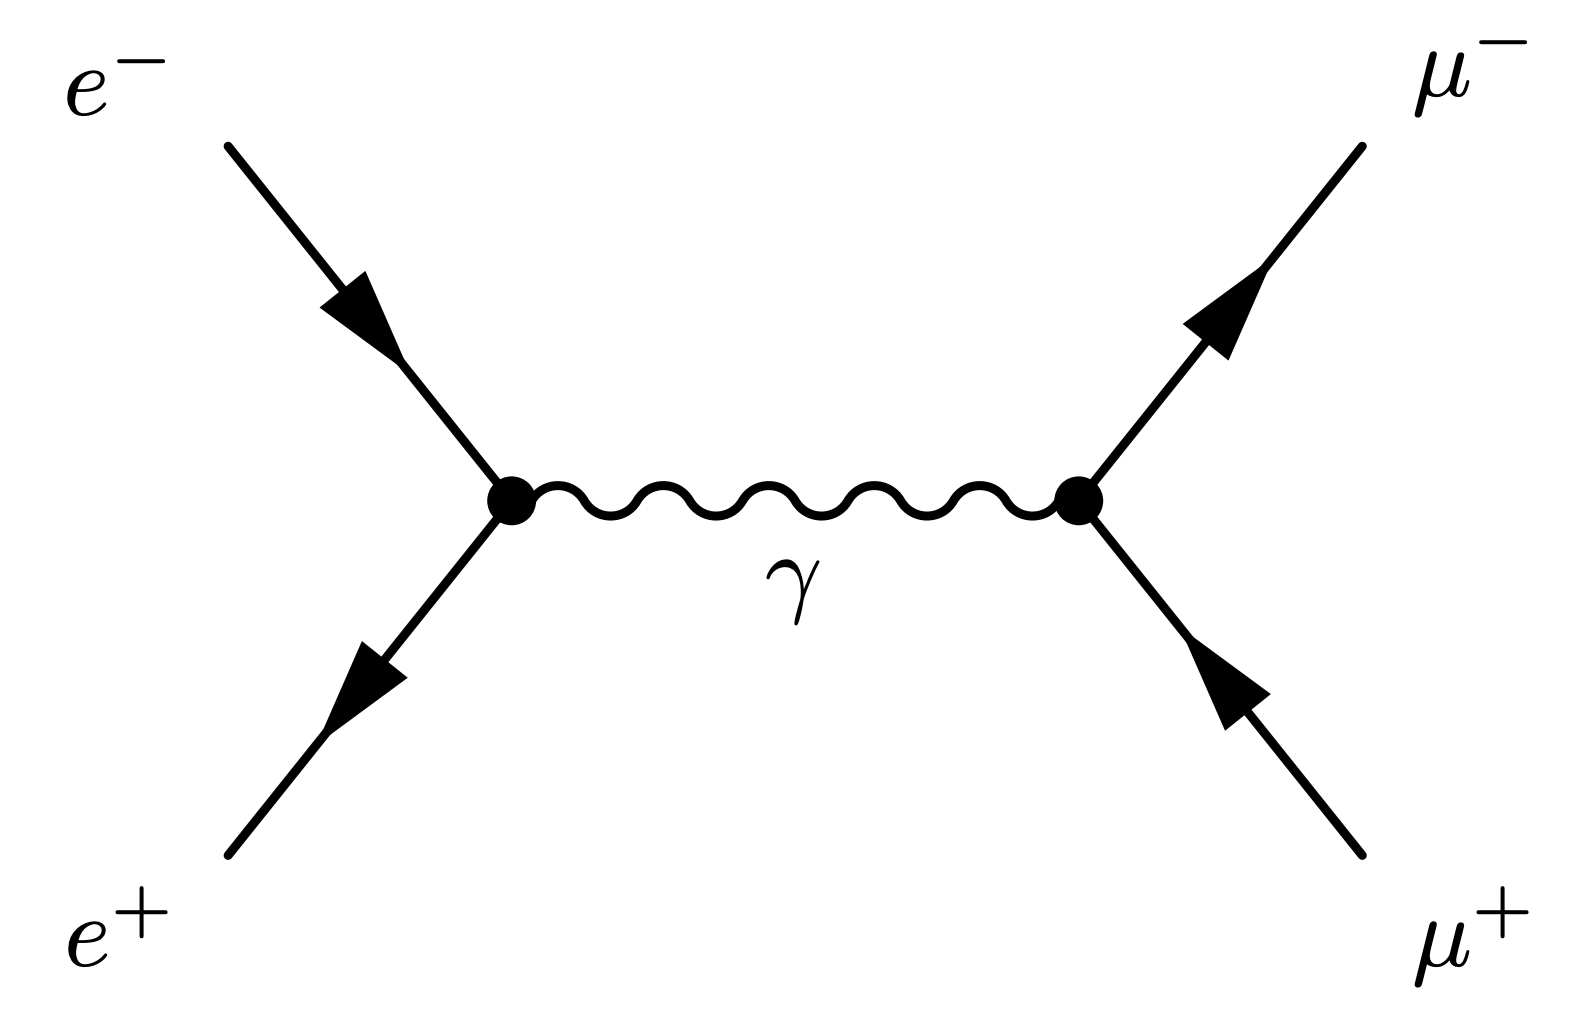
\includegraphics[width=0.5\linewidth]{plots/feynman_diagrams/feynman_e_to_mu.png}  \\
\caption[Electrons to Muons Feynman diagram]{Feynman diagram representing the tree-level process of $e^+ e^- \rightarrow \mu^+ \mu^-$. Electron and positron annihilate each other and produce muon-antimuon pair through a virtual photon.}
\label{fig:e-to-mu-feynman}
\end{figure}

\clearpage
\section{Symmetries}

In 1964, Richard Feynman gave a series of seven lectures called \emph{The Character of Physical Laws} at Cornell University, as part of the Messenger Lectures series. The lectures were videotaped by the BBC, and are available online alongside their transcripts~\cite{Feynman1997-vo}. It is such a precious piece of history, and I would recommend everyone to watch it, as it is meant for the public audience. It showcases not only Feynman's ability to explain complex ideas and theories, but also his funny and enchanting personality. The fourth lecture in that series is called \emph{Symmetry in Physical Laws}, in which he starts by describing how Weyl defines a symmetry:

\begin{quote}
So, Weyl said, a thing is symmetrical if there’s something that you can do to it, so that after you’re finished doing it, it looks the same as it did before. That is the sense in which we say that the laws of physics are symmetrical: that there are things that we can do to the physical laws, or to our way of representing the physical laws, which make no difference and leave everything unchanged in its effects.
\end{quote}

Most physicists will probably agree that's what they mean when they say that a physical law is symmetrical. In this chapter, we are concerned with symmetries of laws, rather than symmetries of objects, such as a human face, for example. In modern physics, largely thanks to Noether's theorem, symmetries became fundamental, and they set the foundations of the Standard Model of particle physics. In this chapter, I summarize the reasons why symmetries are so important and what roles they play in the Standard Model. But first, I would like to introduce my favorite physics riddle, which Feynman described, starting at minute 40:04 in the same lecture:

\begin{quote}
Suppose that we were in telephone conversation with a Martian or an Arcturian, or something. We don’t know where he is and we would like to describe things to him. We want to tell him about things. You say, so how’s he going to understand the words, well, that’s been studied very much by Professor Morrison here. He has pointed out that one way would be to start out and say tick tick two, tick tick tick three, and so on, and pretty soon the guy’d catch onto the numbers. Then—as he understands your number system, then—you can write lots of numbers and you could, for example, write a whole sequence of numbers that represents the weights, the proportional weights, of the different atoms, in succession.

Then say, hydrogen: 1.008, deuterium, and so on and so on. And he would-after he sat down with all those numbers and piddled around a while, would-discover that the mathematical ratios were the same as the ratios of the weights of the elements and, therefore, those names must be for the elements—and so gradually, you could, in talking to him, have a common language, in many ways, common. There are many-now comes the problem.

Suppose that he says, you fellas—after we get familiar with him, he says, "You’re very nice; now I’d like to know what you look like." And you start out, "Well, we’re about six feet tall." He says, "Six feet, how big is a foot?" "It’s very easy," you say; "six feet tall is 170 thousand million hydrogen atoms high." Well, it’s not a joke; it’s a possible way of describing six feet to someone that has no measure, assuming that we cannot send him any samples, nor can we both look at the same object.

If we have to tell him how big we are; we can do it. That’s because the laws of physics are not unchanged under a scale change. We can use that factor, use the properties of the scale to determine—I mean, you can use that fact to determine the scale.

Well, here we’ve described ourselves after telling six feet tall, and we’re so-and-so bilateral on the outside, and we look like this, and there are these prongs sticking out, and all this. And he says, "That’s very interesting; what do you look like on the inside?" So we describe the heart and so on, and we say, "Now, put the heart in on the left side."

Now the question is, how can we tell him which side is the left side?
\end{quote}

To put it shortly, the riddle is how to communicate the concept of left and right via radio signals to an alien civilization without reference to common sightings. Most physicists attempt to solve this problem by thinking of the right-hand rule in electromagnetism. Unfortunately, that would not work. The correct solution is very unexpected and one of the most surprising results of modern physics. The solution is explained in the section about discrete symmetries~\ref{sec:discrete-symmetries}.

\subsection{Conservation Laws}

A conservation law states that a particular measurable property of an isolated physical system does not change as the system evolves over time. Conservation laws are useful because they describe which processes can or cannot occur in nature. They also allow properties of the motion to be derived without solving the equations of motion. Conservation laws have changed throughout history, and some are a part of one theory but not another. Mass, for example, is conserved in classical mechanics, but not in relativity due to the principle of mass–energy equivalence. However, it is a good approximation when the assumptions of classical mechanics hold, such as low velocities and energies, and large enough objects. Most conservation laws are exact, or absolute, in the sense that they apply to all possible processes. Some conservation laws are partial, in that they hold for some processes but not for others.

In continuum mechanics, the most general form of an exact conservation law is given by a continuity equation. For example, conservation of electric charge $q$ is
\begin{equation}
\pdv{\rho}{t}=-\nabla\cdot\vb{j},
\end{equation}
where $\rho$ is the density of $q$ (amount per unit volume), $\vb{j}$ is the flux of $q$ (amount crossing a unit area in unit time), and $t$ is time. There are several methods for identifying conservation laws. It can be hypothesized and proved mathematically. In classical mechanics, Hamilton–Jacobi equations provide a method for identifying constants of motion, and so does Poisson's theorem. In QM, an observable quantity $Q$ will be a constant of motion if it commutes with the Hamiltonian, and it does not itself depend explicitly on time. In the context of particle physics, the most powerful theorem invoked in order to study conservation laws is Noether's theorem~\ref{sec:noethers-theorem}. It is also this theorem that connects conservation laws to symmetries, which is the topic of this section.

Currently, exact conservation laws that have never been proven to be violated include conservation of mass-energy $E$, conservation of linear momentum $\vb{p}$, conservation of angular momentum $\vb{L}$, conservation of electric charge, conservation of weak isospin, conservation of color charge, and conservation of CPT parity. Approximate conservation laws, \ie, conservation laws which are approximately true in particular situations, such as low speeds, short time scales, or certain interactions include conservation of mechanical energy, mass, flavor, strangeness, space-parity, charge-parity, time-parity, and CP parity.

\subsection{Noether's Theorem}
\label{sec:noethers-theorem}

In 1915, German-Jewish female mathematician Amalie Emmy Noether proved one of the most fundamental theorems of 20th-century modern physics. In the spring of that year, she was invited by David Hilbert and Felix Klein to join the Göttingen mathematics department, challenging the views of some of his colleagues that a woman should not be allowed to teach at a university. Soon after arriving at Göttingen, she demonstrated her capabilities by proving the theorem now known as Noether's theorem, which shows that a conservation law is associated with any differentiable symmetry of a physical system~\cite{Lederman2004-fl}. That made modern theoretical physicists much more focused on symmetries.

Informally, Noether's theorem can be stated as:
\begin{quote}
If a system has a continuous symmetry property, then there are corresponding quantities whose values are conserved in time.
\end{quote}
In the context of classical field theory, it can be stated as:
\begin{quote}
To each differentiable symmetry of a local Lagrangian, there corresponds a conserved current.
\end{quote}
Previously, we described a symmetry as something that you can do to a system, so that it looks the same as it did before. More formally in this context, a symmetry is the covariance of the form that a physical law takes, where by covariance, we mean the invariance of the form of physical laws under differentiable transformations. That means continuous transformations that leave the equations of motion invariant. Formally, in the context of classical field theories, the theorem can be stated in the language of fields~\cite{Peskin2019-bt}. Consider a continuous transformations on the fields $\phi$, which in infinitesimal form can be written
\begin{equation}
\phi(x)\rightarrow\phi^\prime(x)=\phi(x)+\alpha\Delta\phi(x),
\label{eq:infi-trans}
\end{equation}  
where $\alpha$ is an infinitesimal parameter and $\Delta\phi(x)$ is some deformation of the field configuration. It is considered a symmetry if it leaves the equations of motion invariant. This is ensured either if the action is invariant under the transformation or if it is changed by a surface term. The Lagrangian, therefore, must be invariant under  the transformation in Equation~\ref{eq:infi-trans} up to a 4-divergence:
\begin{equation}
\mathcal{L}(x)\rightarrow\mathcal{L}(x)+\alpha\partial_{\mu}\mathcal{J}^{\mu}(x),
\end{equation}
for some $\mathcal{J}^{\mu}$. After varying the fields, one finds:
\begin{equation}
\partial_{\mu}j^{\mu}=0,\qquad \textrm{for} \quad j^{\mu}(x)=\pdv{\mathcal{L}}{\qty(\partial_{\mu}\phi)}\Delta\phi-\mathcal{J}^{\mu}.
\end{equation}
This result states that the current $j^{\mu}(x)$ is conserved. This can also be expressed by saying that the charge
\begin{equation}
Q\equiv\int_{\textrm{all space}}j^0\dd[3]{x}
\end{equation}
is a constant in time.

\clearpage
\subsection{Groups}

We have seen that symmetries lead to conservation laws via Noether's theorem. Intuitively, we stated that symmetries are things that don't change while other things do change. The mathematical description of symmetries is Group Theory~\cite{Robinson2011-dv}. Groups are fundamental in particle physics, since they describe the symmetries which the laws of physics seem to obey. The first example encountered in particle physics is Lorentz covariance, or Lorentz symmetry. It is an equivalence of observation or observational symmetry due to special relativity, implying that the laws of physics stay the same for all observers that are moving with respect to one another within an inertial frame. Mathematically speaking, a physical quantity is said to be Lorentz covariant if it transforms under a given representation of the Lorentz group. In particular, a Lorentz covariant scalar (\ie, the space-time interval) remains the same under Lorentz transformations and is said to be a Lorentz invariant. Another important example is gauge theories. A gauge theory is a type of field theory in which the Lagrangian does not change (is invariant) under local transformations according to certain smooth families of operations (Lie groups).

A \emph{Group}, denoted $\qty(G, \star)$, is a set of object, denoted $G$, and some operation on those objects, denoted $\star$, subject to the following:
\begin{enumerate}
\item For any two elements $g_1$ and $g_2$ in $G$, the elemet $g_1\star g_2$ is also in $G$. This property is called \emph{closure}.
\item For any three elements $g_1, g_2$ and $g_3$ in $G$, the relation $\qty(g_1\star g_2)\star g_3=g_1\star\qty(g_2\star g_3)$ must hold. This property is called \emph{associativity}.
\item There exists an element of $G$ which we will denote $e$, that satisfies $e\star g = g\star e = g$ for every element $g$ of $G$. This property is called \emph{identity}.
\item For every element $g$ of $G$, there is another element of $G$ which we will denote $g^{-1}$ that satisfies $g^{-1}\star g = g\star g^{-1}=e$. This property is called \emph{inverse}.
\end{enumerate}
A group in which $g_i\star g_j=g_j\star g_i$ is called \emph{abelian}. Otherwise, it is non-abelian. Groups can be \emph{discrete} or \emph{continuous}. We will mainly concern ourselves with continuous groups. It is easy to see that Lorenz transformations and gauge transformation form continuous groups.

A \emph{representation} of a group $G$ on a vector space $V$ over a field $K$ is a group homomorphism from $G$ to $GL(V)$, the general linear group on $V$. That is, a representation is a map
\begin{equation}
\rho:G\rightarrow GL(V)
\end{equation}
such that
\begin{equation}
\rho\qty(g_1 g_2)=\rho\qty(g_1)\rho\qty(g_2),\qquad \textrm{for all}\,\, g_1,g_2\in G.
\end{equation}
In other words, a representation assigns a matrix to each element of the group, while the operation is represented by regular matrix multiplication and preserves the group multiplication table. A subspace $W$ of $V$ that is invariant under the group action is called a \emph{subrepresentation}. If $V$ has exactly two subrepresentations, namely the zero-dimensional subspace and $V$ itself, then the representation is said to be \emph{irreducible}; if it has a proper subrepresentation of nonzero dimension, the representation is said to be \emph{reducible}. 

\subsubsection{Lie Groups}

Symmetries in the SM are usually parameterized by continuous variables. This means that we are no longer talking about $g_i$'s but about $g(\theta)$. Groups that are parameterized by one or more continuous variables are called \emph{Lie Groups}. In continuously generated groups, there are elements close to the identity such that a general element can be reached by repeated action of these infinitesimal elements. Any infinitesimal group element $g$ can be written
\begin{equation}
g\qty(\alpha)=1+i\alpha^aT^a+\order{\alpha^2}.
\end{equation}
The set $T^a$ are Hermitian operators called the \emph{generators} of the symmetry group. They obey commutation relations
\begin{equation}
\comm{T^a}{T^b}=i f^{abc}T^c;
\end{equation}
the numbers $f^{abc}$ are called \emph{structure constants}. The vector space spanned by the generators, with the additional operation of commutation, is called a \emph{Lie Algebra}. The structure constants obey the Jacobi identity
\begin{equation}
f^{ade}f^{bcd}+f^{bde}f^{cad}+f^{cde}f^{abd}=0.
\end{equation}
If the structure constants are known, the entire group can be determined in any representation desired. A particular set of generators defines a particular representation of a group. Any element of a group in a particular representation can be written as
\begin{equation}
D(\alpha)=e^{i\alpha^{a}T^{a}}.
\end{equation}

\subsection{Gauge Theory}
\label{sec:gauge-theory}

As described before, a gauge theory is a type of field theory in which the Lagrangian is invariant under local transformations according to certain smooth families of operations, which form Lie groups. The groups formed by the gauge transformations are referred to as the symmetry groups or the gauge groups of the theory. For each group generator, there necessarily arises a corresponding field (usually a vector field) called the gauge field. When such a theory is quantized, the quanta of the gauge fields are called gauge bosons. If the symmetry group is non-commutative, then the gauge theory is referred to as a non-abelian gauge theory, with the usual example being the Yang–Mills theory. The SM is a non-abelian gauge theory with the symmetry group $U(1)\cross SU(2)\cross SU(3)$, which demonstrate the successful central role that gauge theory plays in theories explaining the dynamics of elementary particles.

\subsubsection{Demonstration: Electrodynamics}

The Lagrangian that generates the electron field's Dirac equation is
\begin{equation}
\mathcal{L}=\bar{\psi}\qty(i\gamma^{\mu}\partial_{\mu}-m)\psi.
\end{equation}
This Lagrangian has a \emph{global symmetry} of
\begin{equation}
\psi\mapsto e^{i\theta}\psi.
\end{equation}
It is global in that it acts on the field in the exact same way at every point in spacetime. The gauge group here is $U(1)$, also known as \emph{the circle group}, the multiplicative group of all complex numbers with absolute value 1, that is, the unit circle in the complex plane or simply the unit complex numbers.

Next we are \emph{gauging the symmetry}. This means that we are making the global symmetry local by making $\theta$ depend on spacetime
\begin{equation}
\theta=\theta(x),
\end{equation}
and then try to force the Lagrangian to maintain its invariance under the \emph{local} $U(1)$ transformation. Define a new field $A_{\mu}$, which transforms under the $U(1)$ transformation $e^{i\theta(x)}$ according to
\begin{equation}
A_\mu\mapsto A_\mu-\frac{1}{q}\partial_{\mu}\alpha(x).
\end{equation}
$A_{\mu}$ is called the \emph{Gauge Field}. It is introduced by replacing the standard derivative $\partial_{\mu}$ with the \emph{Covariant Derivative}
\begin{equation}
D_{\mu}=\partial_{\mu}+iqA_{\mu}.
\end{equation}
This results in the Lagrangian
\begin{equation}
\mathcal{L}=\bar{\psi}\qty(i\gamma^{\mu}D_{\mu}-m)\psi=\bar{\psi}\qty(i\gamma^{\mu}\partial_{\mu}-m-q\gamma^{\mu}A_{\mu})\psi=\bar{\psi}\qty(i\gamma^{\mu}\partial_{\mu}-m)\psi-qj^{\mu}A_{\mu},
\end{equation}
where $j^{\mu}=\bar{\psi}\gamma^{\mu}\psi$ is the $U(1)$ conserved current. This Lagrangian is invariant under the local $U(1)$ symmetry. Adding an appropriate gauge-invariant kinetic term 
\begin{equation}
\mathcal{L}_{\textrm{Kinetic}}=-\frac{1}{4}F_{\mu\nu}F^{\mu\nu}
\end{equation}
where
\begin{equation}
F^{\mu\nu}=\frac{i}{q}\comm{D^\mu}{D^\nu}
\end{equation}
and $q=e$ is the constant of proportionality , and $D^\mu$ is the covariant derivative. This results in the Lagrangian used as the starting point in quantum electrodynamics
\begin{equation}
\mathcal{L}=\bar{\psi}\qty(i\gamma^{\mu}D_{\mu}-m)\psi-\frac{1}{4}F_{\mu\nu}F^{\mu\nu}.
\end{equation}
The gauge symmetry $U(1)$ created therefore a theory with electromagnetism. The field $A_{\mu}$ will become the photon upon quantization.

\subsection{Symmetries of the Standard Model}
\label{symmetries-of-the-standard-model}

The symmetries of the SM arise from  global spacetime symmetries involving transformations of space and time, and from local gauge symmetries, explained in Section~\ref{sec:gauge-theory}. The fields in the theory then fall into representations of these groups.

\subsubsection{Poincaré Group}

The Poincaré group represents the full spacetime symmetry of special relativity. It is this group that makes the Standard Model a relativistic quantum theory. As a result, all elementary particles fall in representations of this group. The Poincaré group is a ten-dimensional noncompact Lie group, and a semi-direct product of the translations group and the Lorentz group. It includes:
\begin{itemize}
\item \emph{translations} (displacements) in time and space ($\vb{P}$), forming the abelian Lie group of translations on space-time;
\item \emph{rotations} in space, forming the non-abelian Lie group of three-dimensional rotations ($\vb{J}$);
\item \emph{boosts}, transformations connecting two uniformly moving bodies ($\vb{K}$).
\end{itemize}
The last two symmetries, $\vb{J}$ and $\vb{K}$, together make the Lorentz group. The group has 10 generators, which imply by Noether's theorem 10 conservation laws: 1 for the energy, 3 for the momentum, 3 for the angular momentum and 3 for the velocity of the center of mass.

The Lorentz group is the set of all Lorentz transformations. A \emph{Lorentz transformations} is a linear, homogeneous change of coordinates from $x^{\mu}$ to $\bar{x}^{\mu}$,
\begin{equation}
\bar{x}^{\mu}=\tensor{\Lambda}{^{\mu}_{\nu}}x^{\nu}
\end{equation}
that preserves the interval $x^2$ between $x^{\mu}$ and the origin, where
\begin{equation}
x^2\equiv x^{\mu} x_{\mu}=g_{\mu\nu}x^{\mu}x^{\nu}=\vb{x}^2-c^2t^2.
\end{equation}
This means that the matrix $\tensor{\Lambda}{^{\mu}_{\nu}}$ must obey
\begin{equation}
g_{\mu\nu}\tensor{\Lambda}{^{\mu}_{\rho}}\tensor{\Lambda}{^{\nu}_{\sigma}}=g_{\rho\sigma},
\end{equation}
where $g_{\mu\nu}$ is the Minkowski metric. The group algebra is defined by the commutation relations of its generators
\begin{equation}
\begin{split}
\comm{J_i}{J_j}&=i\epsilon_{ijk}J_k, \\
\comm{J_i}{K_j}&=i\epsilon_{ijk}K_k, \\
\comm{K_i}{K_j}&=-i\epsilon_{ijk}J_k, \\
\end{split}
\end{equation}
corresponding to the two types of transformation: rotations and boosts. Consider the following linear combinations of the generators:
\begin{equation}
N^{\pm}_{i}=\frac{1}{2}\qty(J_i\pm iK_i).
\end{equation}
The resulting commutation relations of these operators are
\begin{equation}
\begin{split}
\comm{N_i^+}{N_j^+}&=i\epsilon_{ijk}N_k^+, \\
\comm{N_i^-}{N_j^-}&=i\epsilon_{ijk}N_k^-, \\
\comm{N_i^-}{N_j^+}&=0. \\
\end{split}
\end{equation}
Therefore, we see that we have two copies of $SU(2)$. This is a very useful fact, since it shows that any representation of the Lorenz group $SO(1,3)$ can be specified by the doublet $(j,j')$, where $j$ corresponds to the $SU(2)$ generated by the $N_i^+$'s and $j'$ corresponds to the $SU(2)$ generated by the $N_i^-$'s. The corresponding representation of the Lorentz group will be made up of $(2j+1)(2j'+1)\times (2j+1)(2j'+1)$ matrices. The four simplest and most often encountered representations are:
\begin{equation}
\begin{split}
&(0,0)=\text{\emph{Scalar} or \emph{Singlet}}\\
&(\frac{1}{2},0)=\text{\emph{Left-handed spinor}}\\
&(0,\frac{1}{2})=\text{\emph{Right-handed spinor}}\\
&(\frac{1}{2},\frac{1}{2})=\text{\emph{Vector}}
\end{split}
\end{equation}

\subsubsection{Discrete Symmetries: P, T, C}
\label{sec:discrete-symmetries}

A theory can possess or be tested against discrete symmetries. In addition to continuous Lorentz transformations, there are two other spacetime operations that are potential symmetries of the Lagrangian: \emph{parity} and \emph{time reversal}. Parity, denoted by $P$, sends $(t,\vb{x})\rightarrow(t,-\vb{x})$, reversing the handedness of space. Time reversal, denoted $T$, sends $(t,\vb{x})\rightarrow(-t,\vb{x})$, interchanging the forward and backward light-cones. A third (non-spacetime) discrete operation is \emph{charge conjugation}, denoted by $C$. Under this operation, particles and antiparticles are interchanged.

Experimentally, it is known that the gravitational, electromagnetic, and strong interactions are symmetric with respect to $P$, $C$, and $T$. The weak interactions violate $C$ and $P$ separately but preserve $CP$ and $T$ approximately. But certain rare processes involving neutral $K$ mesons also show $CP$ and $T$ violation. All observations indicate that $CPT$ is a perfect symmetry of Nature.

That brings us to the riddle from the beginning of the chapter. How do we communicate the concept of left and right? The answer lies in parity symmetry. If a force is symmetric under parity, nature does not differentiate between our world and the mirror world. That means we cannot use gravity, electromagnetism, or the strong nuclear force to solve that riddle. The only force that breaks this symmetry is parity. In 1956, the Chinese-American female physicist Chien-Shiung Wu conducted the Wu experiment, which demonstrated that parity was violated by the weak interaction, providing a way to operationally define left and right without reference to the human body. The experiment monitored the decay of cobalt-60 atoms aligned by a uniform magnetic field. This beta decay can be written as:
\begin{equation}
\tensor*[^{60}_{27}]{\mathrm{Co}}{}\rightarrow\tensor*[^{60}_{28}]{\mathrm{Ni}}{}+\Pem+\PAGne+2\PGg.
\end{equation}
It has been observed that most of the electrons favored a very specific direction of decay, specifically opposite to that of the nuclear spin. It was later established that parity violation was, in fact, maximal. Since the direction of the spin of the cobalt atoms is known, the favored direction of the electrons will define the direction left. The only catch here is that we've assumed the aliens are made from matter, rather than antimatter. If they build a human being and that human being comes to visit us, we should be careful. Or, in the words of Feynman:
\begin{quote}
Then when we go finally to meet this man (after he tells us how to build a sufficiently good spaceship), we go to meet this man, and you walk up to him and you put out your right hand to shake hands—if he puts out his right hand, okay, but if he puts out his left hand, watch out, because the two of you will annihilate with each other!
\end{quote}

\subsubsection{Gauge Symmetries}

The local $SU(3)\times SU(2) \times U(1)$ gauge symmetry is an internal symmetry that essentially defines the SM. Roughly, the three factors of the gauge symmetry give rise to the three fundamental interactions. The fields fall into different representations of the various symmetry groups of the Standard Model. It has been explained in Section~\ref{sec:gauge-theory} how gauging a symmetry gives rise to interactions. The electroweak sector is a Yang–Mills gauge theory with the symmetry group $SU(2)_L \times U(1)_Y$, while quantum chromodynamics is a Yang–Mills gauge theory with $SU(3)$ symmetry. The massless gauge bosons of the electroweak $SU(2)_L \times U(1)_Y$ mix after spontaneous symmetry breaking to produce the 3 massive weak bosons ($\PWp$, $\PWm$, and $\PZ$) as well as the still-massless photon field. The dynamics of the photon field and its interactions with matter are, in turn, governed by the $U(1)$ gauge theory of quantum electrodynamics.

\subsubsection{Spontaneous Symmetry Breaking}
\label{spontaneous-symmetry-breaking}

Spontaneous symmetry breaking is a process by which a physical system in a symmetric state spontaneously ends up in an asymmetric state. It can describe systems where the equations of motion or the Lagrangian obey symmetries, but the lowest-energy vacuum solutions do not exhibit the same symmetry. In the SM, without spontaneous symmetry breaking, all particles would be massless due to the gauge symmetries. The Higgs mechanism provides a spontaneous symmetry breaking mechanism, which is essential to explain the generation mechanism of mass for gauge bosons as well as the fermions. It was developed by Higgs, Brout and Englert in the 1960s~\cite{Higgs:1964ia,Higgs:1964pj,Englert:1964et,Guralnik:1964eu,Higgs:1966ev}. Based on work from Sheldon~\cite{PhysRev.155.1554} it was later applied to $SU(2)_L \times U(1)_Y$ gauge theory by Weinberg and Salam~\cite{GLASHOW1961579,Weinberg:1967tq,Salam:1968rm}.

In order to achieve the breaking mechanism, the Higgs field is added to the Standard Model. The Higgs field is a scalar field, with two neutral and two electrically charged components that form a complex doublet of the weak isospin $SU(2)$ symmetry. It has a "Mexican hat-shaped" potential. This shape means that at low energies, the Higgs field in its ground state takes less energy to have a nonzero vacuum expectation value (VEV) than a zero value. This VEV breaks the weak isospin $SU(2)$ symmetry of the electroweak interaction. Then, three components of the Higgs field are "absorbed" by the $SU(2)_L \times U(1)_Y$ gauge bosons, to give $\PWp$, $\PWm$, and $\PZ$ bosons their mass, while the remaining electrically neutral component either manifests as a Higgs boson, or couples to the fermions via Yukawa couplings, causing them to acquire mass as well.

\clearpage
\section{The Standard Model}

The Standard Model (SM) of particle physics is the most successful theory we have for explaining the fundamental particles and their interactions (electromagnetic, weak, and strong interactions – excluding gravity). Thus far, no fundamental particle beyond the SM has been observed. Its formulation has been finalized in the mid-1970s and was driven by theoretical and experimental particle physicists alike. Important milestones in the development and experimental observations are spread over many decades. In 1954, Yang Chen-Ning and Robert Mills extended the concept of gauge theory from abelian groups to nonabelian groups to provide an explanation for strong interactions~\cite{PhysRev.96.191}, as we have seen in Section~\ref{sec:gauge-theory}. In 1957, the Wu experiment demonstrated that parity was not conserved in the weak interaction~\cite{PhysRev.105.1413}, as was described in~\ref{sec:discrete-symmetries}. In 1961, Glashow combined the electromagnetic and weak interactions~\cite{GLASHOW1961579}. In 1967, Weinberg~\cite{Weinberg:1967tq} and Salam~\cite{Salam:1968rm} incorporated the Higgs mechanism~\cite{Englert:1964et,Higgs:1964pj,Guralnik:1964eu} into Glashow's electroweak interaction, giving it its modern form. In 1973, the neutral weak currents caused by Z boson exchange were discovered at CERN~\cite{HASERT1973121,HASERT1973138,HASERT19741}. In 1983, the $\PWpm$ and $\PZz$ bosons were discovered experimentally~\cite{RevModPhys.71.S96}. The top quark was discovered in 1995 by the CDF~\cite{PhysRevLett.74.2626} and DØ~\cite{PhysRevLett.74.2632} experiments at Fermilab. The discovery of the tau neutrino was announced in July 2000 by the DONUT collaboration~\cite{Kodama_2001}. In 2012, both CMS~\cite{201230} and ATLAS~\cite{20121} at CERN have announced that they observed the Higgs boson, the final fundamental particle predicted by the SM to be experimentally confirmed.

Formally, the mathematical framework of the SM is a relativistic quantum field theory, in which a Lagrangian controls the dynamics and kinematics, as was introduced in Section~\ref{sec:rqft}. The construction of the SM is done by postulating a set of symmetries of the system, and then by writing down the most general renormalizable Lagrangian from its particle (field) content that obeys these symmetries. As a relativistic quantum field theory, the global Poincaré symmetry is postulated. The local $SU(3)\times SU(2) \times U(1)$ symmetry is an internal symmetry that essentially defines the SM. The symmetries and how gauge invariance gives rise to the gauge bosons were described in Sections~\ref{sec:gauge-theory} and~\ref{symmetries-of-the-standard-model}. The strong force is described by the group $SU(3)$, which acts on the color charge $C$. The electroweak force is described by the group $SU(2) \times U(1)$ and acts on the weak hypercharge $Y$ and on left-handed fermions, which have a weak isospin $T_3\neq 0$.

The SM predicts fundamental particles, which are shown in Figure~\ref{fig:sm-particles}. They can be categorized in different ways according to their quantum numbers. The matter particles are \emph{fermions}, which have half-integer spin, specifically spin $1/2$. They interact with each other through the exchange of gauge bosons, which have spin 1. Only particles that carry the charge associated with an interaction can interact with the gauge bosons. In addition, the SM predicts the Higgs boson, which has spin 0, and is a result of the Higgs field. The Higgs field is responsible for the spontaneous symmetry breaking described in Section~\ref{spontaneous-symmetry-breaking} and generates the masses of the massive particles in the SM.

\begin{figure}[!htb]
\centering
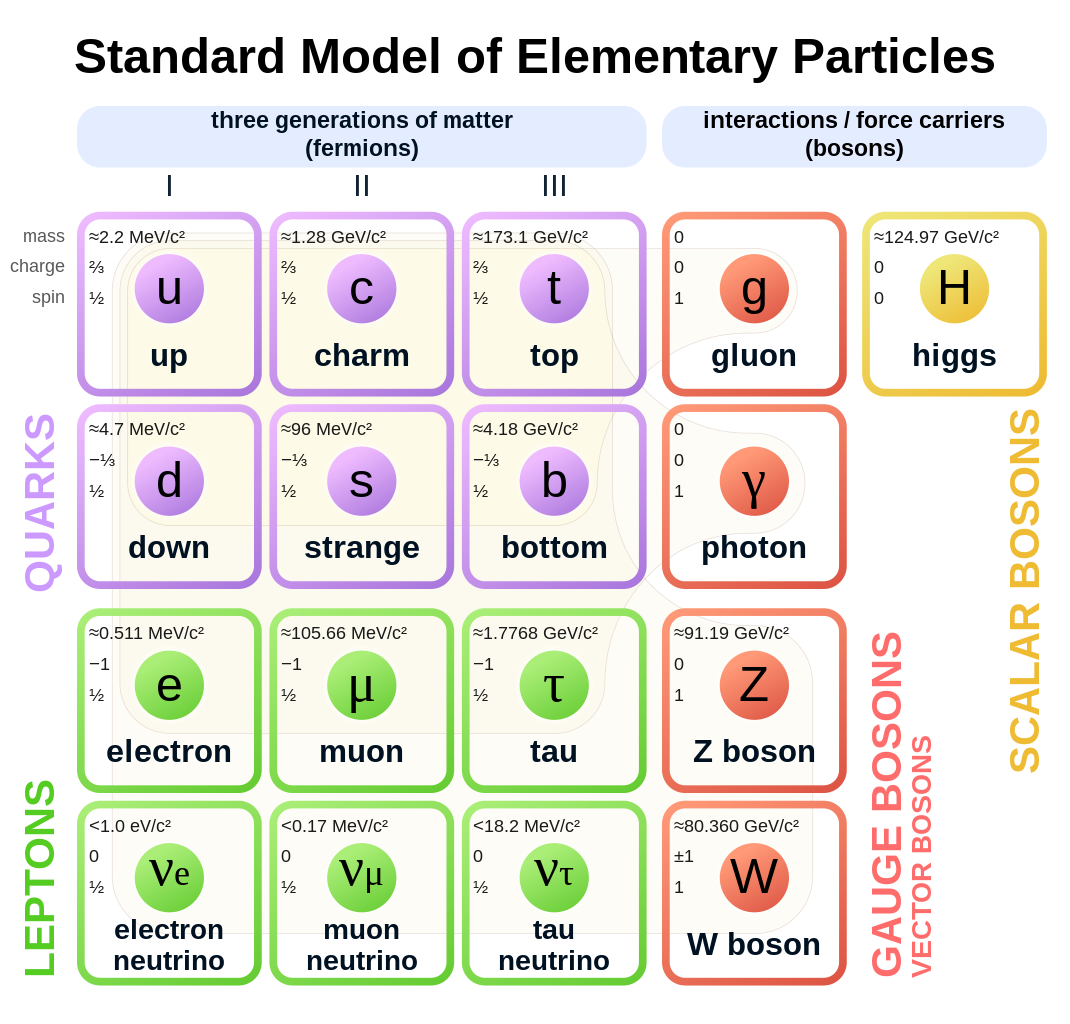
\includegraphics[width=0.5\linewidth]{plots/sm/Standard_Model_of_Elementary_Particles.svg.png}  \\
\caption[Elementary particles of the Standard Model]{Elementary particles of the Standard Model, including the most important quantum numbers.}
\label{fig:sm-particles}
\end{figure}

\subsection{Fermions}

According to the spin-statistics theorem, fermions respect the Pauli exclusion principle. Each fermion has a corresponding antiparticle. They can be classified further according to how they interact, or equivalently, by the charges they carry. There are six flavored quarks: up ($\PQu$), down ($\PQd$), charm ($\PQc$), strange ($\PQs$), top ($\PQt$), bottom ($\PQb$), and each has a corresponding antiparticle. They are divided into three generations, with each generation being heavier than the previous one. They are further grouped into up-type quarks ($\PQu$, $\PQc$, $\PQt$) and down-type quarks ($\PQd$, $\PQs$, $\PQb$). Quarks carry color charge, and hence interact via the strong interaction. The quarks are strongly bound to one another due to the phenomenon of color confinement. Therefore, they form color-neutral composite particles called hadrons, which can contain either a quark and an antiquark (mesons) or three quarks (baryons). Quarks also carry electric charge and weak isospin, allowing them to participate in electromagnetic and weak interactions.

In contrast to quarks, leptons do not carry a color charge and, therefore, do not participate in strong interactions. There are six flavored leptons: the electron (\Pe), the electron neutrino (\PGne), the muon (\PGm), the muon neutrino (\PGnGm), the tau (\PGt), and the tau neutrino (\PGnGt). Each lepton has a corresponding antiparticle. Leptons are also divided into three generations based on their masses. Since each member of a generation has a greater mass than the corresponding particle of any previous generation, the charged particles of the first generation do not decay. That's why all ordinary (baryonic) matter is made up of particles from the first generation.

The SM is a chiral theory, meaning that left-handed and right-handed fermions are treated differently. Under weak isospin $SU(2)$ transformations, the left-handed particles are weak-isospin doublets, whereas the right-handed particles are singlets. That means that all left-handed fermions have a weak isospin of $\pm 1/2$,  while the right-handed fermions have a weak isospin of 0. The charged left-handed leptons and the left-handed neutrinos of each generation are arranged as weak isospin doublets. The right-handed charged leptons are singlets. Right-handed neutrinos are not included in the original formulation of the SM. The weak hypercharge of the left-handed leptons is -1, while the right-handed leptons have a weak hypercharge of -2.

\subsection{Gauge bosons}

In the SM, gauge bosons are the force carriers that mediate the strong, weak, and electromagnetic fundamental interactions. The gauge bosons all have a spin of 1. Photons mediate the electromagnetic force between electrically charged particles. The photon is massless and is described well by the theory of quantum electrodynamics. The $\PWp$, $\PWm$, and $\PZz$ gauge bosons mediate the weak interactions, and are massive. The weak interactions involving the $\PWpm$ act only on left-handed particles and right-handed antiparticles. The electrically neutral $\PZz$ boson interacts with both left-handed particles and right-handed antiparticles. Since the $\PWpm$ bosons carry electric charges of $+1$ and $-1$, they also couple to the photon. The eight gluons mediate the strong interactions between color-charged particles (the quarks). Gluons are massless, and because they carry color charge themselves, they can interact with each other. The strong interaction is governed by the theory of Quantum Chromodynamics (QCD). The interactions of the SM are summarized in Figure~\ref{fig:sm-interactions}.

\begin{figure}[!htb]
\centering
\includegraphics[width=0.5\linewidth]{plots/sm/Standard_Model_–_All_Feynman_diagram_vertices.svg.png}  \\
\caption[Interactions of the Standard Model.]{Interactions of the Standard Model~\cite{Lindon:2746537}. Feynman diagrams in the SM are built from combinations of these vertices. $q$ is any quark, $g$ is a gluon, $X$ is any charged particle, $\gamma$ is a photon, $f$ is any fermion, $m$ is any particle with mass, $m_B$ is any boson with mass.}
\label{fig:sm-interactions}
\end{figure}

The combined symmetry group $SU(2)_L \times U(1)_Y$ gives rise to four gauge bosons. The symmetry group $U(1)_Y$ gives rise to $B$, and $SU(2)_L$ gives rise to $W^1$, $W^2$, and $W^3$. The physical bosons $\gamma$, $\PWp$, $\PWm$, and $\PZz$ are obtained by mixing these states due to the Higgs mechanism and are given by
\begin{equation}
\PWpm=\frac{1}{\sqrt(2)}\qty(W^1\mp i W^2)
\end{equation}
and
\begin{equation}
\mqty(\PGg \\ \PZ)=\mqty(\cos \theta_W & \sin \theta_W \\ -\sin \theta_W & \cos \theta_W)\cdot \mqty(B \\ W^3),
\end{equation}
where $\theta_W$ is the mixing angle, or Weinberg angle. The electric charge is determined by the weak isospin and
weak hypercharge by
\begin{equation}
Q=T_3+\frac{Y}{2}.
\end{equation}

Generally speaking, the weak interaction is responsible for processes such as radioactive decay. It has the ability to change flavors. In a neutron decay, for example, a down quark in the neutron emits a $\PWm$ boson, thereby changing into an up quark. The $\PWm$ boson then decays into an electron and an electron antineutrino. This process is not restricted to quarks within one generation. The probability of a transition from one flavour j quark to another flavour i quark is encoded in the Cabibbo–Kobayashi–Maskawa (CKM) matrix and is proportional to $\abs{V_{ij}}^2$. The three diagonal elements of the matrix are close to unity, which means decay processes within the same generation are favored, whereas the off-diagonal elements are small, especially for mixing with the third generation. The weak force also causes neutrino oscillations due to mismatch of quantum states of neutrinos when they propagate freely and when they take part in weak interactions. The Pontecorvo–Maki–Nakagawa–Sakata matrix (PMNS matrix) encodes the amplitude of the transitions between mass eigenstates and flavor eigenstates.

The strong interaction is referred to as Quantum Chromodynamics (QCD). QCD describes interactions between quarks mediated by gluons. It is a non-abelian gauge theory, with symmetry group $SU(3)$. The QCD analogue of electric charge is a property called color. Gluons are the force carriers of the theory, just as photons are for the electromagnetic force in quantum electrodynamics. The three kinds of charge in QCD are referred to as \emph{color charge}: red, green, blue, and their anticolors. The strong interaction is responsible for the nuclear force, which binds protons and neutrons in the nucleus. It also binds quarks together to form hadrons, including nucleons.

\subsection{Higgs Boson}

As mentioned in Section~\ref{spontaneous-symmetry-breaking}, the Higgs mechanism is responsible for the spontaneous symmetry breaking of the $SU(2)_L \times U(1)_Y$ gauge group, which generates mass for all the massive particles in the SM. The Higgs boson is a consequence of the Higgs field. The mass term arising from the Dirac Lagrangian (for any fermion $\psi$) is $-m\bar{\psi}\psi$, which is not invariant under the chiral electroweak symmetry. In addition, the W and Z bosons are massive, which is unlike what is predicted without symmetry breaking. To solve these problems, the Higgs mechanism is introduced. In the Standard Model, the Higgs field is a complex scalar field that forms an $SU(2)_L$ doublet:
\begin{equation}
\phi=\frac{1}{\sqrt{2}}\mqty(\phi^+ \\ \phi^0),
\end{equation}
where the superscripts + and 0 indicate the electric charge (Q) of the components. The weak hypercharge of both components is 1. The Higgs potential is symmetric with respect to the origin and has a non-trivial minimum. It is given by
\begin{equation}
V(\phi)=\mu^2\abs{\phi}^2+\lambda\abs{\phi}^4,
\end{equation}
where $\lambda>0,\mu^2<0$. In a unitarity gauge one can set $\phi^+=0$ and make $\phi^0$ real. Then $<\phi^0>=v$ is the non-vanishing vacuum expectation value of the Higgs field, which spontaneously breaks the symmetry of the electroweak model. It generates the Higgs boson $H$ with the mass
\begin{equation}
m_H=\sqrt{-2\mu^2}.
\end{equation}
The masses of the $\PW$ and $\PZ$ bosons are given by:
\begin{equation}
\begin{split}
m_\PW&=\frac{1}{2}gv \\
m_\PZ&=\frac{m_\PW}{\cos \theta_W}. \\
\end{split}
\end{equation}
Self-interaction terms of the Higgs boson are described by the coupling strength $\lambda$. The masses of the fermions are generated via the Yukawa couplings.

\subsection{Shortcomings of the Standard Model}

Although the SM is a very successful theory, it falls short of explaining all observations and open questions. It is, therefore, not regarded a \emph{theory of everything}, and it is agreed to be incomplete. Direct experimental evidence not explained in the SM include:
\begin{itemize}
\item \textbf{Gravity:} The SM does not account for gravity. That is perhaps one of the biggest challenges that physicists of our time face.
\item \textbf{Neutrino masses:} The phenomenon of neutrino oscillation suggest that the neutrinos have mass~\cite{Gonzalez_Garcia_2008}, in direct contradiction to the initial formulation of the SM which assumed that they have zero mass.
\item \textbf{Baryon asymmetry:} The SM does not explain the observed imbalance in baryonic matter and antibaryonic matter in the observable universe~\cite{Canetti_2012}. The CP violation accounted for in the SM is too small to explain why our universe is made mainly from matter and not almost equal amounts of matter and antimatter.
\item \textbf{Dark matter and dark energy:} The existence of dark matter is also not explained by the SM~\cite{Garrett_2011}. If it unclear yet if it is a particle, or a different kind of phenomenon, but if it is a particle, then the SM needs to be extended. The SM also does not account for the  universe's accelerating expansion as possibly described by dark energy.
\end{itemize}

In addition, the SM is seen by some to possess some conceptual deficiencies, such as:
\begin{itemize}
\item \textbf{Hierarchy problem:} The Higgs mechanism gives rise to the hierarchy problem if some new physics is present at high energy scales. If that is the case, severe fine tuning of the parameters is required between the bare mass of the Higgs boson, and the enormous loop corrections to the Higgs mass~\cite{Jegerlehner_2014}. A further discussion about this problem is given in Section~\ref{sec:naturalness}.
\item \textbf{Ad-hoc-ness:} The SM requires 26 numerical constants whose values are unrelated and arbitrary. It is also unclear why there are three generations of quark and leptons.
\item \textbf{Unification of forces:} the successful unification of the weak and electromagnetic forces suggest that a further unification with the strong force might be possible. This is referred to as a Grand-Unified-Theory (GUT) theory. In a GUT theory, the coupling strength of the interactions are expected to have the same magnitude at some high energy scale, which is not observed in the SM.
\end{itemize}

\clearpage
\section{Supersymmetry}

\glsreset{susy}\gls{susy} is a set of theories in which a symmetry that relates fermions and bosons is postulated~\cite{Peskin2019-bt,Garrett_2011,MARTIN_1998}. That is, a supersymmetry transformation turns a bosonic state into a fermionic state, and vice versa. The interest in \gls{susy} can be traced back to 1967, in which Coleman and Mandula proved a no-go theorem stating that spacetime and internal symmetries can only combine in a trivial way~\cite{PhysRev.159.1251}. This means that the charges associated with internal symmetries must always transform as Lorentz scalars. Also, there can be no change of the spin of particles. Fermions cannot change into bosons or vice versa. This was evaded in the 70s by different groups of physicists~\cite{GERVAIS1971632,HAAG1975257} with the discovery of \gls{susy}. It is done by loosening the restriction on the types of symmetries of a QFT, and in addition to Lie Algebras one can consider graded Lie Algebras whose operators anticommute. The first realistic supersymmetric version of the SM was proposed by Fayet and is known as the \gls{mssm}.

An operator $Q$ that generates transformations between bosonic and fermionic states must be an anti-commuting spinor, with
\begin{equation}
\begin{split}
Q\ket{\text{Boson}}=\ket{\text{Fermion}},\\
Q\ket{\text{Fermion}}=\ket{\text{Boson}}.
\end{split}
\end{equation}
Since $Q$ is a complex spinor, $Q^\dagger$ is also a symmetry generator. These operators carry spin angular momentum $1/2$, so that \gls{susy} is a spacetime symmetry. It has been demonstrated that the most general possibility of such operators is a collection of spin-$1/2$ operators with the anticommutation reations
\begin{equation}
\pb{Q^i_\alpha}{Q^{j\dagger}_\beta}=2\delta^{ij}\sigma^\mu_{\alpha\beta}P^\mu,
\end{equation}
with $i,j=1,\ldots,N$. All other anticommutation relations between the $Q$s and commutation relations between the $Q$s and $P$s vanish. In the following, the simplest case $N=1$ is considered. It is the simplest supersymmetric extension of the Poincaré algebra, or the Super-Poincaré algebra. The index $\alpha=1,2$ is the left-handed spinor components of the operator, and $P^\mu$ is the total energy-momentum. 

The single-particle states of a supersymmetric theory fall into irreducible representations of the supersymmetry algebra, called supermultiplets. Each supermultiplet contains both fermion and boson states, which are known as \emph{superpartners} of each other. The resulting commutation relation
\begin{equation}
\comm{Q}{P^2}=\comm{Q^{\dagger}_{\dot{\alpha}}}{P^2}=0
\end{equation}
implies that particles that are transformed into each other have the same eigenvalues of $P^2$, and therefore equal masses. The generators also commute with the generators of gauge transformations. That means that particles and their \emph{superpartners} must also share the same gauge charges.

Since we do not observe a bosonic superpartner to the electron, named \emph{selectron}, with the same mass as the electron, it is clear that supersymmetry must be a spontaneously broken symmetry. The specific mechanism of SUSY breaking is unknown, but usually, further terms that break SUSY explicitly are added by hand to the Lagrangian. However, since naturalness is often described as a motivation for introducing SUSY, it is required that the SUSY breaking terms still provide a solution to the hierarchy problem. This means that the effective Lagrangian contains only "soft" SUSY breaking, meaning that they violate SUSY but contain only mass terms and coupling parameters with a positive mass dimension.

\subsection{The Minimal Supersymmetric Standard Model}
\label{sec:MSSM}

The \glsreset{mssm}\gls{mssm} is an extension to the SM that realizes SUSY~\cite{MARTIN_1998}. It is minimal in regards to the number of new particle states and new interactions. In this extension, each of the known fundamental particles is in either a chiral or gauge supermultiplet, and must have a superpartner with spin differing by $1/2$ unit. The names for the spin-0 partners of the quarks and leptons are constructed by prepending an “s”, for scalar. They can therefore be called \emph{squarks} and \emph{sleptons}, or generally \emph{sfermions}. Their symbols normally contain a tilde ($\widetilde{\,\,\,}$). The MSSM contains two Higgs supermultiplets in order to prevent an electroweak gauge anomaly. The generic nomenclature for a spin-$1/2$ superpartner is to append “-ino” to the name of the SM particle, so the fermionic partners of the Higgs scalars are called \emph{higgsinos}. The vector bosons of the SM clearly reside in gauge supermultiplets. Their fermionic superpartners are generically referred to as \emph{gauginos}. The spin-$1/2$ superpartners of the electroweak gauge bosons are called \emph{winos} and \emph{binos}. Table~\ref{tab:chiral-supermultiplets} lists the chiral supermultiplets of the MSSM, while Table~\ref{tab:gauge-supermultiplets} lists the gauge supermultiplets of the MSSM.

\begin{table}[!htp]
	\centering
	\label{tab:chiral-supermultiplets}
		\caption{Chiral supermultiplets of the MSSM. The spin-0 fields are complex scalars, and the spin-$1/2$ fields are left-handed two-component Weyl fermions.
}
		%\vspace{1mm}
			\begin{tabular}{|l|c|c|c|}
\hline
Names                  & spin 0  & spin $1/2$ & $SU(3)_C,SU(2)_L,U(1)_Y$ \\ \hline\hline
\multirow{3}{*}{squarks, quarks} & $\qty(\widetilde{u}_L\,\widetilde{d}_L)$ & $\qty(u_L\,d_L)$ & $\qty(\mathbf{3},\mathbf{2},\frac{1}{6})$ \\  
                  & $\widetilde{u}^{*}_R$ & $u^{\dagger}_R$ & $\qty(\bar{\mathbf{3}},\mathbf{1},-\frac{2}{3})$ \\  
                  & $\widetilde{d}^{*}_R$ & $d^{\dagger}_R$  & $\qty(\bar{\mathbf{3}},\mathbf{1},\frac{1}{3})$ \\ \hline
\multirow{2}{*}{sleptons, leptons} & $\qty(\widetilde{\nu}\,\widetilde{e}_L)$ & $\qty(\nu\,e_L)$ & $\qty(\mathbf{1},\mathbf{2},-\frac{1}{2})$  \\ 
                  & $\widetilde{e}^{*}_R$ & $e^{\dagger}_R$ & $\qty(\mathbf{1},\mathbf{1},1)$ \\ \hline
\multirow{2}{*}{Higgs, higginos} & $\qty(H^{+}_u\,H^{0}_u)$ & $\qty(\widetilde{H}^{+}_u\,\widetilde{H}^{0}_u)$ & $\qty(\mathbf{1},\mathbf{2},+\frac{1}{2})$ \\ 
                  & $\qty(H^{0}_d\,H^{-}_d)$ & $\qty(\widetilde{H}^{0}_d\,\widetilde{H}^{-}_d)$ & $\qty(\mathbf{1},\mathbf{2},-\frac{1}{2})$ \\ \hline
\end{tabular}
\end{table}

\begin{table}[!htp]
	\centering
	\label{tab:gauge-supermultiplets}
		\caption{Gauge supermultiplets of the MSSM.
}
		%\vspace{1mm}
			\begin{tabular}{|l|c|c|c|}
\hline
Names                  & spin $1/2$  & spin 1 & $SU(3)_C,SU(2)_L,U(1)_Y$ \\ \hline \hline 
gluino, gluon & $\PSg$ & $\Pg$ & $\qty(\mathbf{8},\mathbf{1},0)$ \\  
                   \hline
winos, $\PW$ bosons & $\PSWpm\,\PSW^0$ & $\PWpm\,\PW^0$ & $\qty(\mathbf{1},\mathbf{3},0)$  \\  \hline
bino, $B$ boson & $\widetilde{B}^0$ & $B^0$ & $\qty(\mathbf{1},\mathbf{1},0)$ \\ 
                   \hline
\end{tabular}
\end{table}

The superpartners listed in Tables~\ref{tab:chiral-supermultiplets} and~\ref{tab:gauge-supermultiplets} are not necessarily the mass eigenstates of the theory. Electroweak symmetry breaking and SUSY breaking can cause mixing between the electroweak gauginos and the higgsinos, and within the various sets of squarks and sleptons and Higgs scalars that have the same electric charge. The gluino cannot mix since it is a color octet fermion and therefore does not have the appropriate quantum numbers to mix with any other particle. The neutral higgsinos, $\widetilde{H}^{0}_u$ and $\widetilde{H}^{0}_d$, and the neutral gauginos, $\widetilde{B}^0$ and $\PSW^0$, mix into four mass eigenstates called \emph{neutralinos}. The charged higgsinos, $\widetilde{H}^{+}_u$ and $\widetilde{H}^{-}_d$, and winos, $\widetilde{W}^+$ and $\widetilde{W}^-$, mix to form two mass eigenstates with charge $\pm 1$ called \emph{charginos}. The neutralinos are labeled $\PSGczDo,\PSGczDt,\PSGczDT,\PSGczDf$ in increasing order of mass, and the charginos are labeled $\PSGcpmDo,\PSGcpmDt$, also in increasing order of mass. In the gauge-eigenstate basis $\qty(\widetilde{B},\PSW^0,\widetilde{H}^{0}_d,\widetilde{H}^{0}_u)$, the neutralino mass matrix is given by:
\begin{equation}
M_N=\mqty(M_1 & 0 & -c_\beta s_W m_Z & s_\beta s_W m_Z\\
0 & M_2 &  c_\beta c_W m_Z & -s_\beta c_W m_Z \\
-c_\beta s_W m_Z & c_\beta c_W m_Z & 0 & -\mu\\
s_\beta s_W m_Z & -s_\beta c_W m_Z & -\mu & 0),
\end{equation}
where masses $M_1$ and $M_2$ are the $U(1)$ and $SU(2)$ gaugino masses, $\mu$ is the higgsino mass parameter, and $\tan \beta=v_u/v_d$ is the ratio of the vacuum
expectation values of the two neutral Higgs fields which break the electroweak symmetry. Here, $s_\beta=\sin\beta$, $c_\beta=\cos\beta$ and $s_W,c_W$ are the sine and cosine of the electroweak mixing
angle $\theta_W$. The mixing of the charged gauginos and charged higgsinos is given by the matrix:
\begin{equation}
M_C=\mqty(M_2 & \frac{1}{\sqrt{2}}gv_u\\
\frac{1}{\sqrt{2}}gv_d & \mu),
\end{equation}
where $g$ is the $SU(2)$ gauge coupling.

A neutralino state can approximate a particular gaugino or higgsino state. If $\abs{M_1}$ and $\abs{M_2}$ are small compared to $m_Z$ and $\abs{\mu}$, then $\PSGczDo$ would be nearly a pure photino. If $\abs{M_1}$ and $m_Z$ are small compared to $\abs{M_2}$ and $\abs{\mu}$, then $\PSGczDo$ would be nearly a pure bino. If $\abs{M_2}$ and $m_Z$ are small compared to $\abs{M_1}$ and $\abs{\mu}$ then the lightest chargino pair and neutralino would constitute a triplet of roughly
mass-degenerate pure winos. Finally, if $\abs{\mu}$ and $m_Z$ are small compared to $\abs{M_1}$ and $\abs{M_2}$, then the lightest chargino pair and neutralino would be nearly pure higgsino states. These cases lead to strikingly different phenomenology.

For reasons such as proton stability, suppression of neutrino masses, and the accidental globel $B-L$ symmetry of the SM that is not automatically conserved in a generic supersymmetric extension of the SM, an addition symmetry called R-parity is added to the MSSM. It is defined as
\begin{equation}
R=\qty(-1)^{3(B-L)+2S},
\end{equation}
where B is baryon number, L is lepton number, and S is the spin. This implies that all the particles of the SM have even R-parity, whereas their corresponding superpartners have odd R-parity. Moreover,
R-parity invariance also implies that the lightest supersymmetric particle (LSP) is absolutely stable. Usually, the lightest neutralino is assumed to be the LSP, and it makes an attractive candidate for dark matter. It is often called a \gls{wimp}.

There are three principal motivations for the MSSM. We have encountered the first one, and that is that the LSP is a good dark matter candidate~\cite{Garrett_2011}. The second motivation is that if the superpartners are near the TeV scale, then measured gauge couplings of the three gauge groups unify at high energies~\cite{PhysRevD.24.1681}. The third motivation for the MSSM, and also why it was originally proposed, is that it could solve the hierarchy problem~\cite{DIMOPOULOS1981150}. This problem is described further in Section~\ref{sec:naturalness}.

Since the MSSM has more than 100 parameters in addition to the SM, it makes phenomenological analysis quite impractical. Therefore, reasonable constraints can be imposed on the MSSM in order to reduce the number of free parameters. Such a selection of assumptions is done in a submodel of the MSSM called the phenomenological MSSM (pMSSM)~\cite{djouadi1999minimal,Berger_2009}. The following assumptions define the pMSSM:
\begin{itemize}
\item no new source of CP-violation;
\item no flavour changing neutral currents;
\item first and second generation universality.
\end{itemize}
These assumption reduce the number of SUSY parameters to 19.


\subsection{Naturalness}
\label{sec:naturalness}

One of the motivations for SUSY, and for the MSSM in particular, is that it is able to solve the hierarchy problem of the Higgs boson's mass. This problem is closely related to fine-tuning and naturalness. The physical principle of \emph{naturalness} was articulated by ’t Hooft and states that a small parameter is natural only when a symmetry is gained as it is set to zero~\cite{tHooft:1980xss,Seiberg_1993}. That means that in QFT, if a bare parameter is unnaturally set to zero, radiative corrections lead to a renormalized non-zero value. If a small renormalized value is desired without a symmetry, the bare value has to be fine-tuned.

Mathematically speaking, the problem is related to quantum corrections that the mass of the Higgs boson (squared) receives from the virtual effects of every particle that couples, directly or indirectly, to the Higgs field. For a Dirac fermion $f$ that couples to the Higgs field via a term in the Lagrangian $-\lambda_f H \bar{f}f$, the mass squared of the Higgs boson receives a correction of
\begin{equation}
\Delta m^2_H = -\frac{\abs{\lambda_f}^2}{8\pi^2}\Lambda^2_{\mathrm{UV}}+\ldots,
\end{equation} 
where $\lambda_f$ is the Yukawa coupling and $\Lambda^2_{\mathrm{UV}}$ is an ultraviolet momentum cutoff used to regulate the loop integral. Each of the leptons and quarks of the SM contributes such a correction, with the top quark being the largest contribution with $\lambda_f\approx 0.94$~\cite{MARTIN_1998}. If the cutoff is of the order of $M_P$, then the quantum correction is 30 orders of magnitude larger than the required value $m^2_H\approx-\qty(92.9\GeV)^2$ without radiative corrections. This, for some physicists, makes it difficult to understand why $m^2_H$ is so small. In other words, it seems unlikely that such large contributions will add up to a small number, and it is an example of fine-tuning.

If SUSY is present, these large contributions can be avoided by cancellations between fermionic loops and loops from complex scalar particles. For a scalar particle $S$ with mass $m_S$ and a Lagrangian term $-\Lambda_S\abs{H}^2\abs{S}^2$, the correction is given by
\begin{equation}
\Delta m^2_H = \frac{\lambda_S}{16\pi^2}\left[\Lambda^2_{\mathrm{UV}} -2m_S^2\ln(\Lambda_{\mathrm{UV}}/m_S) \ldots\right].
\end{equation}
Since in the MSSM, each of the quarks and leptons of the SM is accompanied by two complex scalars with $\lambda_S=\abs{\lambda_f}^2$, the $\Lambda^2_{\mathrm{UV}}$ contributions neatly cancel. While this cancellation is true for unbroken SUSY, broken SUSY scenarios will require some amount of fine-tuning. The amount of fine-tuning in the MSSM can be quantified~\cite{Feng_2013,PhysRevD.58.096004}. If one requires a reasonable amount of fine-tuning, that puts constraints on the phenomenology of the MSSM. A 10\% level of fine-tuning will require the existence of one pair of charginos and two neutralinos with a maximum mass of $200-300\GeV$~\cite{natural-SUSY,BARBIERI198863,Antusch_2013,Papucci_2012}. In particular, natural SUSY scenarios correspond to a higgsino parameter space of $\abs{\mu}\lesssim 150-200\GeV$~\cite{Baer_2012}.

\chapter{Experimental setup}
\label{sec:experimental-setup}

One of the most useful methods to study the subatomic world of particle physics uses particle colliders. In such machines, particles are accelerated to very high speeds and energies, and smashed into each other. The particles that emerge from the collisions are then measured in a particle detector and then studied and analyzed. At the time of writing this thesis, the world's largest and highest-energy collider is the \gls{lhc} located in Geneva, Switzerland, operated by the \gls{cern}. For the present work, data from the \gls{cms} experiment has been analyzed. In this chapter, the \gls{lhc} is described in Section~\ref{sec:lhc}, while the \gls{cms} experiment is described in Section~\ref{sec:cms}. 

\section{The Large Hadron Collider}
\label{sec:lhc}

The \gls{lhc}~\cite{Bruning:2004ej, Buning:2004wk,Benedikt:2004wm} is a circular hadron collider located at \gls{cern} near Geneva. It has been built inside the tunnel of the former Large Electron-Positron Collider (LEP) and has a circumference of about 27 km. Its tunnel is located as deep as 175 metres beneath the France–Switzerland border. The LHC was designed to deliver proton-proton (pp) collisions at a center-of-mass energy of up to $\sqrt{s} = 14\TeV$ and heavy ion (lead-lead) collisions of up to $\sqrt{s} = 5.5\TeV$ per nucleon. During Run 2 of the LHC (2015-2018), the center-of-mass energy of the pp collisions was $\sqrt{s} = 13\TeV$.

\begin{figure}[!htb]
\centering
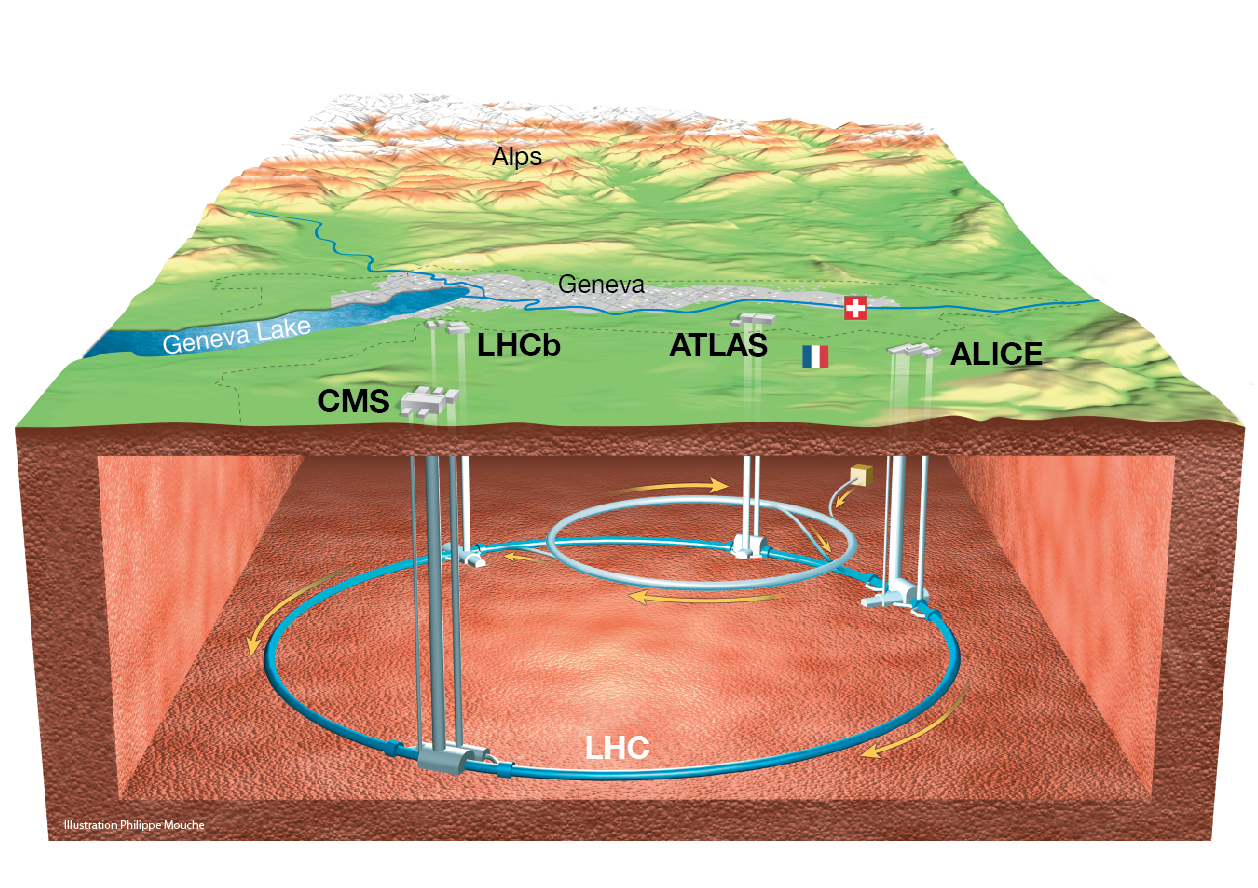
\includegraphics[width=0.75\linewidth]{plots/detector/LHC_overview.png}  \\
\caption[LHC overview]{The LHC and the four main experiments located at the four interaction regions.}
\label{fig:lhc-overview}
\end{figure}

The collider has four crossing points where the accelerated particles collide, as can be seen in the illustration in Figure~\ref{fig:lhc-overview}. Nine detectors have been constructed at the LHC, located underground in large caverns excavated at the LHC's intersection points. Two of them, the ATLAS experiment and \gls{cms}, are large general-purpose particle detectors. The other detectors have more specialized roles. ATLAS and CMS measure a variety of SM physics, such as Higgs boson and top quark production and look for BSM physics.

Two of the most interesting parameters of a particle collider are the center-of-mass energy of the collisions, and the luminosity. Due to energy conservation, the higher the energy of the collision, the heavier a theoretical particle can be produced. Therefore, in order to probe more massive theoretical particles (such as DM candidates in SUSY), the higher collision energy is necessary. The second parameter is the luminosity. The instantaneous luminosity depends on machine parameters, as was described in Section~\ref{sec:cross-section}, and is given by

\begin{equation}
\lumi=\frac{1}{\sigma} \dv{N}{t},
\end{equation}
where $\sigma$ is the corresponding cross section and $\ddinline{N}{t}$ is the rate of particle interactions. The integrated luminosity is given by integrating the instantaneous luminosity over a period of time
\begin{equation}
L=\int \lumi \dd t.
\end{equation}
The number of expected events N for a given process can be expressed in terms of the corresponding cross section $\sigma$ times the integrated luminosity $L$
\begin{equation}
N=L \cdot \sigma.
\end{equation}
Therefore, for rare processes, \ie, processes with very low cross section $\sigma$, access to large enough number of produced events requires higher integrated luminosity $L$. The integrated luminosity recorded in run 2 in CMS was around $138 \fbinv$.

\section{The Compact Muon Solenoid experiment}
\label{sec:cms}

The Compact Muon Solenoid (CMS) experiment is one of two large general-purpose particle physics detectors built on the Large Hadron Collider (LHC) at CERN in Switzerland and France, as previously mentioned. The CMS apparatus has an overall length of 22\unit{m}, a diameter of 15\unit{m}, and weighs 14\,000 \unit{tonnes}. The central feature of the CMS apparatus is a superconducting solenoid of 6\unit{m} internal diameter, providing a magnetic field of 3.8\unit{T}. Within the solenoid volume are a silicon pixel and strip tracker, a lead tungstate crystal electromagnetic calorimeter (ECAL), and a brass and scintillator hadron calorimeter (HCAL), each composed of a barrel and two endcap sections. Forward calorimeters extend the pseudorapidity coverage provided by the barrel and endcap detectors. Muons are measured in gas-ionization detectors embedded in the steel flux-return yoke outside the solenoid. A more detailed description of the CMS detector, together with a definition of the coordinate system used and the relevant kinematic variables, can be found in Ref.~\cite{CMS:2008xjf}. A cutaway diagram of the CMS detector can be seen in Figure~\ref{fig:cms-detector}.

\begin{figure}[!htb]
\centering
\includegraphics[width=0.85\linewidth]{plots/detector/cms_detector.pdf}  \\
\caption[A cutaway diagram of the CMS detector]{A cutaway diagram of the CMS detector.}
\label{fig:cms-detector}
\end{figure}

Events of interest are selected using a two-tiered trigger system. The first level (L1), composed of custom hardware processors, uses information from the calorimeters and muon detectors to select events at a rate of around 100\unit{kHz} within a fixed latency of about 4\mus~\cite{CMS:2020cmk}. The second level, known as the high-level trigger (HLT), consists of a farm of processors running a version of the full event reconstruction software optimized for fast processing, and reduces the event rate to around 1\unit{kHz} before data storage~\cite{CMS:2016ngn}.

The global event reconstruction (also called particle-flow event reconstruction~\cite{CMS:2017yfk}) aims to reconstruct and identify each individual particle in an event, with an optimized combination of all subdetector information. In this process, the identification of the particle type (photon, electron, muon, charged hadron, neutral hadron) plays an important role in the determination of the particle direction and energy. Photons (\eg coming from decays such as $\HGG$ or from electron bremsstrahlung) are identified as ECAL energy clusters not linked to the extrapolation of any charged particle trajectory to the ECAL. Electrons (\eg coming from $\PZ\rightarrow\Pep\Pem$ or $\PW\rightarrow\Pe\PAGne$) are identified as a charged particle track and potentially many ECAL energy clusters corresponding to this track extrapolation to the ECAL and to possible bremsstrahlung photons emitted along the way through the tracker material. Muons (\eg from $\PZ\rightarrow\PGmp\PGmm$ or $\PW\rightarrow\PGm\PAGnGm$) are identified as tracks in the central tracker consistent with either a track or several hits in the muon system, and associated with calorimeter deposits compatible with the muon hypothesis. Charged hadrons are identified as charged particle tracks neither identified as electrons, nor as muons. Finally, neutral hadrons are identified as HCAL energy clusters not linked to any charged hadron trajectory, or as a combined ECAL and HCAL energy excess with respect to the expected charged hadron energy deposit.

The energy of photons is obtained from the ECAL measurement. The energy of electrons is determined from a combination of the track momentum at the main interaction vertex, the corresponding ECAL cluster energy, and the energy sum of all bremsstrahlung photons attached to the track. The energy of muons is obtained from the corresponding track momentum. The energy of charged hadrons is determined from a combination of the track momentum and the corresponding ECAL and HCAL energies, corrected for the response function of the calorimeters to hadronic showers. Finally, the energy of neutral hadrons is obtained from the corresponding corrected ECAL and HCAL energies.

Jets are reconstructed offline all particle flow objects, clustered using the anti-\kt algorithm~\cite{Cacciari:2008gp, Cacciari:2011ma} with a distance parameter of 0.4. The raw jet energies are then corrected to establish a relative uniform response of the calorimeter in $\eta$ and a calibrated absolute response in transverse momentum \pt.

The primary vertex (PV) is taken to be the vertex corresponding to the hardest scattering in the event, evaluated using tracking information alone, as described in Section 9.4.1 of Ref.~\cite{CMS-TDR-15-02}. The missing transverse momentum vector \ptvecmiss is computed as the negative vector sum of the transverse momenta of all the PF candidates in an event, and its magnitude is denoted as \ptmiss~\cite{CMS:2019ctu}. The \ptvecmiss is modified to account for corrections to the energy scale of the reconstructed jets in the event.

The silicon tracker used in 2016 measured charged particles within the range $\abs{\eta} < 2.5$. For nonisolated particles of $1 < \pt < 10\GeV$ and $\abs{\eta} < 1.4$, the track resolutions were typically 1.5\% in \pt and 25--90 (45--150)\mum in the transverse (longitudinal) impact parameter~\cite{CMS:2014pgm}. At the start of 2017, a new pixel detector was installed~\cite{Phase1Pixel}; the upgraded tracker measured particles up to $\abs{\eta} < 3.0$ with typical resolutions of 1.5\% in \pt and 20--75\mum in the transverse impact parameter~\cite{DP-2020-049} for nonisolated particles of $1 < \pt < 10\GeV$.

Muons are measured in the pseudorapidity range $\abs{\eta} < 2.4$, with detection planes made using three technologies: drift tubes, cathode strip chambers, and resistive plate chambers. The single muon trigger efficiency exceeds 90\% over the full $\eta$ range, and the efficiency to reconstruct and identify high momentum muons is greater than 96\%. Matching muons to tracks measured in the silicon tracker results in a relative transverse momentum resolution, for muons with \pt up to 100\GeV, of 1\% in the barrel and 3\% in the endcaps. The \pt resolution in the barrel is better than 7\% for muons with \pt up to 1\TeV~\cite{CMS:2018rym}.


The integrated luminosities for the 2016, 2017, and 2018 data-taking years have 1.2--2.5\% individual uncertainties~\cite{CMS-LUM-17-003,CMS-PAS-LUM-17-004,CMS-PAS-LUM-18-002}, while the overall uncertainty for the 2016--2018 period is 1.6\%.


\chapter{Search for compressed Higgsinos  with soft lepton tracks}

\section{Motivation}
\section{Signal models}

The signal models considered in this analysis are based on  \fxnote{fill in signal model stuff}.

\begin{figure}[h]
\centering
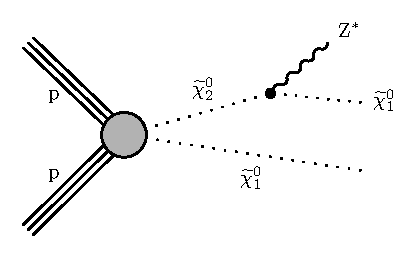
\includegraphics[width=0.48\linewidth]{plots/feynman_diagrams/gitTChiZ.pdf} \,
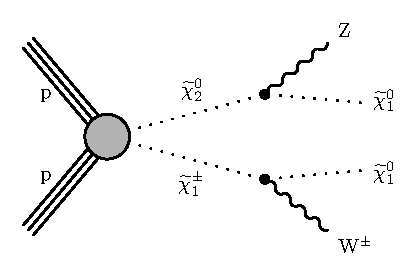
\includegraphics[width=0.48\linewidth]{plots/feynman_diagrams/gitTChiWZ.pdf}  \\
\caption[Signal Models Feynman Diagrams]{Production and decay of electroweakinos in the higgsino simplified model through \tchiz (left) and \tchiwz (right). }
\label{fig:signal-feynman-diagrams}
\end{figure}


\section{Previous searches}
\clearpage
\section{Search strategy}
\label{sec:search-strategy}

The search details are described in depth in the upcoming sections. However, it is useful to have a very quick overview of the strategy so that it is easier to follow. This analysis targets the two leptons resulting from the decay of the \neutt. Those are opposite-charge, same-flavor leptons \ellell resulting from the \neutt that decays into a \neuto and a \PZstar, \ie, \neuttdecay. If there is a \chargino present, such as in the production of \tchiwz, it is assumed to either decay hadronically or that the resulting lepton is not identified. The invariant mass of the two leptons resulting from the decay has a unique shape due to the limited allowed phase space of the 3-body decay and is restricted to the mass difference between \neutt and \neuto, that is, \dm. Therefore, the $\mll$ distribution is expected to have an edge at \dm. The presence of two \neuto in the final state, lead to high \MET in the event, which leads to the use of triggers based on missing transverse energy. Typical for such topographies, an ISR jet is also required for increased sensitivity.

The analysis has three channels which correspond to two physical final states: two identified muons, one identified muon and one track, and one identified electron and one track. The channels with one identified lepton and one track result from one of the leptons not being identified due to the low identification efficiency for low momentum objects. There is no channel corresponding to two identified electrons, since that has been analyzed already in the SOS paper~\cite{sos}. All channels utilizes a BDT in order to select signal and reject SM background. The BDT discriminator outputs are also used to define the signal regions for signal extraction and limit settings, as well as control regions for background estimation purposes. The identified lepton plus track channels utilize an addition object level BDT discriminator in order to select a track among the collection of tracks in an event, which hopefully corresponds to the non-identified lepton. The key points of each channel are summarized in the sections bellow.


\subsection{Final state with two identified muons}
\label{sec:dimuon-category}

\begin{itemize}
\item \textbf{Defining objects:} two identified opposite-charge muons.
\item \textbf{Signal regions:} using bins in an event BDT score of $\text{BDT}>0$.
\item \textbf{Background estimation:} isolated background arising from leptonic decays of $\tau\tau$ is estimated using MC, and non-isolated background is estimated using dedicated isolation sideband CR in data.

\end{itemize}

\subsection{Final state with one identified lepton and one track}
\label{sec:exclusive-track-category}

\begin{itemize}
\item \textbf{Defining objects:} one identified lepton (muon or electron) and one opposite charge track having maximum track picking BDT score.
\item \textbf{Signal regions:} using bins in an event BDT score of $\text{BDT}>0$.
\item \textbf{Background estimation:} using same-sign CR in data.
\end{itemize}

\clearpage
\section{Signal signature and base selection}
\label{sec:signal-signature}

To develop an effective analysis strategy, one must study and exploit the signal kinematics. The production of electroweakinos has unique characteristics that can be leveraged to differentiate the signal from the \gls{sm} background. It is crucial to examine these signal distributions to define a preselection or base cut that retains the maximum signal while rejecting as much background as possible. All the following distributions were generated by weighting the simulation to the Run II luminosity of $\lumi = 135 \fbinv$ and requiring at least one jet in the event with $\pt \geq 30\GeV$ and $\abs{\eta}<2.4$. Any additional selection criteria will be listed in each section, if applicable.

\subsection{Missing Transverse Energy}
\label{subsec:signal-met-mht}

A common property shared by essentially all searches for \gls{dam} is the presence of a \gls{dam} candidate in the production. The identity and properties of the particle (or particles in the case of multiple \gls{dam} candidates) vary, but they do have much in common. In this \gls{susy} search, the \gls{neutralino} is the \gls{dam} candidate, which is a type of \gls{wimp}. A \gls{wimp} is a new elementary particle that interacts via gravity and potentially other forces, not part of the \gls{sm} itself, and is as weak as or weaker than the weak nuclear force, but also non-vanishing in strength. This essentially means that such a candidate is neutral and does not interact via the electromagnetic force. A neutral particle that does not interact electromagnetically or via the strong force (\ie, is colorless) will not be detected and will leave traces in the form of a transverse momentum imbalance, which is referred to as \gls{met} (Missing Transverse Energy or Missing Transverse Momentum). The signal contains two \gls{dam} candidates in the production, which are the \glspl{lsp}, the \glspl{neutralino} \neuto. Therefore, a considerable magnitude of \gls{met} is expected in the signal. As described in Section~\ref{subsec:met}, \gls{mht} is of greater interest, which is highly correlated with \gls{met}, due to the definition of lepton isolation and its use in the background estimation methods. Nonetheless, both $\MET$ and $\mht$ observables will be examined in Figure~\ref{fig:signal-met-mht}.


\begin{figure}[!htb]
\centering
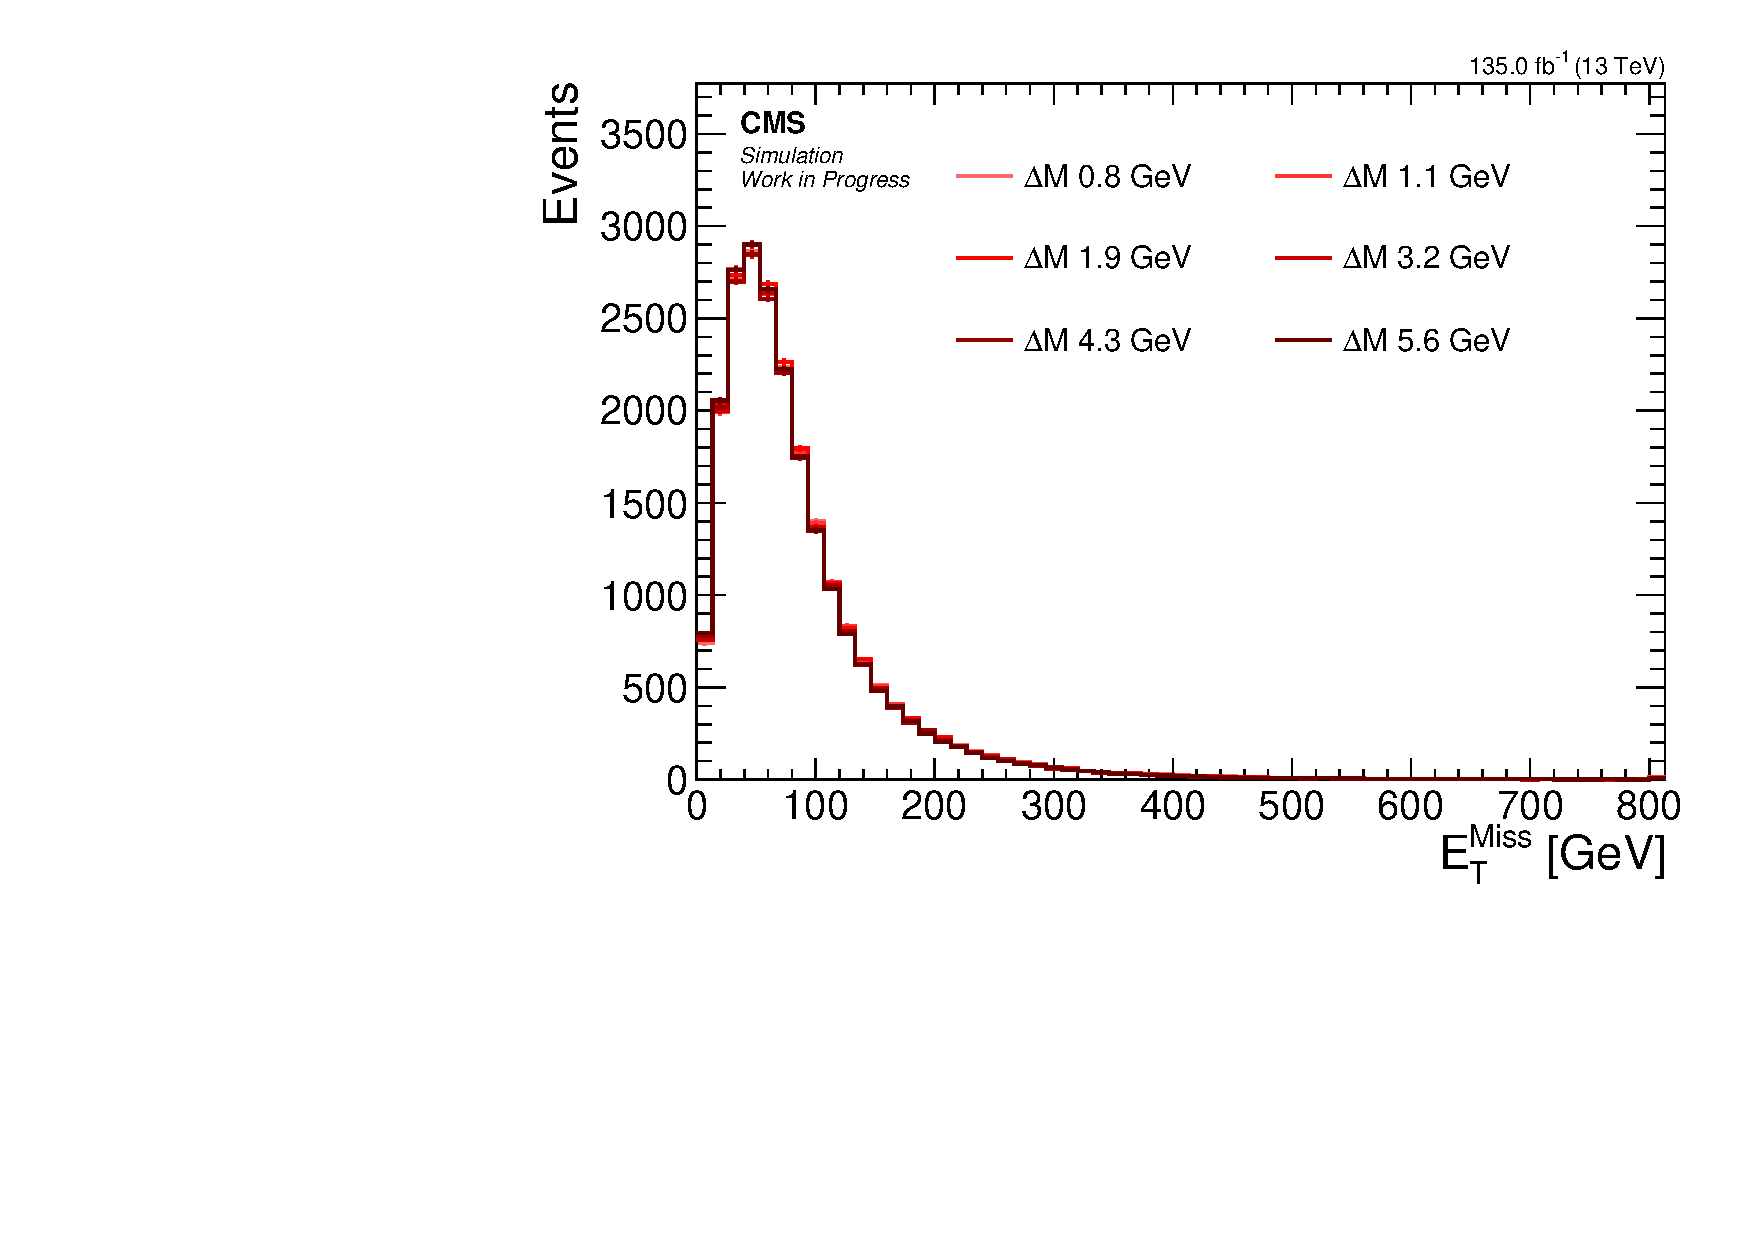
\includegraphics[width=0.48\linewidth]{plots/signal_common_distributions_fixed_mu/none_MET.pdf} \,
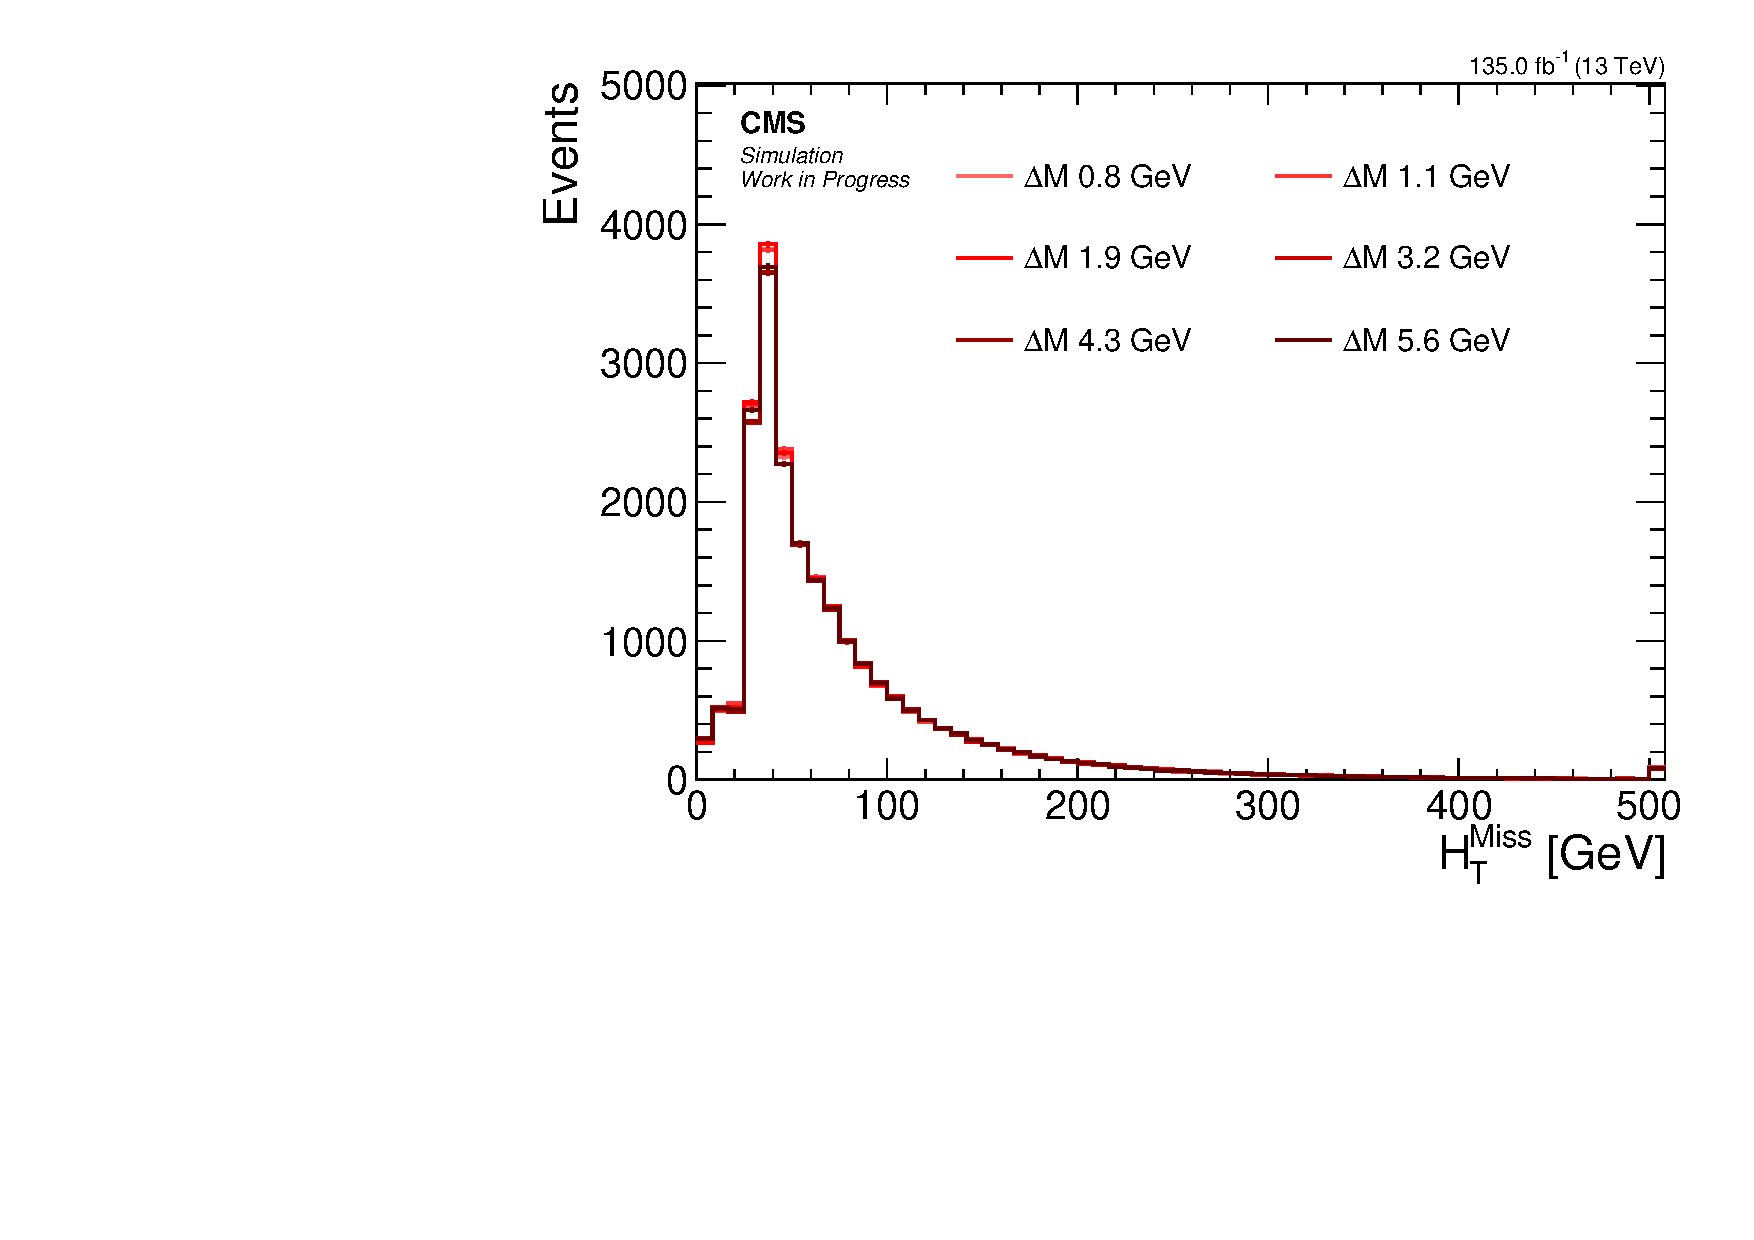
\includegraphics[width=0.48\linewidth]{plots/signal_common_distributions_fixed_mu/none_MHT.pdf}  \\
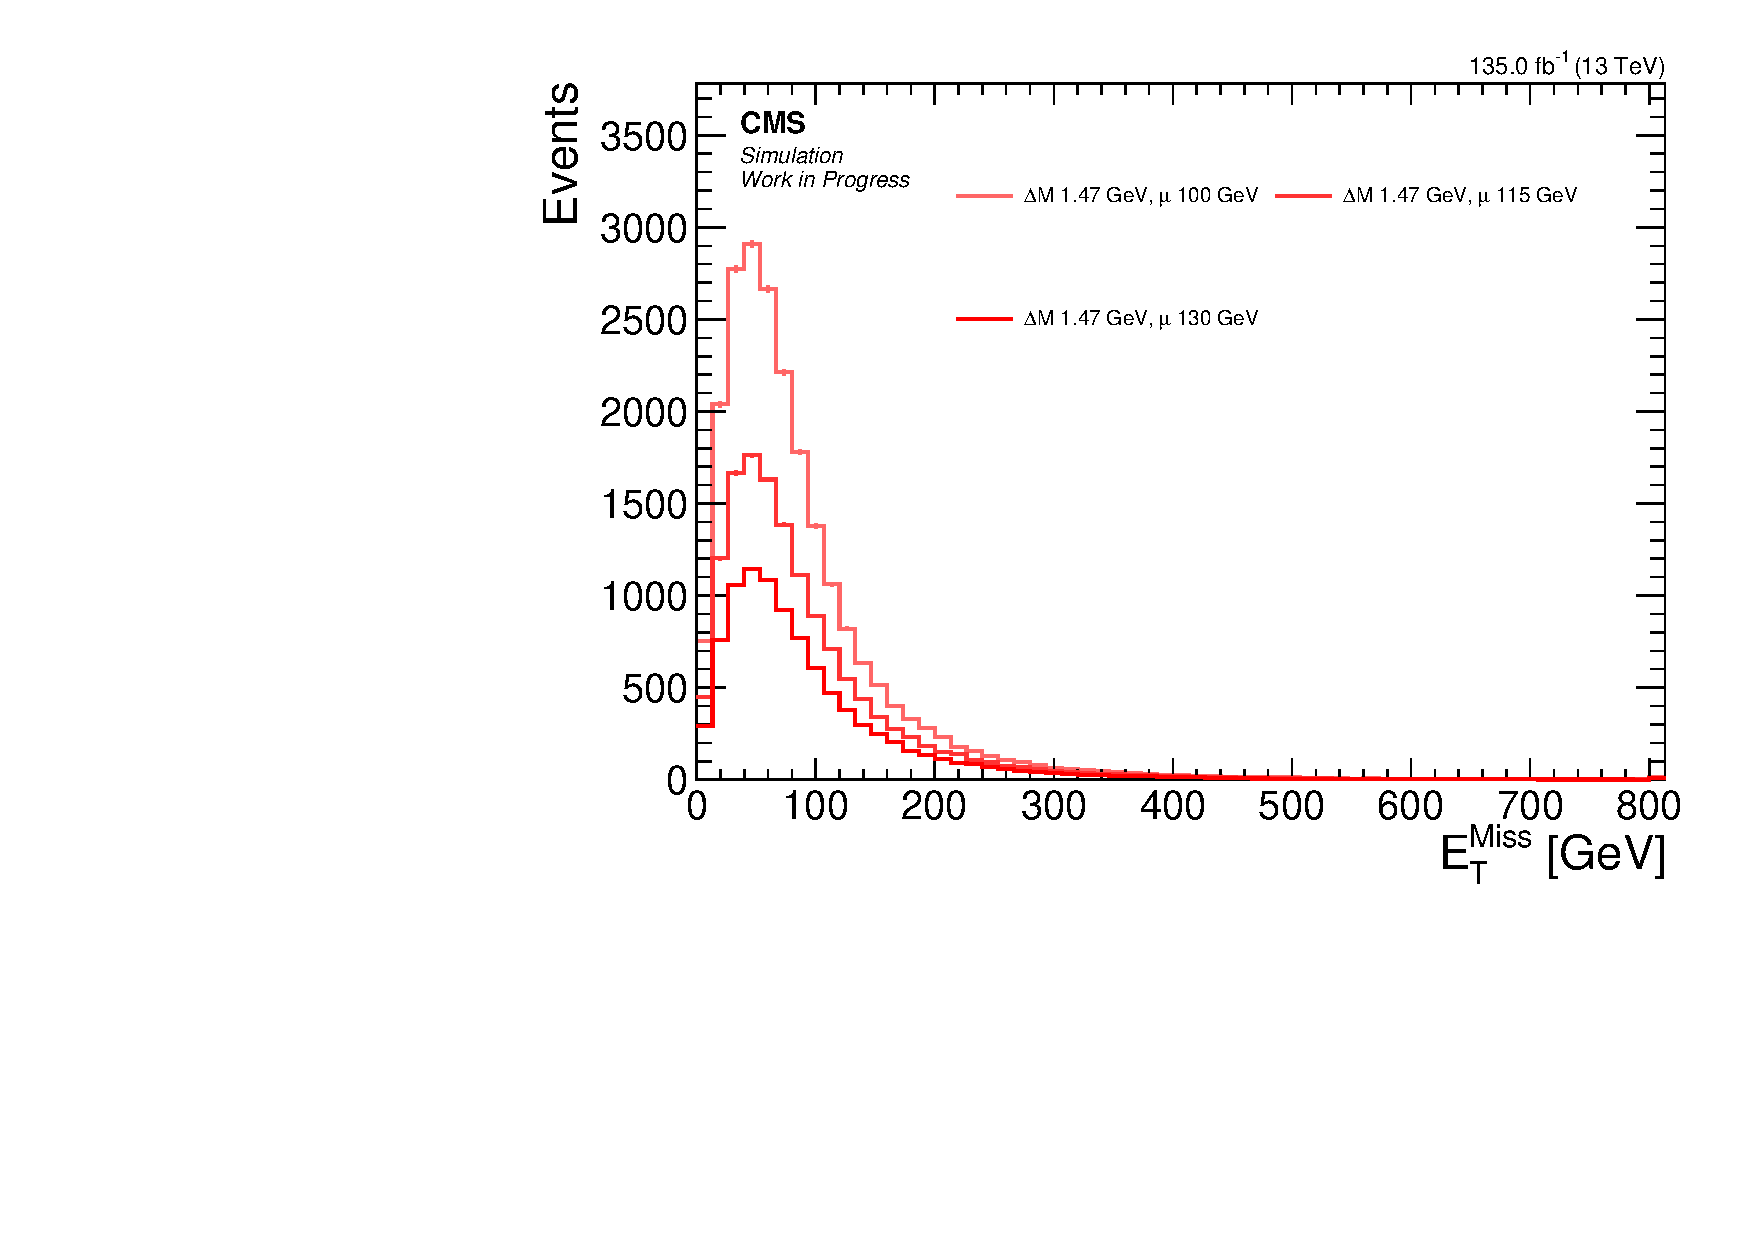
\includegraphics[width=0.48\linewidth]{plots/signal_common_distributions_fixed_dm/none_MET.pdf} \,
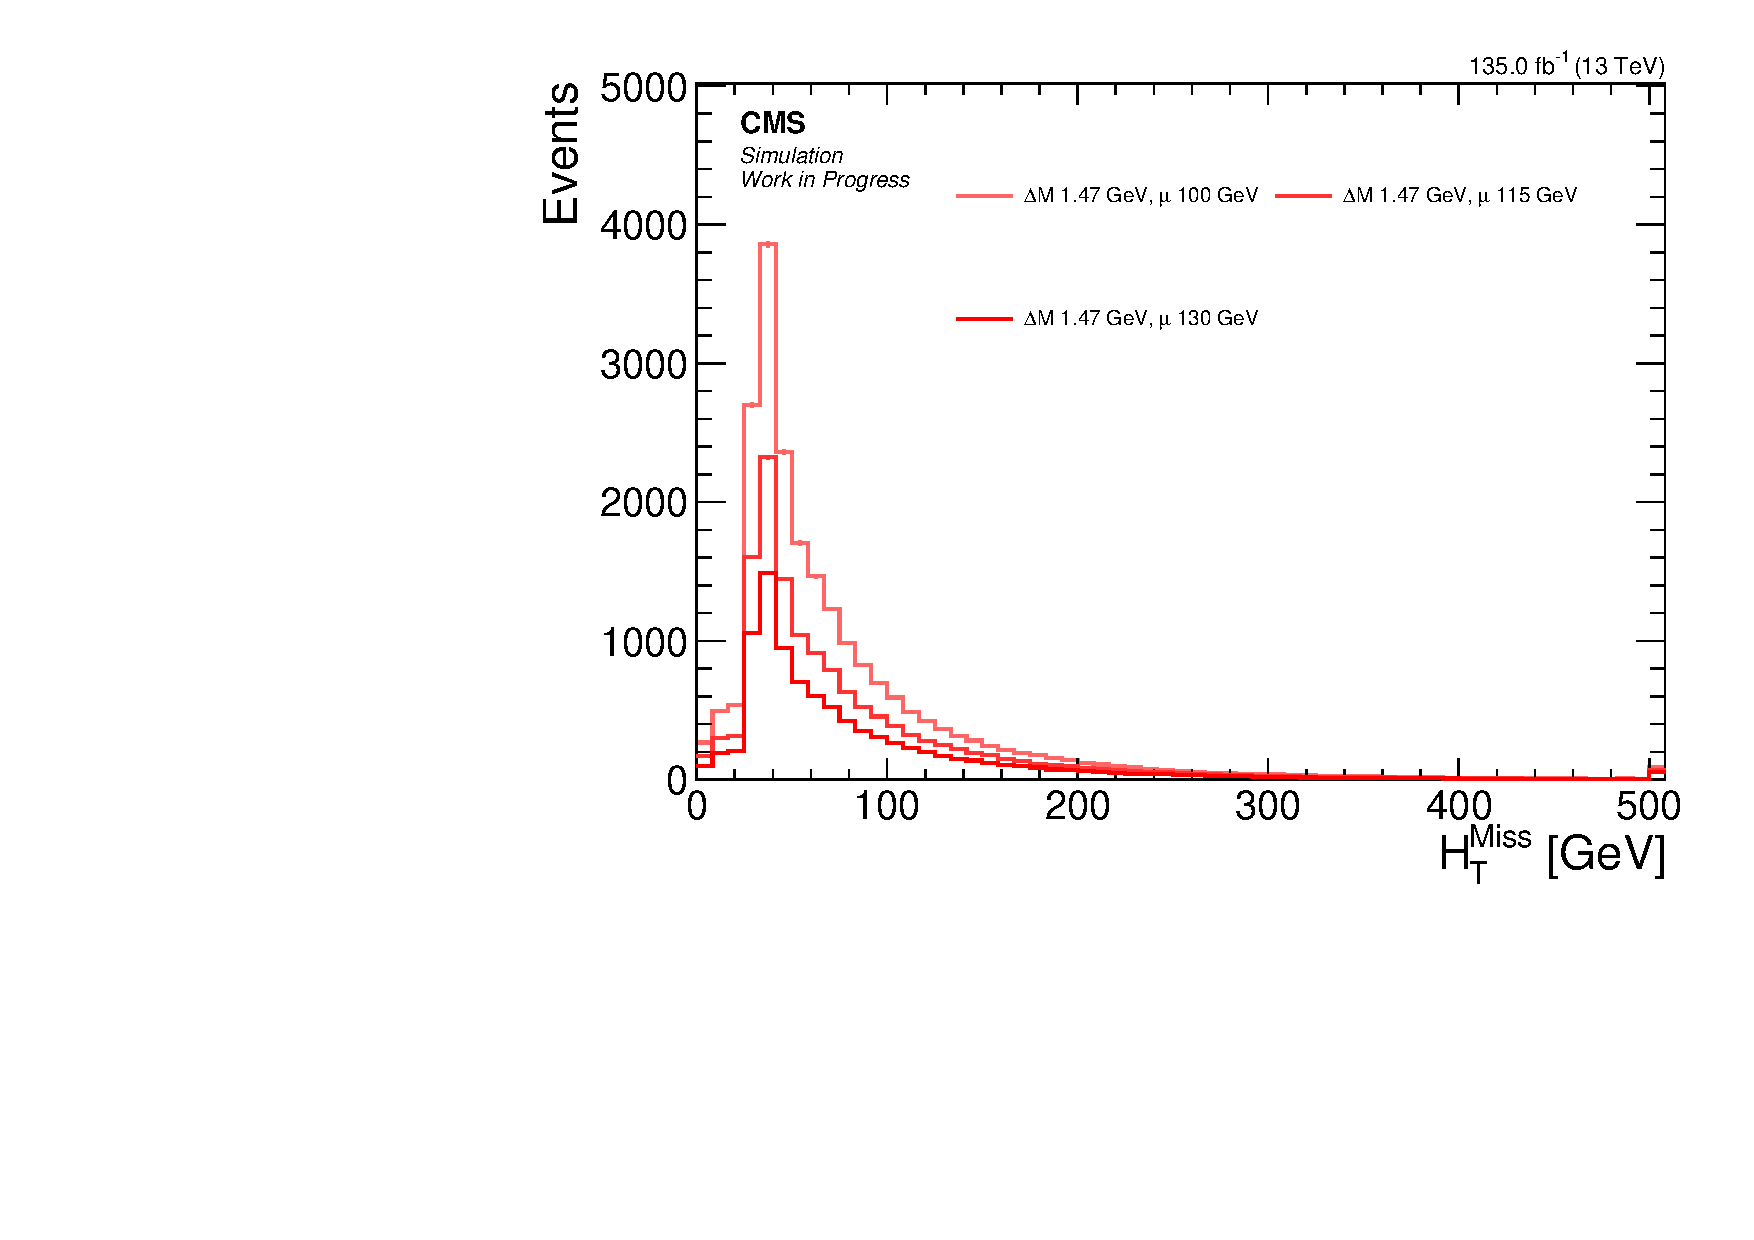
\includegraphics[width=0.48\linewidth]{plots/signal_common_distributions_fixed_dm/none_MHT.pdf}  \\
\caption[Signal $\MET$ and $\mht$ distributions]{ Signal distributions for \MET (left) and \mht (right) comparing various $\dm$ with a fixed higgsino parameter $\mu=100\GeV$ (upper), and comparing various higgsino parameters $\mu$ with fixed $\dm=1.47\GeV$ (lower).}
\label{fig:signal-met-mht}
\end{figure}

As expected, $\MET$ and $\mht$ are hardly affected by the different choices for \dm, while the higgsino parameter $\mu$ affects the distributions mainly through its lower production cross section for higher higgsino parameter $\mu$. The region of interest for triggering purposes is located at $\mht\geq 220$, as discussed in Section~\ref{sec:trigger}. Although this is a harsh and inefficient cut, it is necessary to consider the \gls{sm} background in both regions of $\mht < 220$ and $\mht\geq 220$ to conclude that most of the sensitivity comes from the $\mht\geq 220$ region, as the production of real \gls{mht} (or \gls{met}) results from the production of neutrinos in the event, which are much less common than \gls{qcd} events that dominate the $\mht < 220$ region. Therefore, a cut at $\mht\geq 220$ might be inefficient, but it results in high sensitivity.

\subsection{Jets and hardronic activity}

To maximize the boost of the \glspl{neutralino} \neuto that contribute to the \gls{mht} and drive sensitivity in the high \gls{mht} region, it is desirable to maximize their transverse momentum \gls{pt}. A widely used method is to include an \gls{isr} jet in the event. An \gls{isr} jet is created when one of the incoming protons emits radiation (such as a photon or a gluon) before the interaction. If a jet with sufficiently high \gls{pt} is emitted, the remainder of the interaction is recoiled against this jet and imparts momentum to it in the opposite direction. As a result, the boosted \glspl{neutralino} \neuto will have higher \gls{mht}. As described in Section~\ref{subsec:jets}, the jets are required to have $\pt \geq 30\GeV$ and be located within the tracker acceptance $\left(\abs{\eta}<2.4\right)$. At least one such jet is required in each event. The distributions of the number of jets and the leading jet \pt are displayed in Figure~\ref{fig:signal-njets-ljpt}.

\begin{figure}[!htb]
\centering
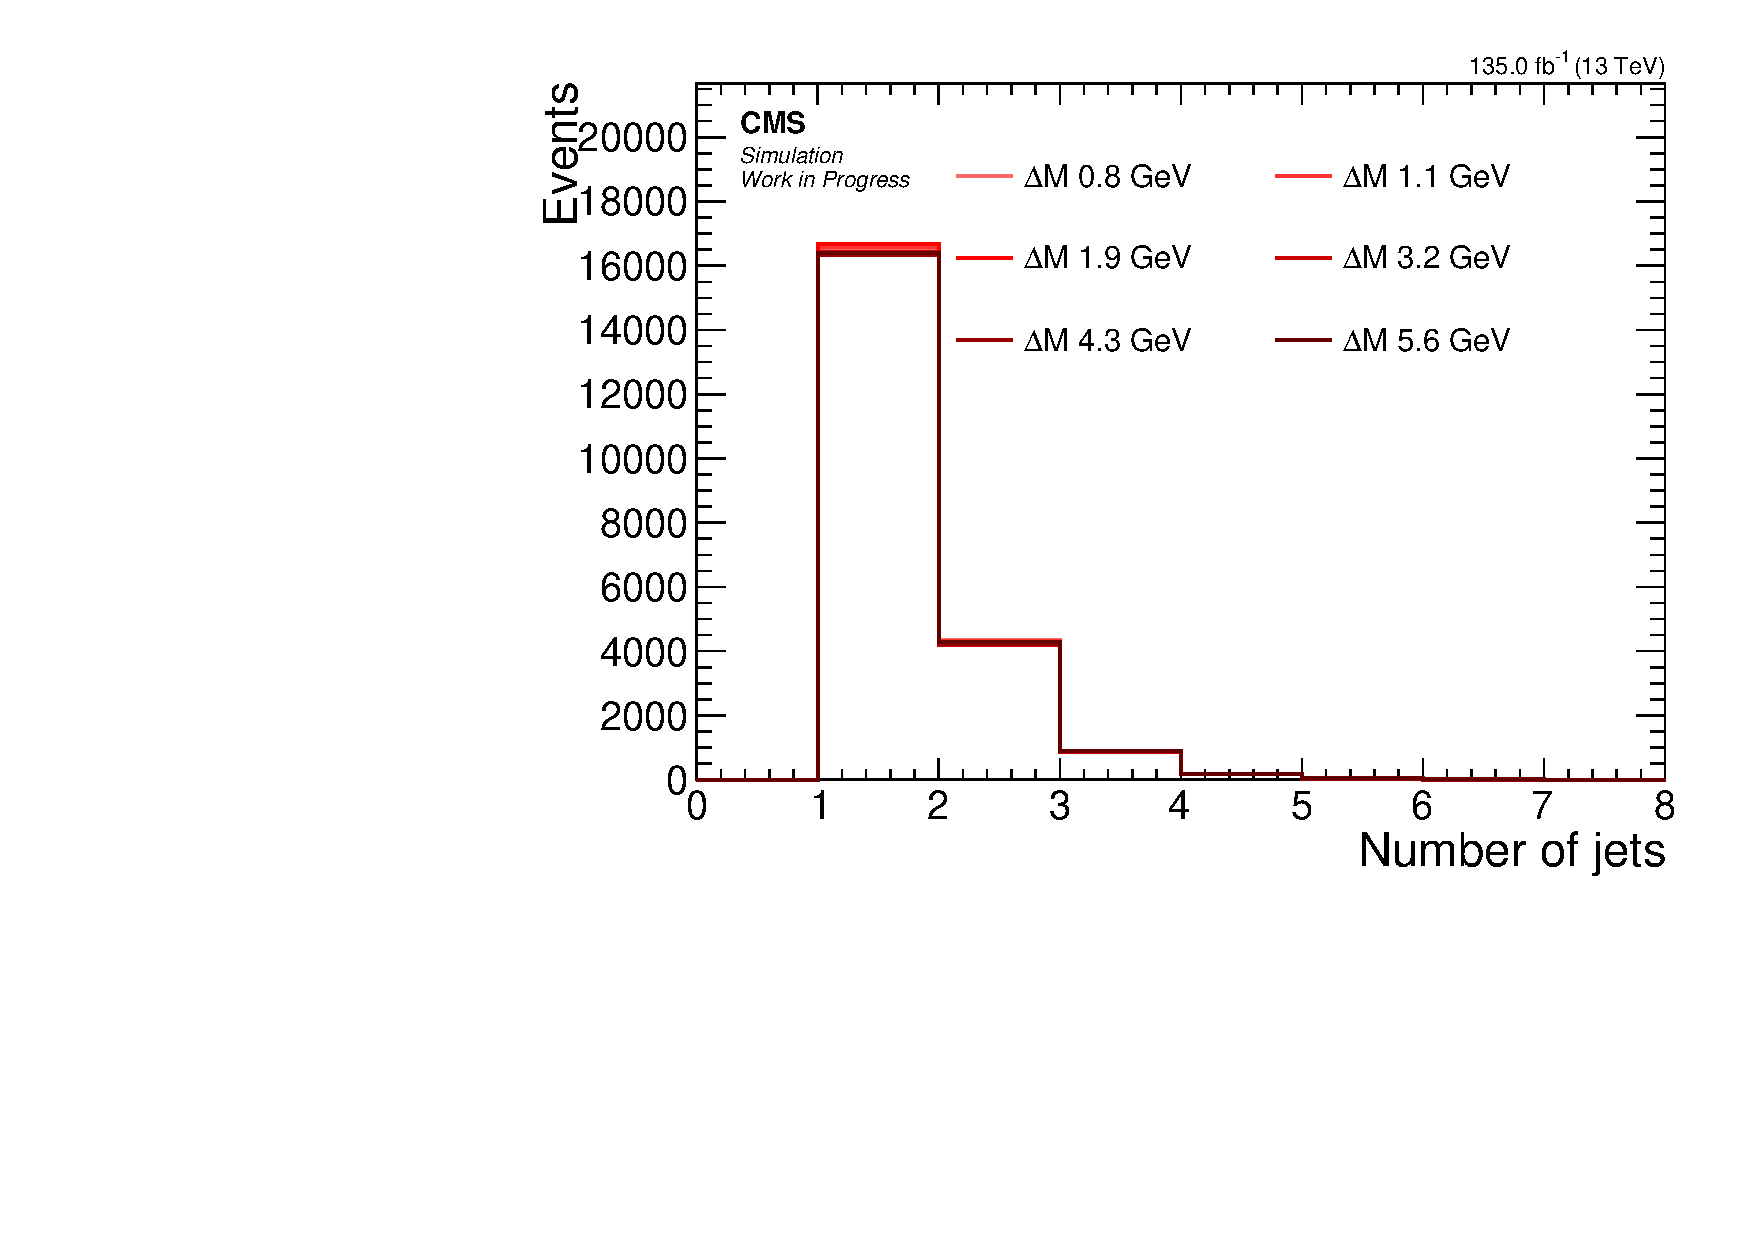
\includegraphics[width=0.48\linewidth]{plots/signal_common_distributions_fixed_mu/none_NJets.pdf} \,
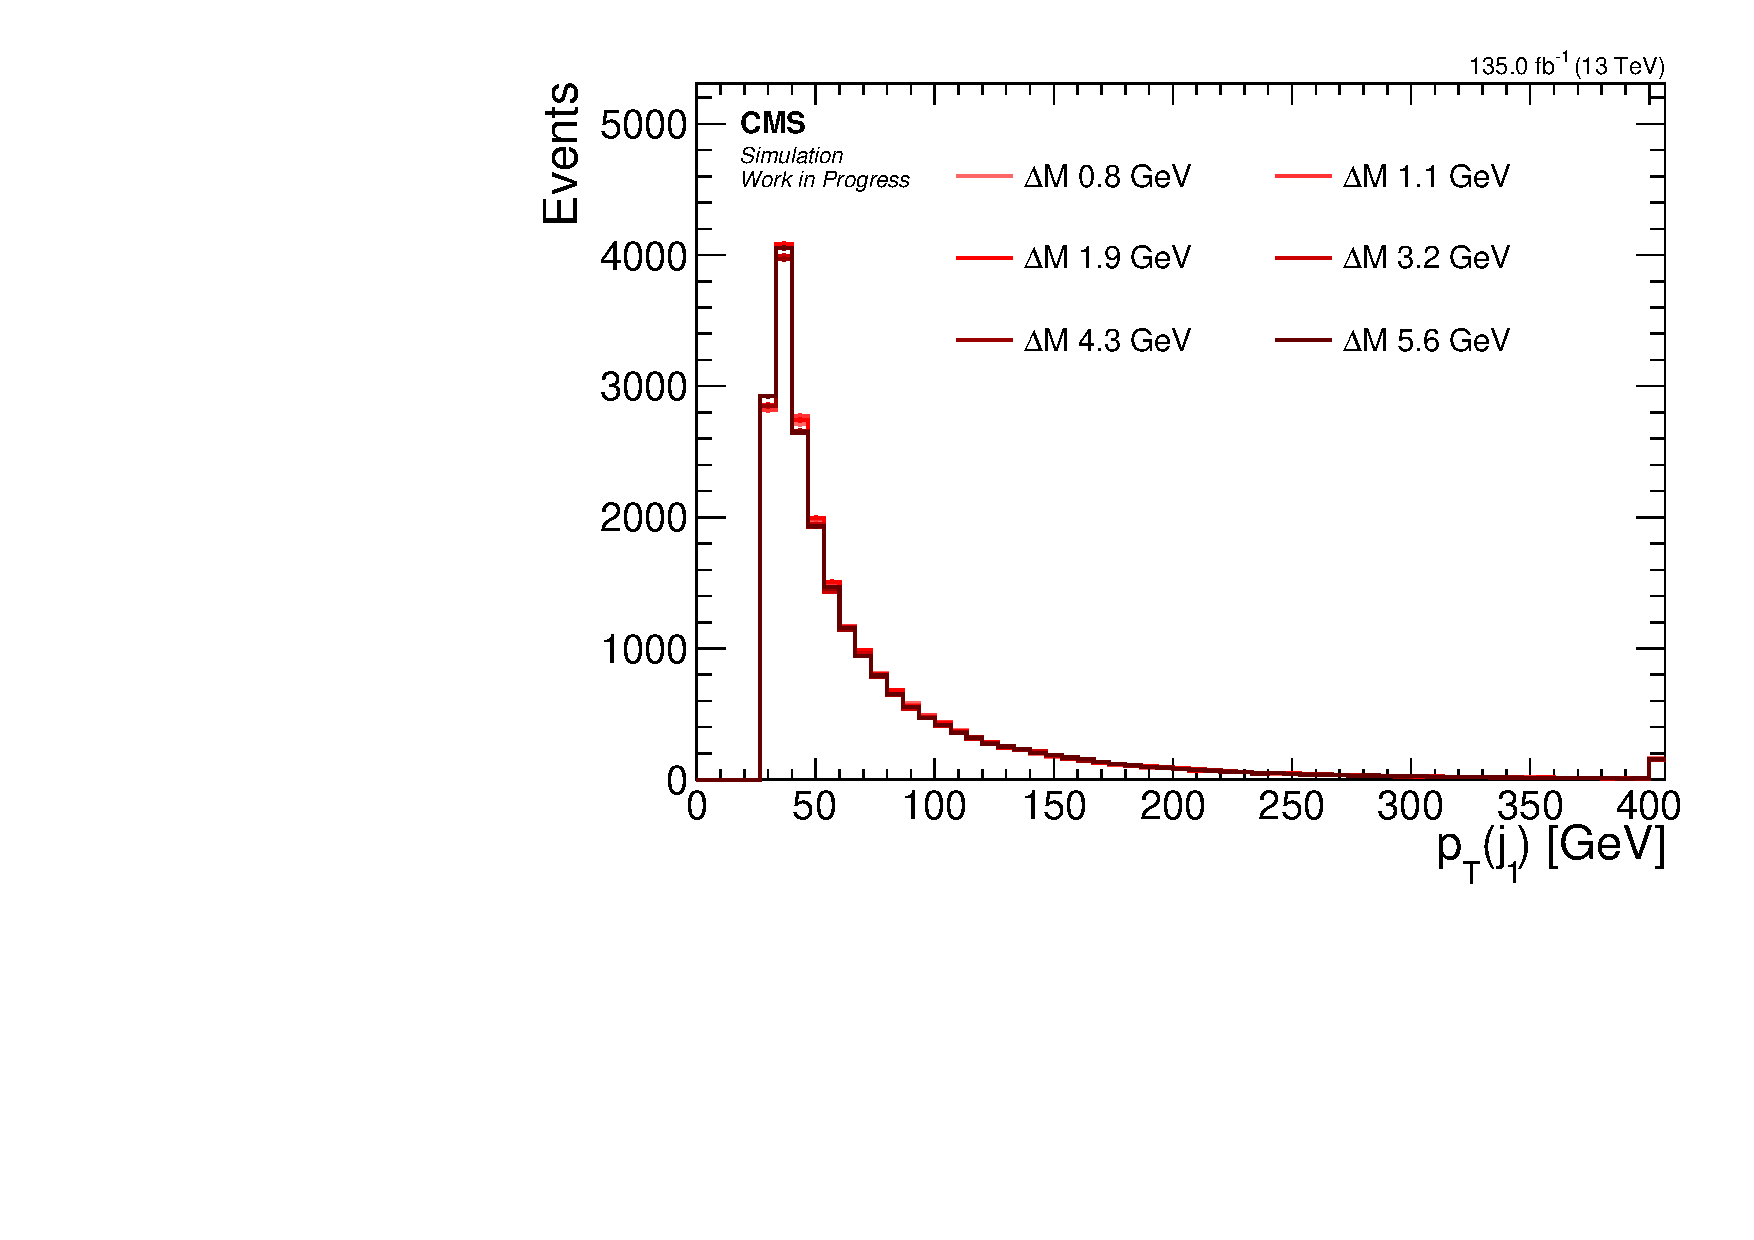
\includegraphics[width=0.48\linewidth]{plots/signal_common_distributions_fixed_mu/none_LeadingJetPt.pdf}  \\
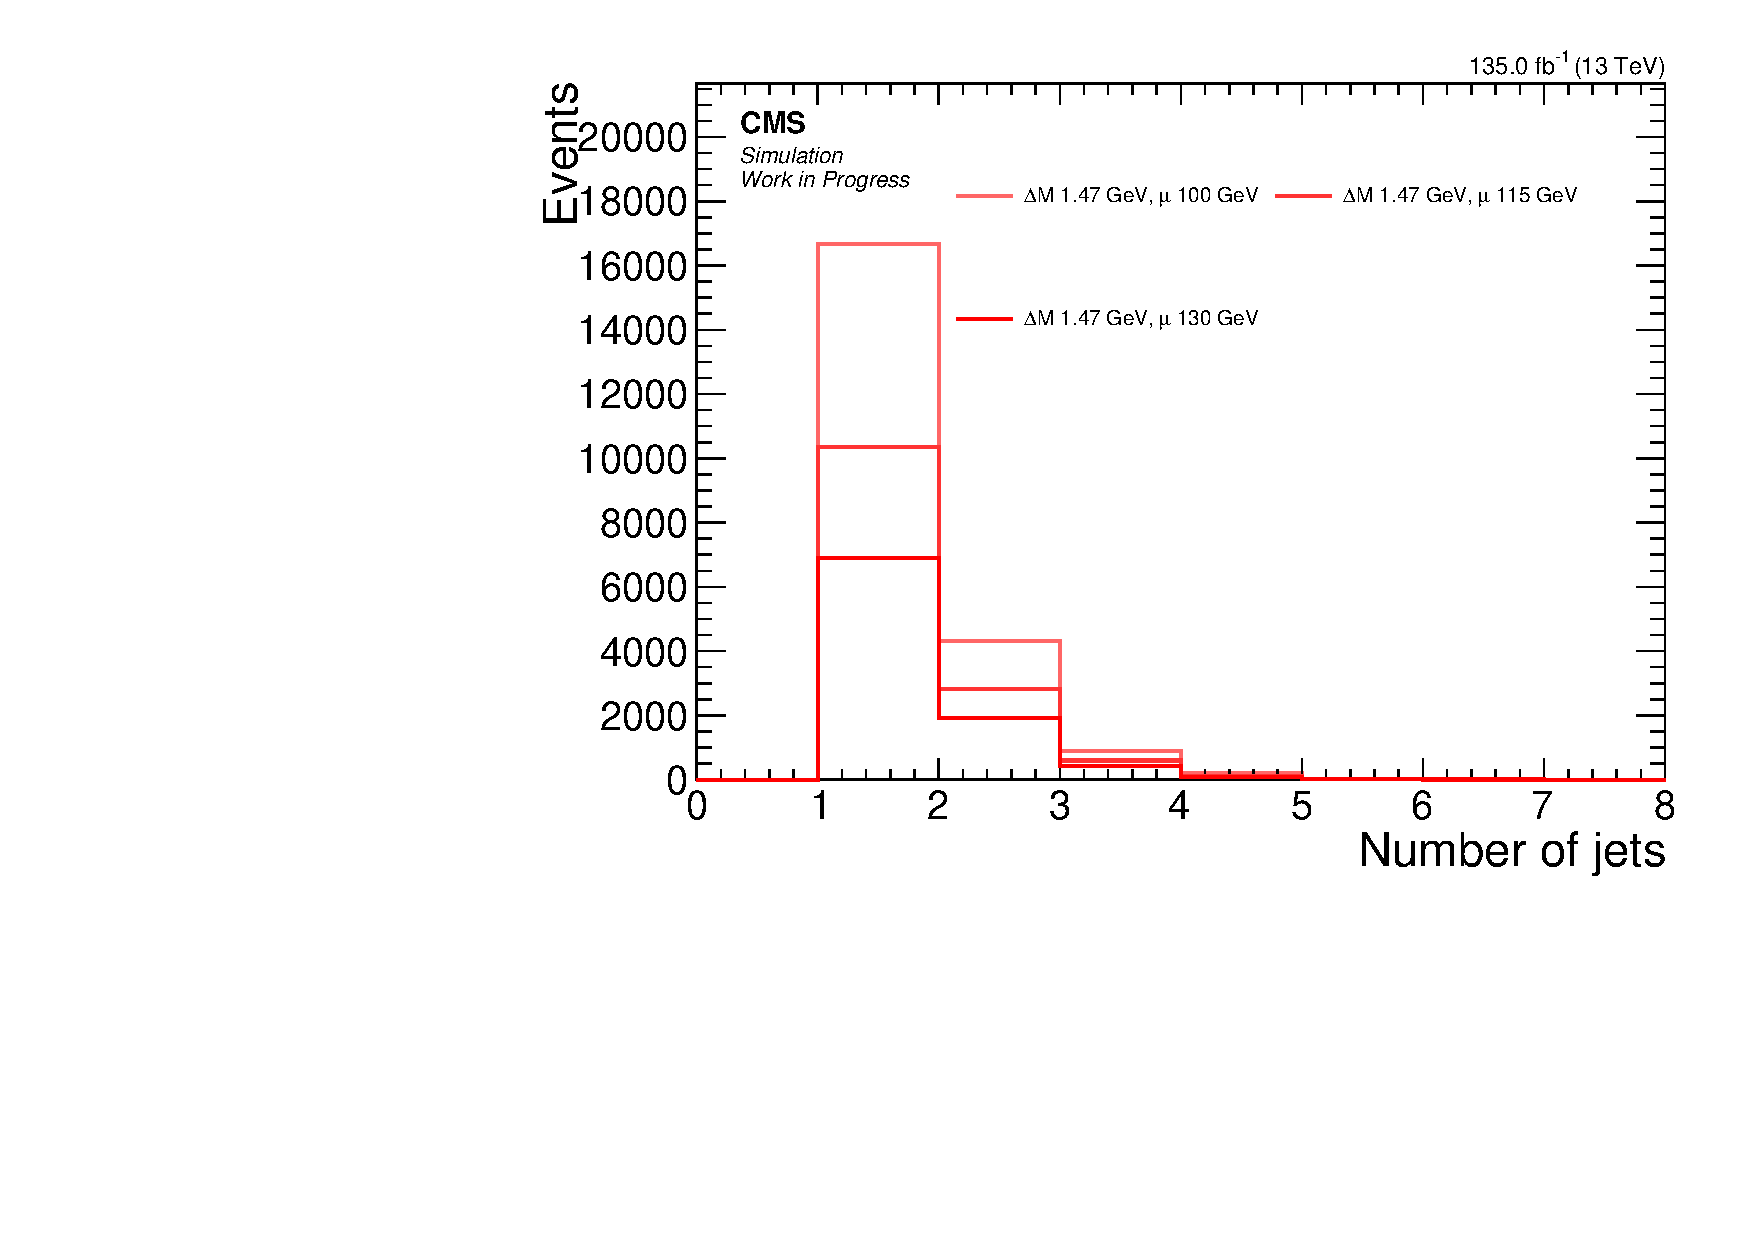
\includegraphics[width=0.48\linewidth]{plots/signal_common_distributions_fixed_dm/none_NJets.pdf} \,
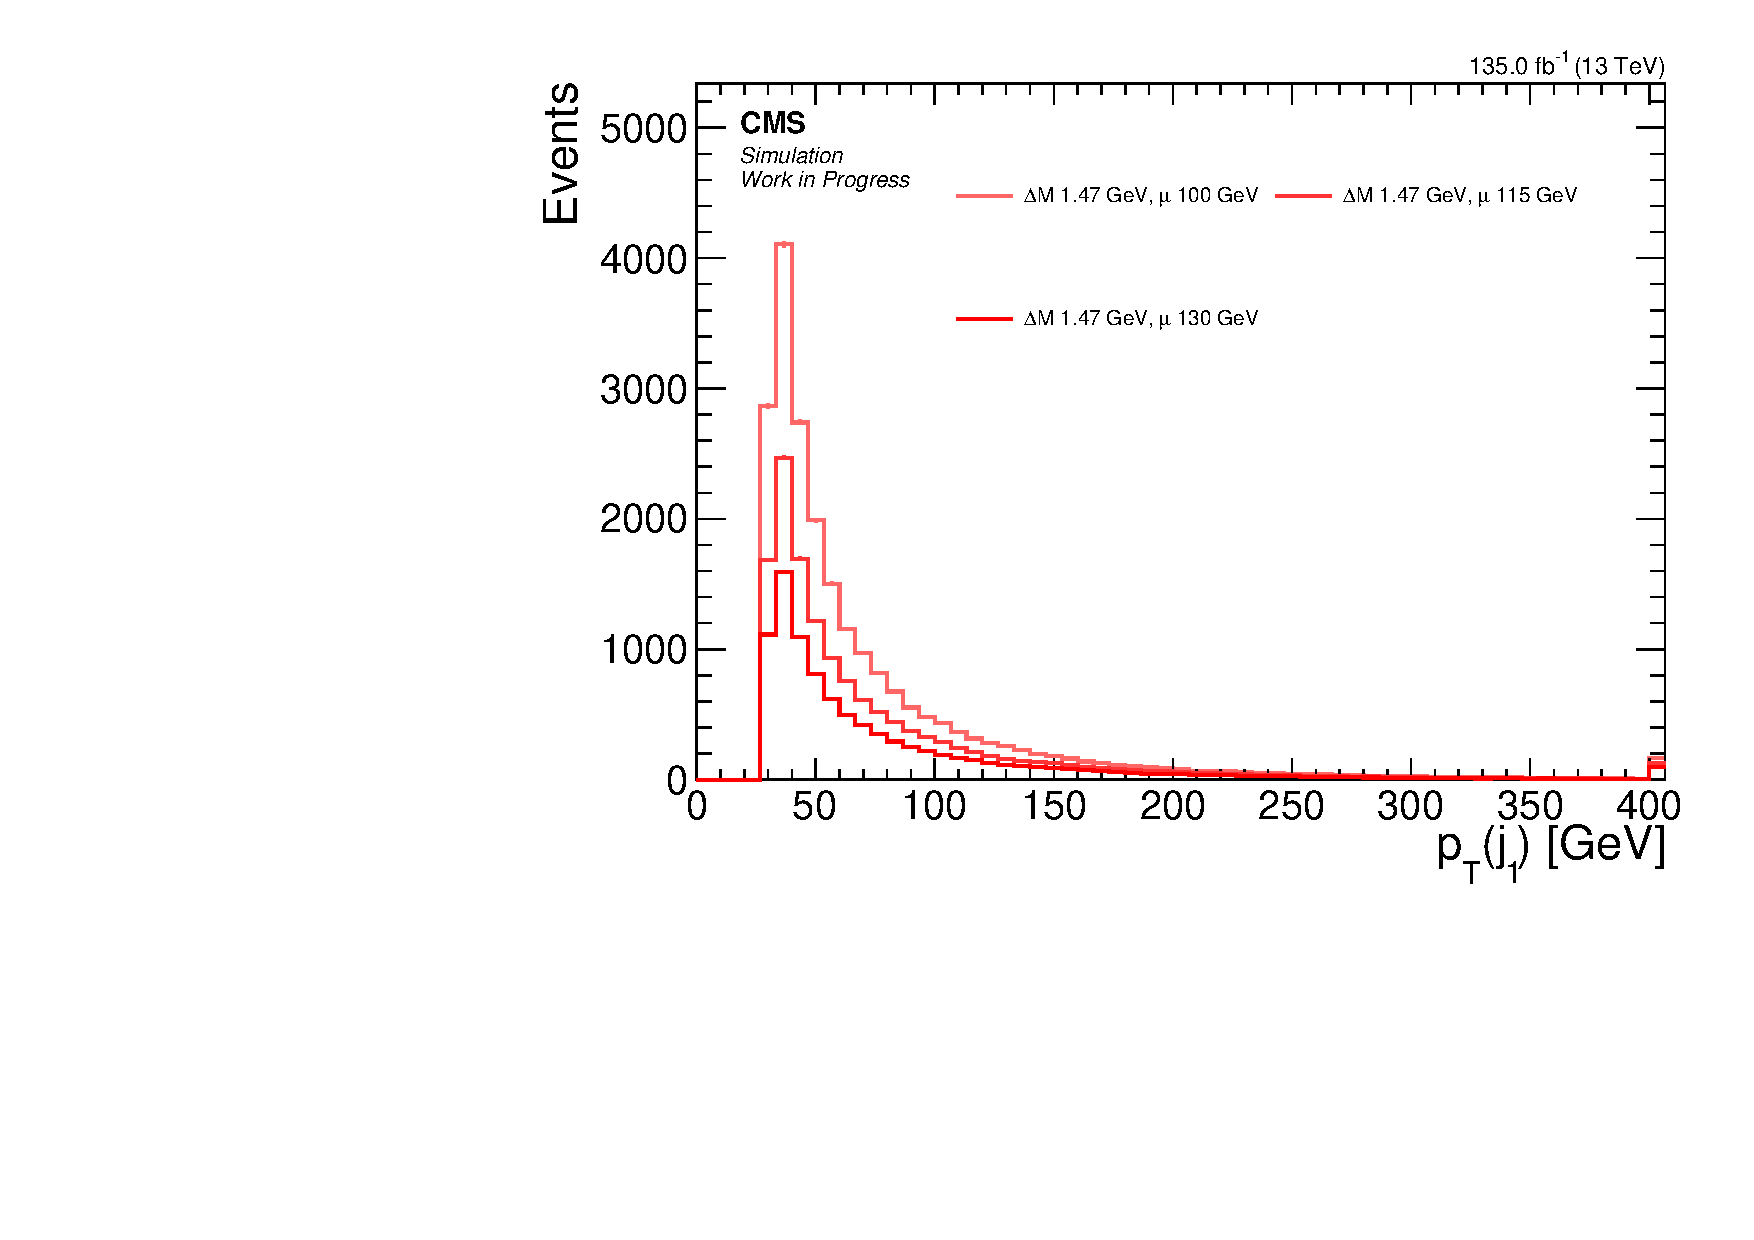
\includegraphics[width=0.48\linewidth]{plots/signal_common_distributions_fixed_dm/none_LeadingJetPt.pdf}  \\
\caption[Signal \emph{number of jets} and \emph{leading jet \pt} distributions]{ Signal distributions for \emph{number of jets} (left) and \emph{leading jet \pt} (right) comparing various $\dm$ with a fixed higgsino parameter $\mu=100\GeV$ (upper), and comparing various higgsino parameters $\mu$ with fixed $\dm=1.47\GeV$ (lower).}
\label{fig:signal-njets-ljpt}
\end{figure}

The signal signature does not include a \PQb-jet, that is, a jet resulting from a bottom quark hadronization (either resulting from a top quark or not). This knowledge is exploited by vetoing \PQb-tagged jets in the event. As described in Section~\ref{subsec:jets}, the \DEEPCSV bottom flavor tagging discriminant with a medium working point is used. The majority of the signal can be seen in the 0 bin, and thus any \PQb-tagged jet will be vetoed, retaining most of the signal but rejecting a lot of \gls{sm} background, such as that arising from \ttbar events.

\begin{figure}[!htb]
\centering
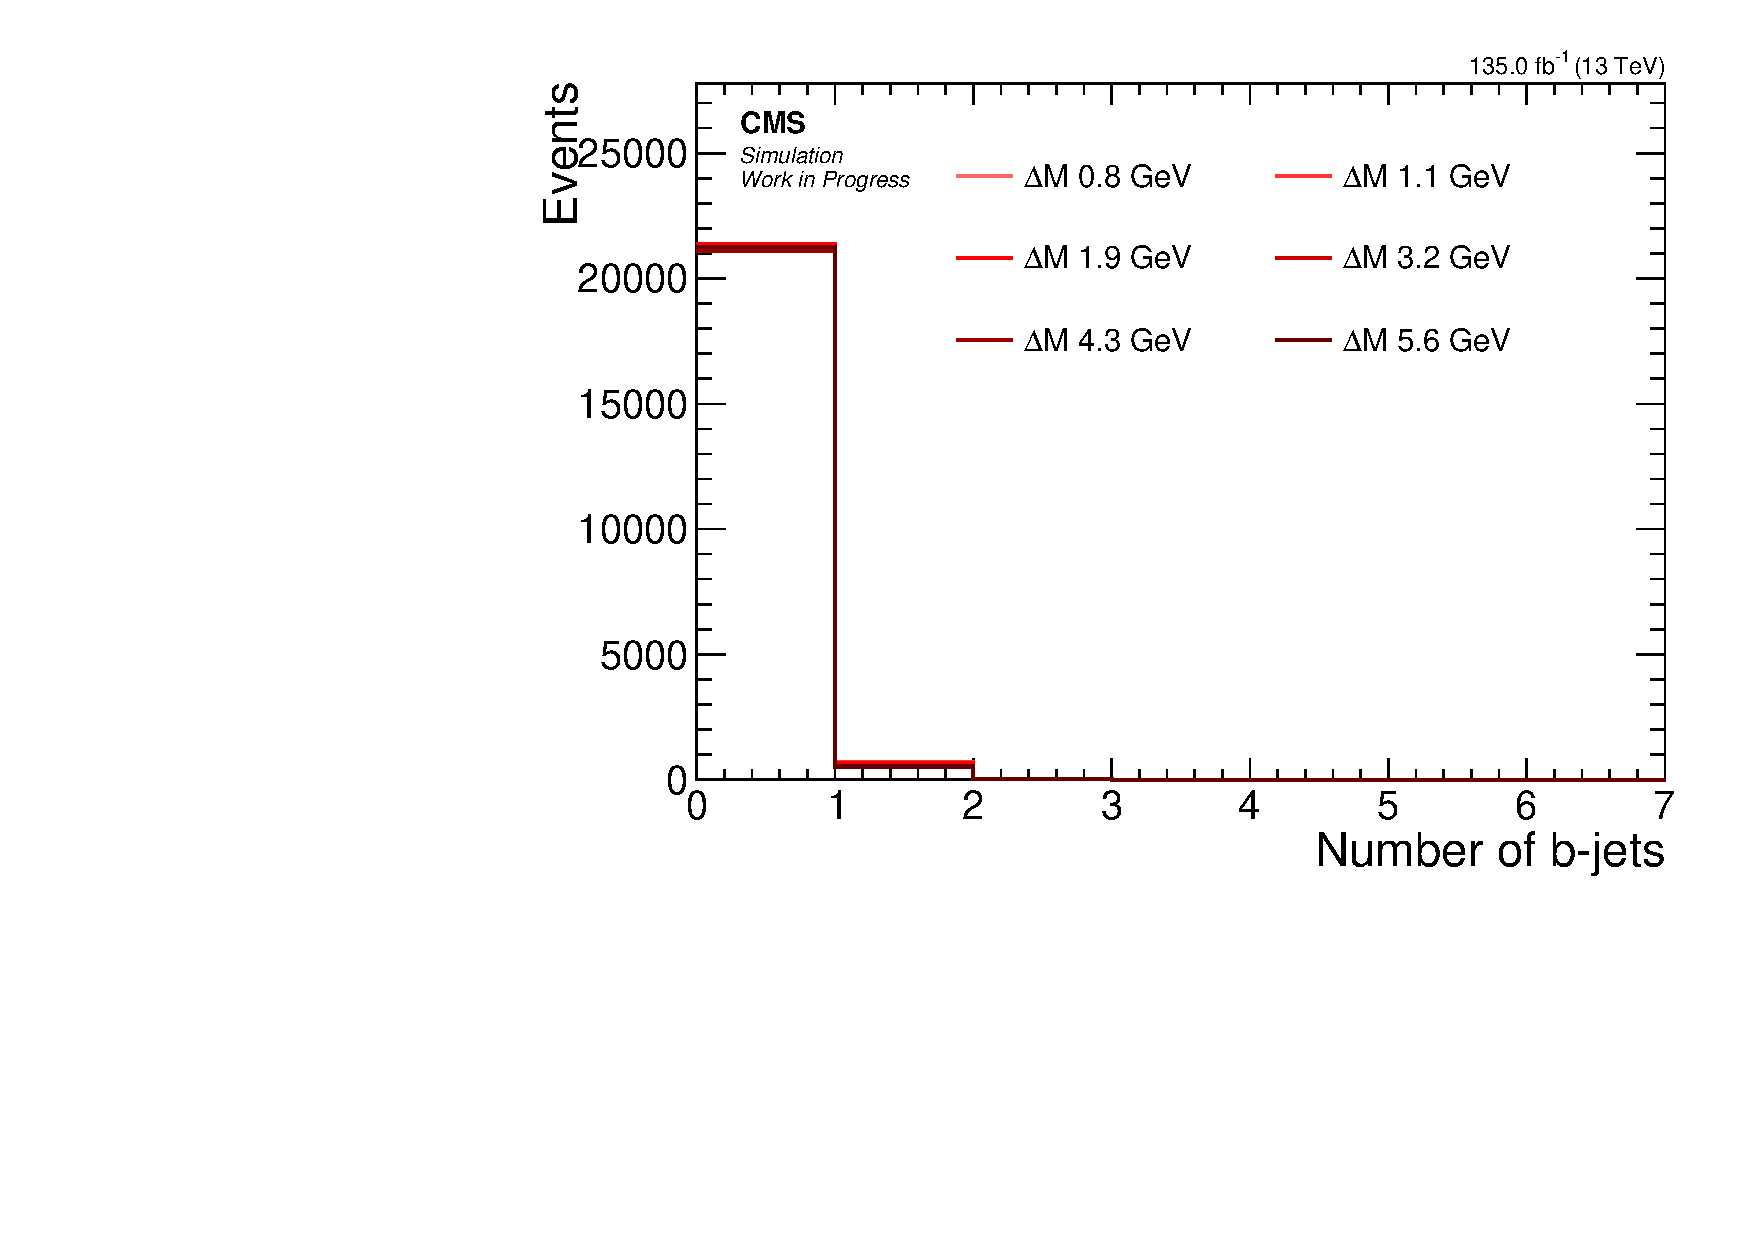
\includegraphics[width=0.48\linewidth]{plots/signal_common_distributions_fixed_mu/none_BTagsDeepMedium.pdf} \,
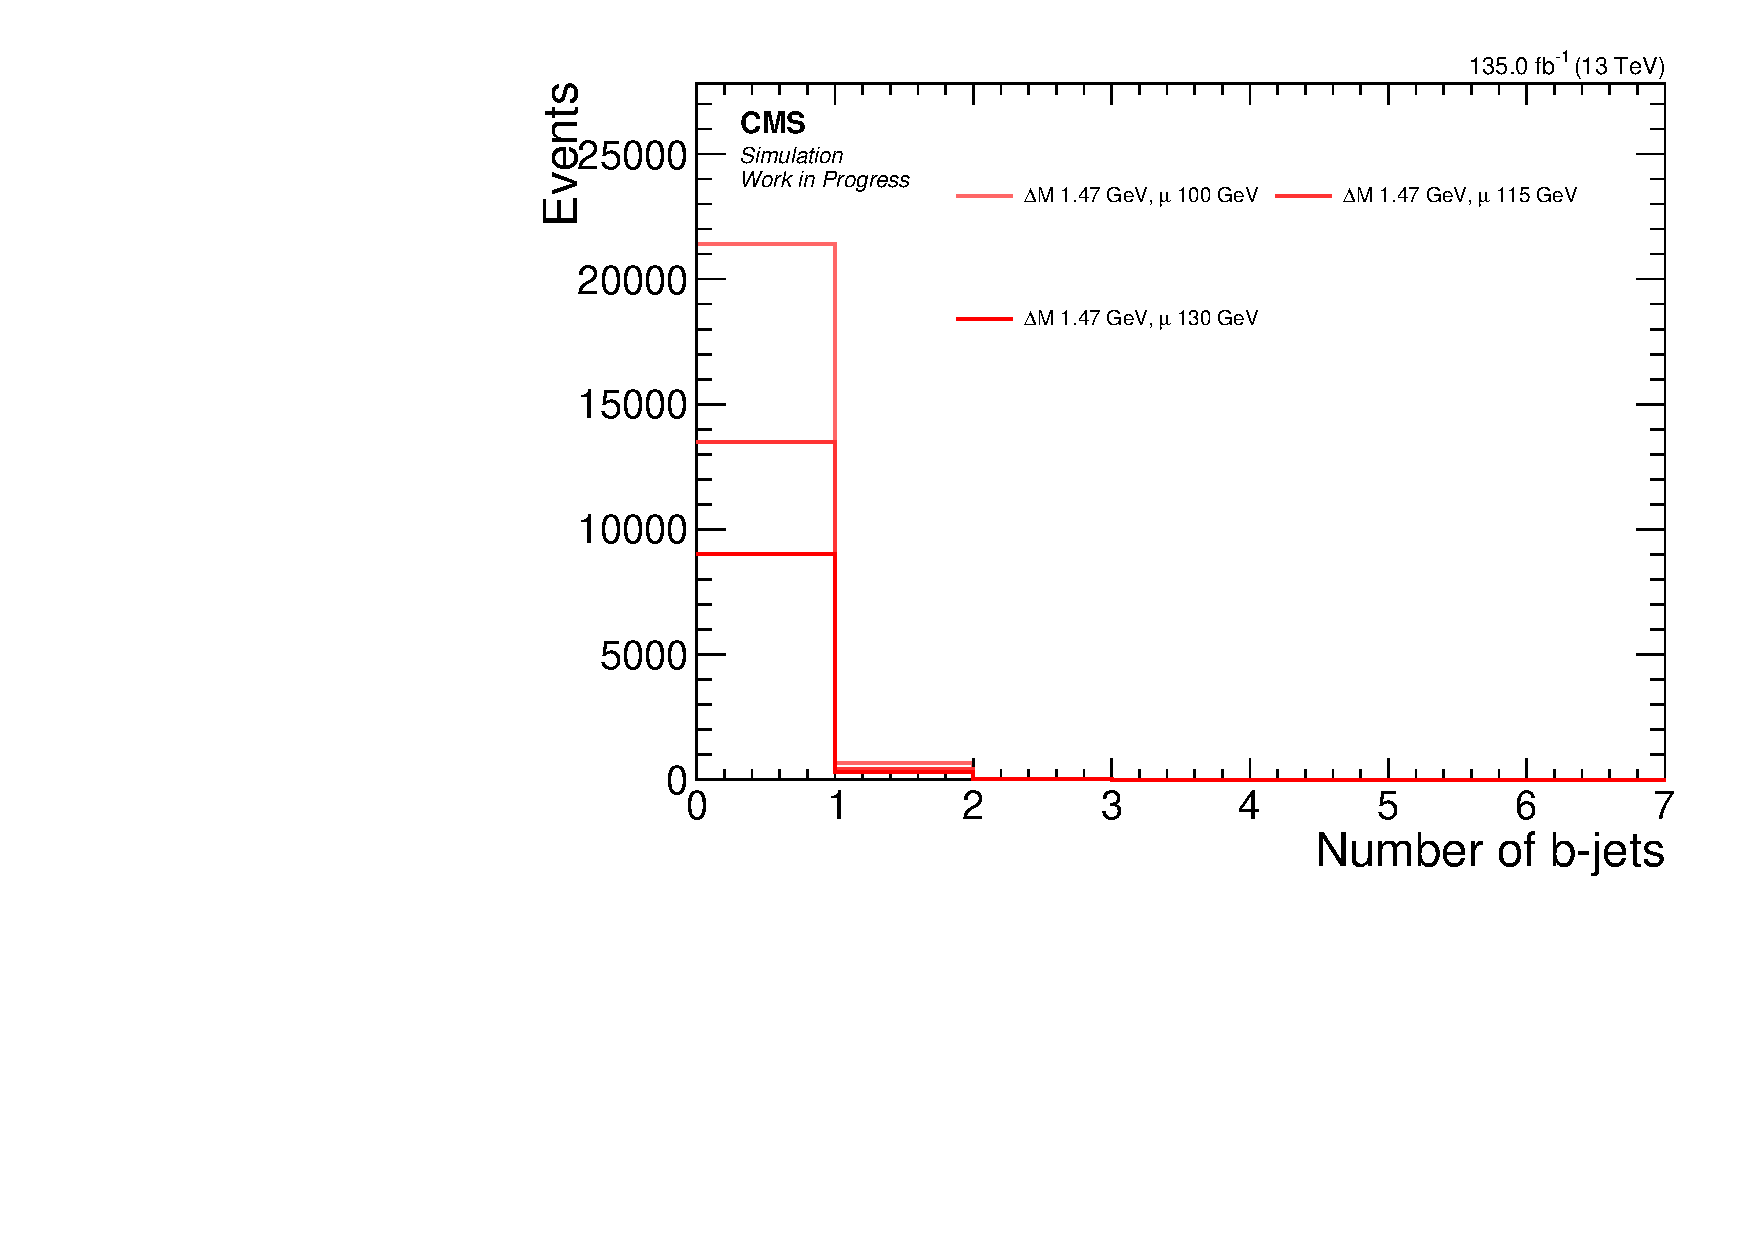
\includegraphics[width=0.48\linewidth]{plots/signal_common_distributions_fixed_dm/none_BTagsDeepMedium.pdf}  \\
\caption[Signal \emph{number of b-tagged jets} distributions]{ Signal distributions for \emph{number of b-tagged jets} comparing various $\dm$ with a fixed higgsino parameter $\mu=100\GeV$ (left), and comparing various higgsino parameters $\mu$ with fixed $\dm=1.47\GeV$ (right).}
\label{fig:signal-bjets}
\end{figure}

As an \gls{isr} jet is required in the event, it is expected that the \gls{met} and the \gls{mht} will be directed in the opposite direction of the jet, or at an angle close to $\pi$. This feature will not be observed in events with multiple jets in the \gls{sm} background, such as those arising from \gls{qcd}. To reduce the \gls{qcd} background, a requirement of $\mindphimhtjets > 0.4$ is imposed.

\begin{figure}[!htb]
\centering
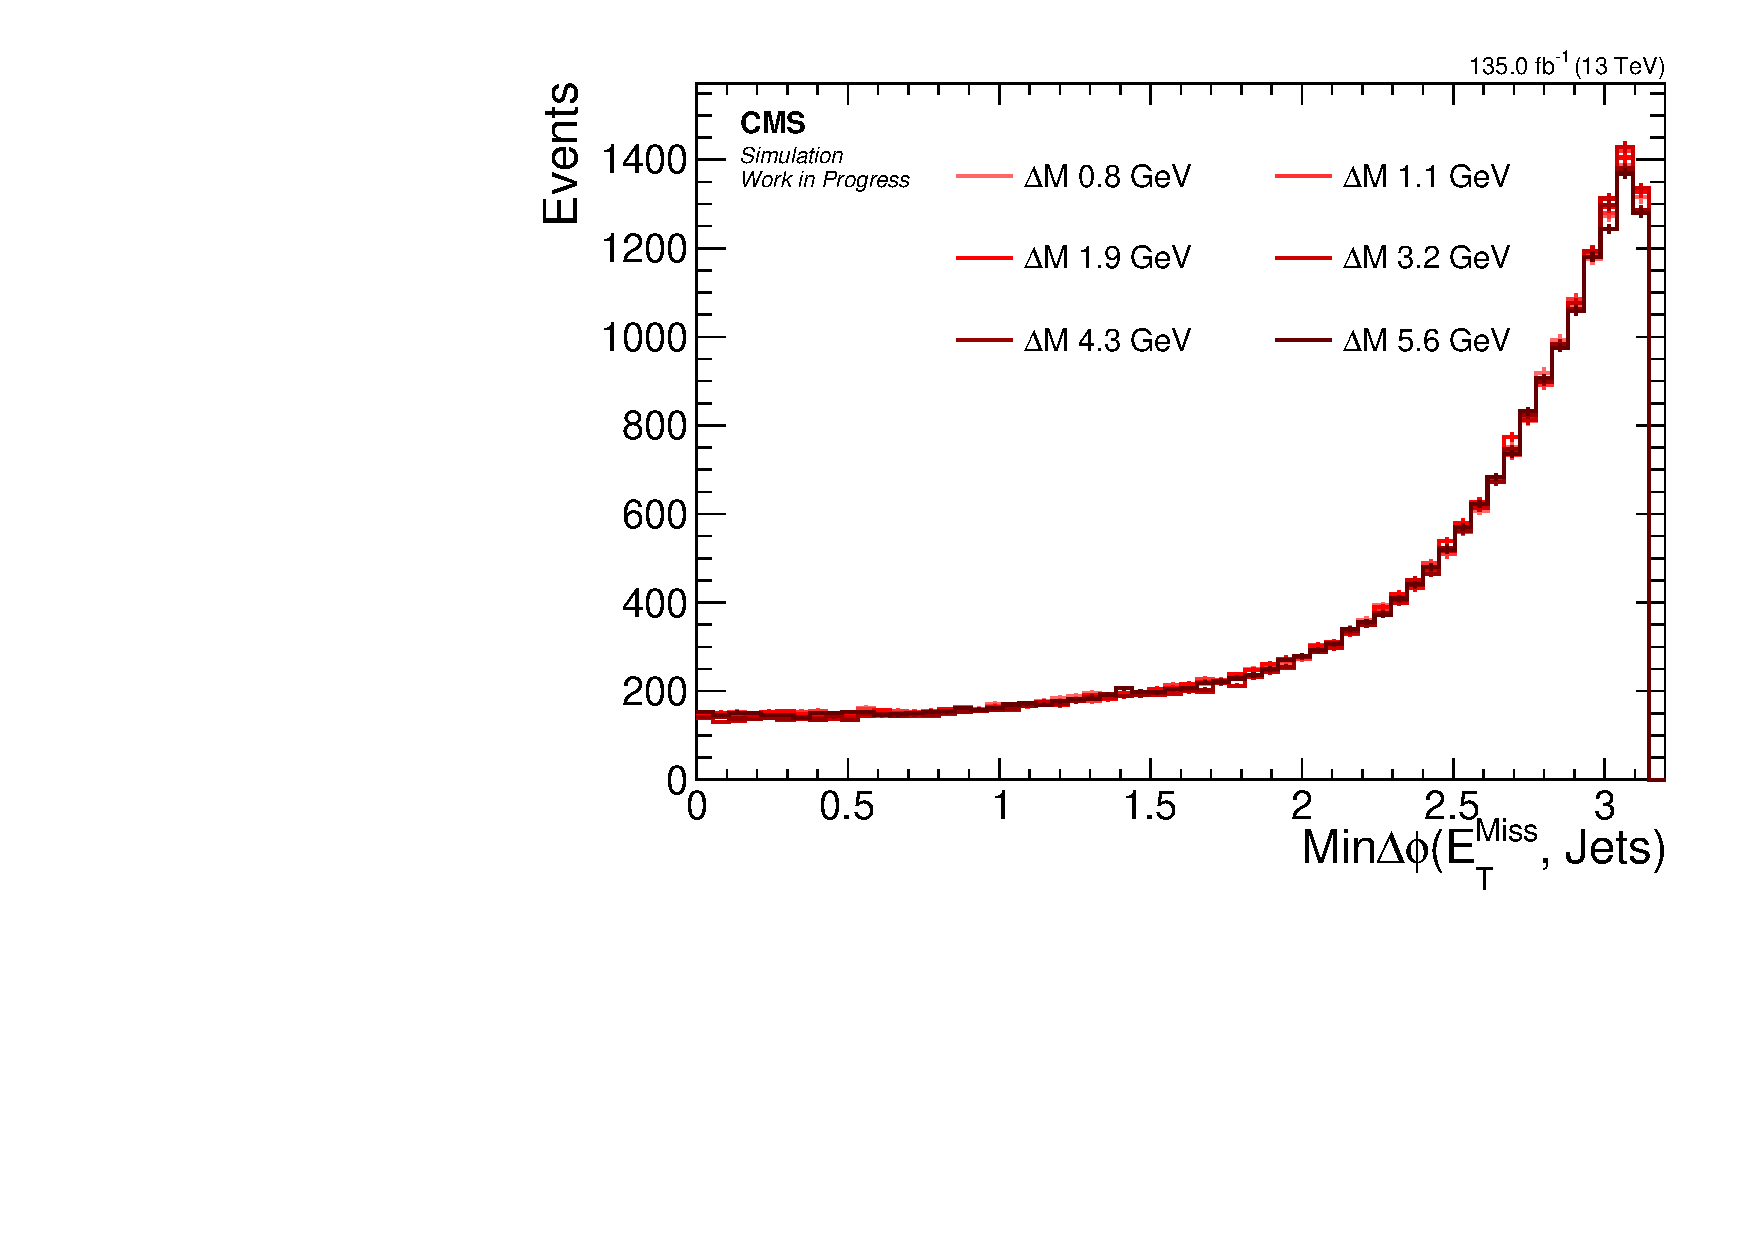
\includegraphics[width=0.48\linewidth]{plots/signal_common_distributions_fixed_mu/none_MinDeltaPhiMetJets.pdf} \,
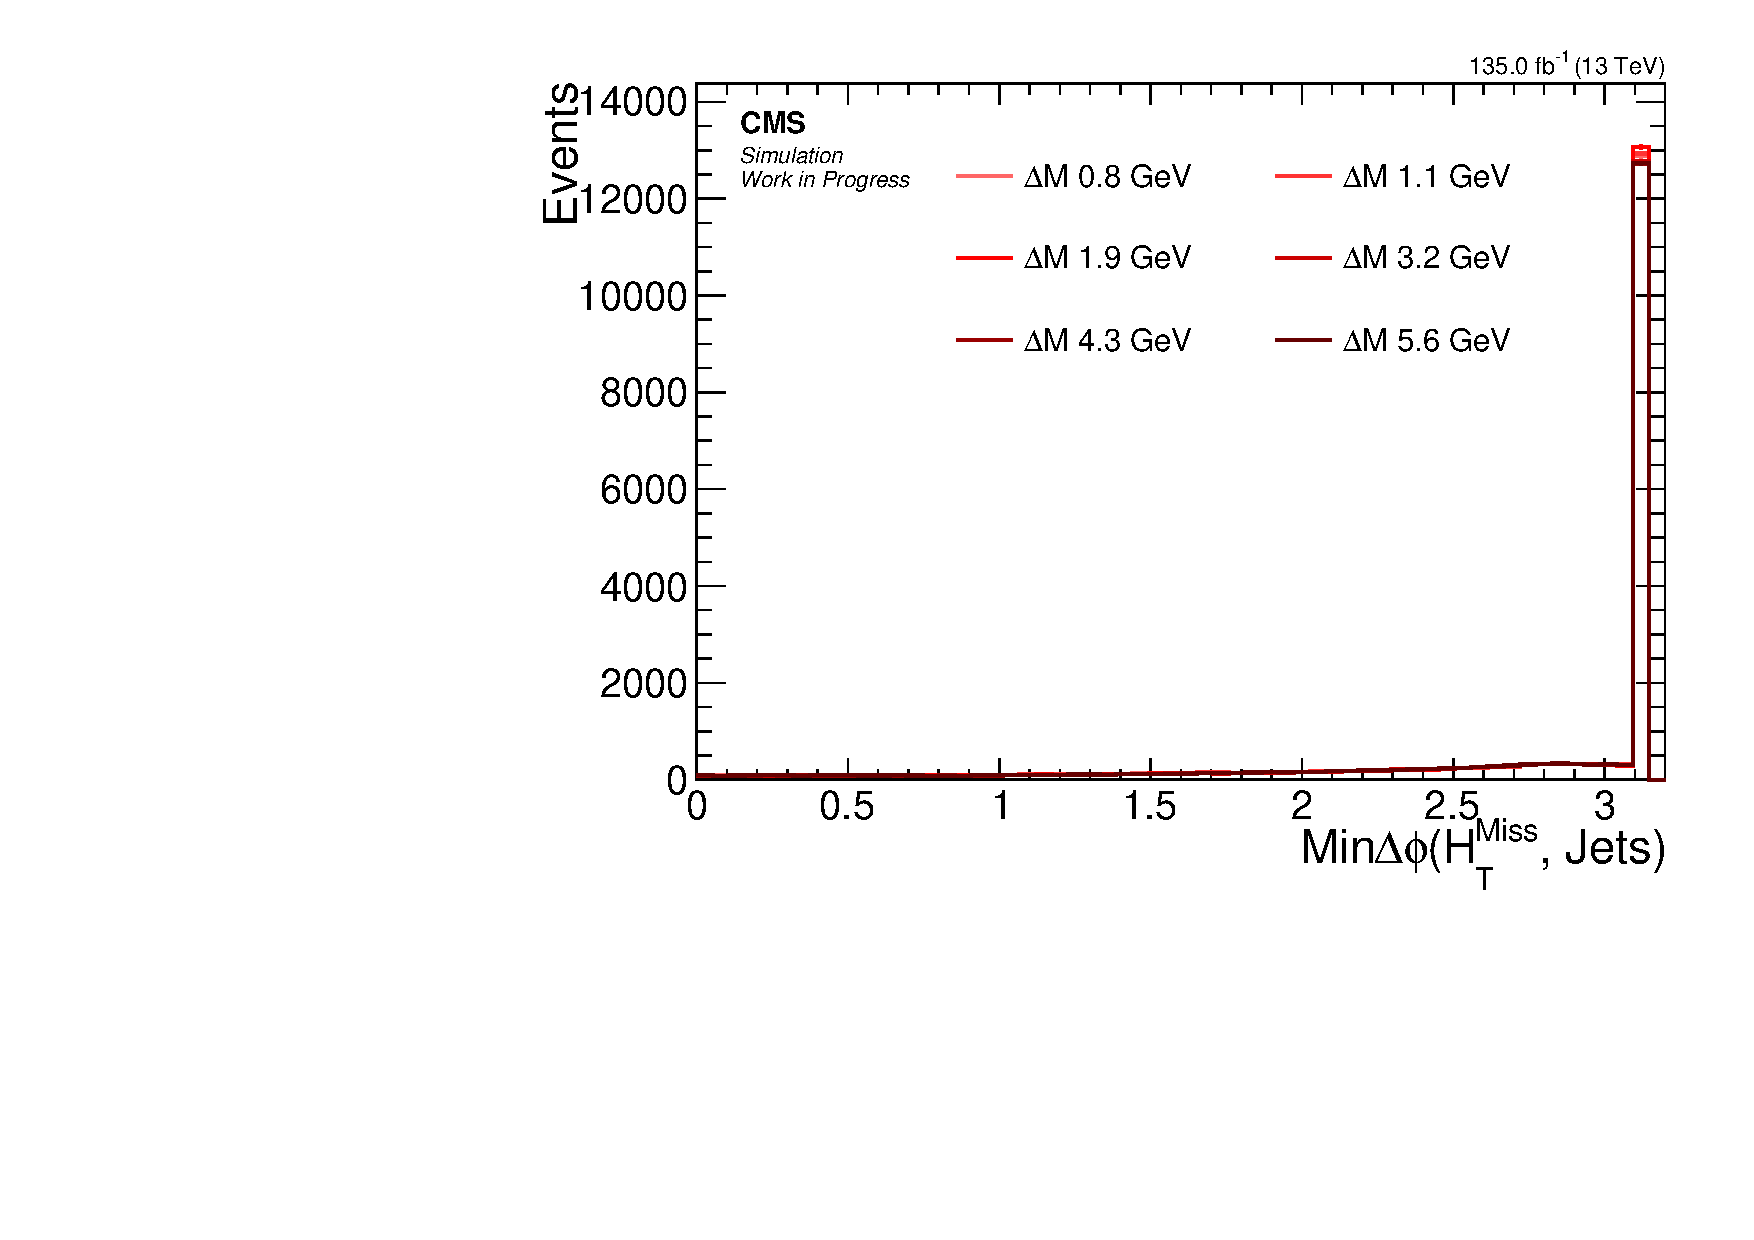
\includegraphics[width=0.48\linewidth]{plots/signal_common_distributions_fixed_mu/none_MinDeltaPhiMhtJets.pdf}  \\
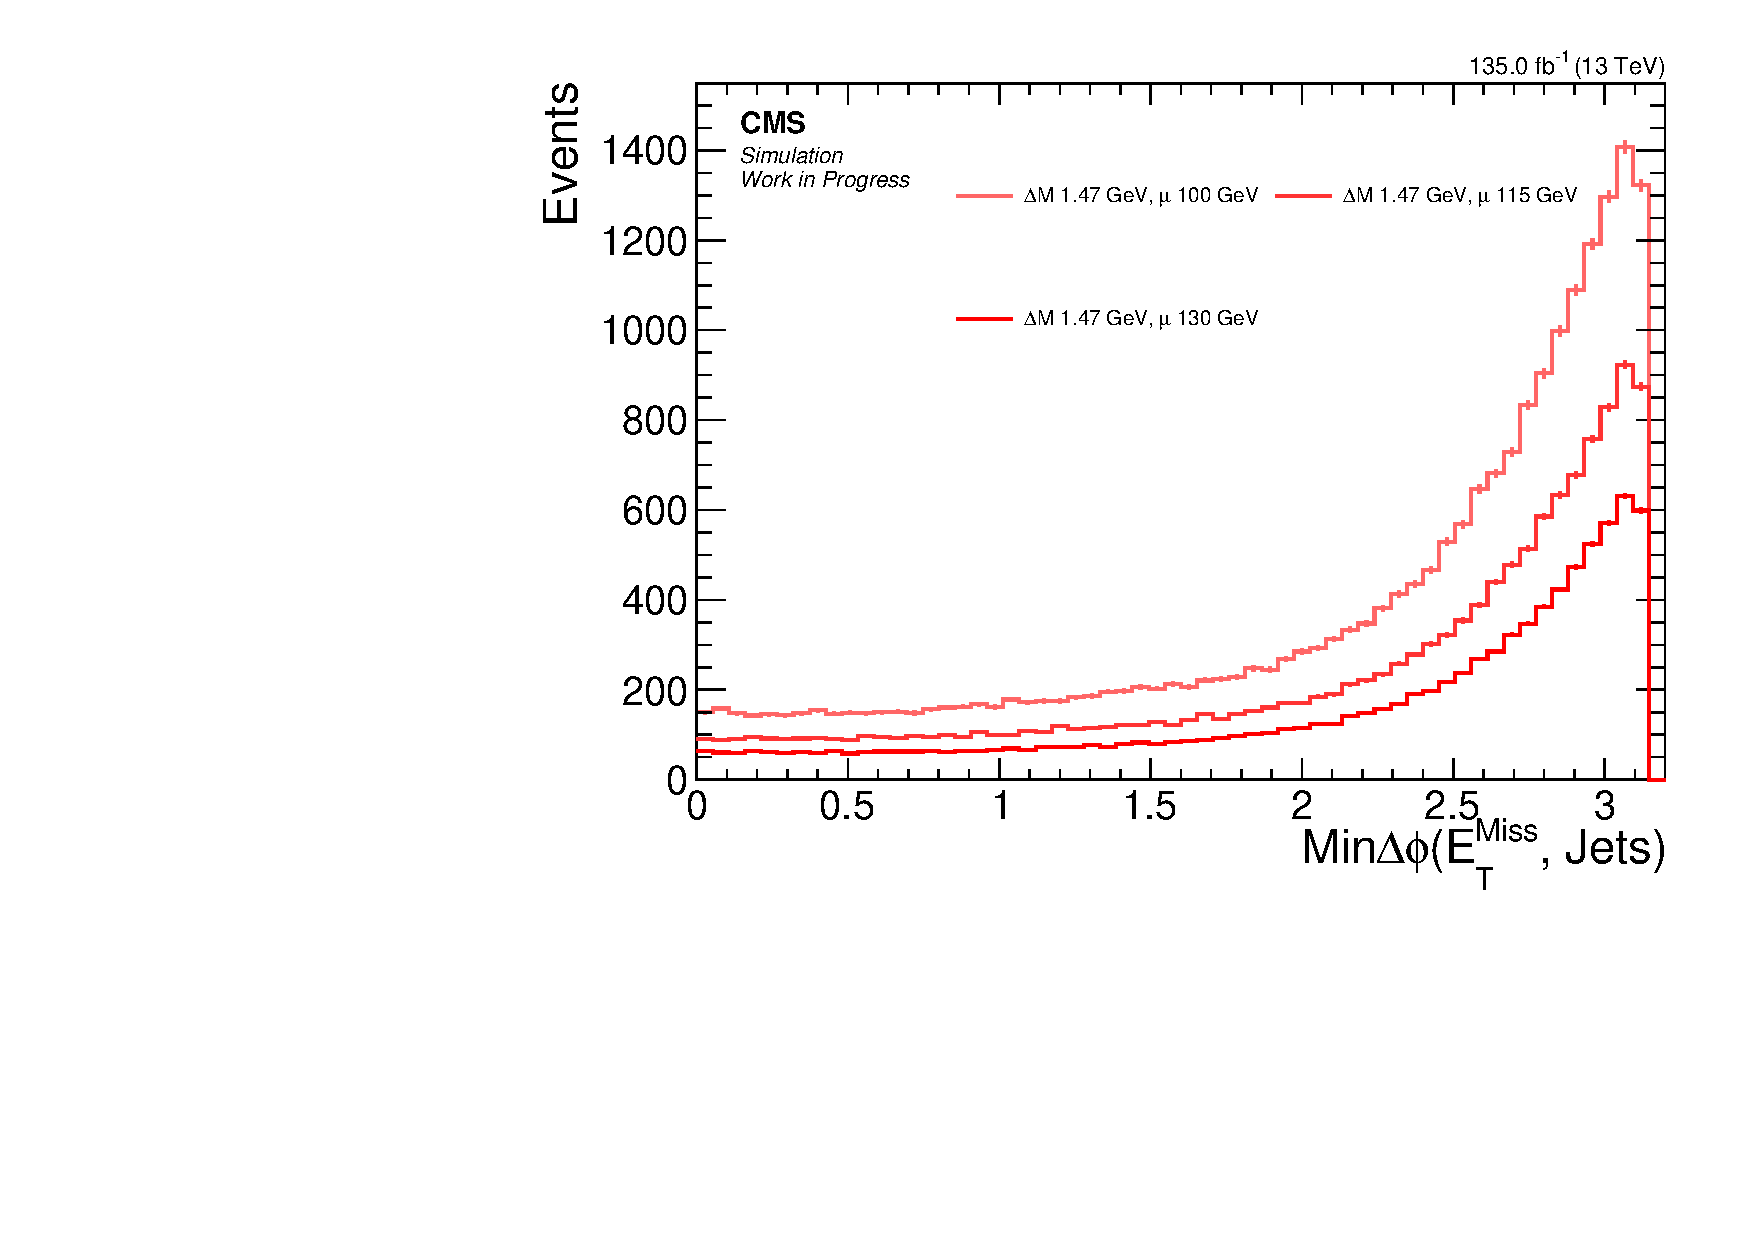
\includegraphics[width=0.48\linewidth]{plots/signal_common_distributions_fixed_dm/none_MinDeltaPhiMetJets.pdf} \,
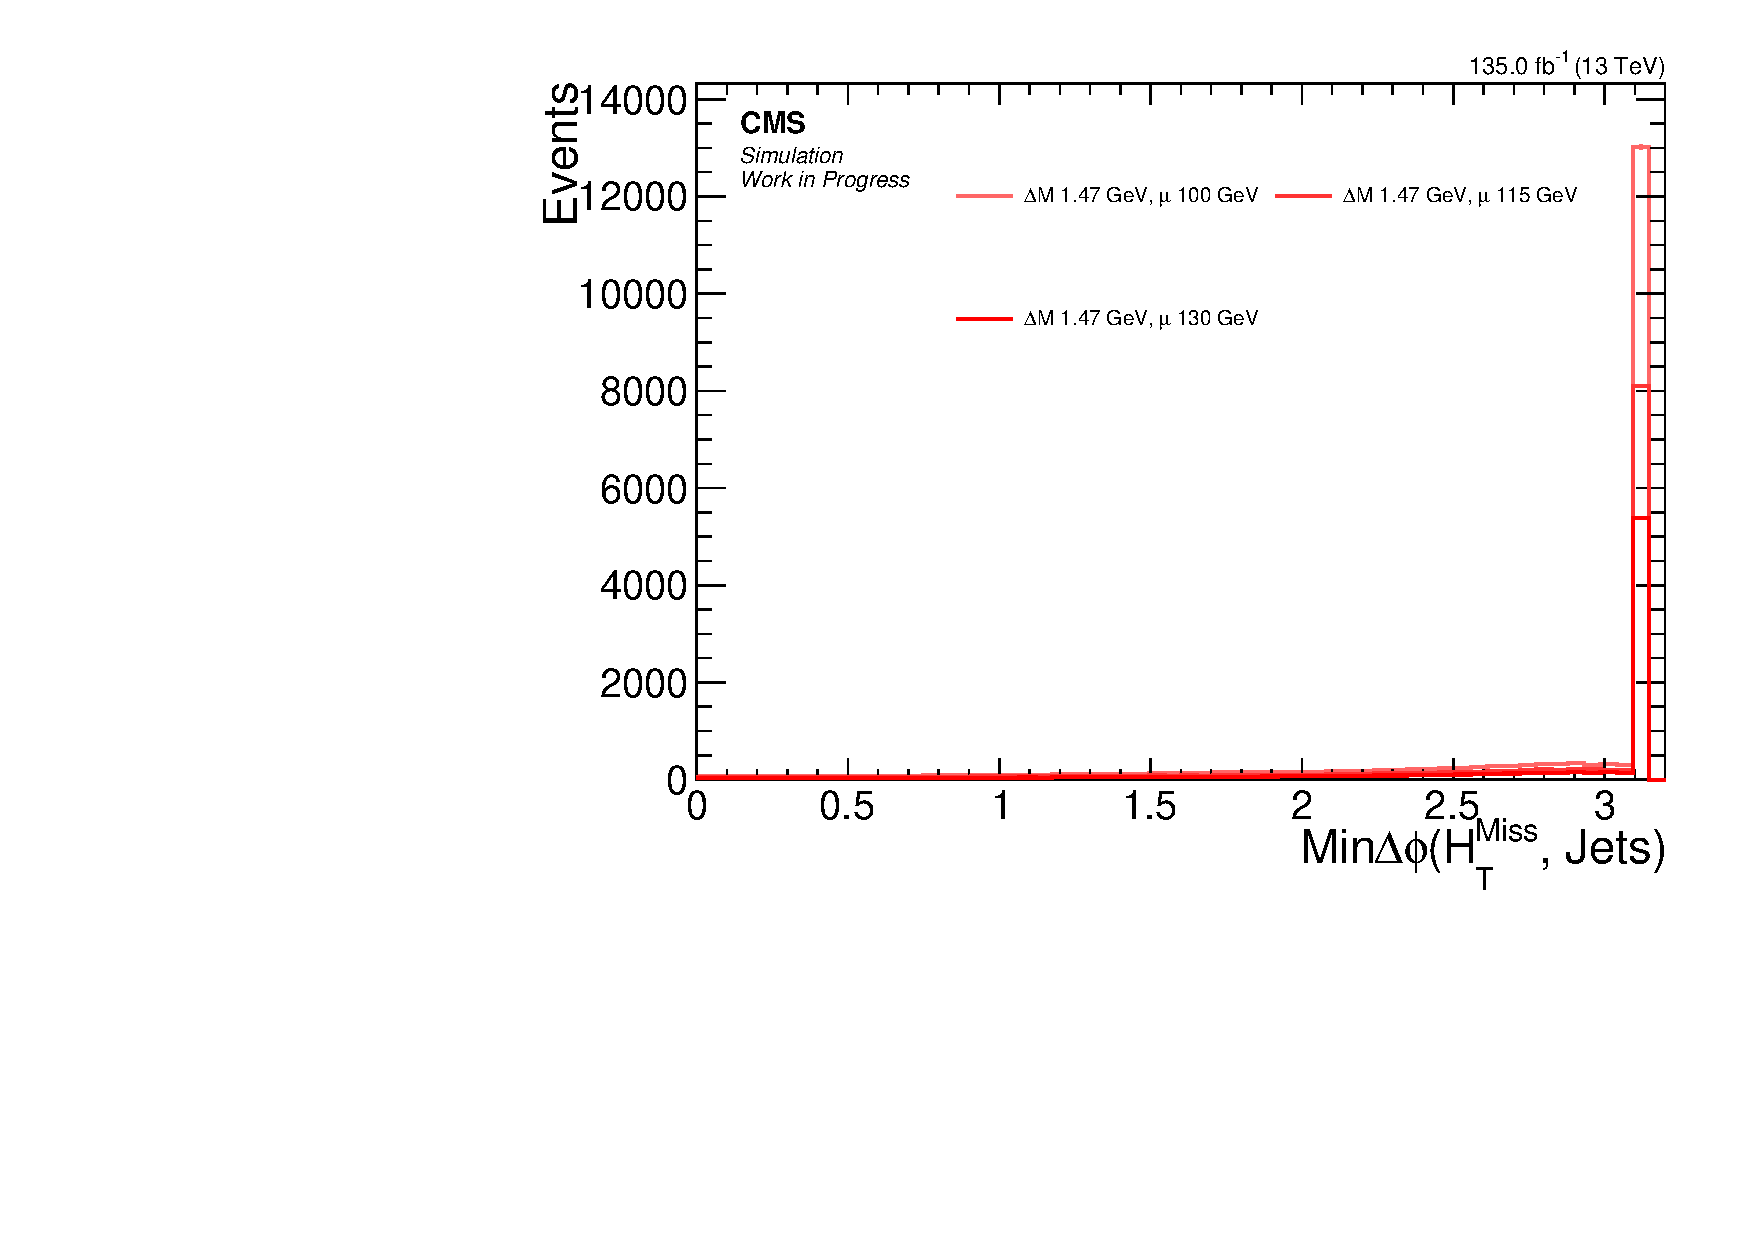
\includegraphics[width=0.48\linewidth]{plots/signal_common_distributions_fixed_dm/none_MinDeltaPhiMhtJets.pdf}  \\
\caption[Signal $\mindphimetjets$ and $\mindphimhtjets$ distributions]{ Signal distributions for \mindphimetjets (left) and \mindphimhtjets (right) comparing various $\dm$ with a fixed higgsino parameter $\mu=100\GeV$ (upper), and comparing various higgsino parameters $\mu$ with fixed $\dm=1.47\GeV$ (lower).}
\label{fig:signal-min-deltaphi-met-mht}
\end{figure}

\subsection{Base selection}

The section is recapped by summarizing the base selection of the analysis. The base selection, also known interchangeably as the preselection, is applied to all analysis categories. It ls listed in Table~\ref{tab:base-selection}.

\begin{table}[!htb]
	\centering
	\label{tab:base-selection}
		\caption{Base selection applied to all analysis categories}
		%\vspace{1mm}
			\begin{tabular}{lc} \hline
			Variable & Value \\ \hline
			$\mht \left[\GeV\right]$ & $\geq220$ \\
			$\njets \left( \pt \geq 30\GeV\, \mathrm{and}\, \abs{\eta} < 2.4 \right)$ & $\geq 1$\\
			$\nbjets \left( \pt \geq 30\GeV\, \mathrm{and}\, \abs{\eta} < 2.4 \right)$ & 0 \\
			$\mindphimhtjets$ & $ > 0.4$ \\ \hline
			\end{tabular}
\end{table}

\clearpage
\subsection{Dilepton kinematics}

Kinematic distributions have been examined so far, with the leptons in the event ignored. However, the dilepton system contains the most distinctive features of the signal. To fully understand the unique phase space of the dilepton system, generator level distributions are examined first, followed by an exploration of the effects of reconstruction on those observables. Since the dimuon category is the most sensitive due to its lower threshold on the leptons' transverse momentum, events with two electrons are excluded from the following sections, focusing on the muons. The kinematics change dramatically as a function of \dm. In contrast, the higgsino parameter $\mu$ effects almost only the overall normalization due to the different production cross section. Therefore, the higgsino parameter is set to $\mu=100\GeV$ in the following sections, with the \dm varied.

\subsubsection{Lepton $\eta$ and transverse momentum \gls{pt}}
\label{sec:muon-eta-pt}

The signal acceptance and sensitivity are significantly impacted by the accessible thresholds of the transverse momentum \gls{pt} distribution of the muons. The muon reconstruction process and details are discussed in Section~\ref{id-muons}. The selection applied to the muons in this analysis is described in Section~\ref{sec:muon-selection} and referred to as \emph{analysis selection}. This section aims to examine the importance of the \gls{pt} on the signal and its dilepton kinematic distributions.

The generator level distribution of \gls{pt}, or the so-called \emph{truth} distributions, which do not exhibit any detector or reconstruction features, are examined first. The reconstructed distribution is then compared with the generator level distribution in Figure~\ref{fig:signal-muons-pt}. 

\begin{figure}[!htb]
\centering
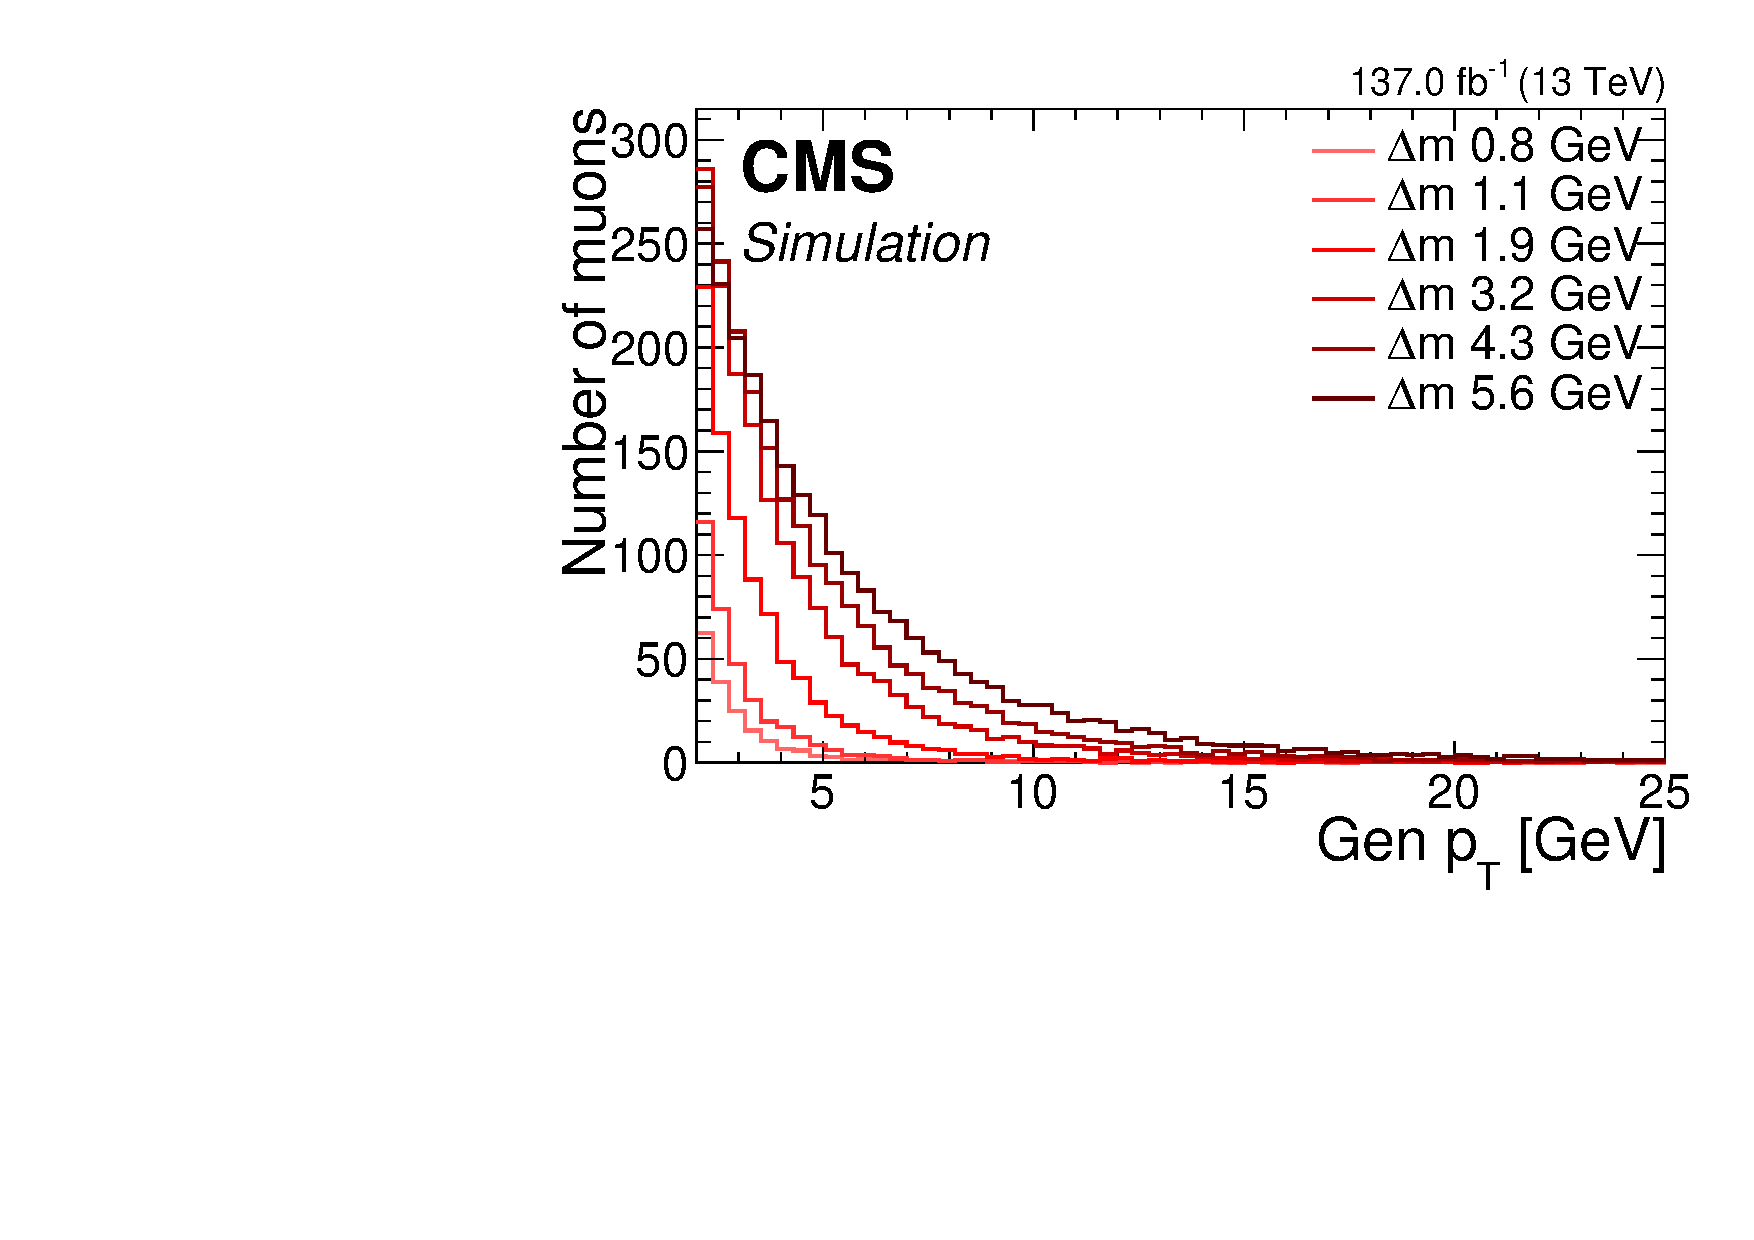
\includegraphics[width=0.32\linewidth]{plots/signal_muons_gen/none_Muons_pt.pdf} \,
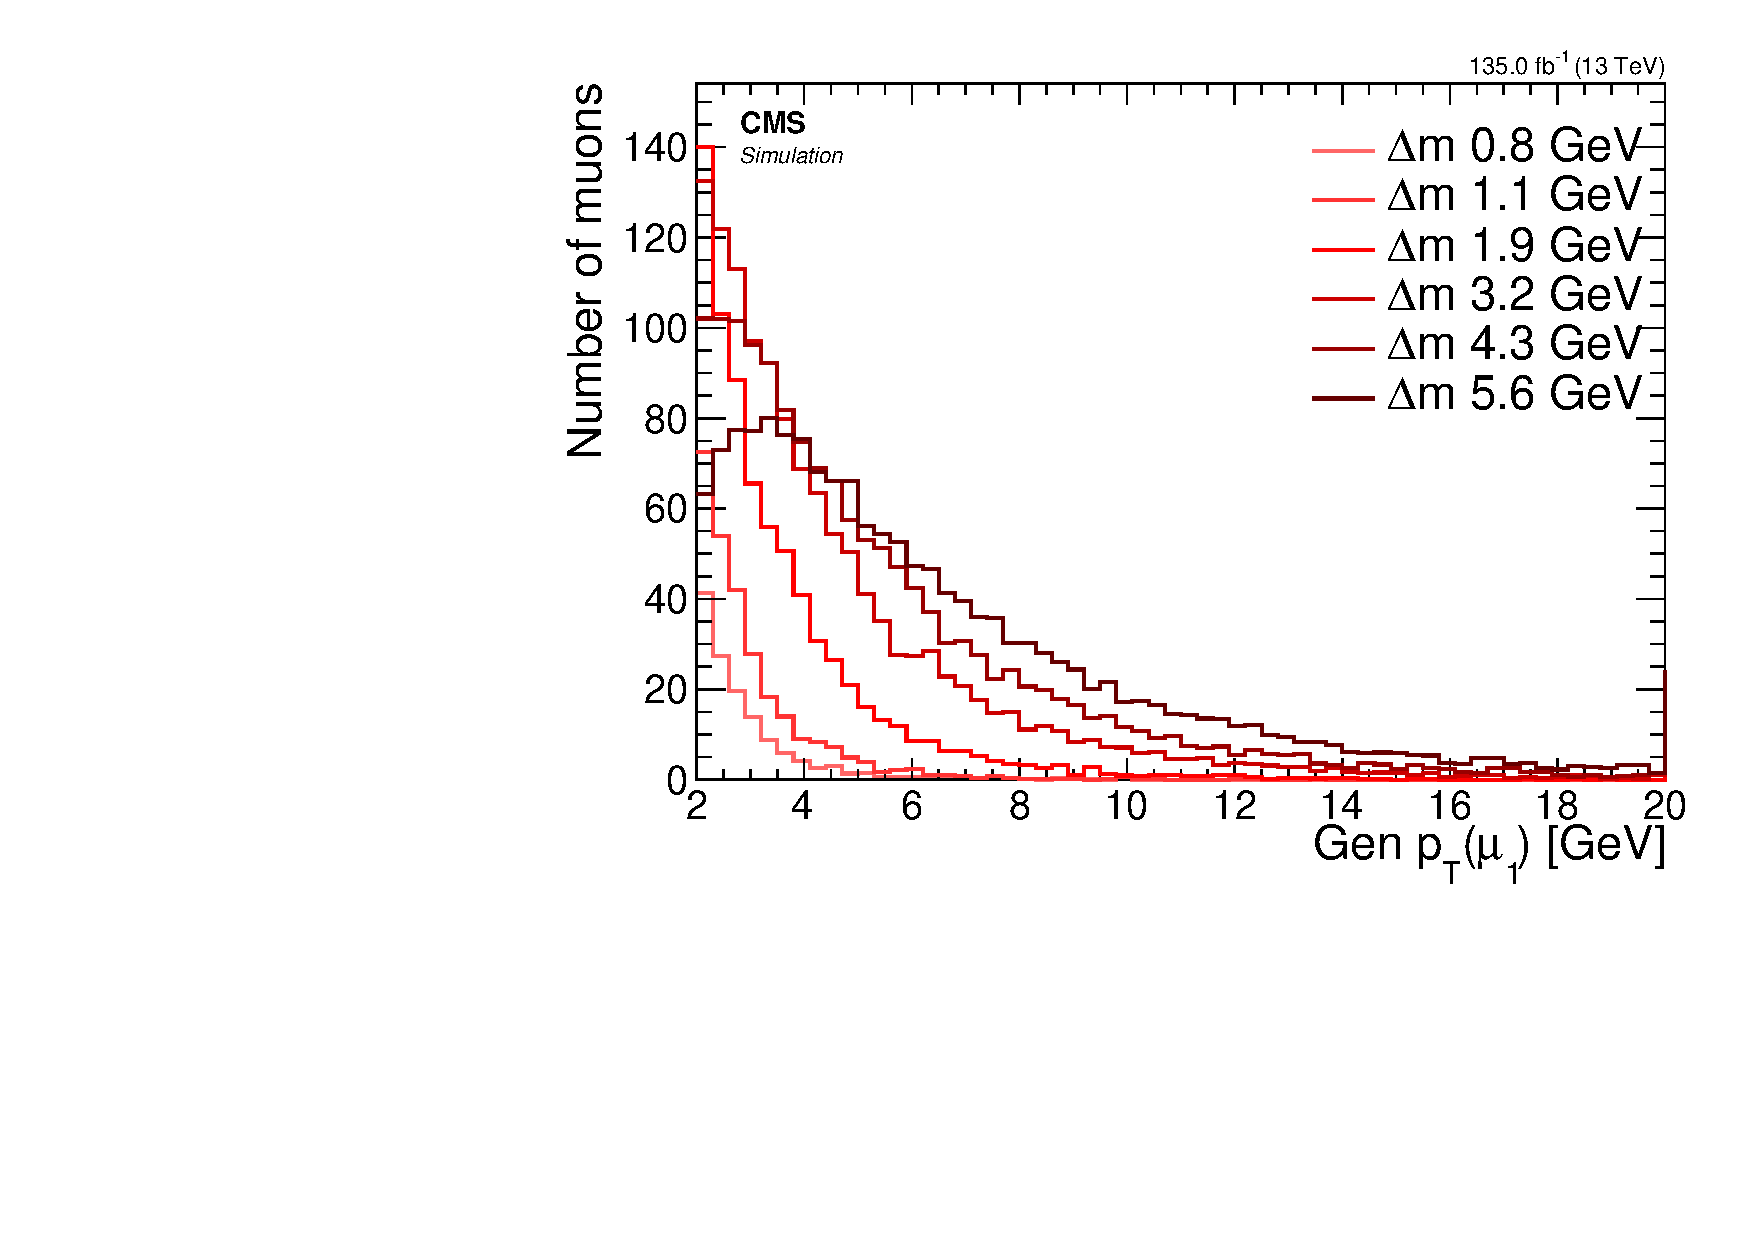
\includegraphics[width=0.32\linewidth]{plots/signal_muons_gen/none_Muons_m1_pt.pdf}  \,
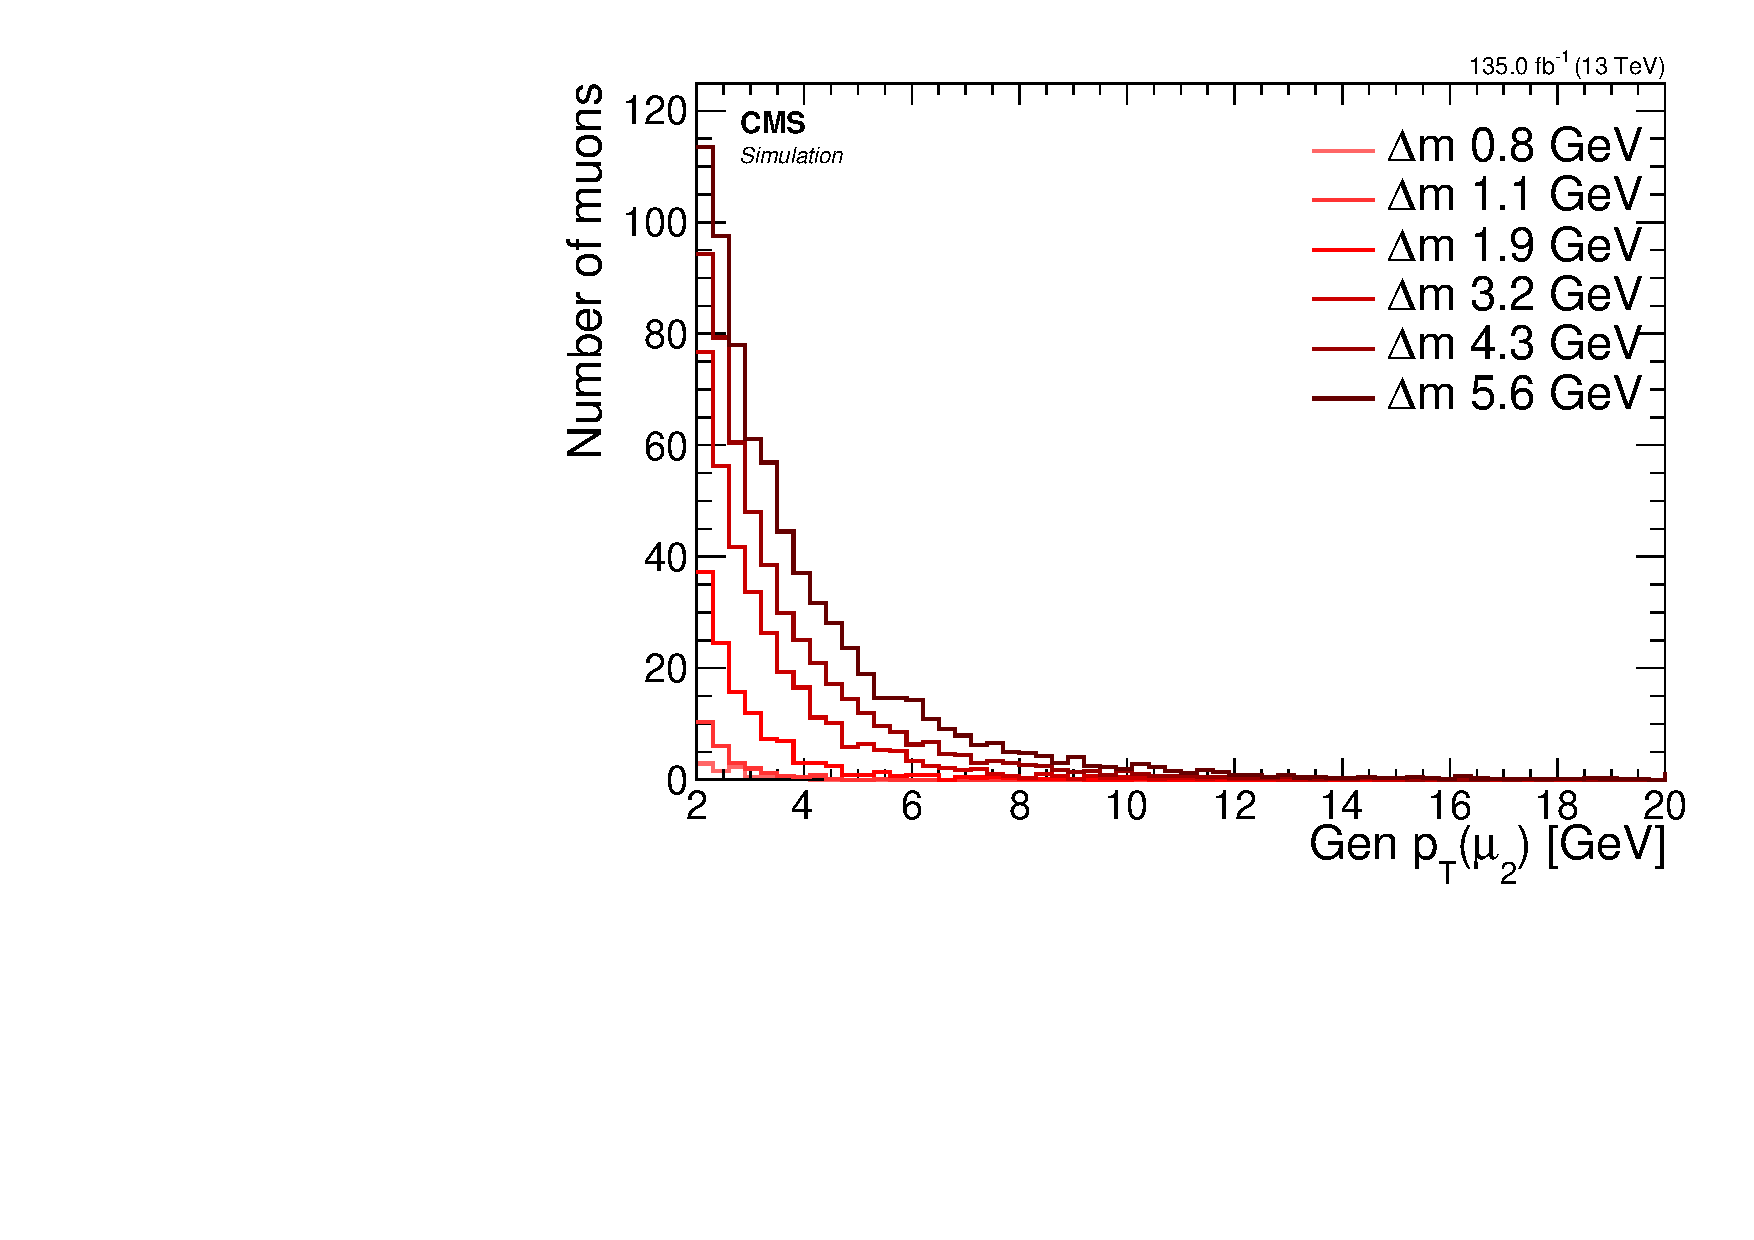
\includegraphics[width=0.32\linewidth]{plots/signal_muons_gen/none_Muons_m2_pt.pdf} \\
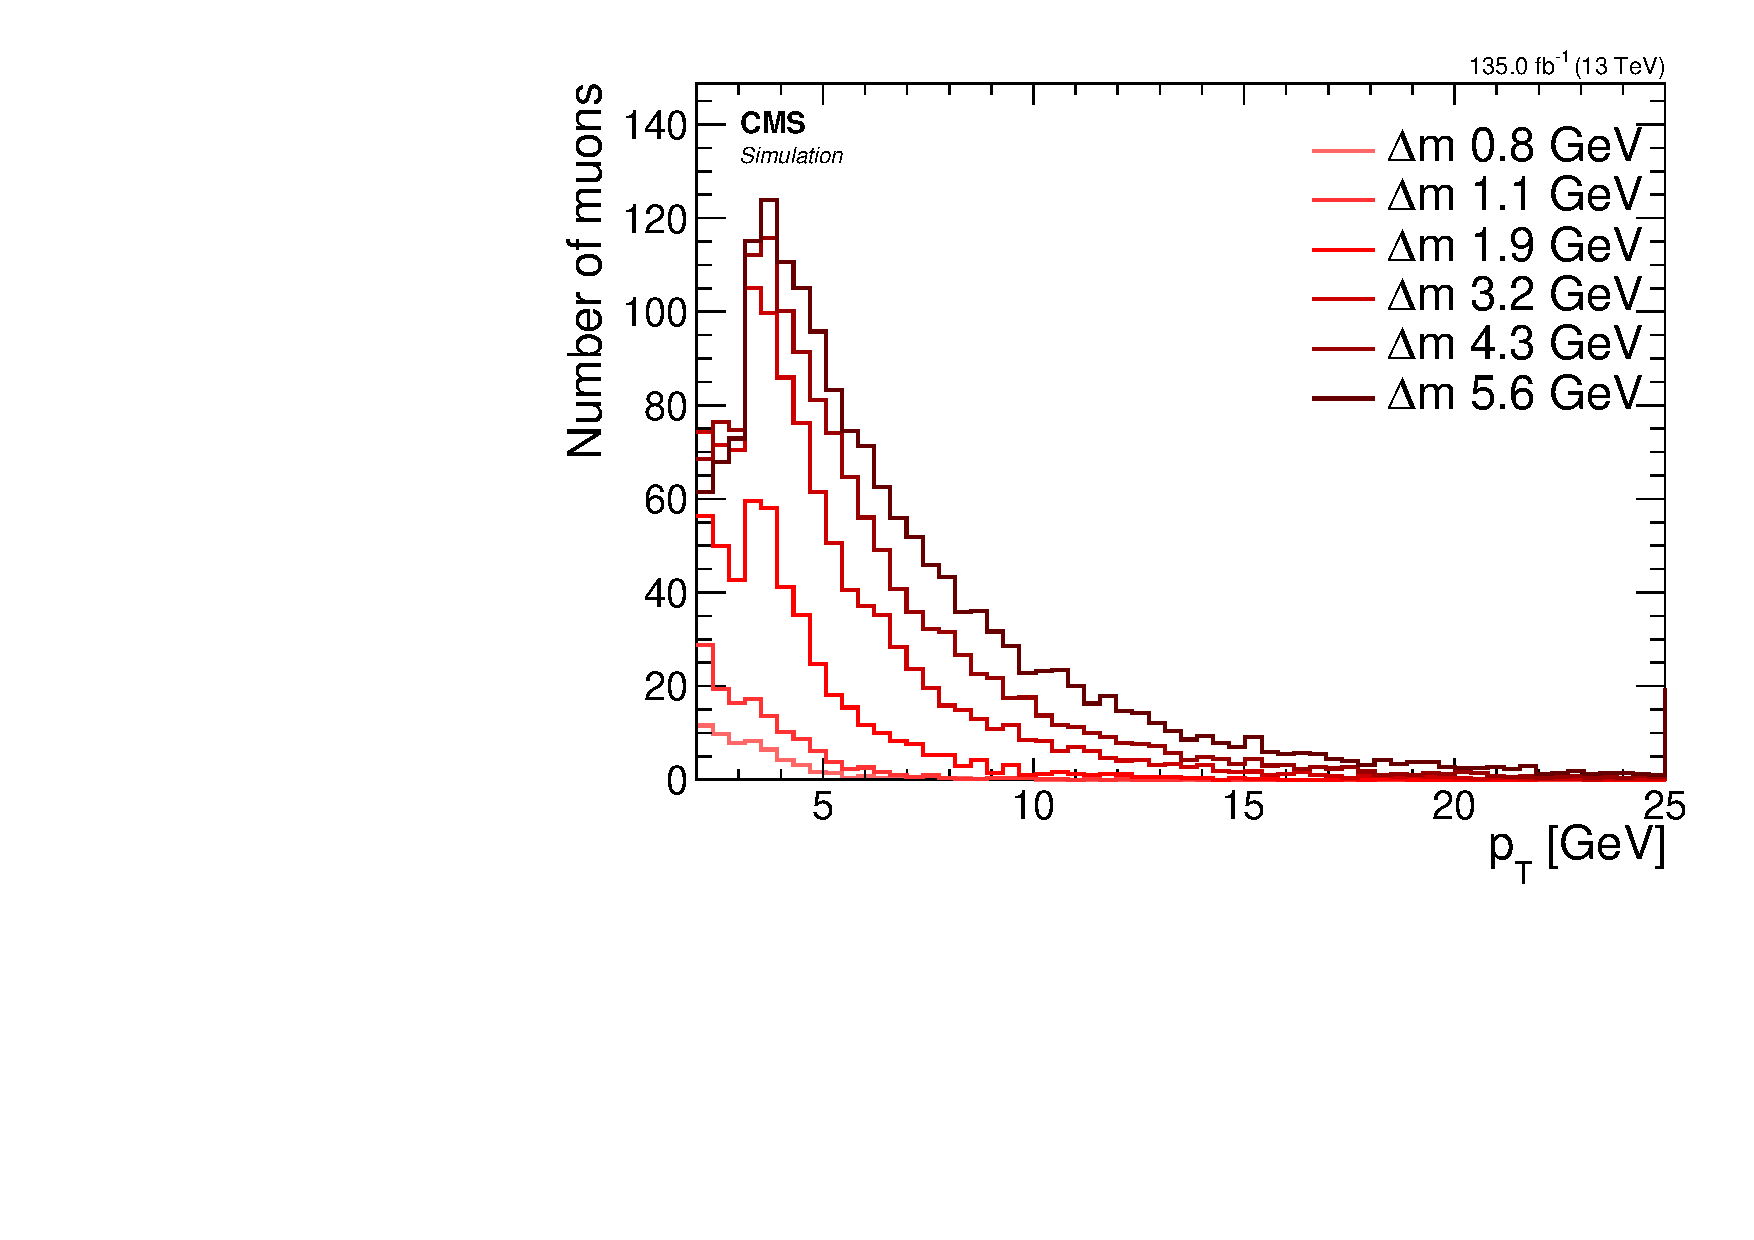
\includegraphics[width=0.32\linewidth]{plots/signal_muons/none_Muons_pt.pdf} \,
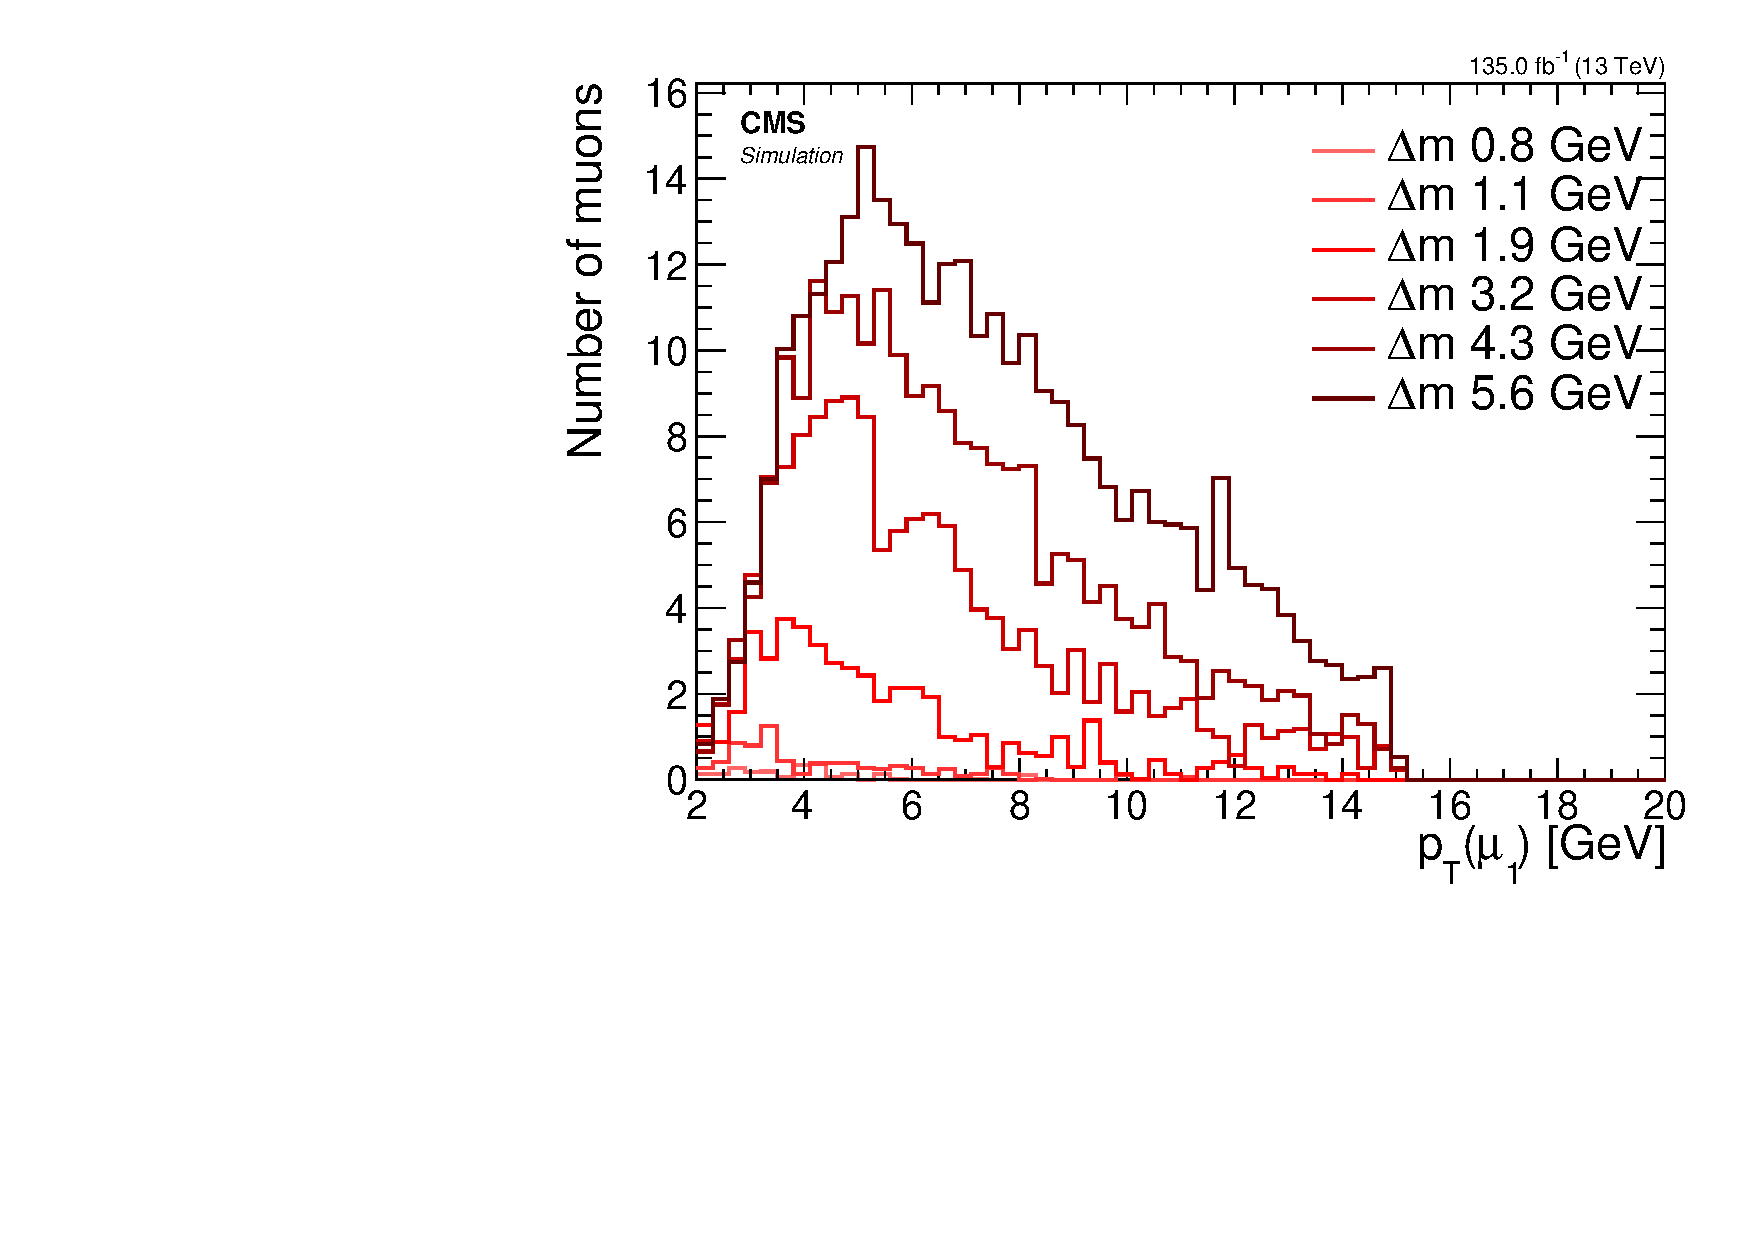
\includegraphics[width=0.32\linewidth]{plots/signal_muons/none_Muons_m1_pt.pdf}  \,
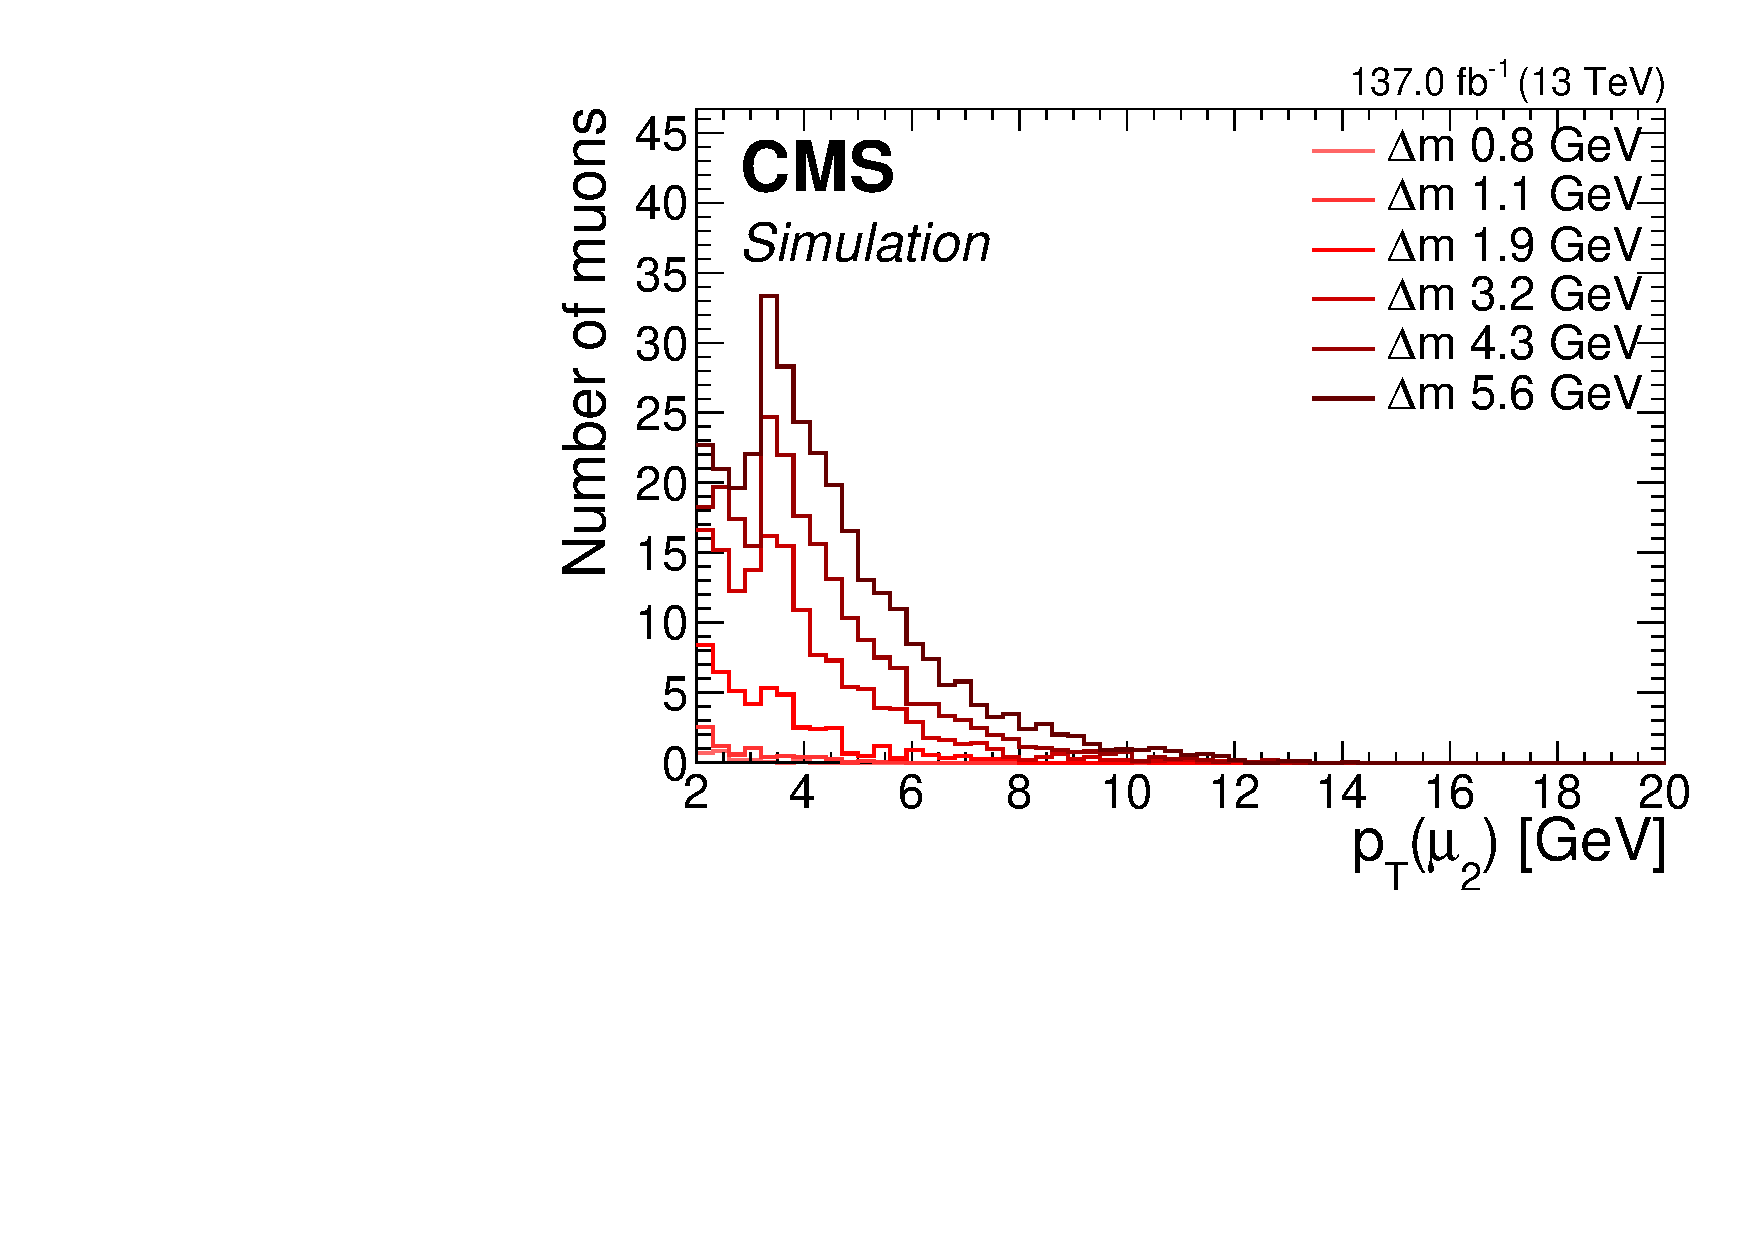
\includegraphics[width=0.32\linewidth]{plots/signal_muons/none_Muons_m2_pt.pdf} \\
\caption[Signal \pt distributions]{ Signal \pt distributions for inclusive (left), leading muon $\mu_1$ (middle),  subleading muon $\mu_2$ (right) at generator level (top) and reconstruction level passing analysis selection (bottom). }
\label{fig:signal-muons-pt}
\end{figure}

When comparing the generator level to the reconstruction level of the inclusive \pt distribution, it becomes apparent that a reshaping occurs around $3 \GeV$. A significant proportion of the generated muons with $\pt<3\GeV$ is lost in the reconstruction process. The subleading muon \pt distribution at the reconstruction level has a camel shape, whereby the efficiency drops below a \pt of $3\GeV$ and is only partially regained at $\pt<3\GeV$. This effect is due to the detector and is more clearly visible when splitting the \pt distribution into a barrel ($\abs{\eta} < 1.2$) and encaps ($\abs{\eta} \geq 1.2$) portions, as shown in Figure~\ref{fig:signal-pt-barrel-endcaps}.

\begin{figure}[!htb]
\centering
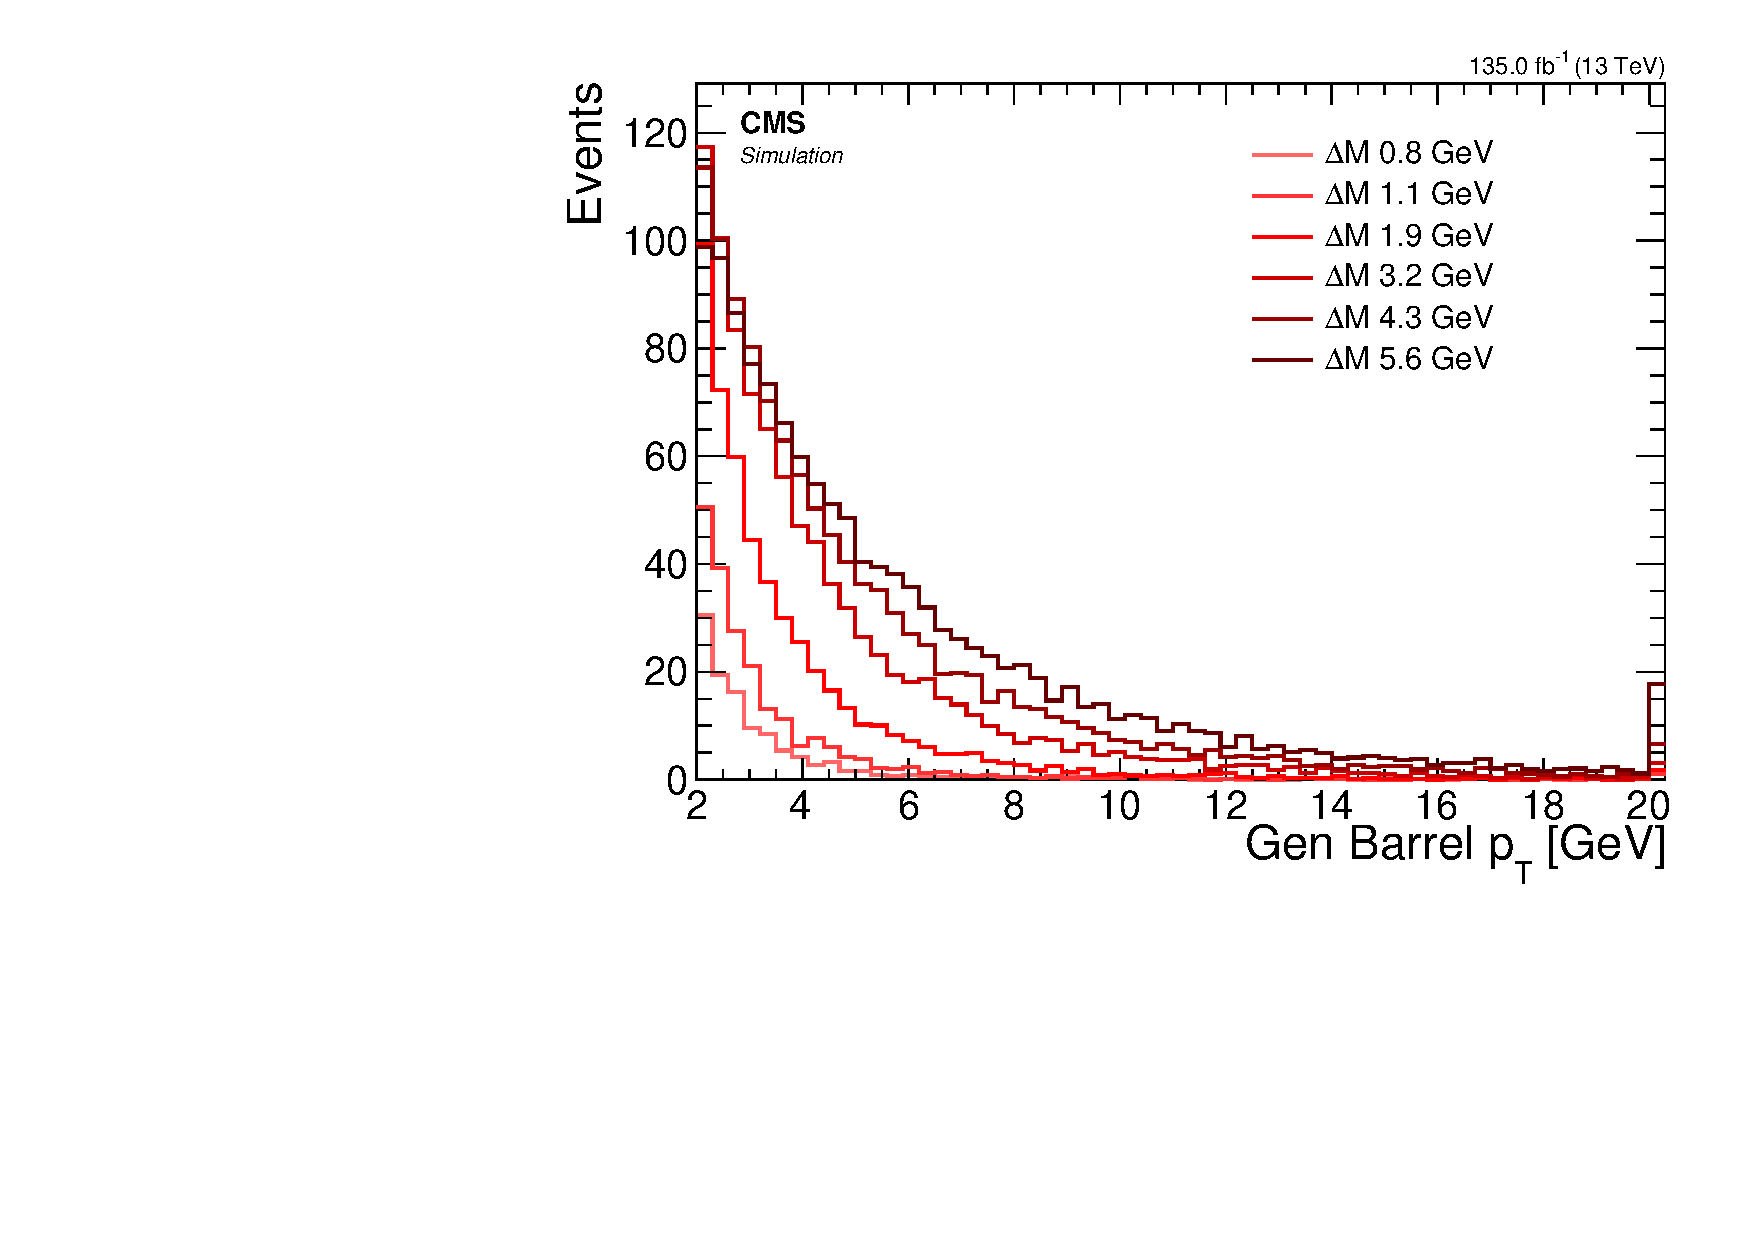
\includegraphics[width=0.48\linewidth]{plots/signal_muons_gen/none_Muons_pt_barrel.pdf} \,
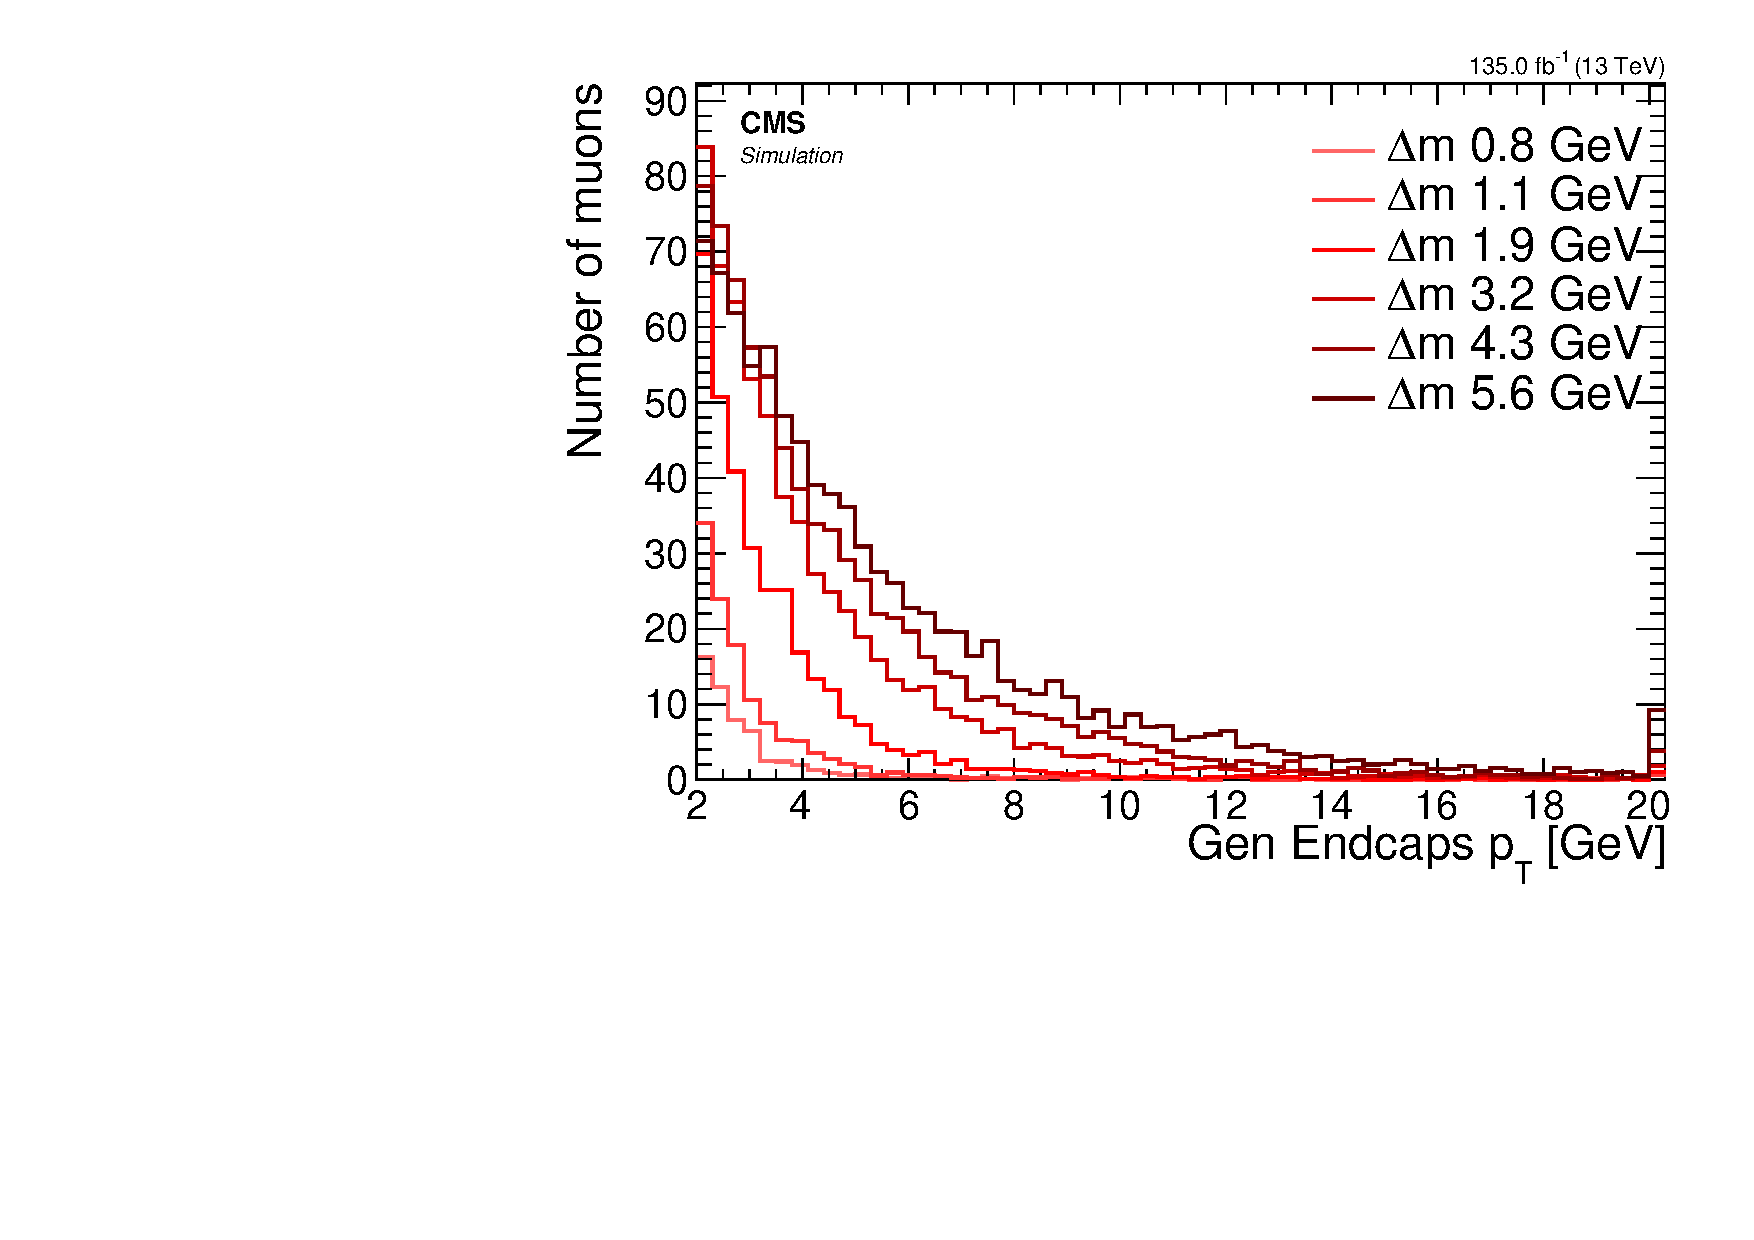
\includegraphics[width=0.48\linewidth]{plots/signal_muons_gen/none_Muons_pt_endcape.pdf}  \\
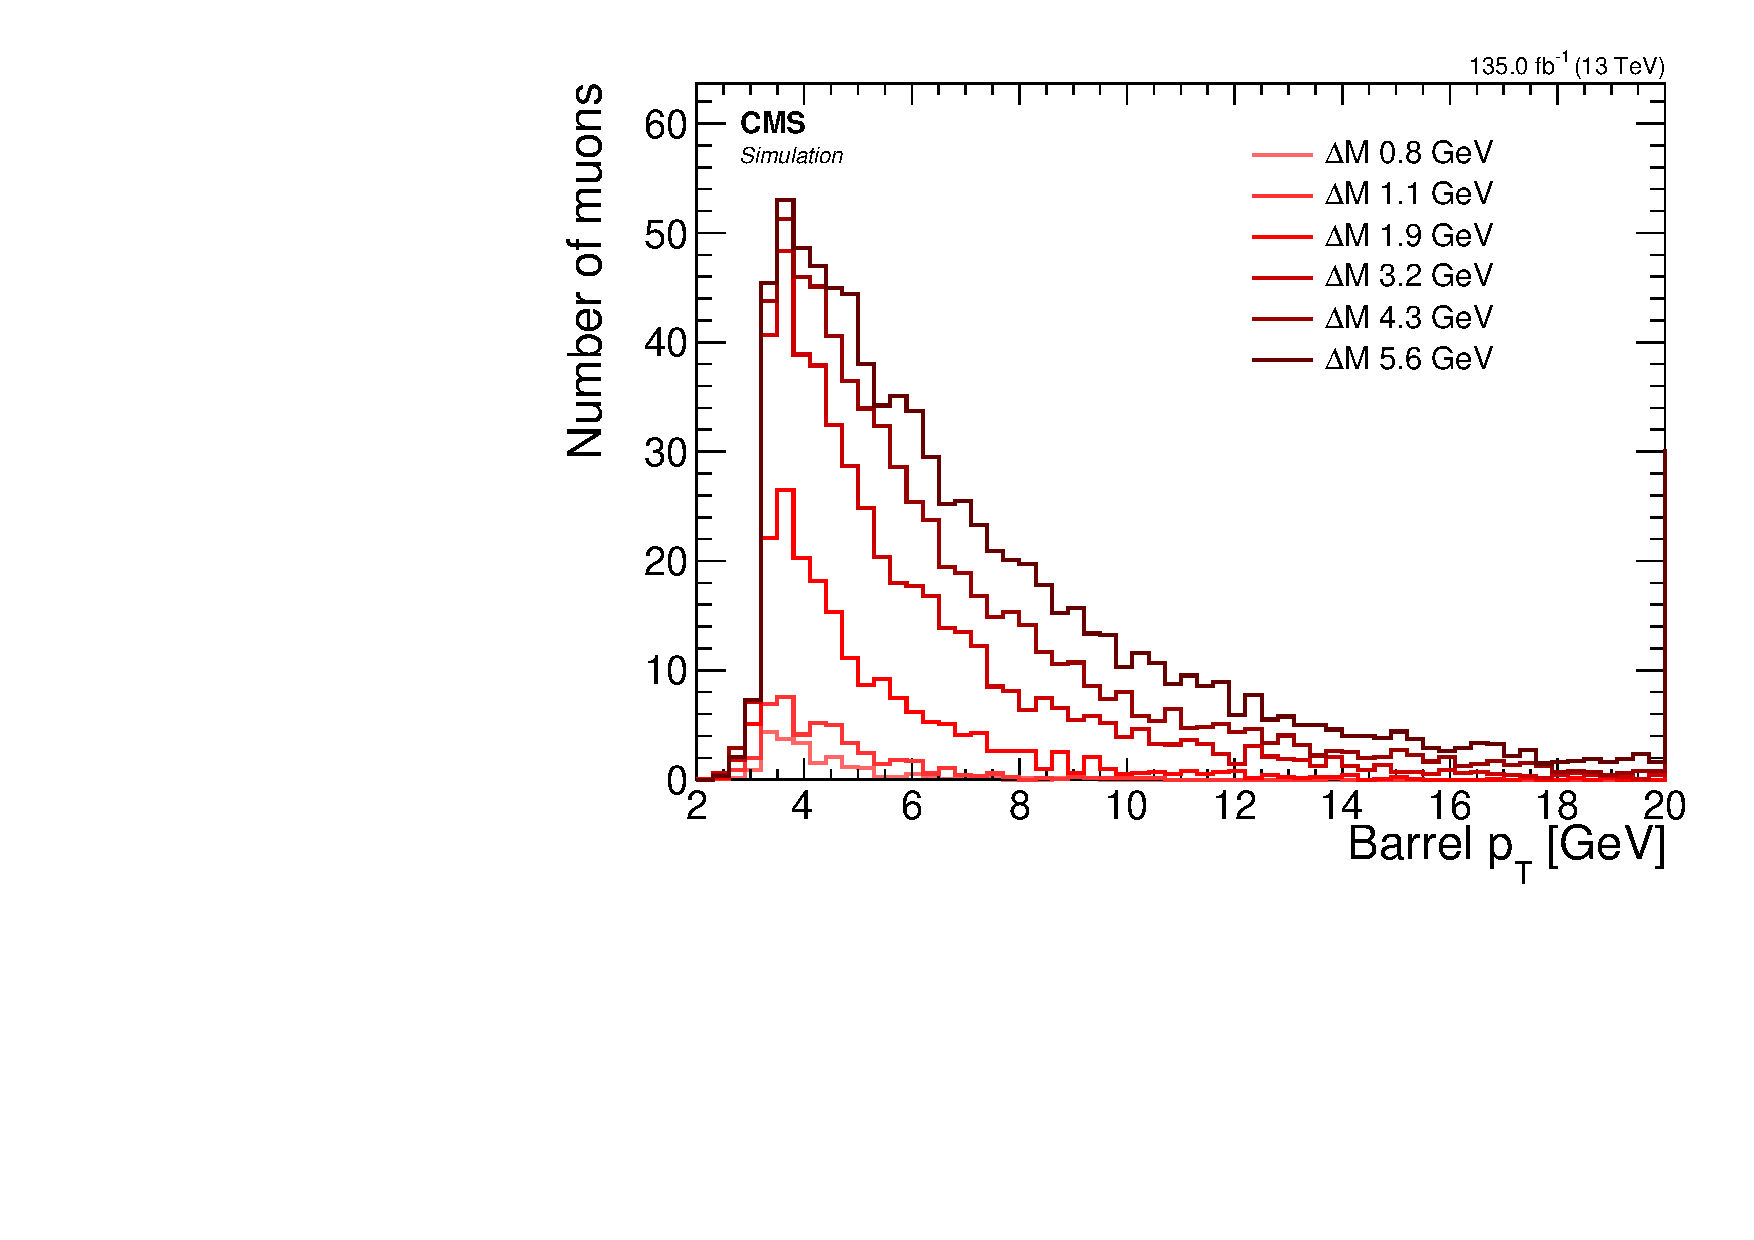
\includegraphics[width=0.48\linewidth]{plots/signal_muons/none_Muons_pt_barrel.pdf} \,
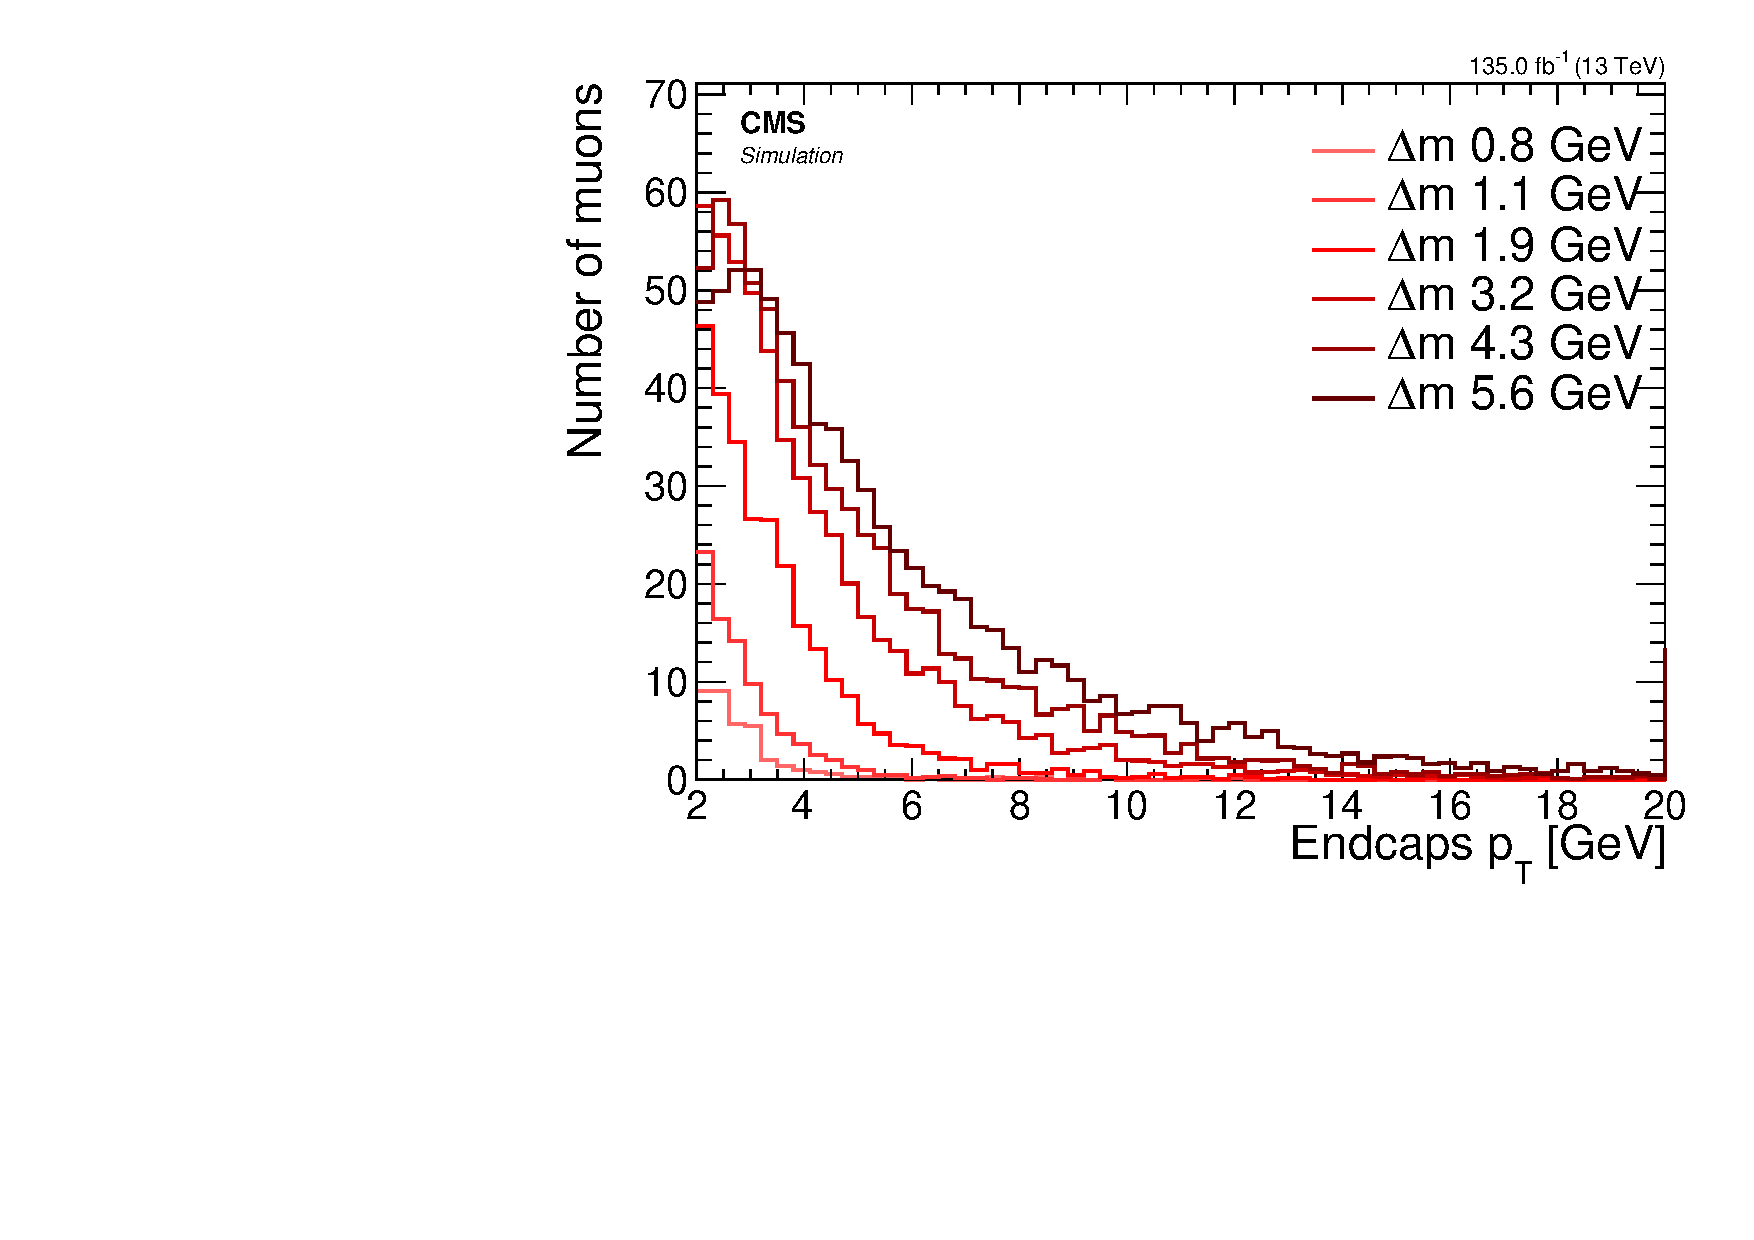
\includegraphics[width=0.48\linewidth]{plots/signal_muons/none_Muons_pt_endcape.pdf}  \\
\caption[Signal \pt distributions split into barrel and endcaps]{ Signal inclusive \pt distributions for barrel $\abs{\eta} < 1.2$ (left) and endcaps $\abs{\eta} \geq 1.2$ (right) at generator level (top) and reconstruction level passing analysis selection (bottom).}
\label{fig:signal-pt-barrel-endcaps}
\end{figure}

The picture becomes much clearer when the reconstruction efficiency as a function of \pt is examined. When comparing the generator level distribution of the barrel muons on the top left with its reconstructed counterpart on the bottom left, it can be seen that the barrel is almost completely unable to reconstruct muons with $\pt < 3\GeV$, while the endcaps, shown on the left, are able to do so. As demonstrated in the upcoming sections on \gls{mll} and \gls{dr} (see \ref{sec:gen-invariant-mass} and \ref{sec:lepton-dr}), the relationship between these distributions has consequences for the reshaping of kinematic distributions, as well as signal acceptance in general. Access to low \dm signal points is crucially dependent on the low \pt region of $2 \leq \pt \leq 3.5\GeV$, which is mainly achieved with the help of the muon chamber endcaps, as can be seen here.

Since the barrel and endcaps are seperated by different regions of $\eta$, $\abs{\eta} < 1.2$ for barrel and $\abs{\eta} \geq 1.2$ for endcaps, it is worthwhile taking a look at the $\eta$ distributions of the muons as well. Those can be seen at Figure~\ref{fig:signal-muons-eta}.

\begin{figure}[!htb]
\centering
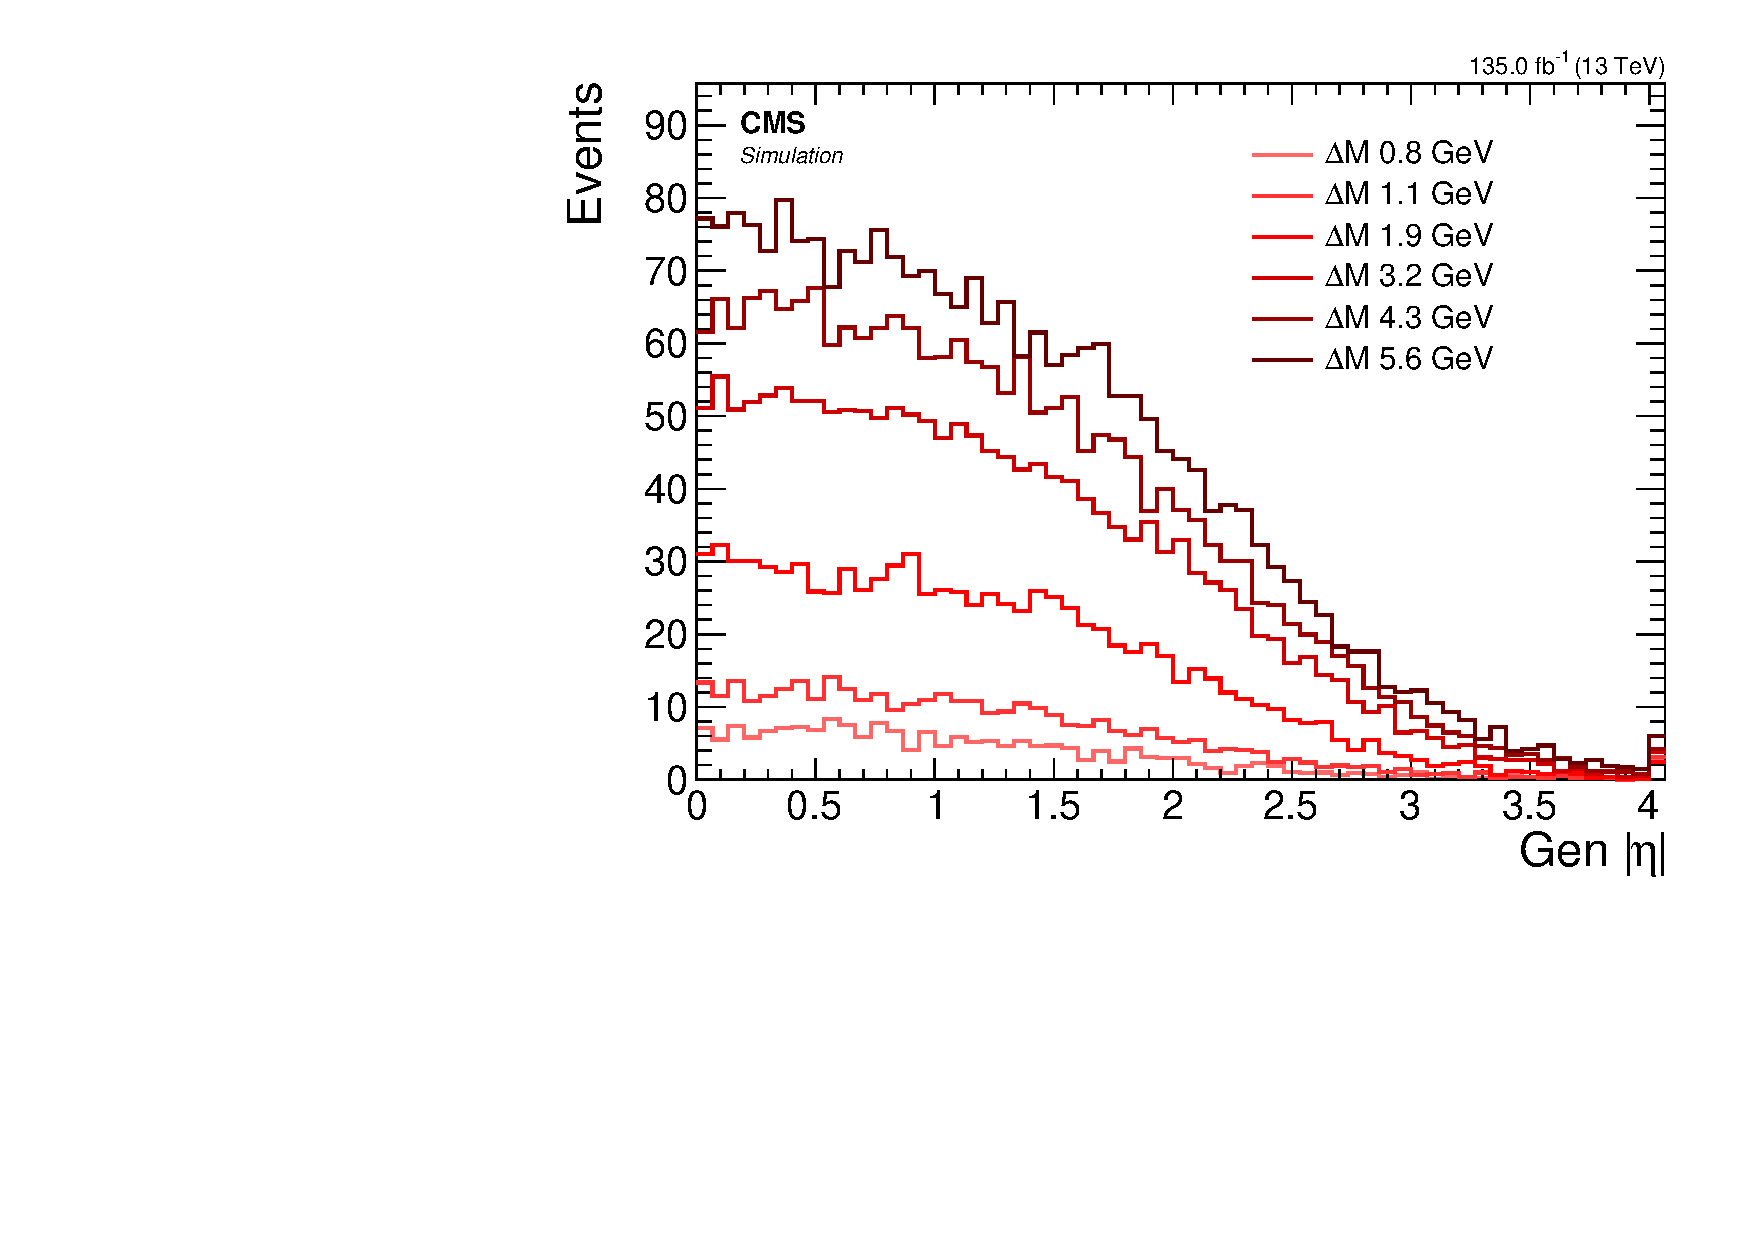
\includegraphics[width=0.32\linewidth]{plots/signal_muons_gen/none_Muons_Eta.pdf} \,
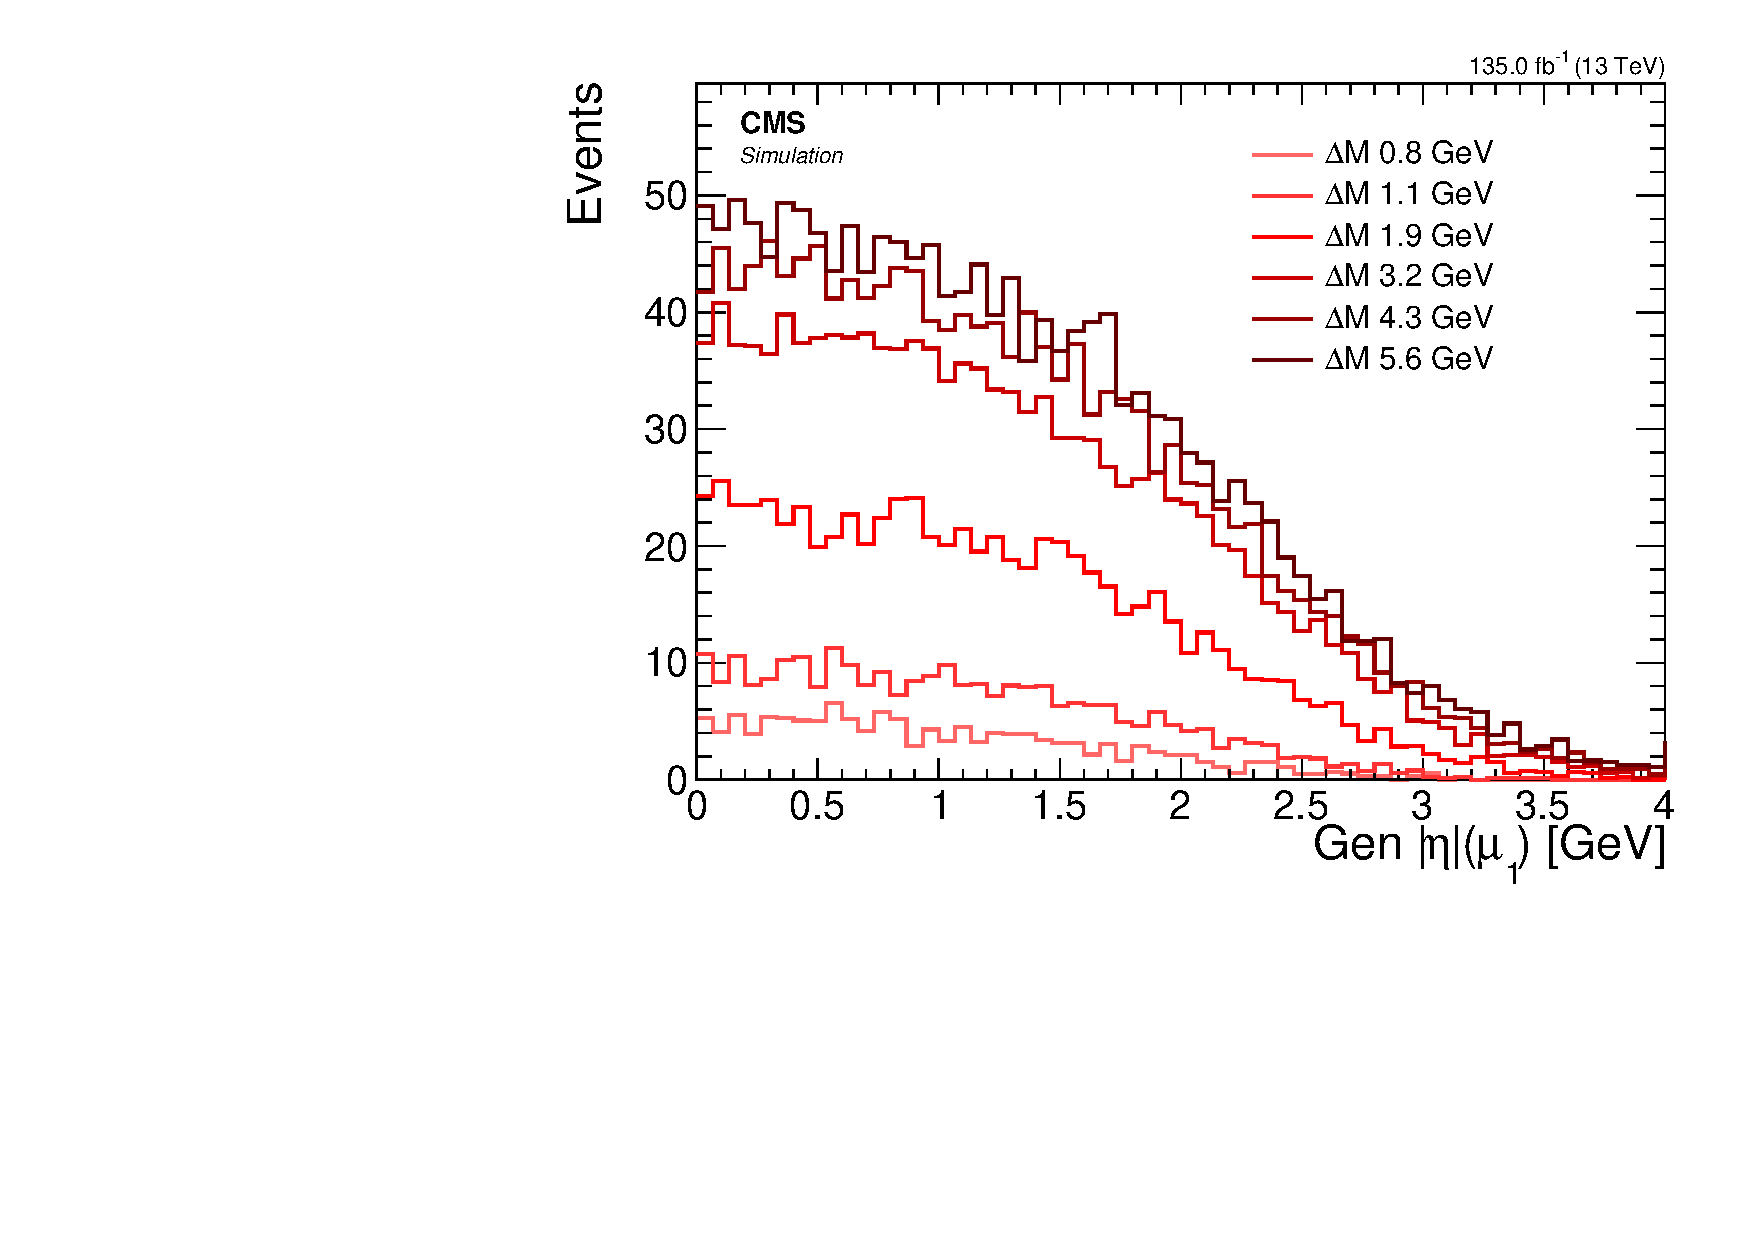
\includegraphics[width=0.32\linewidth]{plots/signal_muons_gen/none_Muons_m1_eta.pdf}  \,
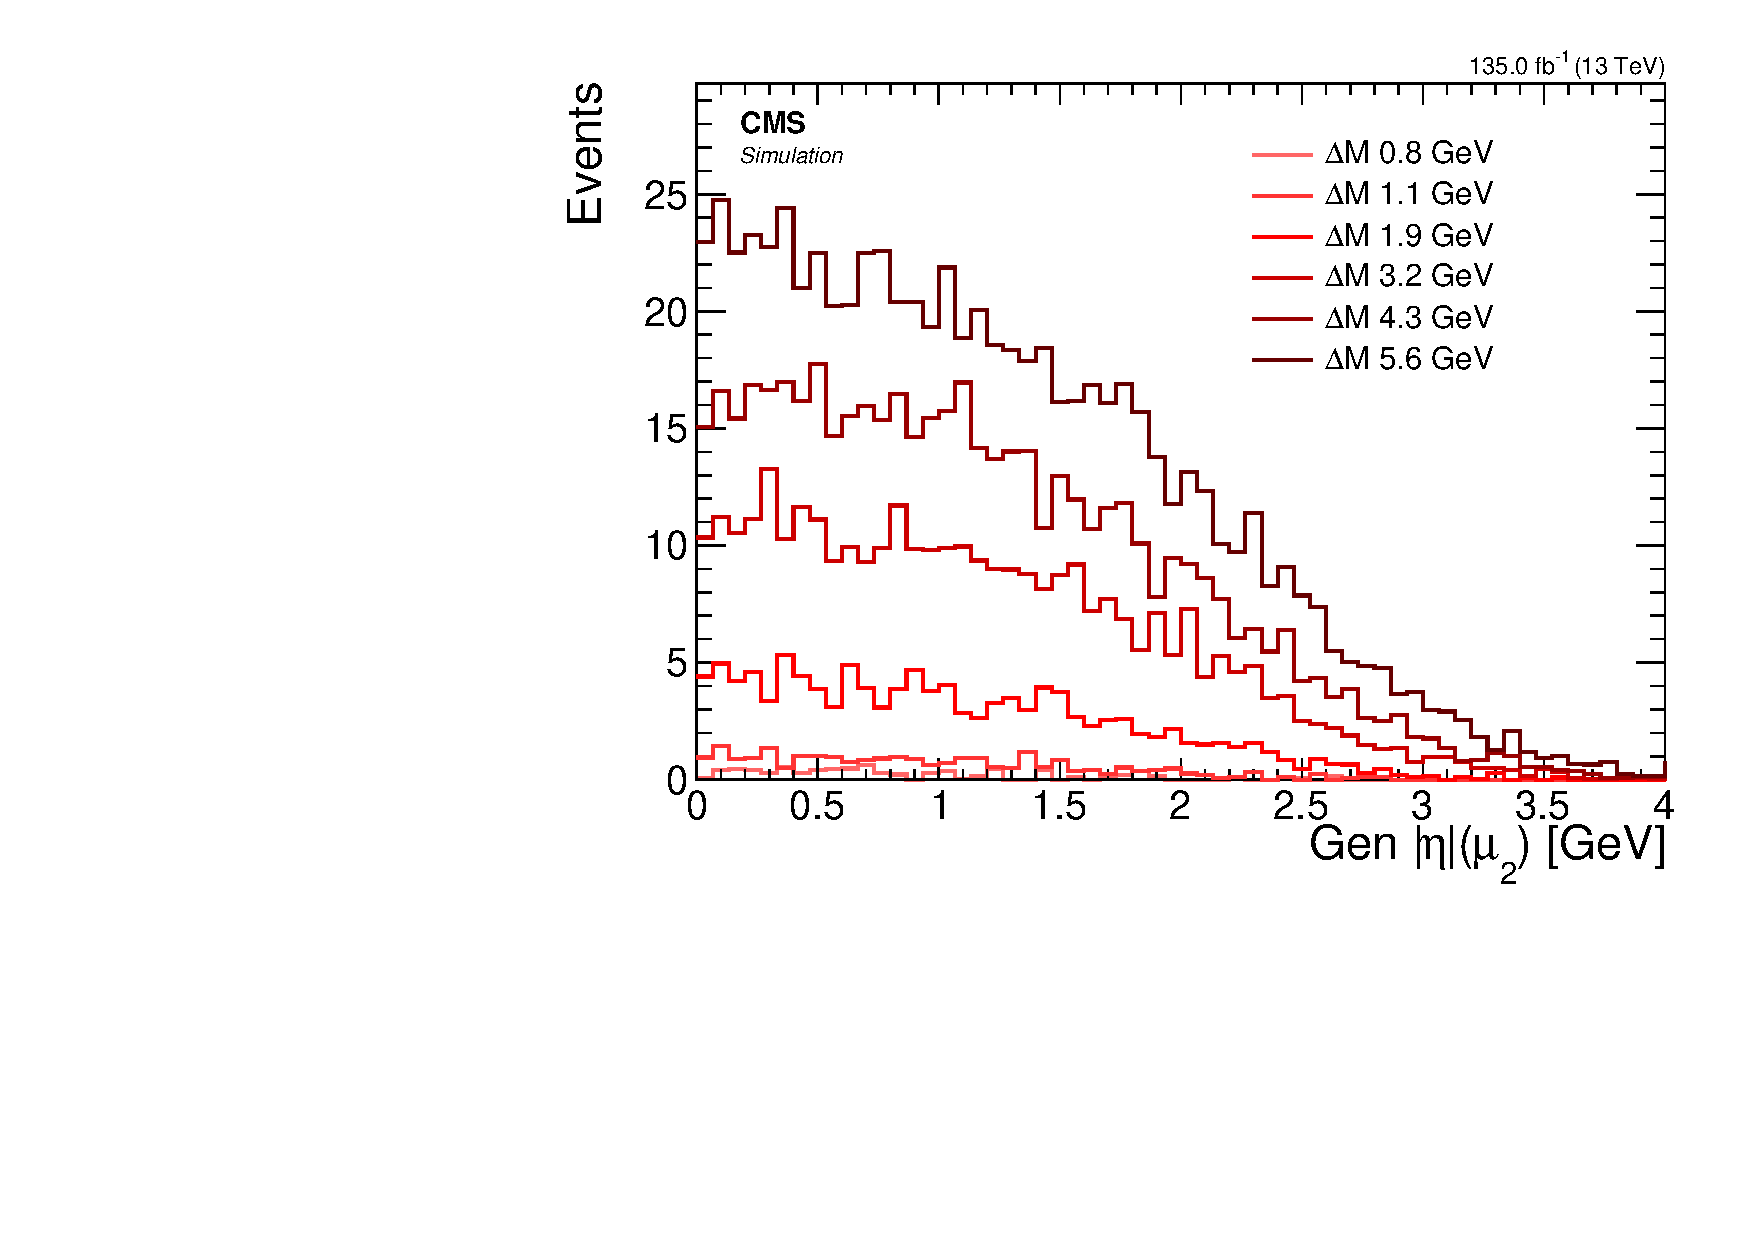
\includegraphics[width=0.32\linewidth]{plots/signal_muons_gen/none_Muons_m2_eta.pdf} \\
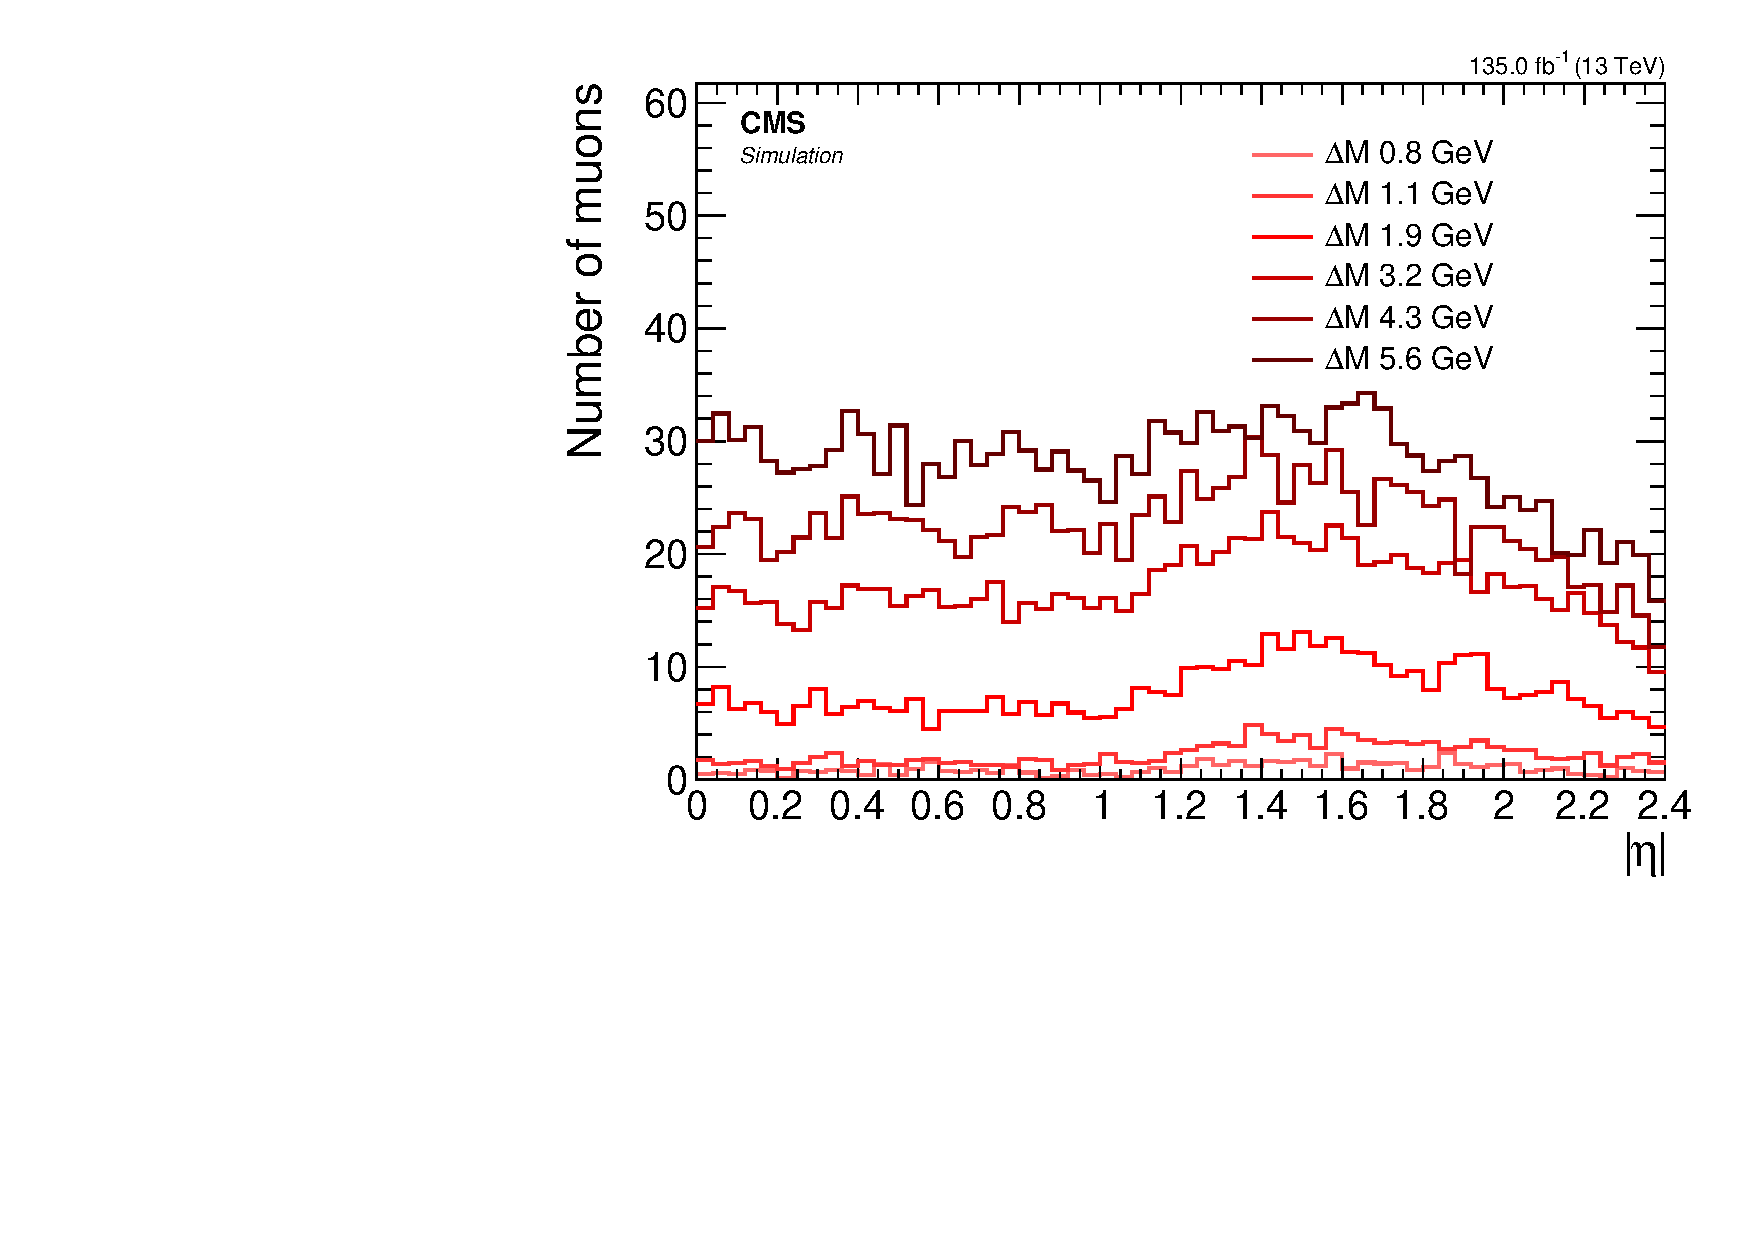
\includegraphics[width=0.32\linewidth]{plots/signal_muons/none_Muons_Eta.pdf} \,
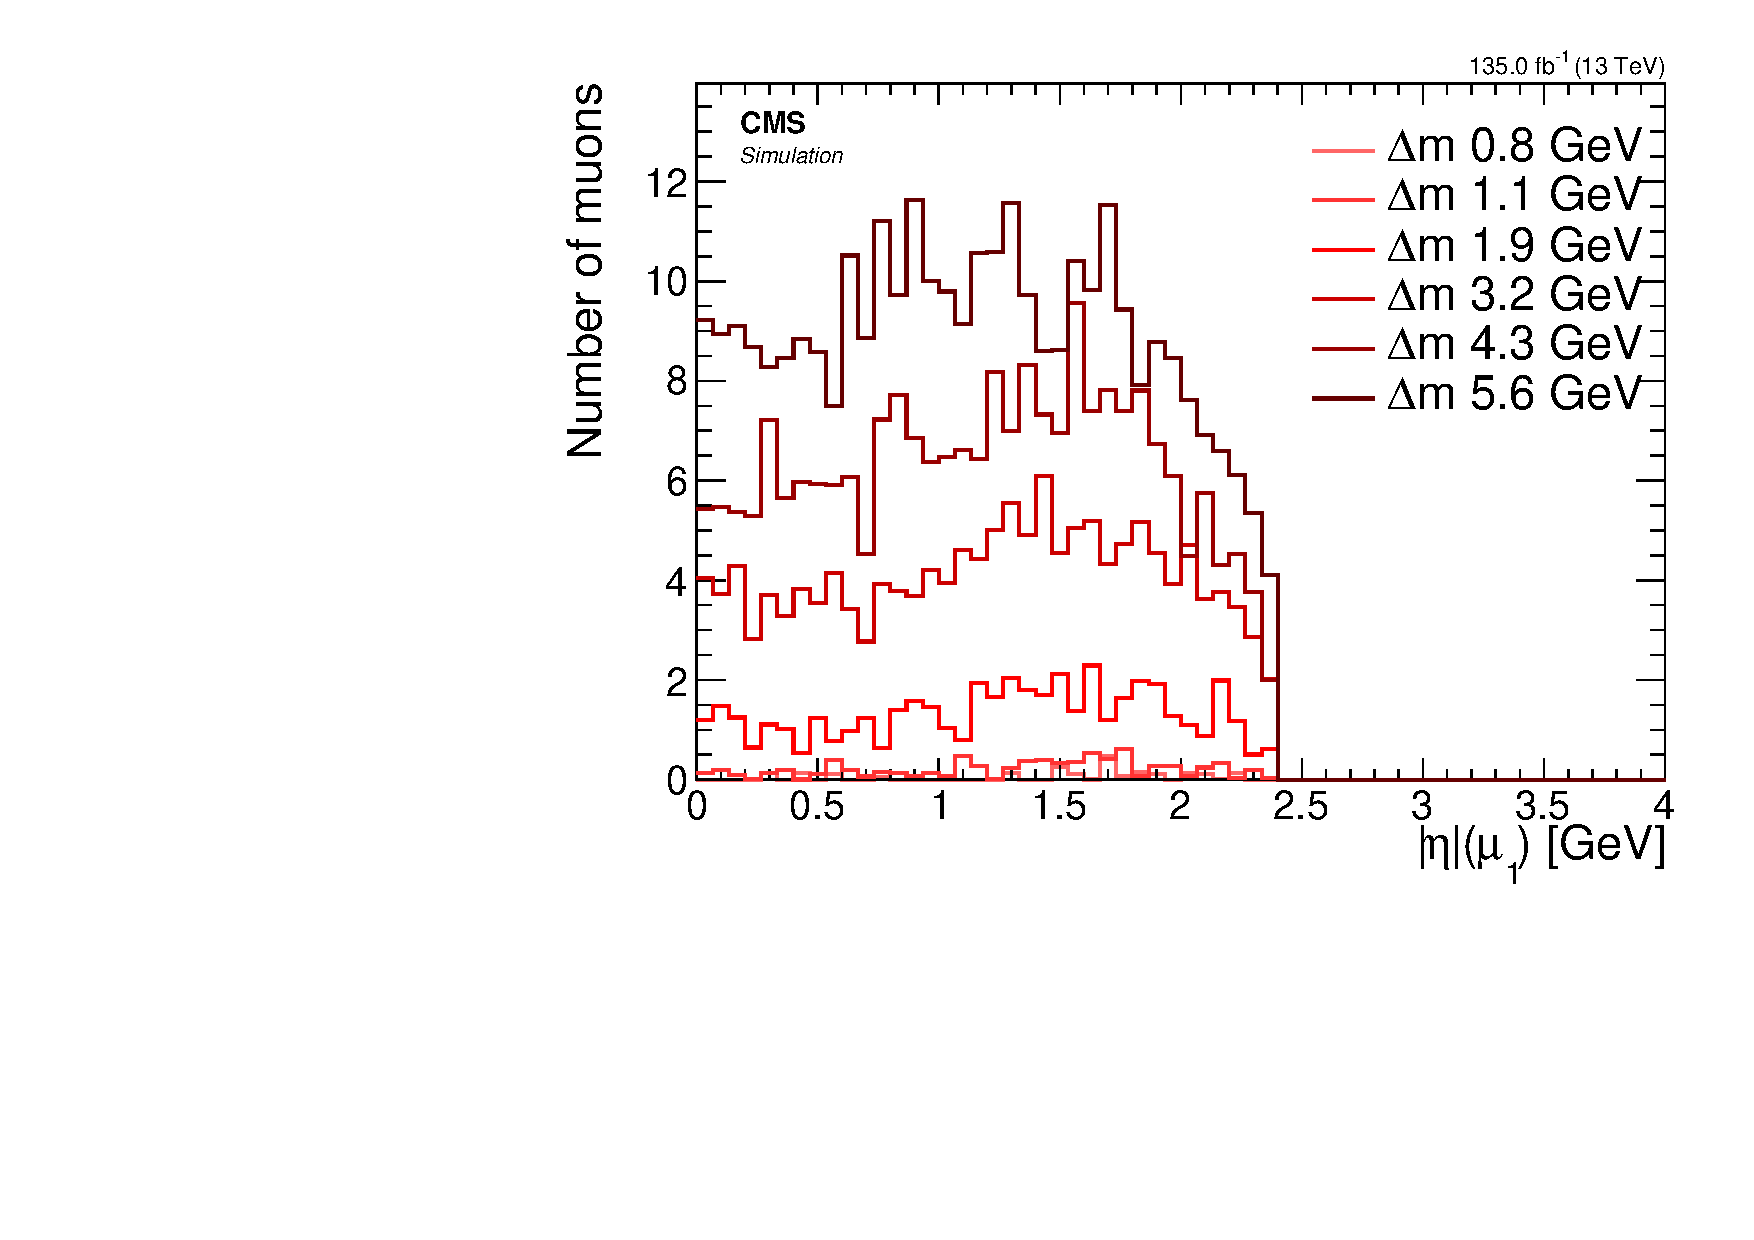
\includegraphics[width=0.32\linewidth]{plots/signal_muons/none_Muons_m1_eta.pdf}  \,
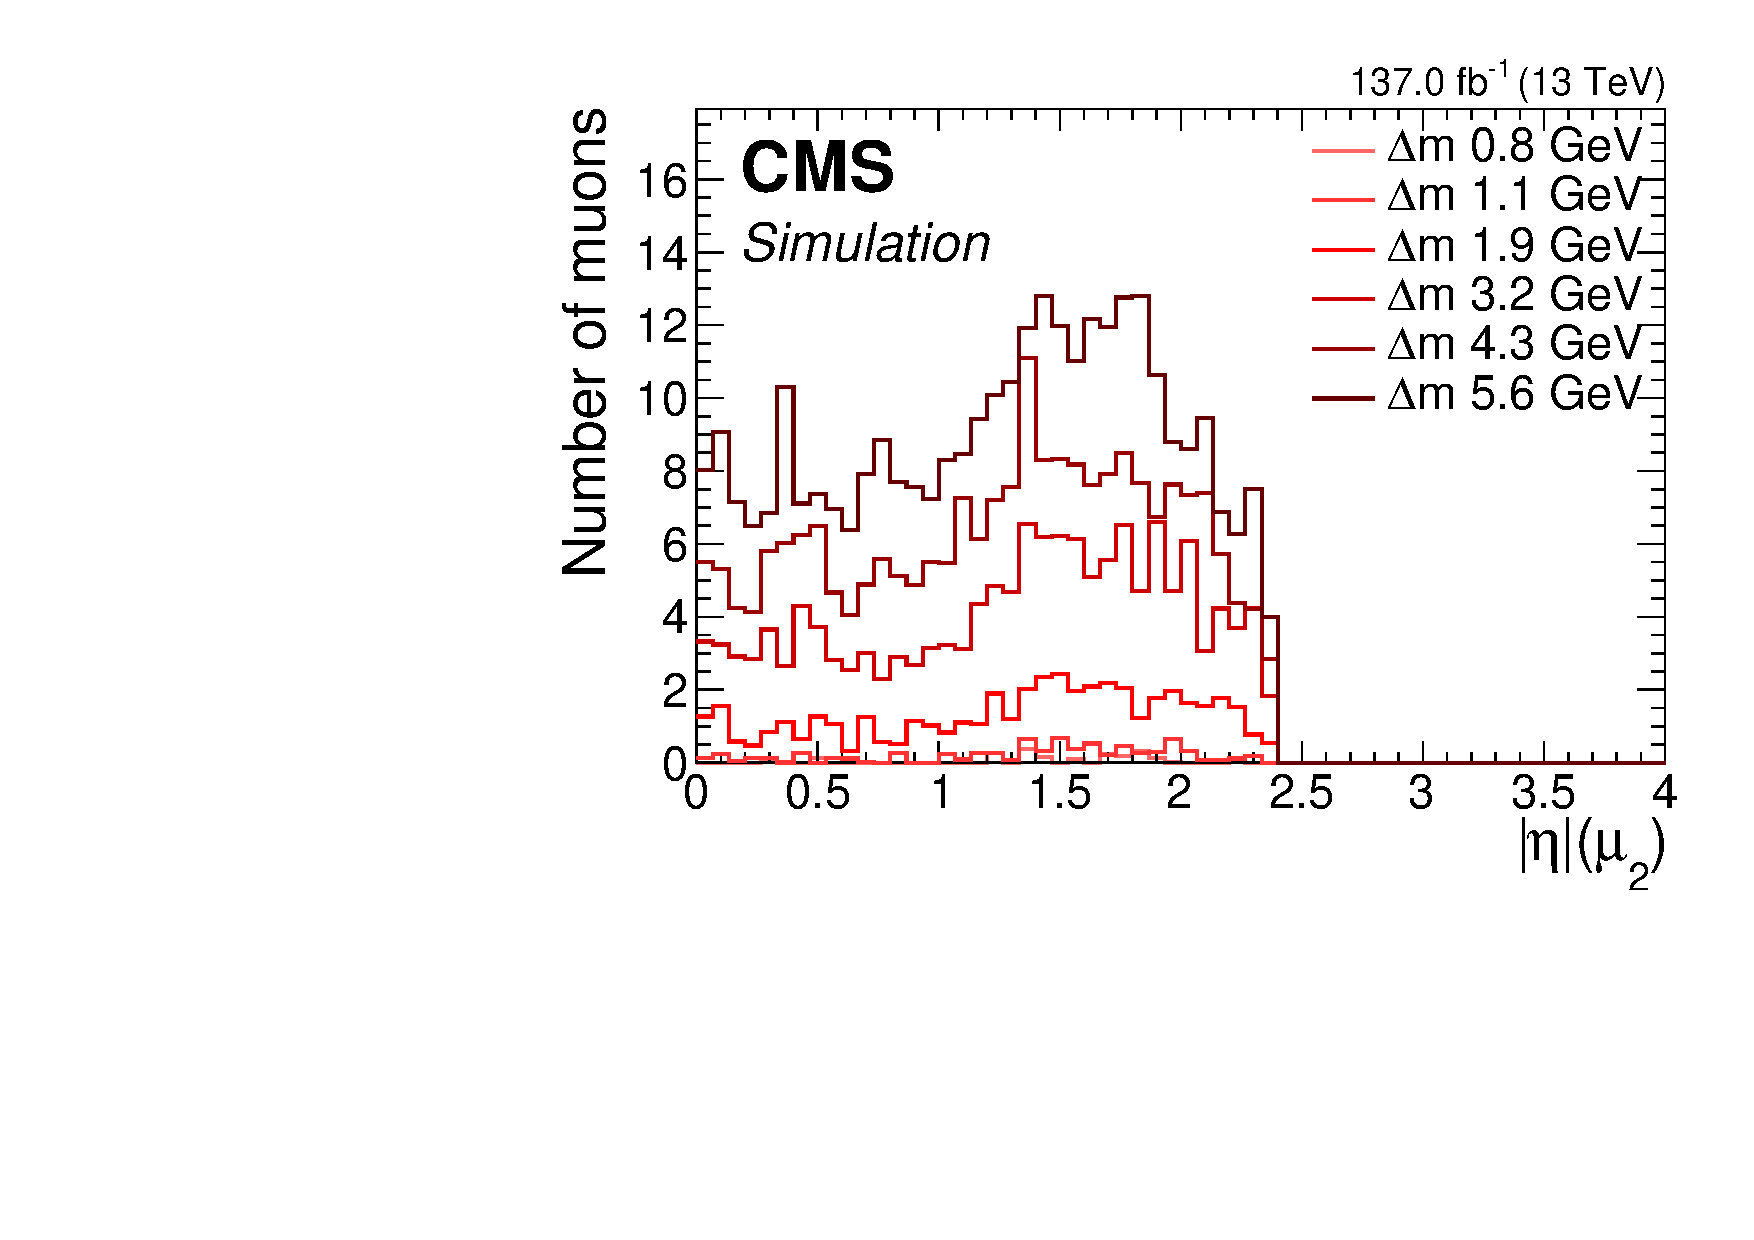
\includegraphics[width=0.32\linewidth]{plots/signal_muons/none_Muons_m2_eta.pdf} \\
\caption[Signal $\abs{\eta}$ distributions]{ Signal $\abs{\eta}$ distributions for inclusive (left), leading muon $\mu_1$ (middle),  subleading muon $\mu_2$ (right) at generator level (top) and reconstruction level passing analysis selection (bottom). }
\label{fig:signal-muons-eta}
\end{figure}

The muons analysis selection only selects muons within the tracker range of $\abs{\eta}<2.4$. This is why the muons with $\abs{\eta}>2.4$ are not present in the reconstruction plots on the bottom. It can be seen that the main effect of going from the inclusive $\abs{\eta}$ at the generator level to the reconstructed counterpart is the flattening of the distribution due to the loss of muons with $\abs{\eta}<1.2$ in the barrel for muons with $\pt<3\GeV$.

With the understanding of the reconstruction effects on the \pt and $\eta$ distributions of the muons, an examination of other kinematic variables of the dilepton system is now possible.

\clearpage

\subsubsection{Invariant mass \gls{mll}}
\label{sec:gen-invariant-mass}

The invariant mass of the two leptons resulting from the decay of the \neutt has a unique shape due to the limited allowed phase space of the leptons as part of the 3-body decay. As the \neutt decays into \neuto and \ellell through a \PZstar, the allowed phase space of the dilepton pair is restricted to the mass difference between \neutt and \neuto, that is, \dm. Therefore, the \gls{mll} distribution is expected to have an edge at \dm. Distributions of the generator level invariant mass can be seen in Figure~\ref{fig:signal-generator-mll}.

\begin{figure}[!htb]
\centering
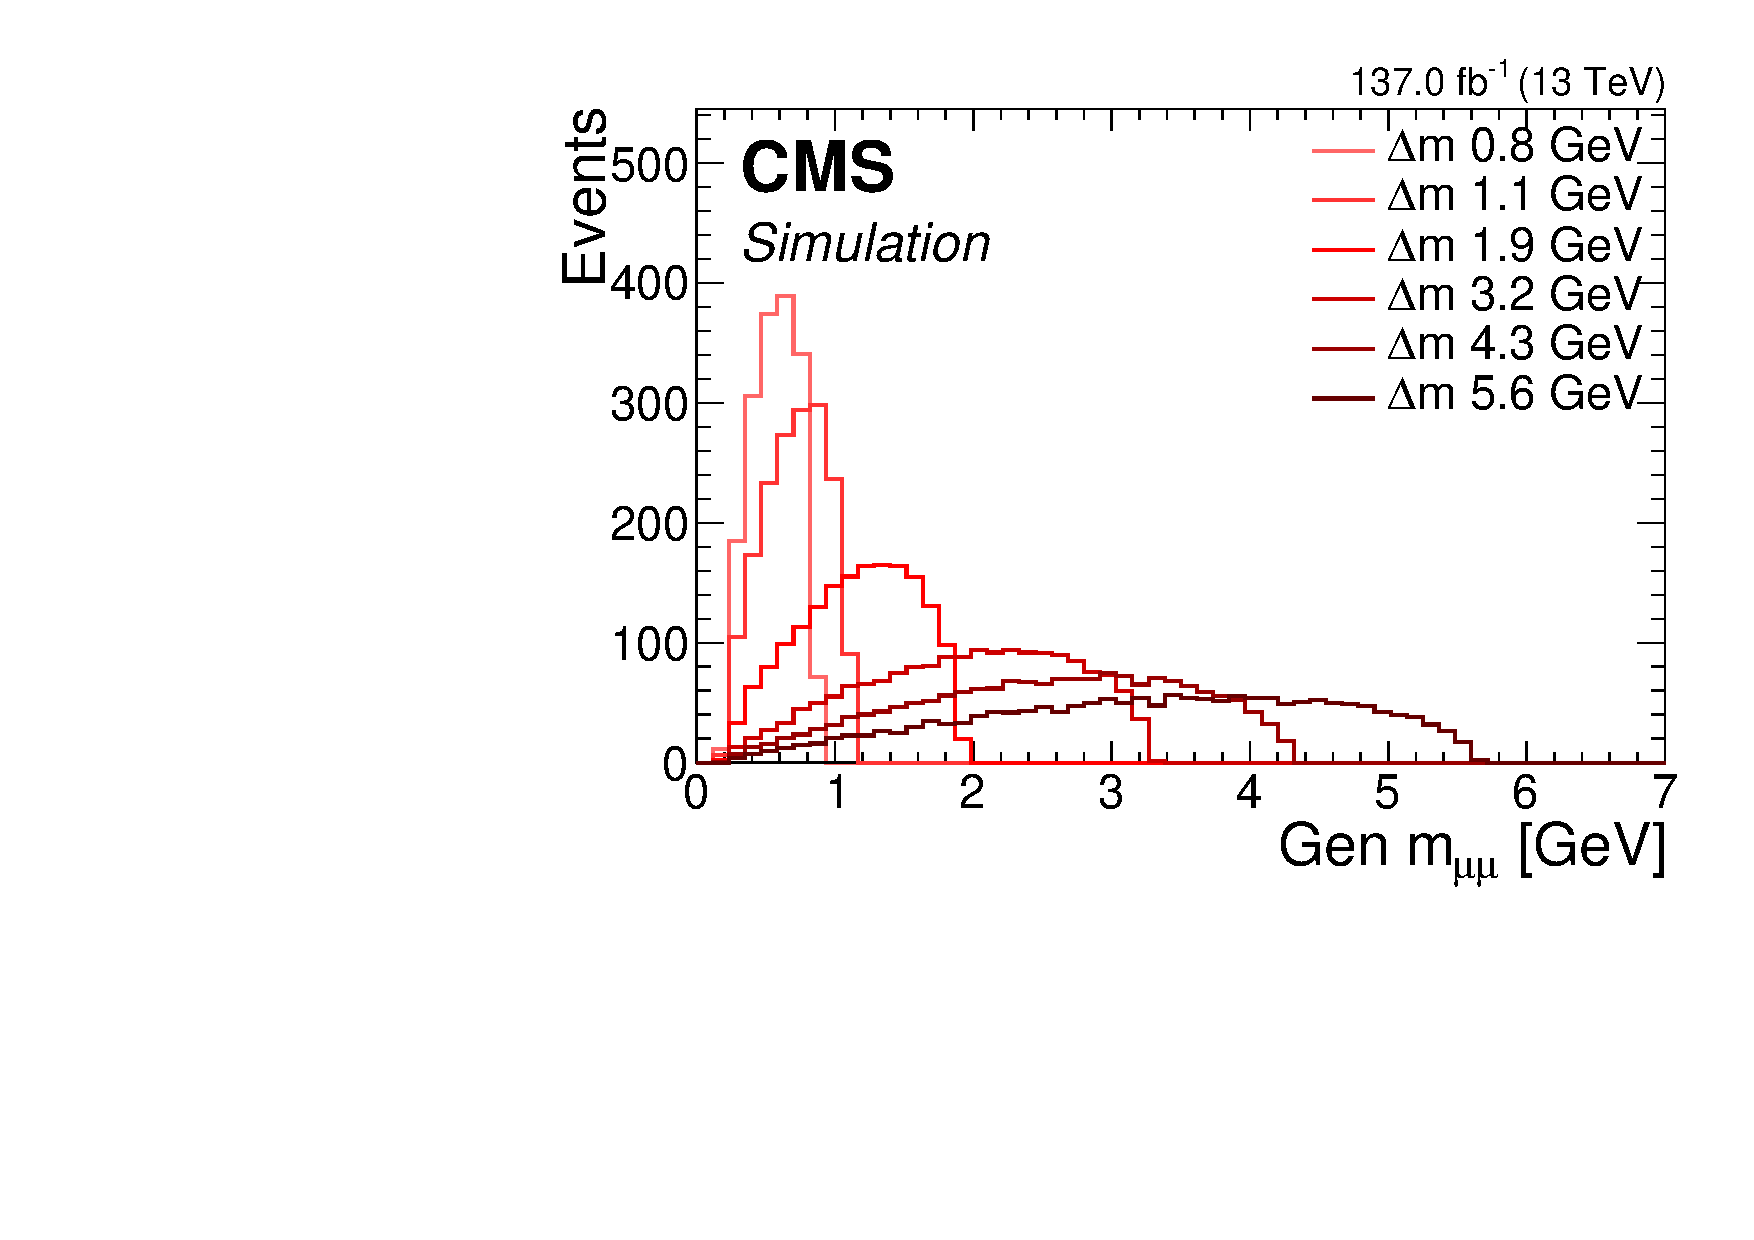
\includegraphics[width=0.32\linewidth]{plots/signal_muons_gen/none_gen_invMass.pdf} \,
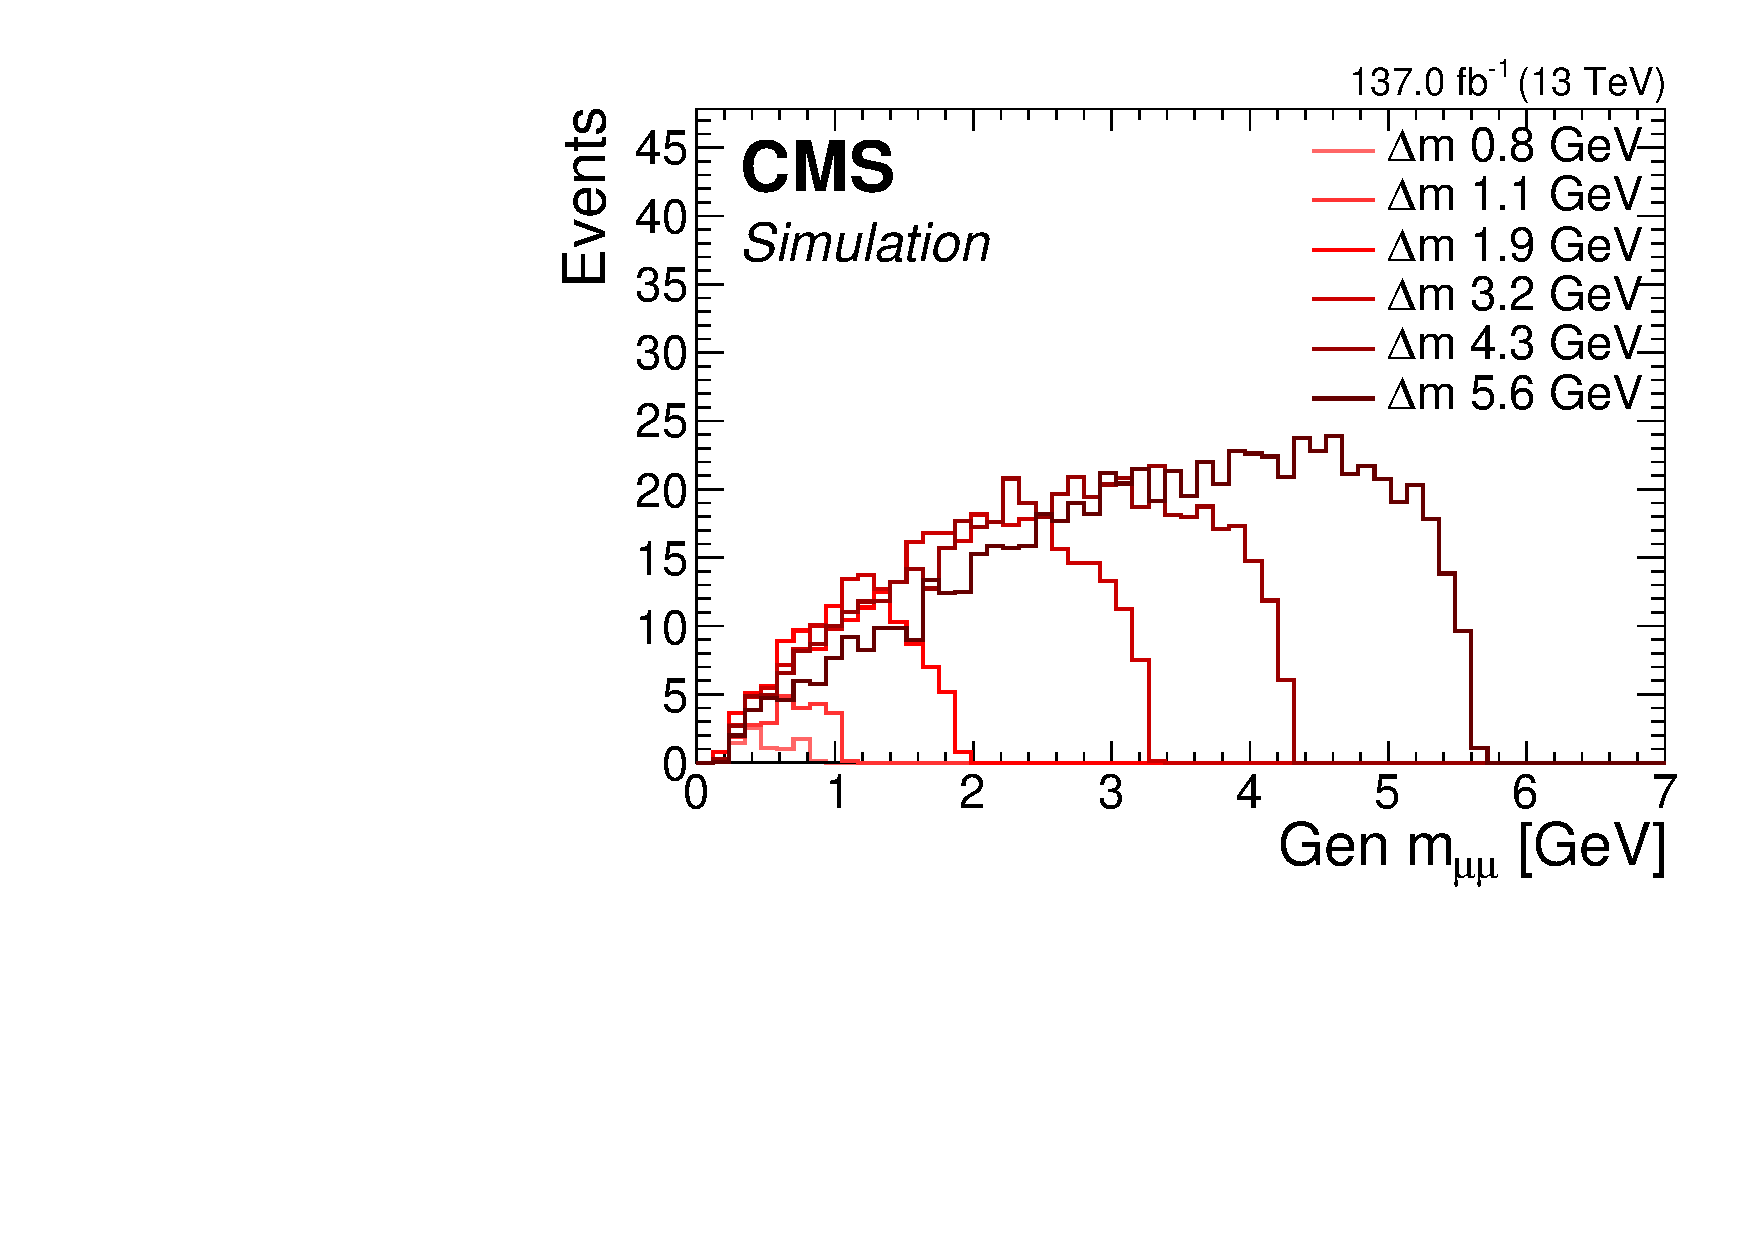
\includegraphics[width=0.32\linewidth]{plots/signal_muons_gen/none_gen_invMass_cut.pdf}  \,
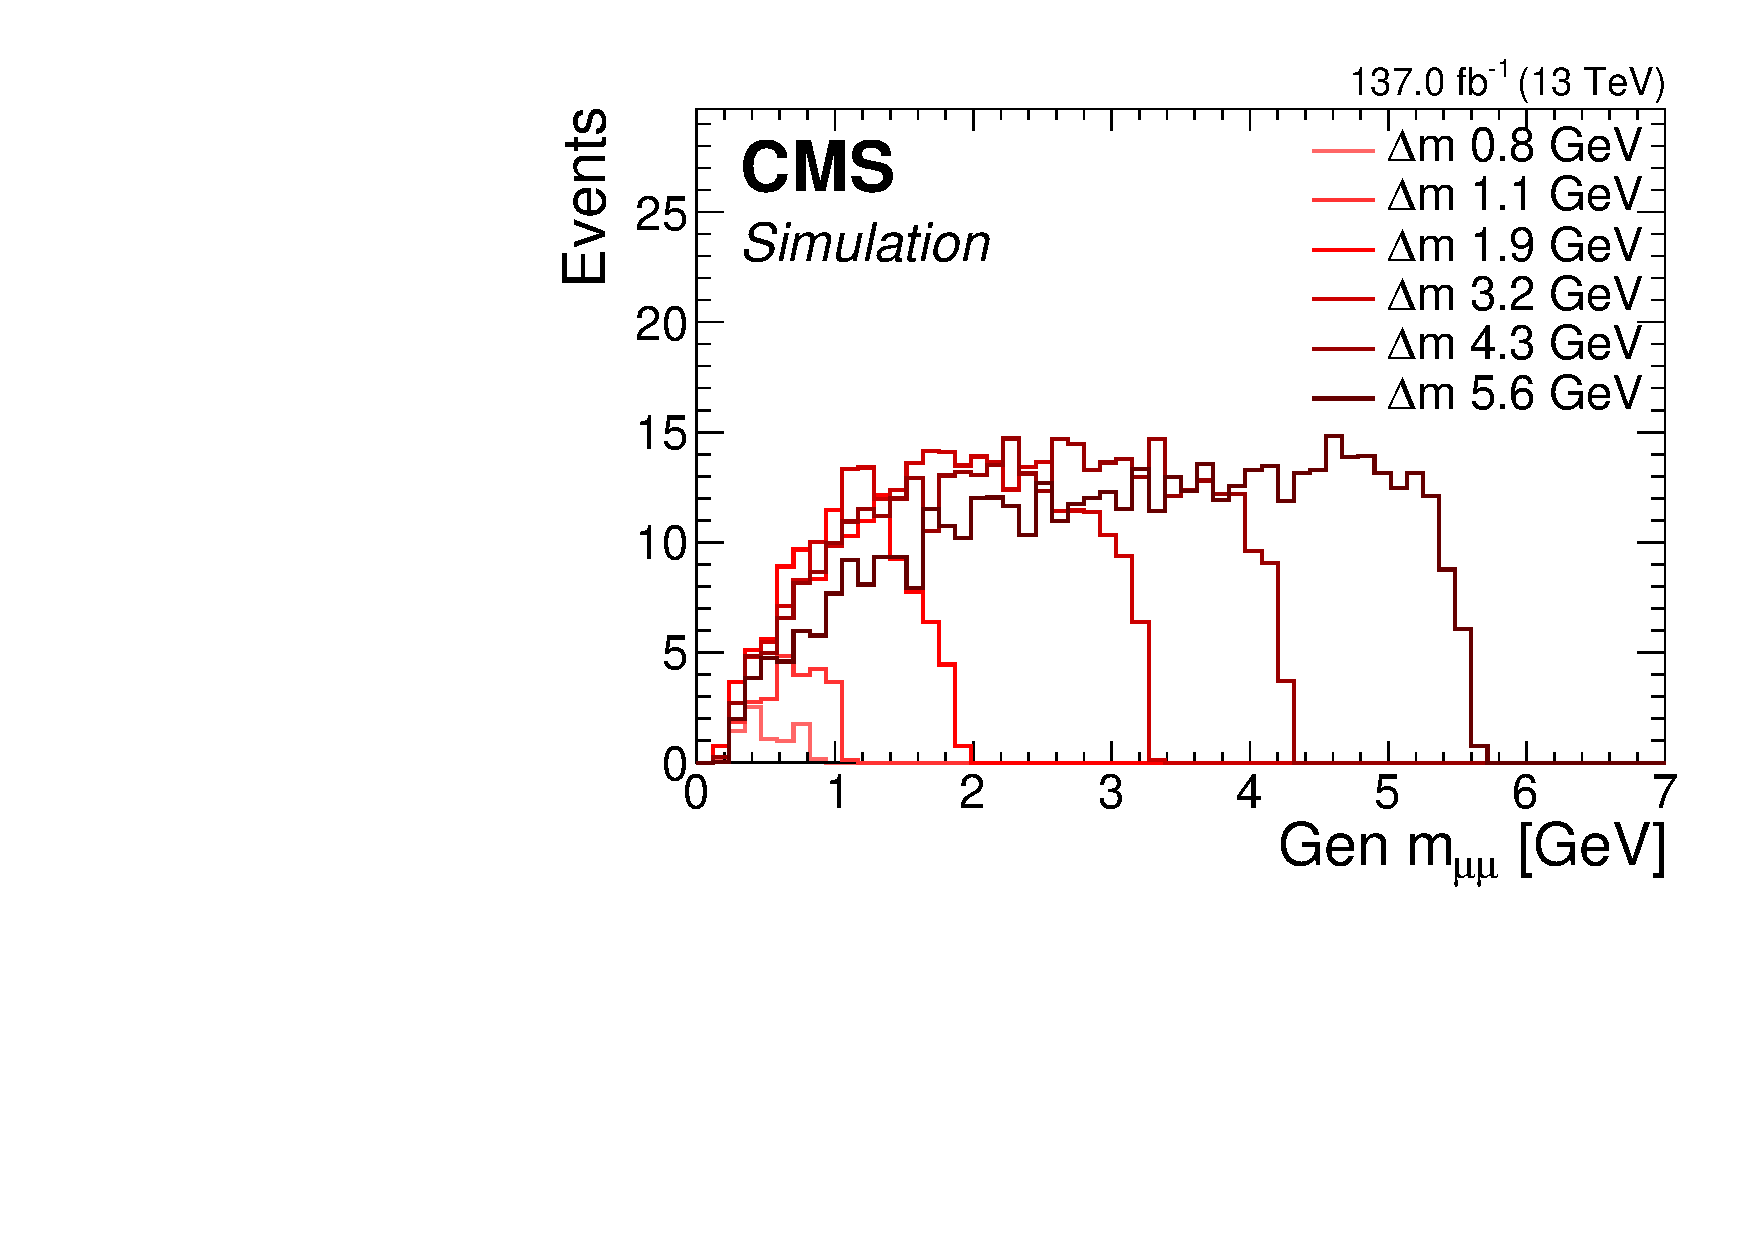
\includegraphics[width=0.32\linewidth]{plots/signal_muons_gen/none_gen_invMass_orth.pdf} \\
\caption[Signal generator level \mll distributions]{ Signal generator level \mll distributions with no cuts (left), with $\pt\left(\mu_i\right)>2\GeV,\,i=1,2$ (middle) and with \gls{sos} orthogonality condition $\pt\left(\mu_i\right)>2\GeV$, $\pt\left(\mu_2\right)\leq~3.5\GeV\text{ or }\Delta R\leq 0.3$ (right).}
\label{fig:signal-generator-mll}
\end{figure}

The inclusive distribution of the invariant mass of the muons \mmumu is shown on the left. The edge of the \mmumu distribution for each signal point is located right at the corresponding \dm. However, when the muons \pt are cut and required to be $\pt\geq 2\GeV$, the shape of the distribution shifts, and the efficiency in the lower \dm range drops significantly, as depicted in the middle plot. Lastly, the effect of orthogonalizing phase space to the \gls{sos} analysis is demonstrated in the rightmost plot. The effect is strongest in high \dm and quite subtle in low \dm.

To comprehend the reshaping that occurs to the \mmumu shape, the relationship between the \pt of the muons (leading muon denoted $\mu_1$ while subleading muon is denoted $\mu_2$) and the invariant mass is examined. One signal with low \dm of $1.13\GeV$ and one with high \dm of $5.63\GeV$ are selected for this analysis. The distributions are shown in Figure~\ref{fig:signal-gen-invamass-pt}.

\begin{figure}[!htb]
\centering
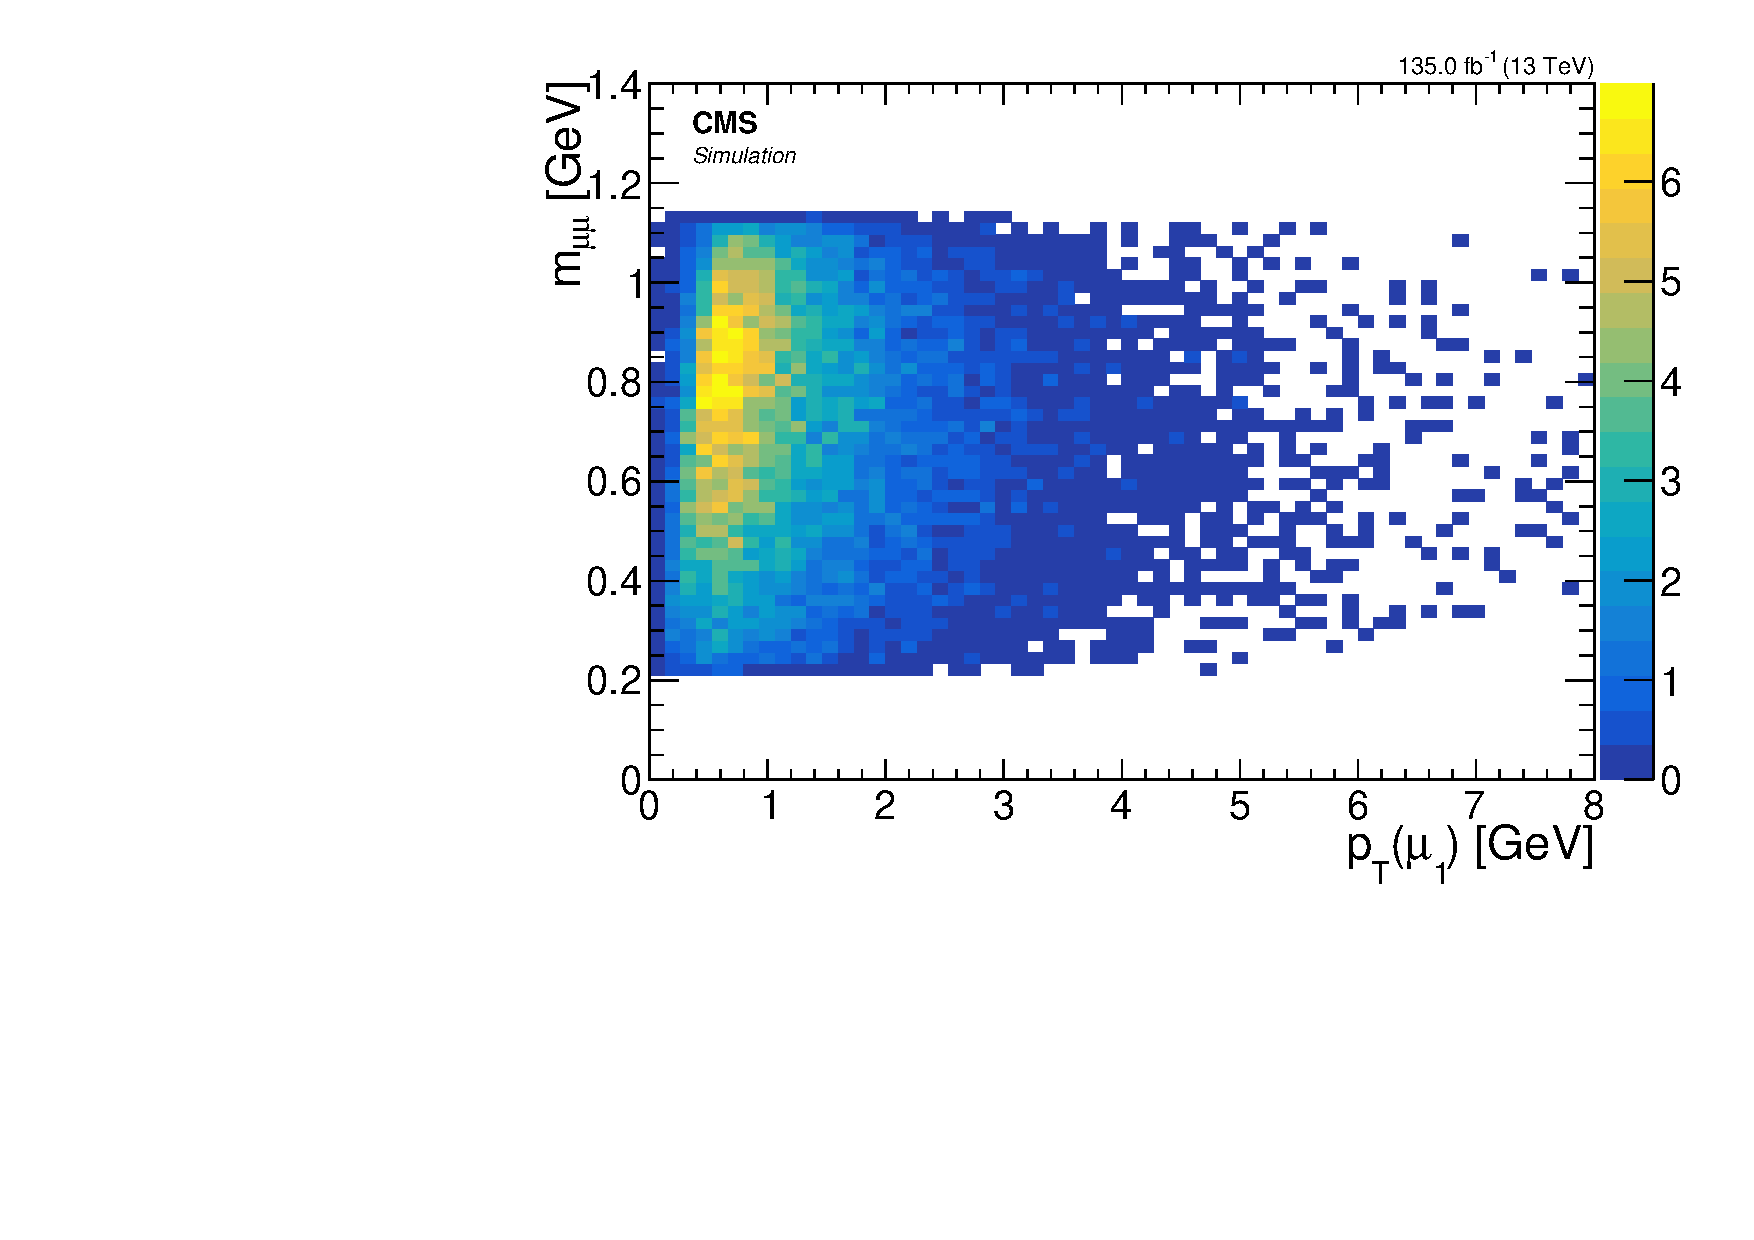
\includegraphics[width=0.48\linewidth]{plots/signal_muons_gen_delta_r_vs_pt/none_gen_invmass_vs_pt_1.pdf} \,
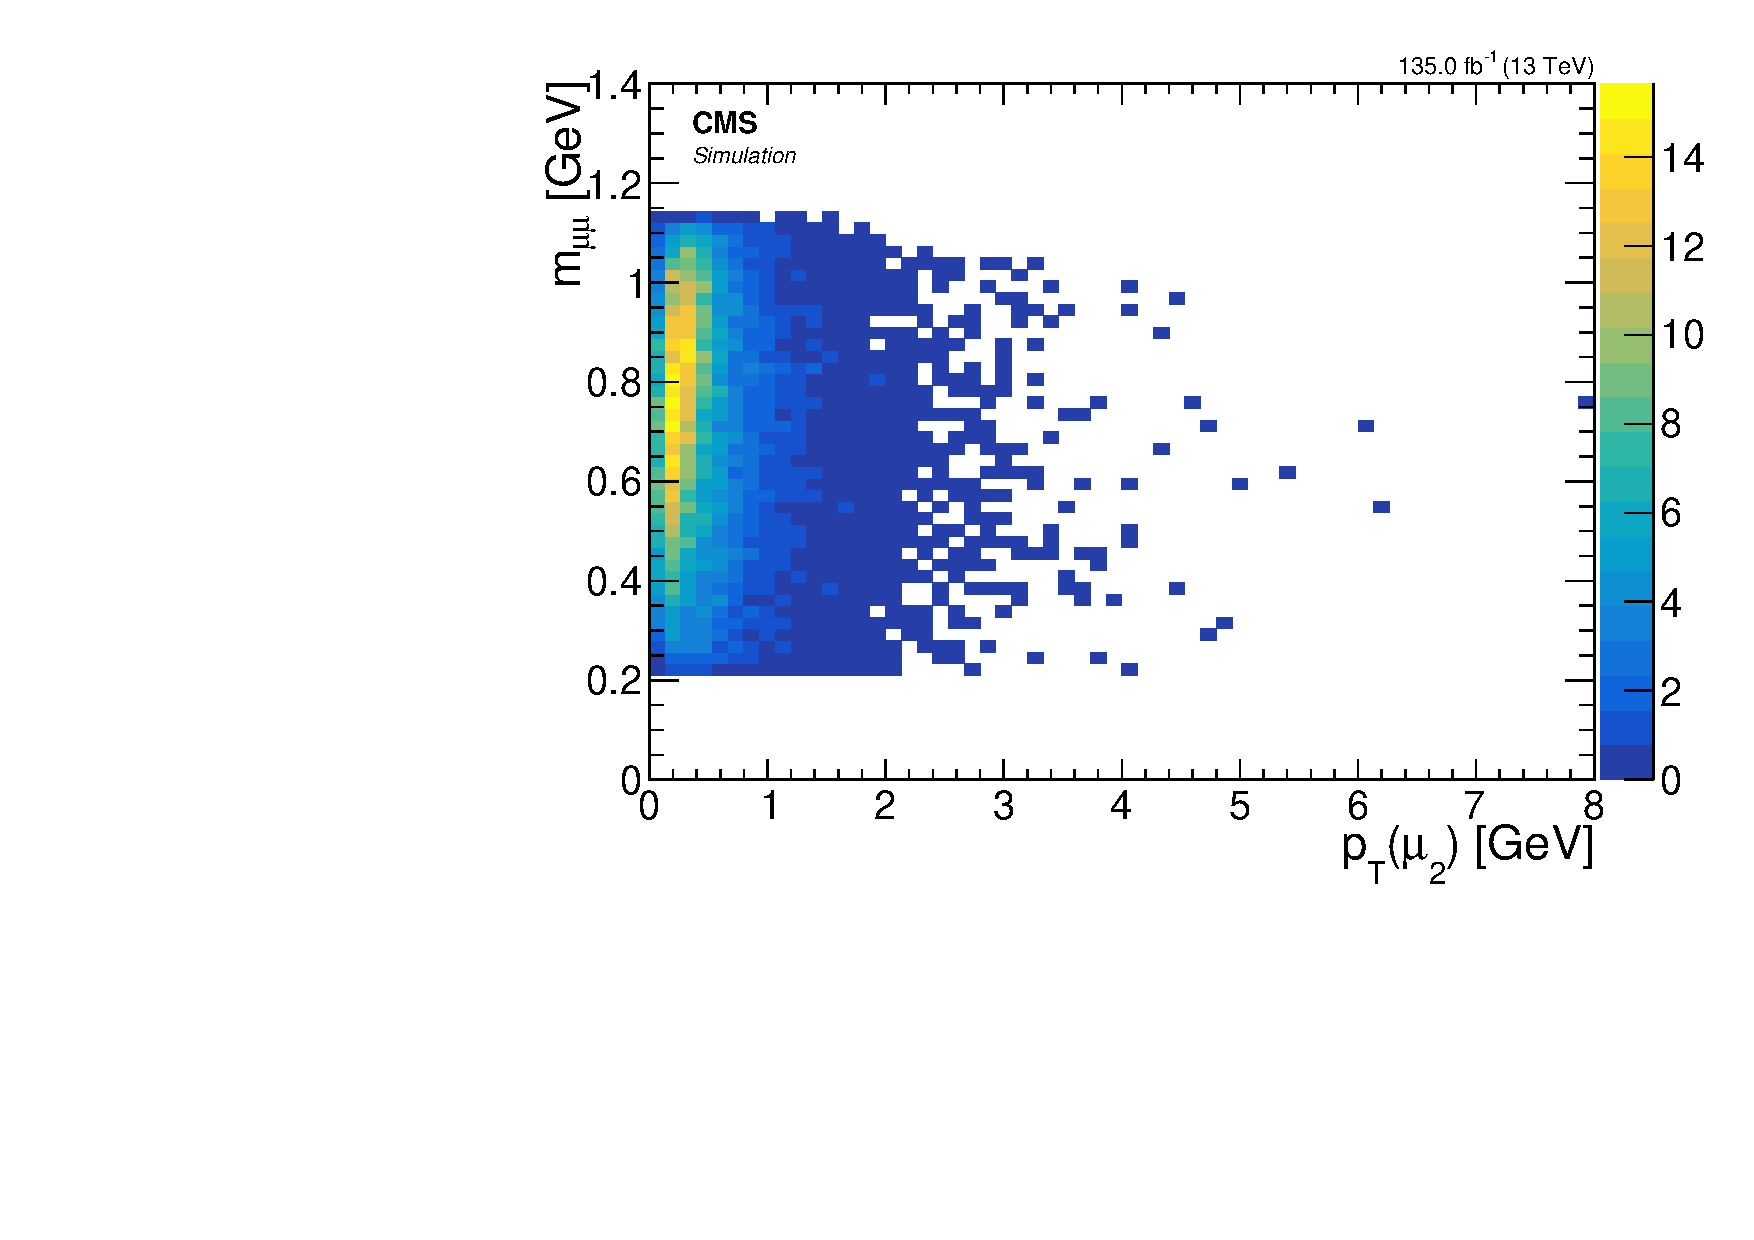
\includegraphics[width=0.48\linewidth]{plots/signal_muons_gen_delta_r_vs_pt/none_gen_invmass_vs_pt_2.pdf}  \\
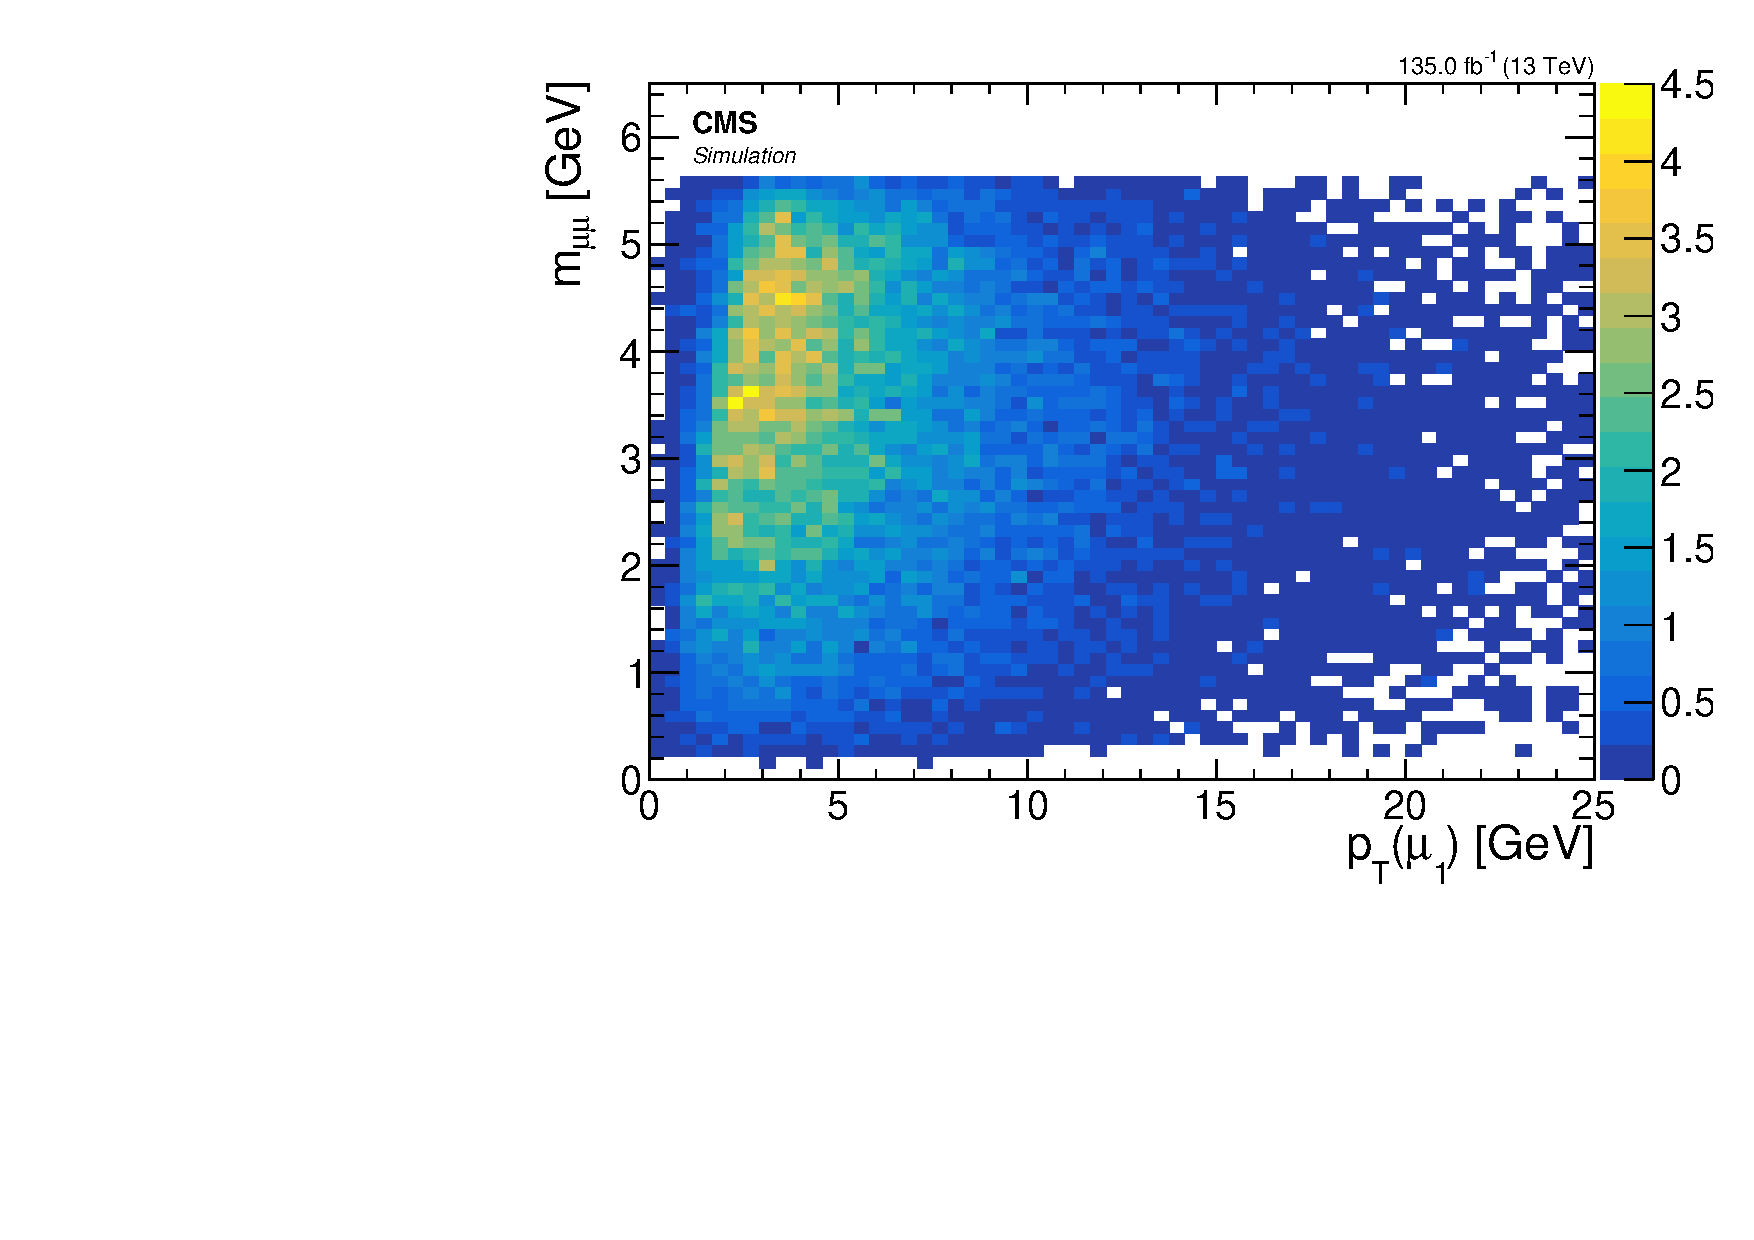
\includegraphics[width=0.48\linewidth]{plots/signal_muons_gen_delta_r_vs_pt_dm5/none_gen_invmass_vs_pt_1.pdf} \,
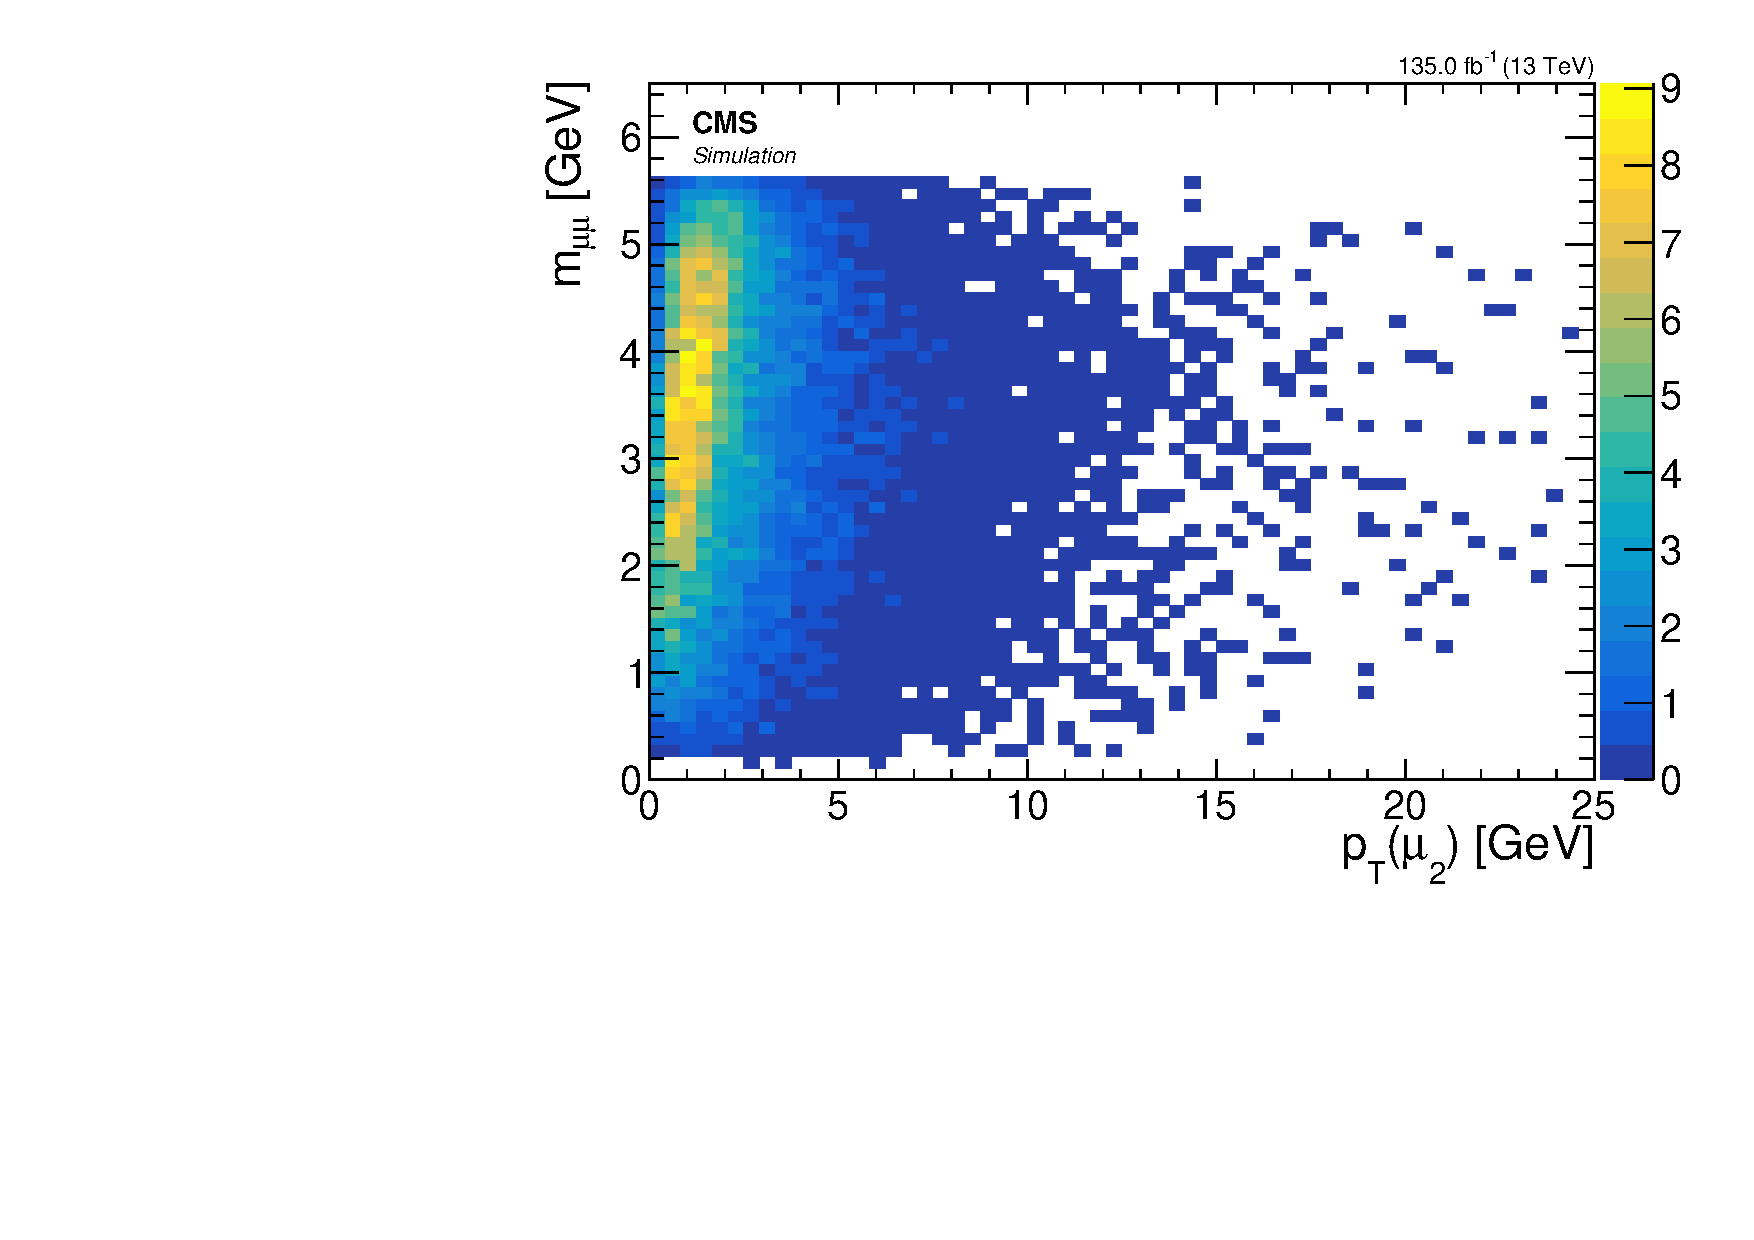
\includegraphics[width=0.48\linewidth]{plots/signal_muons_gen_delta_r_vs_pt_dm5/none_gen_invmass_vs_pt_2.pdf}  \\
\caption[Signal \mmumu \vs \pt]{ Signal \mmumu \vs \pt for leading lepton $\mu_1$ (left) and subleading lepton $\mu_2$ (right) for $\dm=1.13\GeV$ (top) and $\dm=5.63\GeV$ (bottom).}
\label{fig:signal-gen-invamass-pt}
\end{figure}

Earlier, it was established that the invariant mass distribution has an edge at \dm, and the value of \dm can be read from these plots. Another interesting feature to notice in these plots is that there is also a lower edge in the \dm distribution at around $\sim 0.2\GeV$, which is due to each muon having a mass of around $\sim 0.1\GeV$. It is now clear that by cutting on both muons at $\pt\geq 2\GeV$, a significant portion of the signal is lost. This effect becomes particularly substantial for the low $\dm=1.13\GeV$ (top row). The magnitude of this effect is quantified by a cutflow table, where each row represents a cut, and its efficiency is calculated by dividing the number of events passing the cut by the number of events in the previous line. The first line is the baseline of all dimuon events with at least one jet with $\pt \geq 30\GeV$ and $\abs{\eta}<2.4$, and it has an efficiency of 1 by definition. The event number is weighted to Run II luminosity of $\lumi = 135 \fbinv$. The table is shown in~\ref{tab:gen-muon-pt-dr-efficiency}.

\begin{table}[!htb]
	\centering
	\label{tab:gen-muon-pt-dr-efficiency}
		\caption{Generator level efficiency on muons selections}
		%\vspace{1mm}
			\begin{tabular}{l|cc|cc} \hline
			Cut & \multicolumn{2}{c|}{Number of events} & \multicolumn{2}{c}{Efficiency} \\ \hline
			
			 & $\dm=1.13\GeV$ & $\dm=5.63\GeV$ & $\dm=1.13\GeV$ & $\dm=5.63\GeV$ \\
			Baseline & 1710.7 & 1743.9 & 1 & 1\\
			$\pt\geq 2\GeV$ & 24.7 & 724.9 & 0.015 & 0.41\\
			\gls{sos} orthogonality & 24.7 & 490.6 & 1 & 0.68 \\ \hline
			\end{tabular}
\end{table}

It is observed that for the low $\dm$ of $1.13\GeV$, the acceptance of the signal is significantly reduced by the $\pt\geq 2\GeV$ cut, with only $1.5\%$ of the signal remaining. In contrast, the orthogonality condition of requiring $\pt\left(\mu_2\right)\leq~3.5\GeV\text{ or }\drll\leq 0.3$ does not affect it any further. The situation is different for the high \dm of $5.63\GeV$, where the \pt cut is cutting away more than half of the signal and the \gls{sos} orthogonality is cutting an additional two thirds.

It has been established that the \pt distribution directly affects the \mll distribution due to the relationship between the two variables. Thus, it is necessary to investigate how the reconstruction discussed in Section~\ref{sec:muon-eta-pt} might impact the \mmumu distribution. The distributions of the reconstructed \mmumu can be seen in Figure~\ref{fig:reco-signal-invamass}.

\begin{figure}[!htb]
\centering
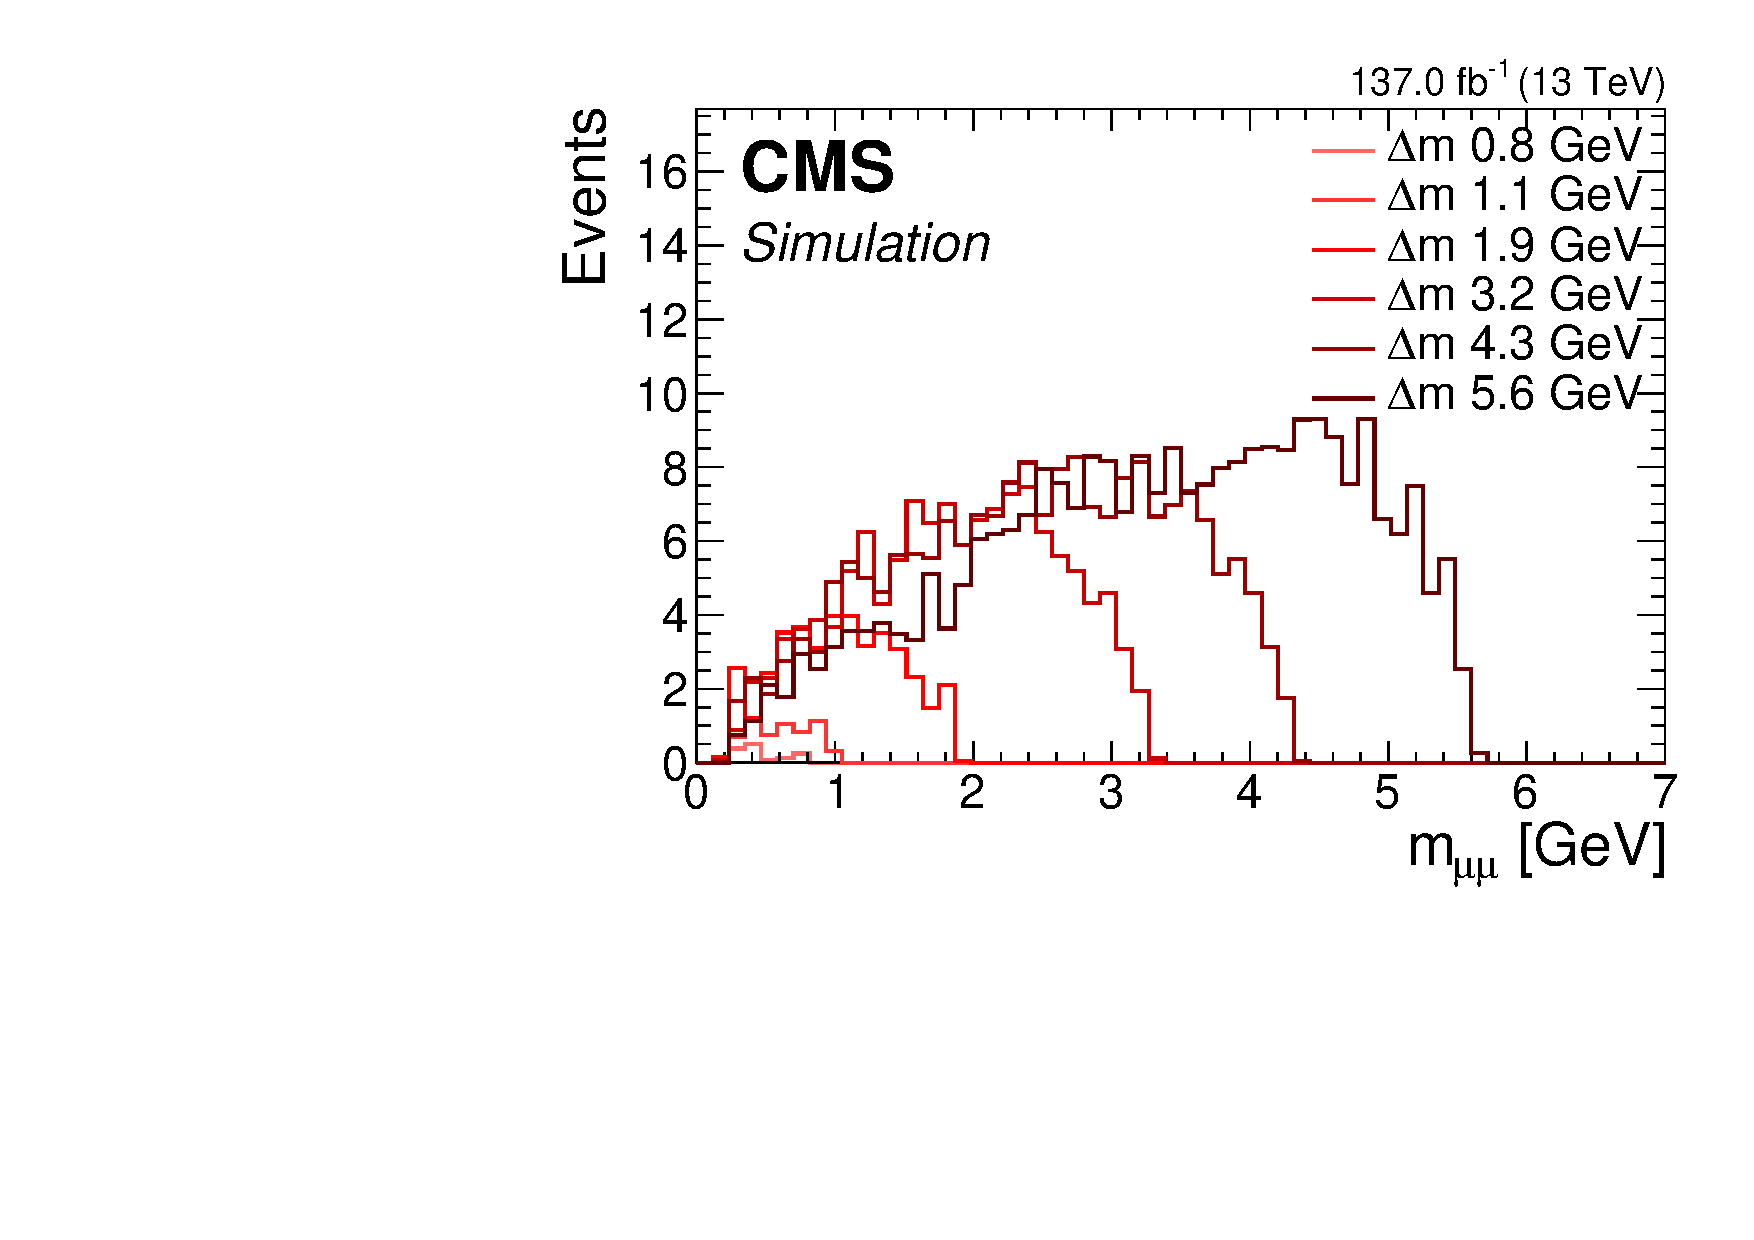
\includegraphics[width=0.48\linewidth]{plots/signal_muons/none_invMassCorrJetNoMultIso10Dr0.6.pdf} \,
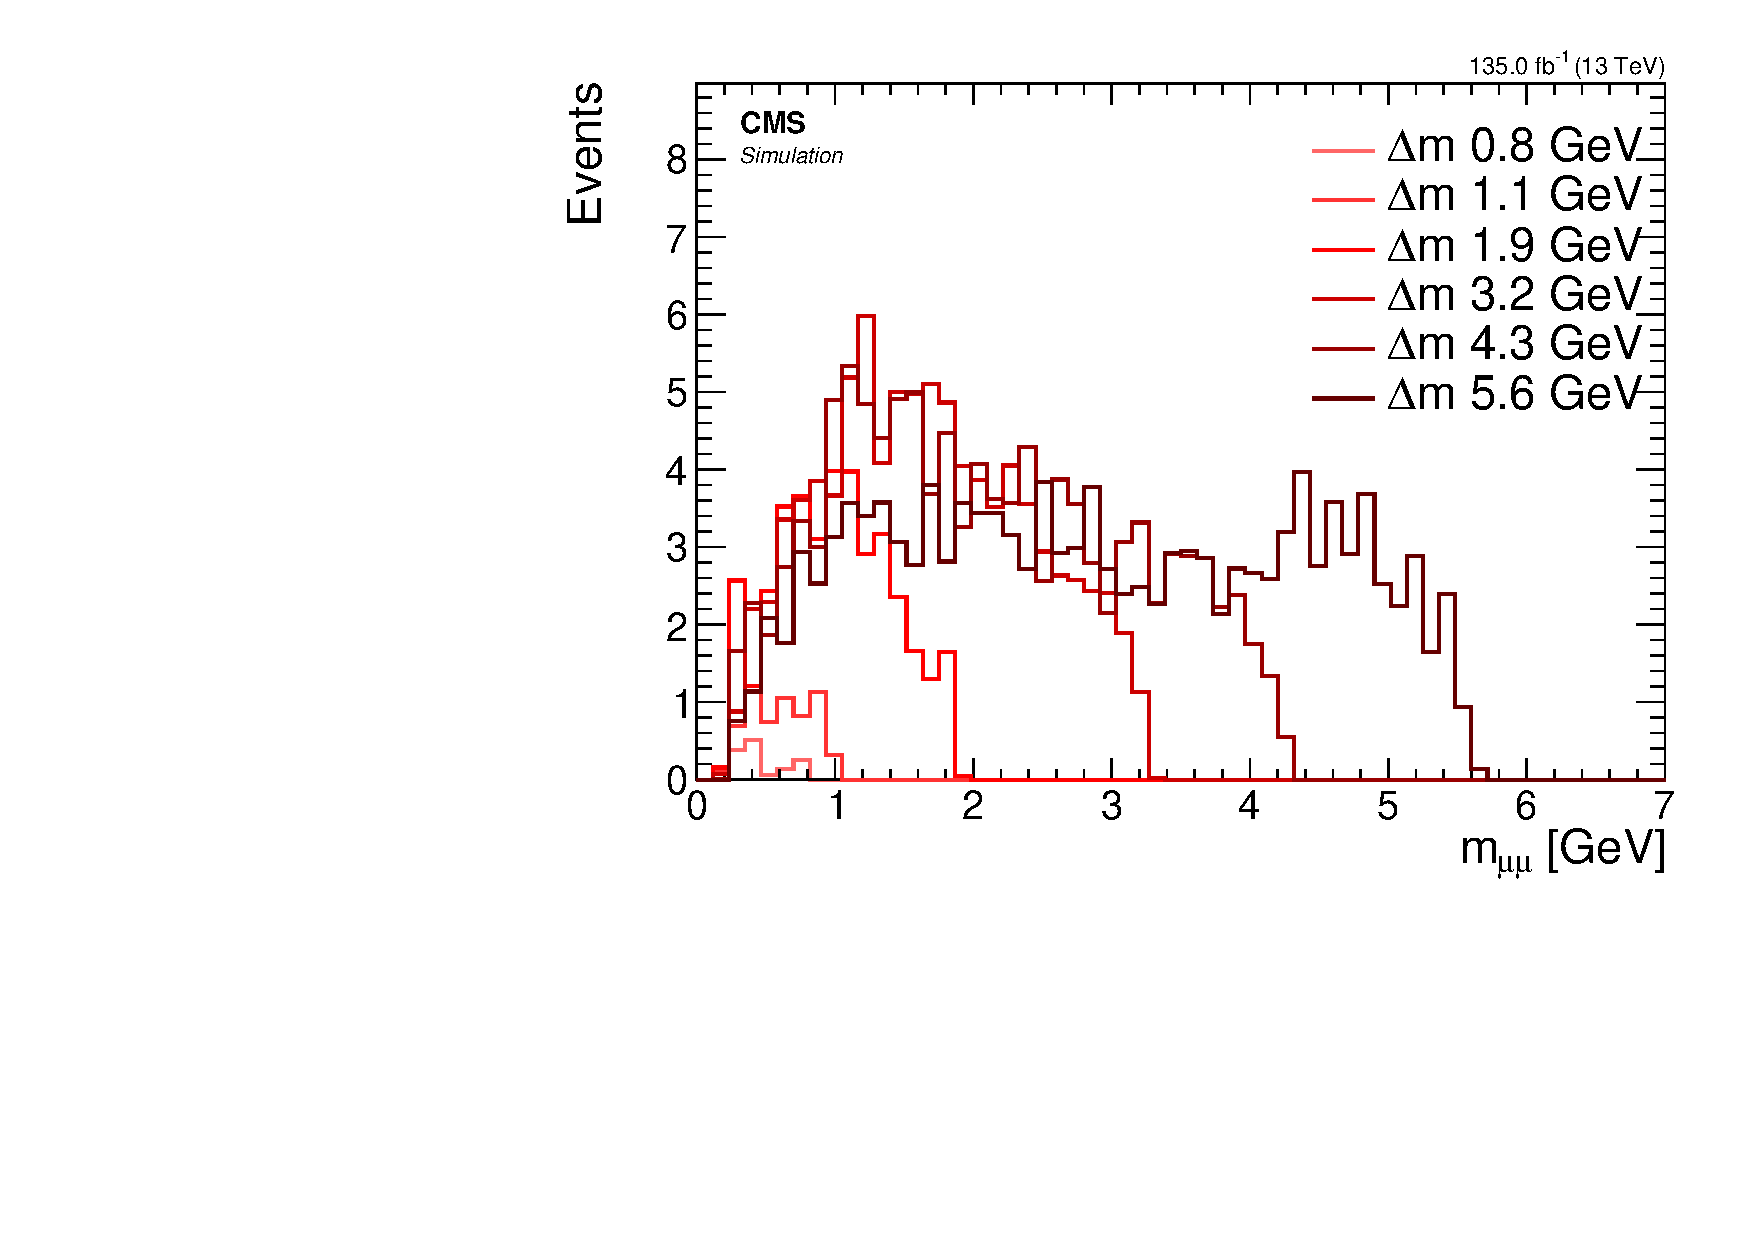
\includegraphics[width=0.48\linewidth]{plots/signal_muons/none_invMassCorrJetNoMultIso10Dr0.6_orth.pdf}  \\
\caption[Signal reconstructed \mmumu]{ Signal reconstructed \mmumu with basic analysis selection (left) and additional \gls{sos} orthogonality condition (right).}
\label{fig:reco-signal-invamass}
\end{figure}

It is interesting to compare these distributions to the two right ones in the generator level version at Figure~\ref{fig:signal-generator-mll}. It can be seen that not only are fewer events surviving the reconstruction, but also some \dm model points are peaking between $1 \GeV$ to $2 \GeV$ with the \gls{sos} orthogonality condition applied.

\subsubsection{Lepton separation \gls{dr}}
\label{sec:lepton-dr}

The lepton separation is defined by the equation $\DR=\sqrt{\left(\deta\right)^2+\left(\dphi\right)^2}$, where \gls{eta} represents the pseudorapidity and \gls{phi} is the azimuthal angle measured in radians. The value of \gls{dr} is significant in this analysis because the produced leptons tend to be located in proximity to each other and therefore are not easily isolated according to standard definitions. Special attention is given to ensuring that the collimated nature of the leptons can be used to differentiate the isolated leptons in the signal from the non-isolated leptons in the \gls{sm} background. It is worth noting that, for the purposes of orthogonality, we attempt to revert the requirement of $\drll > 0.3$ utilized in previous \gls{sos} analyses~\citep{sos}.

Similar to the invariant mass discussed in Section~\ref{sec:gen-invariant-mass}, we examine the distributions of \gls{dr} for various \dm options with different cuts applied to observe their effect.

\begin{figure}[!htb]
\centering
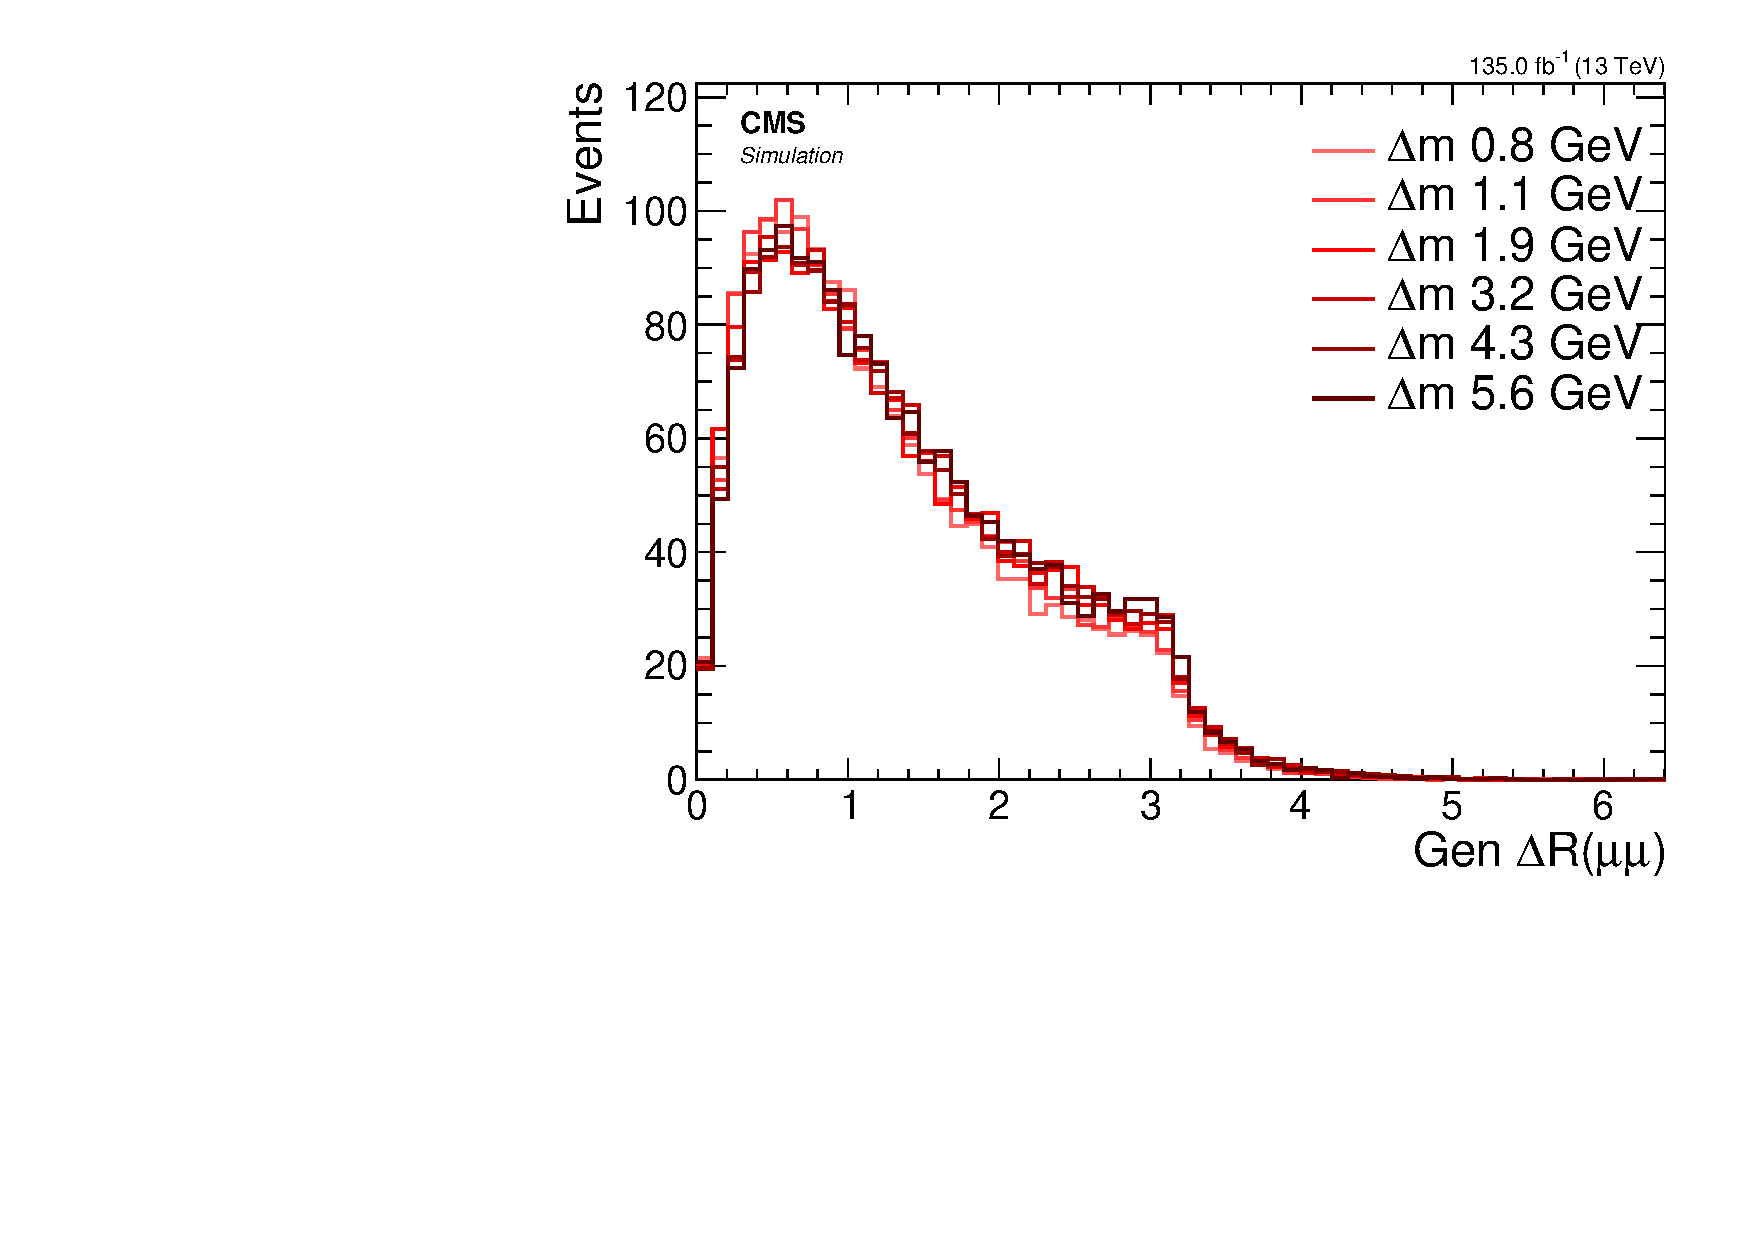
\includegraphics[width=0.32\linewidth]{plots/signal_muons_gen/none_gen_deltaR.pdf} \,
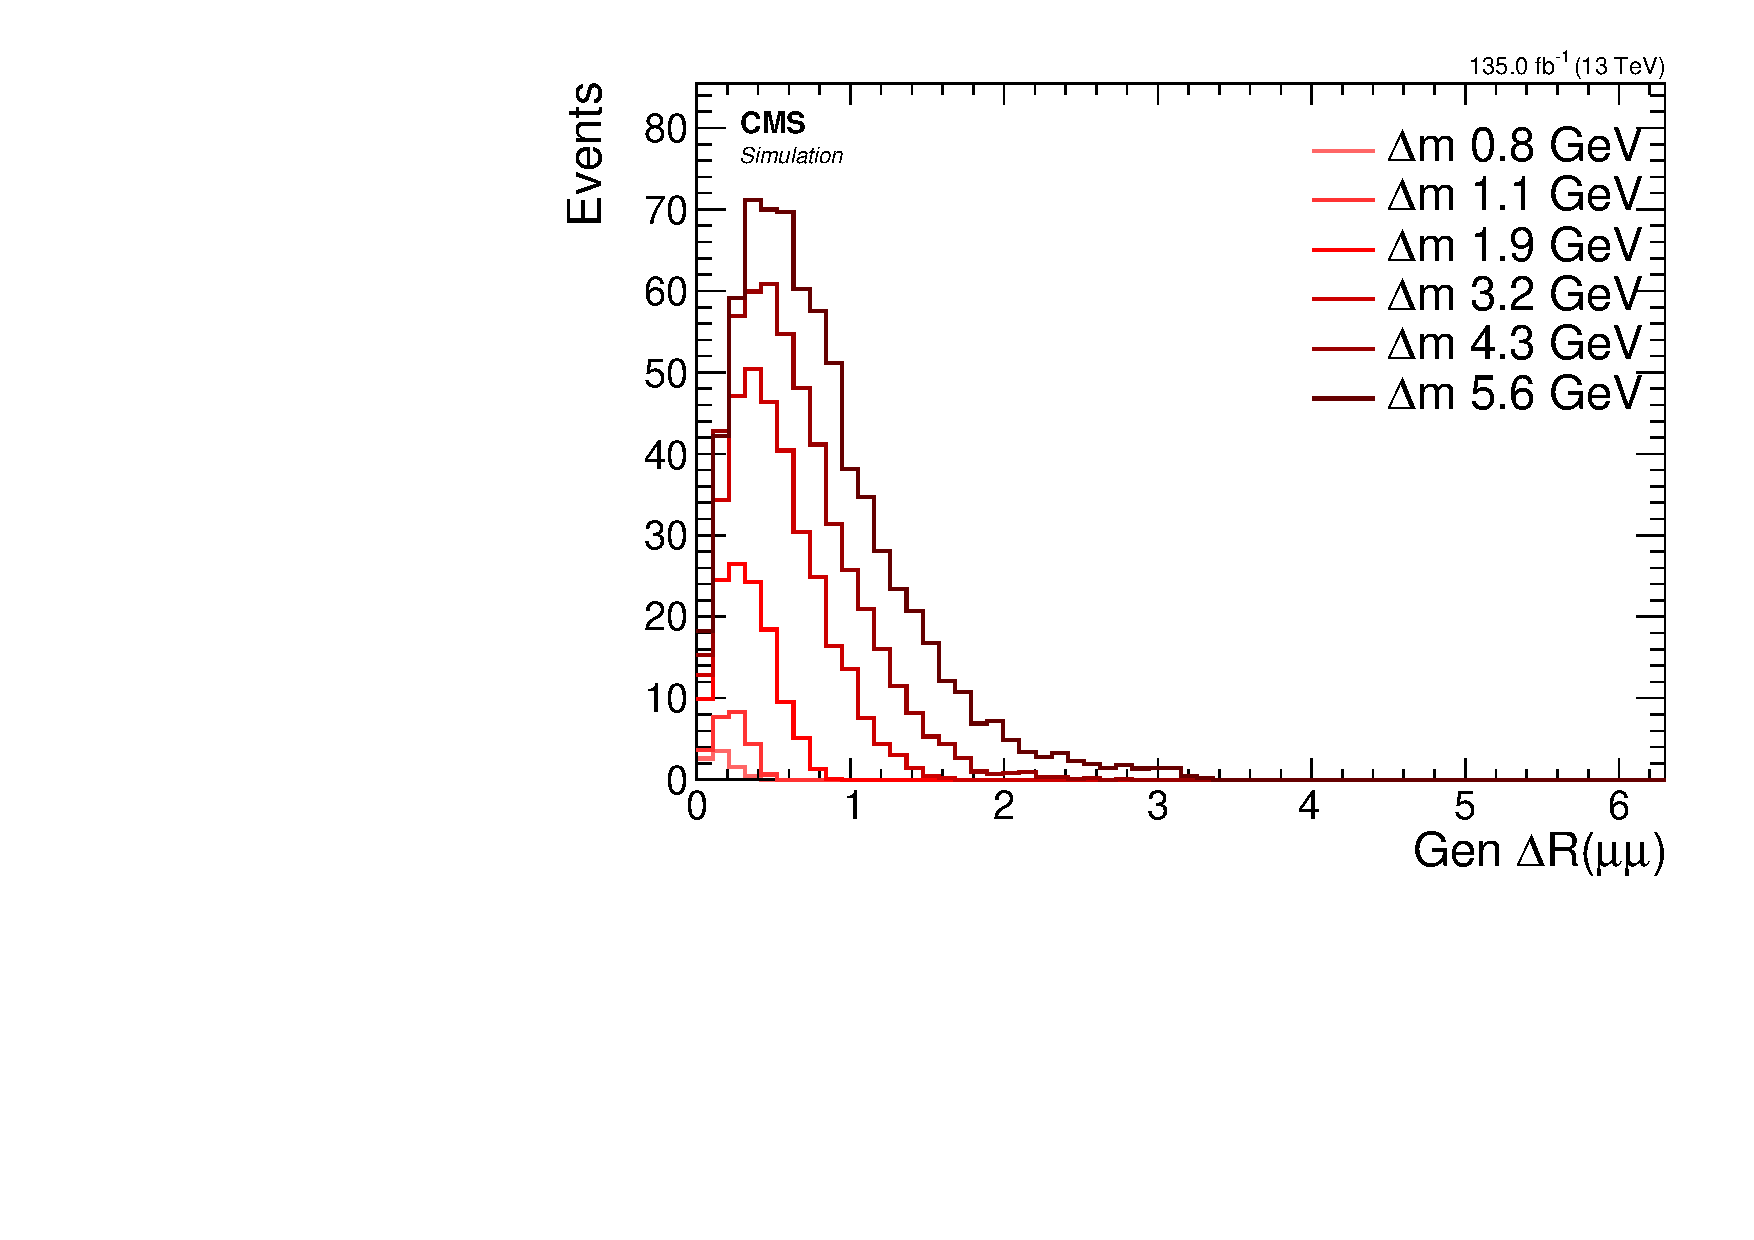
\includegraphics[width=0.32\linewidth]{plots/signal_muons_gen/none_gen_deltaR_cut.pdf}  \,
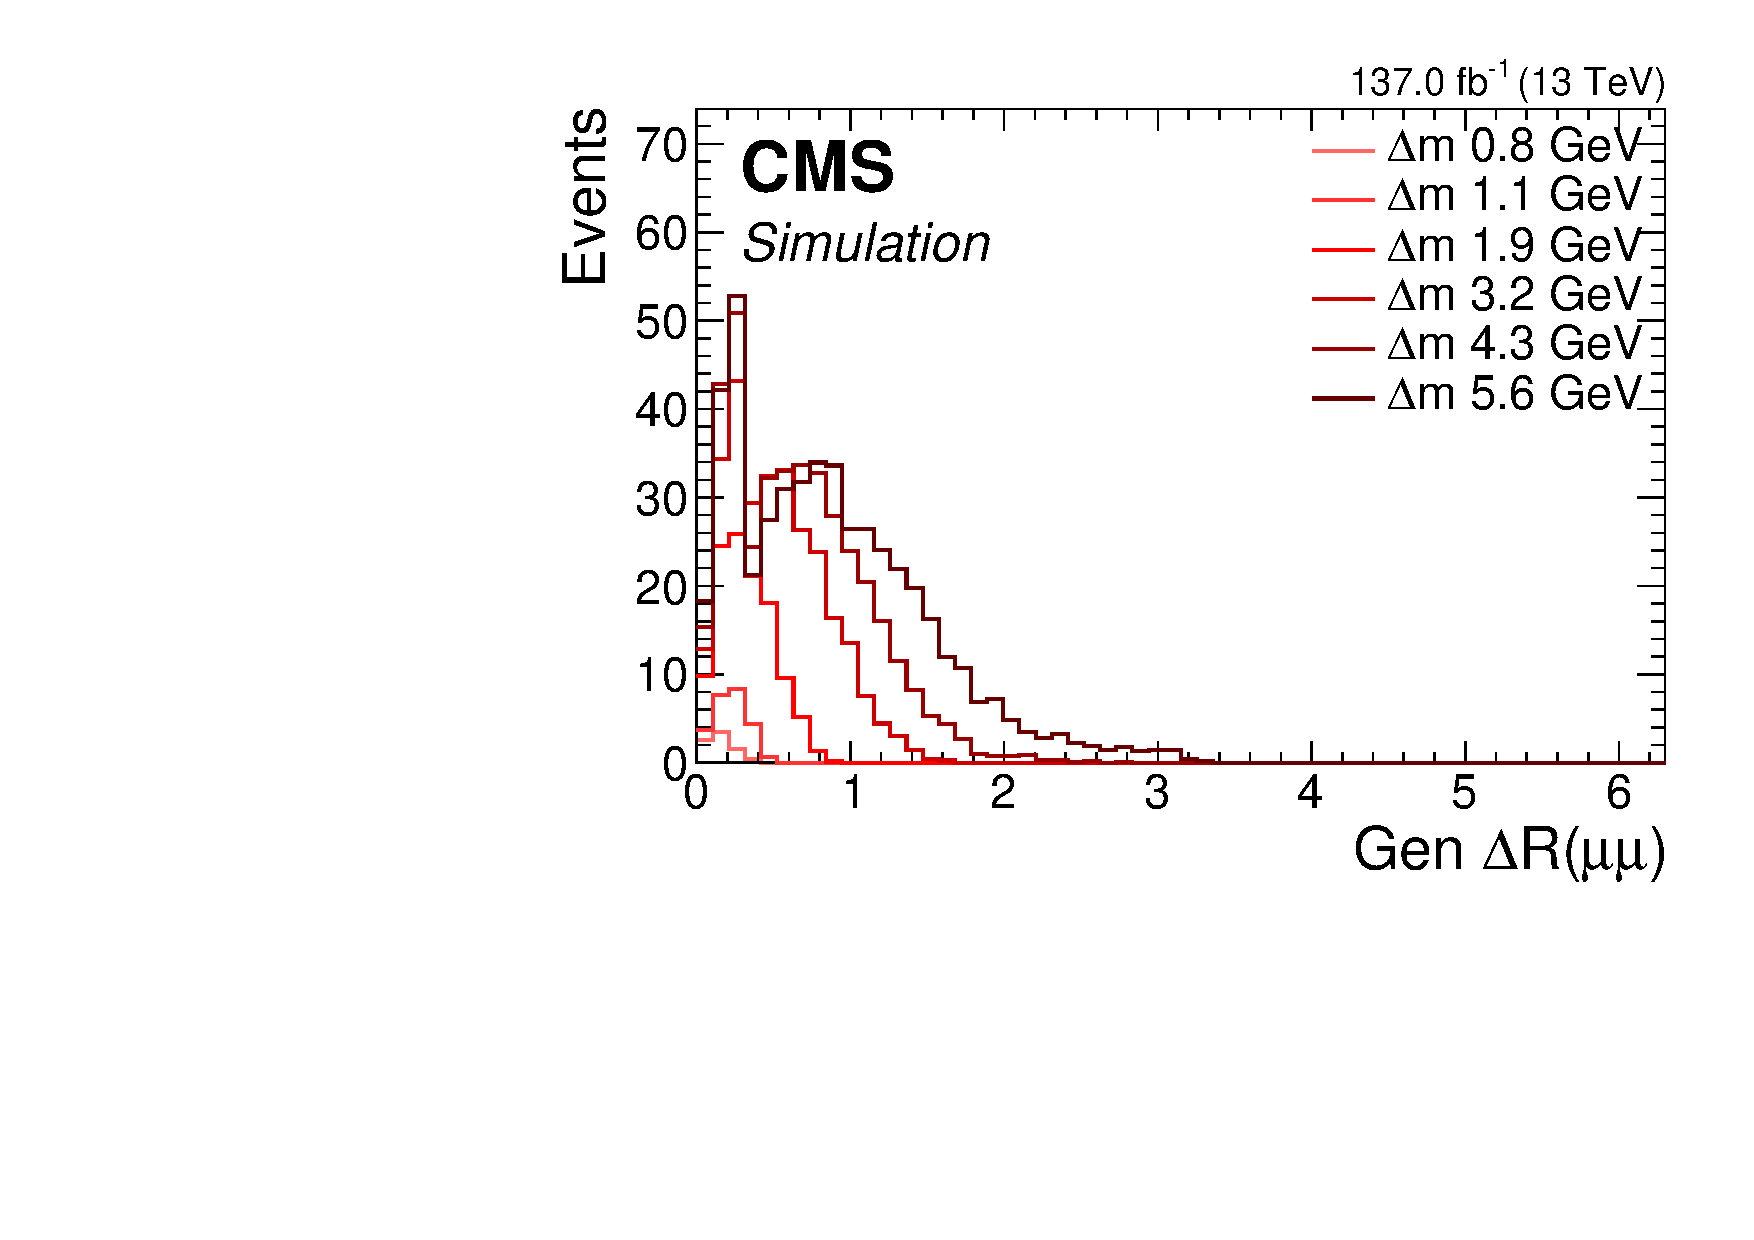
\includegraphics[width=0.32\linewidth]{plots/signal_muons_gen/none_gen_deltaR_orth.pdf} \\
\caption[Signal generator level \DR distributions]{ Signal generator level \gls{dr} distributions with no cuts (left), with $\pt\left(\mu_i\right)>2\GeV,\,i=1,2$ (middle) and with \gls{sos} orthogonality condition $\pt\left(\mu_i\right)>2\GeV$, $\pt\left(\mu_2\right)\leq~3.5\GeV\text{ or }\DR\leq 0.3$ (right).}
\label{fig:signal-generator-dr}
\end{figure}

The left plot of Figure~\ref{fig:signal-generator-dr} shows that roughly the same number of events are produced for all \dm model points. However, when applying a cut of $\pt\left(\mu\right)>2\GeV$, a hierarchy of \dm points emerges, with fewer events as \dm becomes smaller (middle plot). The spike on the right plot is due to the \gls{sos} orthogonality condition, which requires $\drll\leq 0.3$ as one of two conditions in an or statement.

To understand the shaping and hierarchy formation due to the \gls{pt} cut, the \pt of the muons is plotted \vs \drll, as shown in Figure~\ref{fig:signal-gen-dr-pt}.

\begin{figure}[!htb]
\centering
\includegraphics[width=0.48\linewidth]{plots/signal_muons_gen_delta_r_vs_pt/none_gen_delta_r_vs_pt_1.pdf} \,
\includegraphics[width=0.48\linewidth]{plots/signal_muons_gen_delta_r_vs_pt/none_gen_delta_r_vs_pt_2.pdf}  \\
\includegraphics[width=0.48\linewidth]{plots/signal_muons_gen_delta_r_vs_pt_dm5/none_gen_delta_r_vs_pt_1.pdf} \,
\includegraphics[width=0.48\linewidth]{plots/signal_muons_gen_delta_r_vs_pt_dm5/none_gen_delta_r_vs_pt_2.pdf}  \\
\caption[Signal \drmm \vs \pt]{ Signal \drmm \vs \pt for leading lepton $\mu_1$ (left) and subleading lepton $\mu_2$ (right) for $\dm=1.13\GeV$ (top) and $\dm=5.63\GeV$ (bottom).}
\label{fig:signal-gen-dr-pt}
\end{figure}

The hierarchy can be understood by observing that cutting on $\pt\left(\mu_2\right)\geq 2\GeV$ for $\dm=1.13\GeV$ will limit the range of \drmm to less than $0.4$, while leaving a large range exceeding 3 for the $\dm=5.63\GeV$ model point. It can be concluded that in order to gain access and sensitivity to the low \dm model points, probing low \drll values, potentially with values less than 0.3, is necessary, even before considering the reconstruction efficiency of the leptons. In the next sections, the study of reconstructed leptons and the definition of isolation criteria will enable the retention of signal points with close lepton pairs, as further explored in Section~\ref{sec:isolation}.

As seen in Section~\ref{sec:gen-invariant-mass} for \mmumu, reconstruction has an effect on both the shape and overall count of events. The effects on the \drmm distributions are investigated in Figure~\ref{fig:reco-signal-dr}.

\begin{figure}[!htb]
\centering
\includegraphics[width=0.48\linewidth]{plots/signal_muons/none_deltaRCorrJetNoMultIso10Dr0.6.pdf} \,
\includegraphics[width=0.48\linewidth]{plots/signal_muons/none_deltaRCorrJetNoMultIso10Dr0.6_orth.pdf}  \\
\caption[Signal reconstructed \drmm]{ Signal reconstructed \drmm with basic analysis selection (left) and additional \gls{sos} orthogonality condition (right).}
\label{fig:reco-signal-dr}
\end{figure}

When the reconstructed \drmm distributions in Figure~\ref{fig:reco-signal-dr} are compared to the generator level ones in Figure~\ref{fig:signal-generator-dr}, it can be observed that the main effect of the reconstruction on the \drmm is the overall normalization, which is due to reconstruction efficiency.

\clearpage 
\subsection{Main drivers of sensitivity}

Conclusions can be drawn from this signal distribution studies in regards to the main drivers to the sensitivity of different model points of this analysis, as well as of future analysis that might try to expend on this one. This section does not consider \gls{sm} background at all, making it hard to conclude what effects changing the cuts to \MET or other event level observables might have. However, one thing is very clear from examining the dilepton kinematics, and that is to gain access to low \dm model points, the threshold on the \pt of the decay leptons must be lowered and low \gls{dr} must be probed. Another driver of the sensitivity at all \dm model points is the luminosity, since the production cross section drops as a function of the higgsino mass parameter $\mu$.

The next sections will explore how to lower the threshold on the muons transverse momentum and deal with collimated leptons that might pose a challenge in regards to the isolation criterion.


\section{Simulated samples}
\subsection{Standard Model simulated samples}
\label{sec:sm-mc}
\subsection{Signal simulated samples}
\label{sec:signal-simulation}

%don't capitalise 
\section{Object definition and selection}
\subsection{Electrons}
\subsubsection{Signal electron selection}
\subsubsection{Additional electron veto}
\subsection{Muons}
\subsubsection{Signal muon selection}
\label{sec:muon-selection}
\subsubsection{Additional muon veto}

\clearpage
\section{Trigger}
\label{sec:trigger}

Events in the \gls{sr}, as well as events in all \glspl{cr}, were collected using a set of triggers based on missing transverse energy \MET (or {\tt MET}) and missing hadronic transverse momentum \mht (or {\tt MHT}), denoted by the HLT paths 
%a set of \ptmiss- and \hardmet-based triggers, denoted by the HLT paths

\begin{itemize}
\item
  \texttt{HLT\_PFMETX\_PFMHTX\_IDTight\_v* (X=90,100,110,120,130,140)} and
\item \texttt{HLT\_PFMETNoMuX\_PFMHTNoMuX\_IDTight\_v* (X=90,100,110,120,130,140)}.
\end{itemize}

Here, \texttt{X} indicates the threshold applied to the online \MET and \mht, as calculated by the \gls{pf} algorithm; the asterisks indicate that more than one version of the same trigger may have been used. During periods of higher instantaneous luminosity, trigger paths with lower thresholds became prescaled to reduce the
event rate; in such cases, the search relies on the higher-threshold triggers, which remained un-prescaled throughout all data-taking periods. To compensate for losses in efficiency associated with the higher trigger thresholds,  
a set of back-up triggers was used when the  low-threshold \MET-\mht triggers became prescaled:

\begin{itemize}
\item \texttt{HLT\_PFMETX\_PFMHTX\_IDTight\_PFHT60\_v* (X=100,110,120,130,140)},
\item \texttt{HLT\_PFMETNoMuX\_PFMHTNoMuX\_IDTight\_PFHT60\_v* (X=100,110,120,130,140)},
\item \texttt{HLT\_PFMET120\_PFMHT120\_IDTight\_HFCleaned\_v*},
\item \texttt{HLT\_PFMET120\_PFMHT120\_IDTight\_PFHT60\_HFCleaned\_v*}, and
\item \texttt{HLT\_PFMETNoMu120\_PFMHTNoMu120\_IDTight\_HFCleaned\_v*}.
\end{itemize}

The logical OR of all of the above trigger paths was taken as the online criterion for selecting events throughout the three years of
data-taking.  The efficiency of the trigger decision is estimated in a single-electron CR collected the single-electron trigger path
\begin{itemize}
\item \texttt{HLT\_Ele27\_WPTight\_Gsf\_v*}.
\end{itemize}
The efficiency is estimated as
\begin{equation}
\epsilon = \frac{ n_{\text{ev}}(\text{passing \MET-\mht trigger in reference sample}) }{n_{\text{ev}}(\text{reference sample})},
\end{equation}
where the reference sample corresponds to events passing the electron trigger and additionally required to have an offline electron with $\pt>30$ GeV and $|\eta|<2.4$ passing the Medium WP. The efficiency is shown as a function of offline analysis observables \mht and \njets in Figure~\ref{fig:main-trigger-real-met}.

\begin{figure}[]
\centering
\includegraphics[width=0.48\linewidth]{plots/trigger/TrigEffMht.pdf}
\includegraphics[width=0.48\linewidth]{plots/trigger/TrigEffNJets.pdf}
\caption[The efficiency of the set of \MET-\mht cross triggers]{The efficiency of the set of \MET-\mht cross triggers measured in a single-electron control region, shown for \mht (left) and number of jets (right). The jet multiplicity is shown for \mht$>300$ GeV to account for the trigger turn-on.
  % This trigger set used to collect events in the signal region as well as the   single-lepton and QCD validation control  regions.
  %The measured efficiency is applied as an event weight to simulated signal events.
  }
\label{fig:main-trigger-real-met}
\end{figure}

The trigger efficiency has been studied previously, e.g., in SUS-19-006~\cite{CMS-PAS-SUS-19-006}, the efficiency measured in the SingleElectron datastream is consistent with the efficiency corresponding to SUSY signal events. The efficiency is applied as event weights extracted from the binned efficiency shown in Figure~\ref{fig:main-trigger-real-met}.





\clearpage
\section{Event selection}
\label{sec:event-selection}

As discussed in Section~\ref{sec:search-strategy}, three event categories are used in this analysis: the dimuon category and an exclusive track category for each lepton flavor (muon and electron). The preselection is summarized in Section~\ref{sec:preselection}, followed by the selection that defines each category in Section~\ref{sec:category-selection}. Finally, the multivariate selection for each category is discussed in Section~\ref{sec:event-bdt}.

\subsection{Preselection}
\label{sec:preselection}

In Section~\ref{tab:base-selection}, the preselection criteria that apply to all categories was defined. This section reiterates the reasons for this selection as well as describes other event-level selections.

\begin{itemize}

\item $\mht\geq220\GeV$ and $\MET \geq 140\GeV$ cuts are intended to boost sensitivity by rejecting \gls{sm} background and to operate in the acceptance regime of the MET trigger, as described in Section~\ref{sec:trigger}. These cuts are especially efficient in rejecting \gls{qcd} background, which does not produce real \MET. Any \MET apparent in \gls{qcd} is due to jet energy miss-measurements. The harder cut on \mht is made instead of \MET because \mht sums jets with $\pt>30\GeV$ and is blind to objects with $\pt<30\GeV$. Background estimation relies on jets with \pt in the range of $[15,30]\GeV$, so \mht avoids introducing bias in the data-driven background estimation methods.

\item $\njets \left( \pt \geq 30\GeV\, \mathrm{and}\, \abs{\eta} < 2.4 \right) \geq 1$. At least one jet is required in the event because such an \gls{isr} jet gives a boost to the produced neutralino, thus increasing the missing transverse energy and the sensitivity of the analysis.

\item $\nbjets \left( \pt \geq 30\GeV\, \mathrm{and}\, \abs{\eta} < 2.4 \right) = 0$. Any event with medium WP \PQb-tagged jet is vetoed since our signal does not contain real \PQb-tagged jets. This veto is efficient in rejecting background from \ttbar, in which the \PQb quarks arise from a \PQt quark decay.

\item $\mindphimhtjets$  $ > 0.4$. Requiring an \gls{isr} jet in the event leads to the expectation that the $\mht$ should point in the opposite direction of the jet at an angle close to $\pi$. In QCD events, fake \mht can arise from jet with much too low reconstructed \pt, which are vetoed by this cut.

\item veto events with isolated loose-ID lepton having $\pt\geq 30\GeV$. Lepton can be either muon or electron. This reduces $\PW\rightarrow\ell\PGn$ decays.

\item $0.4<\mll<12 \GeV$. The signal resides in an invariant mass window with an edge at the mass difference between \neutt and \neuto. This is a relatively loose cut that is expected to be further tightened by the boosted decision tree.

\end{itemize}

The object level selection for electrons and muons was described in detail in Section~\ref{sec:object-selection}. 

\subsection{Category selection}
\label{sec:category-selection}

The selection criteria for the dilepton category are described in Section~\ref{sec:dilepton-selection}, while those for the exclusive track category are detailed in Section~\ref{sec:exclusive-track-selection}.

\subsubsection{Dilepton selection}
\label{sec:dilepton-selection}

In the dilepton category, two reconstructed and identified muons are required. Events in the di-lepton category must satisfy the preselection and the baseline selection, as well as the following criteria:

\begin{itemize}

\item $N_\mu = 2$ with opposite-charge satisfying the analysis muon selection;
\item $\pt(\mu_2)\leq 3.5\GeV$ or $\DR(\mu_1,\mu_2) < 0.3$. This requirement ensures the analysis is orthogonal, that is, non-overlapping in terms of event content, with the previously published soft lepton analysis~\cite{sos};
\item Event BDT score $\mathrm{BDT} > 0$. This is the main method of selecting signal events while rejecting the \gls{sm} background. Details are given in Section~\ref{sec:event-bdt};
\item $\DR(\mu_{1,2},j_1) > 0.4$, where $j_1$ is the leading jet. The leptons should not be inside the \gls{isr} jet;
\item \PGo, $\PGr^0$ and \JPsi invariant mass vetoes. $\mll \notin [0.75,0.81]\GeV,\,\mll \notin [3,3.2]\GeV$.
\end{itemize}

\subsubsection{Exclusive track selection}
\label{sec:exclusive-track-selection}

The exclusive track category requires one reconstructed and identified lepton, which can be either an electron or a muon, and an exclusive track, meaning a track that is not identified as a lepton. The track with the highest track \gls{bdt} score, as described in Section~\ref{sec:track-bdt}, is picked as the signal lepton candidate. Events in this category must satisfy the preselection and the baseline selection, as well as the following criteria:

\begin{itemize}

\item $N_\ell = 1$ lepton passing the analysis muon or electron selection;
\item maximum track picking BDT score $ > 0$, as discussed in~\ref{sec:track-bdt};
\item event level BDT score $ > 0$. This is the main method of selecting signal events while rejecting the \gls{sm} background, as discussed in Section~\ref{sec:event-bdt};
\item $\DR(\ell,j_1) > 0.4$, where $j_1$ is the highest-pT jet. The lepton should not be inside the \gls{isr} jet.
\end{itemize}

\subsection{Binary event classifier}
\label{sec:event-bdt}

This analysis employs a multivariate classifier to select signal events while optimally rejecting SM background events. The classifier algorithm is a \gls{bdt}, and its output score is used to define \glsreset{sr}\glspl{sr} as well as \glsreset{sr}\glspl{cr}. For the dimuon category, one \gls{bdt} is trained, while for the exclusive track category, a \gls{bdt} is trained for each lepton flavor and for the two phases of the tracker detector (Phase 0 and Phase 1), resulting in a total of five \glspl{bdt}.

All \glspl{bdt} are based on the same architecture, making use of 120 trees with a maximum depth of 3. The \gls{bdt} training is performed with AdaBoost and GiniIndex separation. The BDTs are trained and evaluated using the TMVA package~\cite{tmva}. 

For training, signal events are taken from the dedicated samples used to train the track-picking BDT for the exclusive track category, listed in Section~\ref{sec:signal-simulation}, and SM samples listed in Section~\ref{sec:sm-mc} for the background. For the exclusive track category, MC from 2016 and 2017 are used to represent Phase 0 and Phase 1 of the tracker, respectively. For the dimuon category, only 2017 MC is used to represent both phases, with an added systematic uncertainty resulting from this choice.

For the signal the same broad range of higgsino parameter $\mu$ (\PSGcpmDo) is used as was considered for the track-picking BDT training sample, but only the range of \dm targeted by the analysis. For Phase 0, $\dmo$ is selected in the range of [0.3, 4.3]\GeV and $\mu$ is selected in the range [100,130]\GeV. For Phase 1, $\dmpm$ is selected in the range of [0.3-4.6]\GeV and $\mu$ is selected in the range of [100-500]\GeV. The preselection and baseline selection is applied to the events included in the training, as well as a subset of the selection criteria listed in Section~\ref{sec:dilepton-selection} and Section~\ref{sec:exclusive-track-selection} in order to increase MC statistics. It is as follows:

\begin{itemize}

\item $N_\mu = 2 (1)$ opposite-charge passing the muon selection for the dimuon category (for the exlusive track category);

\item $\DR(\ell),\text{leading jet}) > 0.4$;

\item track picking BDT score $ > 0$ for the exclusive track category.

\end{itemize}

The training was conducted without using \gls{mc} weights to avoid possible overtraining issues. This choice does not compromise the performance of the BDT because the kinematics of low-\pt leptons are similar across most \gls{sm} background production processes. When examining the distributions of input variables in the following sections, this fact must be taken into account. The distributions are plotted without \gls{mc} weights and with signal events taken from a pool of different parameter values as described above. Therefore, the ROC curves cannot be understood as a simple signal efficiency versus background rejection. Each \gls{bdt} output working point results in a different signal efficiency depending on the signal parameter values. As will be seen later, one does not use a single value of \gls{bdt} with a simple cut and count. Instead, the \glspl{sr} are binned according to \gls{bdt} output values. Therefore, the ROC curve is plotted with a default cut of 0.0 on the BDT output. To fully estimate the power of the training, one needs to consider the significance when each signal point has been properly weighted together with the background processes from the \gls{sm}.

\subsubsection{Dimuon category}

The training samples for the dimuon category contain 4350 signal events and 21842 background events. The \gls{bdt} is evaluated in statistically independent samples of the same size in order to identify any overtraining. The distributions of the testing samples superimposed on the training samples, as well as the ROC curve, are shown in Figure~\ref{fig:event-bdt-dimuon-output}. No significant overtraining is observed. The BDT takes 18 variables as input, listed in Table~\ref{tab:dimuon-bdt-variables} in decreasing order of importance ranking.

\begin{figure}[!htb]
\centering
\includegraphics[width=0.48\linewidth]{plots/dimuon_bdt/overtraining_Event_Dilepton_Muons_Phase_1.pdf} \,
\includegraphics[width=0.48\linewidth]{plots/dimuon_bdt/roc_Event_Dilepton_Muons_Phase_1.pdf} \\


\caption[Dimuon BDT output and ROC curve]{Dimuon BDT output (left) and ROC curve (right).}
\label{fig:event-bdt-dimuon-output}
\end{figure}

\begin{table}[!htb]
	\centering
	
		\caption{\label{tab:dimuon-bdt-variables}Dimuon BDT input variables ranked in order of importance, as reported in the TMVA performance summary table.}
		%\vspace{1mm}
			\begin{tabular}{cll} \hline
			Rank & Variable & Description \\ \hline
			1 & $\mll$ & invariant mass \\
			2 & $\pt(\ell_1)$ & leading lepton \pt\\
			3 & \mht & \\
			4 & \HT & \\
			5 & $\DR\left(\ell\ell\right)$ & \\
			6 & $\mindphimhtjets$ & \\
			7 & $\pt(\vec{\ell}_1+\vec{\ell}_2)$ & dilepton \pt \\
			
			8 & $\pt(\text{leading jet})$ & \\		
			9 & $\pt(\ell_2)$ & subleading lepton \pt \\
			10 & $\eta(\ell_1)$ & leading lepton $\eta$ \\
			11 & $m_T(\ell_1)$ & leading lepton transverse mass\\
			
			12 & $\abs{\Delta\phi\left(\ell_2, \htvecmiss \right)}$ & \\
			13 & $\abs{\Delta\phi\left(\ell_1, \htvecmiss \right)}$ & \\			
			14 & $\abs{\Delta\phi\left(\ell\ell \right)}$ & \\			
			15 & $\njets$ & Number of jets \\ 
			16 & $\eta(\text{leading jet})$ & \\
			17 & $\abs{\Delta \eta \left(\ell \ell\right) }$ & \\
			18 & $\mtautau$ & collinear approximation of $\mtautau$\\
			\hline
			\end{tabular}
\end{table}

Distributions of the input variables to the \gls{bdt} are shown in Figure~\ref{fig:dimuon-input-distributions}.

\begin{figure}[!htb]
\centering
\includegraphics[width=0.32\linewidth]{plots/dilepton_bdt_inputs_muons/none_invMassCorrJetNoMultIso10Dr0.6.pdf} \,
\includegraphics[width=0.32\linewidth]{plots/dilepton_bdt_inputs_muons/none_leptonsCorrJetNoMultIso10Dr0.6_0_.Pt__.pdf} \,
\includegraphics[width=0.32\linewidth]{plots/dilepton_bdt_inputs_muons/none_MHT.pdf}   \\
\includegraphics[width=0.32\linewidth]{plots/dilepton_bdt_inputs_muons/none_HT.pdf} \,
\includegraphics[width=0.32\linewidth]{plots/dilepton_bdt_inputs_muons/none_deltaRCorrJetNoMultIso10Dr0.6.pdf}  \,
\includegraphics[width=0.32\linewidth]{plots/dilepton_bdt_inputs_muons/none_MinDeltaPhiMhtJets.pdf} \\


\includegraphics[width=0.32\linewidth]{plots/dilepton_bdt_inputs_muons/none_dileptonPtCorrJetNoMultIso10Dr0.6.pdf} \,
\includegraphics[width=0.32\linewidth]{plots/dilepton_bdt_inputs_muons/none_LeadingJetPt.pdf} \,
\includegraphics[width=0.32\linewidth]{plots/dilepton_bdt_inputs_muons/none_leptonsCorrJetNoMultIso10Dr0.6_1_.Pt__.pdf}   \\
\includegraphics[width=0.32\linewidth]{plots/dilepton_bdt_inputs_muons/none_leptonsCorrJetNoMultIso10Dr0.6_0_.Eta__.pdf} \,
\includegraphics[width=0.32\linewidth]{plots/dilepton_bdt_inputs_muons/none_mth1CorrJetNoMultIso10Dr0.6.pdf}  \,
\includegraphics[width=0.32\linewidth]{plots/dilepton_bdt_inputs_muons/none_deltaPhiMhtLepton2CorrJetNoMultIso10Dr0.6.pdf} \\


\includegraphics[width=0.32\linewidth]{plots/dilepton_bdt_inputs_muons/none_deltaPhiMhtLepton1CorrJetNoMultIso10Dr0.6.pdf} \,
\includegraphics[width=0.32\linewidth]{plots/dilepton_bdt_inputs_muons/none_deltaPhiCorrJetNoMultIso10Dr0.6.pdf} \,
\includegraphics[width=0.32\linewidth]{plots/dilepton_bdt_inputs_muons/none_NJets.pdf}   \\
\includegraphics[width=0.32\linewidth]{plots/dilepton_bdt_inputs_muons/none_LeadingJet.Eta__.pdf} \,
\includegraphics[width=0.32\linewidth]{plots/dilepton_bdt_inputs_muons/none_deltaEtaCorrJetNoMultIso10Dr0.6.pdf}  \,
\includegraphics[width=0.32\linewidth]{plots/dilepton_bdt_inputs_muons/none_nmtautauCorrJetNoMultIso10Dr0.6_log.pdf} \\

\caption[dimuon training input distribution]{Dimuon BDT training input variables. The plots are ordered by importance ranking.}
\label{fig:dimuon-input-distributions}
\end{figure}

\clearpage
\subsubsection{Exclusive track category}

The training samples for Phase 0 for the exclusive  category contain 7863 (1750) signal events and 55765 (29135) background events for muons (electrons). For Phase 1, the exclusive category contains 5266 (1332) signal events and 51308 (31149) background events for muons (electrons). The distributions of the exclusive track category BDT output of the testing samples superimposed on the training samples are shown in Figure~\ref{fig:event-bdt-ex-track-output}. The ROC curves are seen in Figure~\ref{fig:event-bdt-ex-track-roc}. No overtraining is observed.

\begin{figure}[!htb]
\centering
\includegraphics[width=0.48\linewidth]{plots/extrack_bdt/overtraining_Event_Ex_Track_Muons_Phase_0.pdf} \,
\includegraphics[width=0.48\linewidth]{plots/extrack_bdt/overtraining_Event_Ex_Track_Electrons_Phase_0.pdf} \\

\includegraphics[width=0.48\linewidth]{plots/extrack_bdt/overtraining_Event_Ex_Track_Muons_Phase_1.pdf} \,
\includegraphics[width=0.48\linewidth]{plots/extrack_bdt/overtraining_Event_Ex_Track_Electrons_Phase_1.pdf} \\

\caption[Exclusive track category BDT outputs]{Exclusive track category BDT output in Phase 0 (top) and Phase 1 (bottom) for muons (left) and electrons (right).}
\label{fig:event-bdt-ex-track-output}
\end{figure}

\begin{figure}[!htb]
\centering
\includegraphics[width=0.48\linewidth]{plots/extrack_bdt/roc_Event_Ex_Track_Muons_Phase_0.pdf} \,
\includegraphics[width=0.48\linewidth]{plots/extrack_bdt/roc_Event_Ex_Track_Electrons_Phase_0.pdf} \\

\includegraphics[width=0.48\linewidth]{plots/extrack_bdt/roc_Event_Ex_Track_Muons_Phase_1.pdf} \,
\includegraphics[width=0.48\linewidth]{plots/extrack_bdt/roc_Event_Ex_Track_Electrons_Phase_1.pdf} \\

\caption[Exclusive track category ROC curve]{Exclusive track category ROC curves in Phase 0 (top) and Phase 1 (bottom) for muons (left) and electrons (right)}
\label{fig:event-bdt-ex-track-roc}
\end{figure}

The training uses 18 different variables listed in Table~\ref{tab:extrack-bdt-variables} in decreasing order of importance ranking. Since the ranking is slightly different in the four trainings, the order in the case of the muons of phase 1 is chosen to be listed here. The identified lepton is denoted as $\ell$ and the non-identified lepton track as $t$.

\begin{table}[!htb]
	\centering
	
		\caption{\label{tab:extrack-bdt-variables}Exclusive track BDT input variables}
		%\vspace{1mm}
			\begin{tabular}{cll} \hline
			Rank & Variable & Description \\ \hline
			1 & $\pt(\ell)$ & lepton \pt\\
			2 & \HT & \\
			3 & \mht & \\
			4 & $\mindphimhtjets$ & \\
			5 & $\pt(\text{leading jet})$ & \\
			6 & $\njets$ & Number of jets \\					7 & track BDT output & \\
			8 & $\eta(t)$ & \\
			9 & $\pt(t)$ & track \pt\\
			10 & $\eta(\text{leading jet})$ & \\				11 & $\mll$ & invariant mass \\
			12 & $\eta(\ell)$ & \\
			13 & $m_T(\ell)$ & lepton transverse mass\\			
			14 & $\DR\left(\ell, t\right)$ & \\
			15 & $\phi(\ell)$ & \\
			16 & $\phi(t)$ & \\
			17 & $\abs{\Delta\phi\left(\ell,t \right)}$ & \\			
			18 & $\abs{\Delta \eta \left(\ell, t\right) }$ & \\			
			\hline
			\end{tabular}
\end{table}

Distributions of the input variables to the \gls{bdt} training can be seen in Figure~\ref{fig:extrack-input-distributions}. As mentioned before, the signal is taken from a pool of a range of model points, and events are not weighted to any luminosity or cross section in order to avoid overtraining. In the following sections the fully weighted distributions will be shown in order to asses the performance of the training for different model points and to understand the different components of the standard model background and how to estimate them properly.

\begin{figure}[!htb]
\centering
\includegraphics[width=0.32\linewidth]{plots/extrack_bdt_inputs_muons/none_MinDeltaPhiMhtJets.pdf} \,
\includegraphics[width=0.32\linewidth]{plots/extrack_bdt_inputs_muons/none_leptonCorrJetNoMultIso10Dr0.6.Pt__.pdf} \,
\includegraphics[width=0.32\linewidth]{plots/extrack_bdt_inputs_muons/none_NJets.pdf}   \\
\includegraphics[width=0.32\linewidth]{plots/extrack_bdt_inputs_muons/none_HT.pdf} \,
\includegraphics[width=0.32\linewidth]{plots/extrack_bdt_inputs_muons/none_MHT.pdf}  \,
\includegraphics[width=0.32\linewidth]{plots/extrack_bdt_inputs_muons/none_exTrack_invMassCorrJetNoMultIso10Dr0.6.pdf} \\


\includegraphics[width=0.32\linewidth]{plots/extrack_bdt_inputs_muons/none_mtlCorrJetNoMultIso10Dr0.6.pdf} \,
\includegraphics[width=0.32\linewidth]{plots/extrack_bdt_inputs_muons/none_LeadingJetPt.pdf} \,
\includegraphics[width=0.32\linewidth]{plots/extrack_bdt_inputs_muons/none_leptonCorrJetNoMultIso10Dr0.6.Eta__.pdf}   \\
\includegraphics[width=0.32\linewidth]{plots/extrack_bdt_inputs_muons/none_trackBDTCorrJetNoMultIso10Dr0.6.pdf} \,
\includegraphics[width=0.32\linewidth]{plots/extrack_bdt_inputs_muons/none_trackCorrJetNoMultIso10Dr0.6.Eta__.pdf}  \,
\includegraphics[width=0.32\linewidth]{plots/extrack_bdt_inputs_muons/none_exTrack_deltaEtaCorrJetNoMultIso10Dr0.6.pdf} \\


\includegraphics[width=0.32\linewidth]{plots/extrack_bdt_inputs_muons/none_leptonCorrJetNoMultIso10Dr0.6.Phi__.pdf} \,
\includegraphics[width=0.32\linewidth]{plots/extrack_bdt_inputs_muons/none_trackCorrJetNoMultIso10Dr0.6.Phi__.pdf} \,
\includegraphics[width=0.32\linewidth]{plots/extrack_bdt_inputs_muons/none_exTrack_deltaPhiCorrJetNoMultIso10Dr0.6.pdf} \\
\includegraphics[width=0.32\linewidth]{plots/extrack_bdt_inputs_muons/none_trackCorrJetNoMultIso10Dr0.6.Pt__ .pdf}  \,
\includegraphics[width=0.32\linewidth]{plots/extrack_bdt_inputs_muons/none_exTrack_deltaRCorrJetNoMultIso10Dr0.6.pdf} \,
\includegraphics[width=0.32\linewidth]{plots/extrack_bdt_inputs_muons/none_LeadingJet.Eta__.pdf}   \\

\caption[exclusive track training input distribution]{Exclusive track BDT training input variables.}
\label{fig:extrack-input-distributions}
\end{figure}

\clearpage
\section{Characterization and estimation of the Standard Model backgrounds}
\label{sec:sm-background-char-est}

In order to have a solid analysis strategy, the \glsreset{sm}\gls{sm} background has to be thoroughly studied and estimated. It is important to fully understand the characteristics and composition of the \gls{sm} background both in order to maximally reject it in the \glsreset{sr}\glspl{sr}, as well as constructing a good method for estimating it. The characterization of the \gls{sm} backgrounds is examined in~\ref{sec:sm-background}, and estimation of the backgrounds is explored in~\ref{sec:background-estimation}.

\subsection{Characterization of the Standard Model backgrounds}
\label{sec:sm-background}

\glsreset{sr}\glspl{sr} are defined by a set of  cuts or selections on observables composed of detector readings. Equivalently, multivariate techniques can be used in order to cut on a single aggregated output observable devised from a set of input variables, as was done in this analysis. No matter how a \gls{sr} is defined, usually not only signal processes will be measured, but also processes that are not the intentions of the analysis. These processes are referred to as background to the analysis. Background processes can arise due to truly similar final state physics, or due to detector effects and mismeasurements. In an analysis such as the current one, an example for background in the dimuon category which arises from truly similar physics is Drell-Yan. In a Drell-Yan process, opposite-charge same-flavor dilepton pair are produced from an off shell \PZst or $\PGg^*$. An example of a background process that is due to mismeasurement is the production of a \PW in association with jets, which decays leptonically, and another lepton is due to either mismeasurement, \ie, a fake lepton, or as part of a hadronization procedure. A full list of the \gls{sm} processes that are taken into account in this analysis with descriptions is given bellow. The processes are ordered according to their contribution in the \glspl{sr} of the dimuon category.

\begin{itemize}
\item \textbf{\PW in association with jets}. In this \gls{sm} process, we have a production of a \PW boson alongside jets, decaying leptonically into a lepton and a neutrino. It can be written schematically as \wjets. There are several reasons why this process is a background to this analysis. Since there's a neutrino produced in this process, it contributes to some real missing transverse momentum being produced. The presence of jets means that it is highly likely to pass the selection of at least one jet in the event. Energy mismeasurement of the jets can also contribute to the presence of fake missing transverse momentum, \ie, \MET due to mismeasurements rather than real physics. Lastly, the very loose transverse momentum \pt range of the analysis muons means that it is also highly likely to pick an additional lepton in the event. In the exclusive track category, the extra track is mostly a fake lepton, \ie, a track that was misidentified by the \gls{bdt} selection as the second lepton. In the dimuon category it is either a fake misidentified lepton, or a low-\pt lepton originating from a decay chain in a hadronization process.

\item \textbf{\PZ in association with jets}. In this \gls{sm} process, we have a production of a \PZ boson alongside jets, decaying into two neutrinos. It can be written schematically as \mbox{\zjets}. The two neutrinos in this process contribute to true missing transverse momentum in the event. The two leptons will then come from either a decay of a meson produced in the hadronization procedure, or from unrelated decays. Another highly likely scenario is for one of the leptons to be fake, just like in the \wjets case.

\item \textbf{Drell-Yan process}. It takes place when a quark of one proton and an antiquark of another proton annihilate, creating a virtual photon or \PZst boson which then decays into a pair of oppositely-charged leptons. When two electrons are produced via \zee or two muons via \zmm, true missing transverse momentum is not part of the production. Therefore, a relatively high \MET cut such as in this analysis is successful in suppressing these types of backgrounds. However, in the production of two taus via \ztautau, each tau can then decay into a muon alongside two neutrinos, \ie, \tautomu, producing real missing transverse momentum in the event alongside two real leptons, which become a background to this analysis.

\item \textbf{Ditop in association with jets}. When two top quarks are produced, \ttbar, most of the time they will decay into a \PW and a \PQb quark. That happens close to $100\%$ of the time. Therefore, \ttbar becomes a background when each top quark decays into a \PQb quark and a leptonically decaying \PW boson. The \PW produces neutrinos in the decay alongside the leptons, contributing real missing transverse momentum. Vetoing \PQb-tagged jets, as listed in~\ref{sec:preselection}, is successful in suppressing most of this background, but not all.

\item \textbf{Numerous bosons production}. In the plots of the following section, we differentiate between diboson production, VV, and higher order production such as three bosons, which are referred to collectively as \emph{rare}. The ways in which they can be selected in the \glspl{sr} are similar to the single boson case, only that the higher multiplicity cases have much lower production cross sections, and therefore are almost negligible in this analysis.

\item \textbf{QCD production}. \glsreset{qcd}\gls{qcd} comprises events arising from the production and radiation of quarks and gluons followed by their hadronization and showering into highly columnar sprays of particles known as jets. QCD events contain no real \MET. Any \MET present in a QCD event is due to mismeasurements. The relatively high \MET cut in this analysis in combination with requiring $\mindphimhtjets$  $ > 0.4$, reduce almost all QCD background, and is therefore a very negligible background in this analysis. That is the reason why it can be safely disregarded in most contexts and safely assumed that any remeining events will be successfully be estimated using the jetty-background data-driven background estimation method in~\ref{sec:jetty-background-estimation}.

\item \textbf{Resonances}. \fxnote{Add description here.}


\end{itemize}

The optimal way to gather an understanding of the proportion each background process has in the \glsreset{sr}\glspl{sr}, is to look at correctly weighted \gls{mc} simulation,  where each process is weighted to its corresponding production cross section, and the overall background is weighted to match the era luminosity. It is useful to look at the final \glspl{sr} defined and discussed in Section~\ref{sec:signal-regions}, but also at some of the important inputs to the \gls{bdt} which were discussed in~\ref{sec:event-bdt}. In the following sections, it is useful to note that the \glspl{sr} are all the bins with a \gls{bdt} value greater than zero.  Each of the following sections presents the figures relevant to the relevant analysis category,  beginning with the \gls{bdt} output distributions and \glspl{sr} bins, following by important inputs to that \gls{bdt}. Although input distributions have been seen already in section~\ref{sec:event-bdt}, here the background processes and individual signal models are properly weighted. The data-taking year of 2017 was chosen as a representative here.

\clearpage
\subsubsection{Dimuon category}
\label{sec:dimuon-category-background-char}

The dimuon 2017 simulation BDT output, weighted to 2017 luminosity, both in log and linear scales, can be seen in Figure~\ref{fig:dimuon-bdt-sim-output}. The \glspl{sr} are the six bins with \gls{bdt} output greater than zero in increasing sensitivity. As can be seen in the figure, the largest backgrounds are \ttbar, \zjets and \wjets. There is also a small presence of Drell-Yan processes, that are mainly due to \ztautau. The top ten input observables to the \gls{bdt}, ranked by importance for the training, can be seen in Figure~\ref{fig:dimuon-bdt-sim-inputs}.

\begin{figure}[!htb]
\centering
\includegraphics[width=0.48\linewidth]{plots/dilepton_muons_2017/none_custom_dilepBDTCorrJetNoMultIso10Dr0.6_log.pdf} \,
\includegraphics[width=0.48\linewidth]{plots/dilepton_muons_2017/none_custom_dilepBDTCorrJetNoMultIso10Dr0.6.pdf} \\


\caption[Dimuon simulation BDT output]{Dimuon 2017 simulation BDT output in log scale (left) and linear scale (right).}
\label{fig:dimuon-bdt-sim-output}
\end{figure}


\begin{figure}[!htb]
\centering
\includegraphics[width=0.48\linewidth]{plots/dilepton_muons_2017/none_custom_dilepBDTCorrJetNoMultIso10Dr0.6_log.pdf} \,
\includegraphics[width=0.48\linewidth]{plots/dilepton_muons_2017/none_custom_dilepBDTCorrJetNoMultIso10Dr0.6.pdf} \\


\caption[Dimuon simulation BDT output jetty tautau]{Dimuon 2017 simulation BDT output in log scale (left) and linear scale (right).  Composition split into...}
\label{fig:dimuon-bdt-sim-output-jetty-tautau}
\end{figure}



\begin{figure}[!htb]
\centering
\includegraphics[width=0.48\linewidth]{plots/dilepton_muons_2017/none_invMassCorrJetNoMultIso10Dr0.6.pdf} \,
\includegraphics[width=0.48\linewidth]{plots/dilepton_muons_2017/none_leptonsCorrJetNoMultIso10Dr0.6[0].Pt(.pdf} \\

\includegraphics[width=0.48\linewidth]{plots/dilepton_muons_2017/none_MHT_log.pdf} \,
\includegraphics[width=0.48\linewidth]{plots/dilepton_muons_2017/none_HT_log.pdf} \\


\includegraphics[width=0.48\linewidth]{plots/dilepton_muons_2017/none_deltaRCorrJetNoMultIso10Dr0.6.pdf} \,
\includegraphics[width=0.48\linewidth]{plots/dilepton_muons_2017/none_MinDeltaPhiMhtJets_log.pdf} \\

\includegraphics[width=0.48\linewidth]{plots/dilepton_muons_2017/none_dileptonPtCorrJetNoMultIso10Dr0.6.pdf} \,
\includegraphics[width=0.48\linewidth]{plots/dilepton_muons_2017/none_LeadingJetPt.pdf} \\



\caption[Dimuon simulation BDT inputs]{Dimuon 2017 simulation BDT inputs for the top 10 ranked observables.}
\label{fig:dimuon-bdt-sim-inputs}
\end{figure}

\fxnote{Add jetty/tautau simulation plot}

\clearpage
\subsubsection{Exclusive track category}

As described before, there are four \glspl{bdt} in the exclusive track category, for each of the two lepton flavors there are two track phases. 

\begin{figure}[!htb]
\centering
\includegraphics[width=0.48\linewidth]{plots/track_muon_bg_signal/none_exTrack_dilepBDTCorrJetNoMultIso10Dr0.6_log.pdf} \,
\includegraphics[width=0.48\linewidth]{plots/track_muon_bg_signal/none_exTrack_dilepBDTCorrJetNoMultIso10Dr0.6.pdf} \\

\includegraphics[width=0.48\linewidth]{plots/track_muon_bg_signal/none_exTrack_dilepBDTCorrJetNoMultIso10Dr0.6_log.pdf} \,
\includegraphics[width=0.48\linewidth]{plots/track_muon_bg_signal/none_exTrack_dilepBDTCorrJetNoMultIso10Dr0.6.pdf} \\

\includegraphics[width=0.48\linewidth]{plots/track_muon_bg_signal/none_exTrack_dilepBDTCorrJetNoMultIso10Dr0.6_log.pdf} \,
\includegraphics[width=0.48\linewidth]{plots/track_muon_bg_signal/none_exTrack_dilepBDTCorrJetNoMultIso10Dr0.6.pdf} \\

\includegraphics[width=0.48\linewidth]{plots/track_muon_bg_signal/none_exTrack_dilepBDTCorrJetNoMultIso10Dr0.6_log.pdf} \,
\includegraphics[width=0.48\linewidth]{plots/track_muon_bg_signal/none_exTrack_dilepBDTCorrJetNoMultIso10Dr0.6.pdf} \\

\caption[Exclusive track simulation BDT output]{Dimuon 2017 simulation BDT output in log scale (left) and linear scale (right).}
\label{fig:exclusive-track-bdt-sim-output}
\end{figure}

The muon flavor in phase 1 is chosen to represent background composition in the exclusive track category in order to avoid repetition. Figure~\ref{fig:exclusive-track-muon-bdt-sim-inputs} shows the top eight input observables to the \gls{bdt}, ranked by importance for the training. It is weighted to 2017 luminosity and uses 2017 simulation. A few signal points are also plotted in order to point to the signal-like regions of phase space.

\begin{figure}[!htb]
\centering
\includegraphics[width=0.48\linewidth]{plots/track_muon_bg_signal/none_leptonCorrJetNoMultIso10Dr0.6.Pt().pdf} \,
\includegraphics[width=0.48\linewidth]{plots/track_muon_bg_signal/none_HT.pdf} \\
\includegraphics[width=0.48\linewidth]{plots/track_muon_bg_signal/none_MHT.pdf} \,
\includegraphics[width=0.48\linewidth]{plots/track_muon_bg_signal/none_MinDeltaPhiMhtJets.pdf} \\
\includegraphics[width=0.48\linewidth]{plots/track_muon_bg_signal/none_LeadingJetPt.pdf} \,
\includegraphics[width=0.48\linewidth]{plots/track_muon_bg_signal/none_NJets.pdf} \\
\includegraphics[width=0.48\linewidth]{plots/track_muon_bg_signal/none_trackBDTCorrJetNoMultIso10Dr0.6_log.pdf} \,
\includegraphics[width=0.48\linewidth]{plots/track_muon_bg_signal/none_abs(trackCorrJetNoMultIso10Dr0.6.Eta()).pdf} \\



\caption[Exclusive track plus muon simulation BDT inputs]{Exclusive track plus muon 2017 simulation BDT inputs for the top 8 ranked observables.}
\label{fig:exclusive-track-muon-bdt-sim-inputs}
\end{figure}


\clearpage
\subsection{Estimation of the Standard Model backgrounds}
\label{sec:background-estimation}

In analyses such as the one described in this thesis, in which new physics, or physics beyond the Standard Model is searched for, one needs to predict event counts for the signal and for the Standard Model background. These counts are denoted $s$ for the signal events count and $b$ for the background events count. From these counts and their uncertainties, a \emph{significance} is computed. The question that arises is how to predict such counts. A widely used method is \glsreset{mc}\gls{mc} simulation, sometimes simply referred to as \emph{simulation}. Prediction using simulation is pretty straight forward. First, many events are simulated using the \gls{sm} technique, taking into account the detector's geometry (by such algorithms such as \FASTSIM or \FULLSIM). They are then weighted to account for production cross sections and luminosity. Further correction factors and weights can apply to account for measurements errors, discrepancies between data and simulation, non-ideal algorithms, misidentifications, normalization corrections computed from data in a dedicated \glsreset{cr}\gls{cr}, and so forth. The nominal prediction for the events count becomes then the fully-weighted simulation count in the relevant \glsreset{sr}\gls{sr} with an uncertainty that is taken by the statistical error on the simulation count in that bin, with an optional systematic uncertainty that has been determined by other means. The signal count $s$ has been determined in this way using \FASTSIM. As is described in the following, only a small fraction of the background count $b$ has been estimated using simulation. The majority of the background processes have been estimated using \emph{data-driven methods}.

Using simulation to estimate the Standard Model background has limitations and disadvantages. These are specific to each analysis, in which the background processes composition change. The main limitation of simulation is that it is imperfect. Simulation never precisely simulates real data, and that is due to several factors. Theoretical uncertainties, such as uncertainties on cross sections or branching fractions, can lead to wrong production rate or normalization. That's why simulation is often reweighted using a normalization factor derived in a dedicated \gls{cr}. Another challenging limitation of simulation is misrepresentation of the detector's delicate geometry and response, as well as real time data-taking challenges and faults which need to be taken into account in order for the simulation to accurately represent the events that would have been recorded by the detector. Some objects and phase-spaces are more prone to discrepancies than others.

In this analysis, a great deal of the challenge arises from the very \emph{soft} nature of the leptons, \ie, their low transverse momentum \pt, as well as their low invariant mass of the order of a few\GeV. Sources of backgrounds of such events in the standard model include low-\pt resonances that are produced in hadronization processes, and events where one of the leptons (or exclusive track) is misidentified as one of the signal leptons. These leptons or tracks are often in some vicinity of jets in the event. In this analysis, there are two strategies to estimating this sort of background depending on the whether we have two identified leptons, such as in the dimuon category, or one, such as in the exclusive track category. The dimuon \emph{jetty background} estimation is described in Section~\ref{sec:jetty-background-estimation}, while the exclusive track background estimation is described in~\ref{sec:ex-track-background-estimation}. Lastly, as described earlier, small part of the background is not produced nearby jets at all, namely \ztautau. That background estimation method is described in Section~\ref{sec:mtautau-background-estimation}.

\clearpage
\subsubsection{Non-isolated jetty background estimation}
\label{sec:jetty-background-estimation}

In the description of the object selection in Section~\ref{sec:object-selection}, it has bene demonstrated that the leptons in the signal are isolated. The isolation criterion that is used in this analysis has been described in~\ref{sec:isolation}, and is referred to as \emph{jet-isolation}. It has been mentioned there that the customized isolation is also key part in the background estimation, and that is now described in this section. This background estimation method is relevant to the dimuon category. It is a \emph{data-driven} background estimation method, meaning that we use data, rather than simulation, to estimate this background. The name \emph{non-isolated jetty background} refer to background in which one or both of the leptons generally are produced in association with jets, and typically are close to one. Most of such leptons are rejected by the jet-isolation criteria, but some do manage to pass the isolation if they happen to have been produced far enough from a jet. 

Our signal regions are defined in detail in Section~\ref{sec:signal-regions}, but here it is enough to note they are bins in the \gls{bdt} output with a score greater than zero. The strategy of this method is to find a \glsreset{cr}\gls{cr} that produces a BDT output distribution that is shape-consistent with the original BDT distribution. That is achievable when a \gls{cr} can be identified such that it has almost the same features as the main region, ideally only with rate difference. Then, to get normalization correctly, one would define a normalization control region to correct for the different production rate.

Interim note on terminology should be made for clarity. The \glspl{sr} are defined by taking BDT output greater than zero, and therefore, by definition, the region with less than zero becomes a \gls{cr}. Furthermore, a new region using isolation is being introduced in this section. Since the orthogonal region only varies from the main region by isolation, it is referred to as the \emph{isolation sideband}. The main region that was used to define the \glspl{sr} using the BDT output is referred to as the \emph{main band}. The \glspl{sr} are then regions in the \emph{main band} with BDT output greater than zero. The events in the \emph{isolation sideband} are used to predict the jetty-background in the \emph{main band}. The \emph{normalization region} is taken to be in the \gls{cr} with $\mathrm{BDT}<0$, and can also be referred to as \emph{BDT sideband} or more elaborately as \emph{BDT normalization sideband}. Of course though, a \emph{sideband} is still a kind of a \gls{cr}.

Since the goal of this estimation method is to estimate the jetty-background, an isolation sideband is defined by requiring either one or two of the leptons to fail the jet-isolation criterion. That has also been defined in step 5 in Section~\ref{sec:isolation}. That means, that the lepton is distanced less than 0.6 in $\DR$ from a lepton-corrected jet. The jet that caused the lepton to fail the jet-isolation is required to have an original transverse momentum, \ie, transverse momentum before the subtractions, satisfying $15<\pt<30\GeV$. The reason why the \pt is limited to this region is because $15\GeV$ is the upper bound on the leptons, and $30\GeV$ is the lower bound on the objects being summed in the calculation of \mht and the number of jets in the event. If the upper bound of $30\GeV$ had not have been set, a bias in the isolation sideband would have been introduced, because requiring a lepton to fail jet-isolation, would also potentially mean requiring an extra jet with $\pt>30\GeV$, a requirement that didn't exist in the main band. The distributions of number of jets, as well as of \mht, are blind to jet with $15<\pt<30\GeV$, which makes it safe to potentially have extra jets in that region. The BDT training will be blind to those jets, and the BDT shape in the sideband should not be affected by those, thus achieving the goal of having consistent shapes between the main band and the sideband.

The main assumption that goes into using the isolation sideband is that in the background, the leptons are not isolated, but created in association with jets. Most will be produced inside jets, with a smoothly falling distribution outwards from a jet. By setting a cone of size 0.6 around jets and picking leptons inside those cones, events are picked up which have similar behavior to events where the leptons are outside of those cones. The rate of production of leptons inside jets will be much higher than those outside of the jets, but since their behavior is similar kinematically, by fixing the normalization, their distributions will agree with the ones in the main band. The normalization factor is calculated by taking the ratio between the main band and the isolation sideband in the \gls{cr} of $\mathrm{BDT}<0$. The event count in the sideband is multiplied by the normalization factor to comprise the prediction. The prediction in the \gls{sr} then becomes:

\begin{equation}
\mathrm{N}^{\mathrm{SR}}_{\text{predicted}} = \frac{\mathrm{N}^{\mathrm{CR}}_{\text{main band}}}{\mathrm{N}^{\mathrm{CR}}_{\text{sideband}}} \cdot\mathrm{N}^{\mathrm{SR}}_{\text{sideband}}.
\end{equation}

The assumption that the isolation sideband, \ie, events with at least one of the leptons failing the jet isolation criterion, correctly predicts the shape of the main band in the signal region, is tested by perfoming a shape comparison in simulation. Such shape comparison, or \emph{closure test}, is performed by plotting the main band and the jet isolation sideband simultaneously, and checking that they statistically agree in terms of shape. A normalization factor is computed in order to correctly normalize the isolation sideband. In the current section, treatment of phase 1 (2017-2018), which in simulation is represented by 2017 \gls{mc} is presented. Special care has been taken in the case of phase 0 (2016 data taking year) in Section~\ref{sec:systematic-uncertainties}.

\begin{figure}[!htb]
\centering
\includegraphics[width=0.60\linewidth]{plots/dilepton_muons_2017_closure/none_closure_dilepBDTphase1CorrJetNoMultIso10Dr0.6.pdf}  \\


\caption[Dimuon 2017 jetty background closure plot]{Dimuon 2017 jetty background closure plot. The stack represents simulation in the main isolation band after \ztautau has been removed, while the pink line represents simulation in the isolation sideband. The isolation sideband is normalized to match the isolation in the CR of $\mathrm{BDT} < 0$. The ratio panel shows the ratio between the isolatoin main band and sideband. A line fit of the ratio is performed and the parameters of the slope $m$ and interception point $b$ with their respective errors are stamped.}
\label{fig:dimuon-bdt-jetty-2017-closure}
\end{figure}

The jetty background closure plot is shown in Figure~\ref{fig:dimuon-bdt-jetty-2017-closure}. The closure plot tests the assumption that the background in the isolation main band can be predicted by the isolation sideband. Therefore, after proper normalization that is achieved by dividing the event count in the the main band with the event count in the sideband, which in this case is 0.59, a flat ratio distribution is to be expected in the \glspl{sr}. One can observe that indeed such a flat ratio distribution has been achieved by noting that most bins are statistically consistent with unity. To check for any trend, a line fit has been performed for the ratio panel. Taking into account the errors, up to $1\sigma$, the slope $m$ is consistent with 0 and the interception $b$ is consistent with 1, making the line consistent with a flat line intercepting 1. It is to be concluded therefore, that the closure plot confirms the shape assumption, and no trend that needs to be taken into account is to be seen. Full list of transfer factors with the associated uncertainties are found in Section~\ref{sec:data-driven-tranfer-factors}, while special treatment of the 2016 case can be seen in Section~\ref{sec:data-driven-shape}.

\subsubsection{Ditau Drell-Yann background estimation}
\label{sec:mtautau-background-estimation}

It has been seen in Section~\ref{sec:dimuon-category-background-char} that the majority of the standard model background is composed of processes that produce leptons in association with jets, and therefore can be estimated with the jetty-background data-driven estimation method described in Section~\ref{sec:jetty-background-estimation}. However, as can be seem in Figure~\ref{fig:dimuon-bdt-sim-output-jetty-tautau}, a small amount of background arising from \ztautau is also present, and since the leptons due to the leptonic decay \tautomu are isolated, it requires an alternative background estimation method.

The \ztautau background in this category is estimated using \gls{mc} simulation. The event counts is being weighted according to a data correction normalization factor calculated in a dedicated \gls{cr}. In order to do so, a \gls{cr} rich and relatively pure in \ztautau background must be found. In order to achieve this task, the observable \mtautau must be introduced. The background in question is due to a Drell-Yann process where a \PZ is decaying into two tau leptons, which in turn decay into muons via \tautomu. If the taus could be reconstructed, they could be used to calculate the invariant mass of the ditau event, \mtautau, which is expected to peak at around the \PZ mass. The \PZ resonance could then be used as the desired \gls{cr} rich in ditau background. However, leptonic taus are not directly reconstructed at \gls{cms}, which makes it necessary to find an alternative approach for calculating said invariant mass.

A widely used method for the reconstruction of the invariant mass \mtautau is the so-called \emph{collinear approximation}. First described in~\cite{ELLIS1988221_first_mtautau}, it has been used widely in \acrshort{atlas}~\cite{ATLAS:2009zsq} and \acrshort{cms}~\cite{CMS:2007sch}. In the collinear approximation, one assumes that the tau pair produced from \PZGammaStar are highly energetic, so that their leptonic decays are collinear and the source of missing transverse momentum is due to the neutrinos only. If both the $\PGt$-letpons are sufficiently boosted, the neutrinos from each \PGt decay are collinear with the
visible lepton momentum. One can then use the visible daughter-lepton momentum together with \ptvecmiss to reconstruct the $\PGt$-lepton pair and calculate the would-be \mtautau invariant mass. Depending slightly on the mathematical details of the approximation, one can arrive at a strictly positive distribution for \mtautau, as was done for example in~\cite{Han_2014_positive}, or one that also has negative values, as was done in~\cite{Baer_2014_negative,Barr_2015_diff}. Since the negative values arising from the second variation of the approximation are due to events where \ptvecmiss points away from one of the leptons, and therefore not arising from underlying boosted ditau events, it is useful to reject negative values in order to purify the \gls{cr} by rejecting those events. The collinear approximation does not work when the taus are back-to-back. However, since in this analysis an \gls{isr} jet is required together with a high threshold of missing transverse momentum, it is expected to work well on the remaining boosted events. The signal, as well as other standard model processes are expected to have a flat distribution in \mtautau, while events arising due to \ztautau are expected to peak around the \PZ boson mass.

To put the assumptions into practice, an explicit definition of \mtautau is now laid out. The definition of the invariant mass is:

\begin{equation}
\label{eq:mtautau}
\mtautau^2 = (p_{\PGt_1} + p_{\PGt_2})^2
\end{equation}

Assuming that the $\PGt$-pair is boosted, and the fully-lepotonic decaying products is fully collinear to the $\PGt$-leptons, it follows that the transverse momentum of each neutrinos-pair is proportional to the corresponding $i$ $\PGt_i$'s transverse momentum by a scale-factor $\xi_i$ by 
\begin{equation}
\vec{\pt}^{\PGn_i}=\xi_i \vec{\pt}^{\PGt_i}
\end{equation}

Since by assumption, all of the missing transverse momentum is due to the neutrinos, it follows that:

\begin{equation}
\label{eq:two-mtautau}
\ptvecmiss =\xi_1 \vec{\pt}^{\PGt_1}+\xi_1 \vec{\pt}^{\PGt_2}
\end{equation}

One solves the above two equations~\ref{eq:two-mtautau} for the two parameters $\xi_1$ and $\xi_2$ for each event. The solution becomes:

\begin{equation}
\begin{split}
\xi_1 = \frac{{{\vec p}_{\mathrm{T}_x}^{\kern1pt\text{miss}}} \cdot {\vec p}_y^{\ell_2}  - {{\vec p}_{\mathrm{T}_y}^{\kern1pt\text{miss}}} \cdot {\vec p}_x^{\ell_2}  }{ {\vec p}_{x}^{\ell_1} \cdot {\vec p}_{y}^{\ell_2} -  {\vec p}_{x}^{\ell_2} \cdot {\vec p}_{y}^{\ell_1} },\\
\xi_2 = \frac{{{\vec p}_{\mathrm{T}_y}^{\kern1pt\text{miss}}} \cdot {\vec p}_x^{\ell_1}  - {{\vec p}_{\mathrm{T}_x}^{\kern1pt\text{miss}}} \cdot {\vec p}_y^{\ell_1}  }{ {\vec p}_{x}^{\ell_1} \cdot {\vec p}_{y}^{\ell_2} -  {\vec p}_{x}^{\ell_2} \cdot {\vec p}_{y}^{\ell_1} }.
\end{split}
\end{equation}

Equation~\ref{eq:mtautau} is expended with the assumption that the $\PGt$'s are boosted and that the four-momenta of the taus is $p_{\PGt_i} = (1+\xi_i)p_{\ell_i}$:

\begin{equation}
\label{eq:mtautau-approx}
\begin{split}
\mtautau^2 &= ({p_\PGt}_1 + {p_\PGt}_2)^2 \\
&=\left((1+\xi_1){p_\ell}_1+(1+\xi_2){p_\ell}_2\right)^2\\
&=2m_\PGt^2+2(1+\xi_1)(1+\xi_2){p_\ell}_1\cdot {p_\ell}_2\\
&\approx 2(1+\xi_1)(1+\xi_2){p_\ell}_1\cdot {p_\ell}_2.
\end{split}
\end{equation}

This can be negative is $\xi_i < -1$. This can happen if the missing transverse momentum vector nearly opposite to a lepton's \ptvec and also $\ptmiss > \pt^\ell$. This can easily happen in other background processes, such as $\mathrm{WW}$+jets , when a neutrino and a lepton (possibly coming
from different decay legs) are nearly back-to-back. Therefore, the final definition of \mtautau is

\begin{equation}
\mtautau = \mathrm{sign}(\mtautau^2)\sqrt{\abs{\mtautau^2}}.
\end{equation}

The \gls{cr} to be used for the normalization should potentially have low signal contamination. It can be seen in Figure~\ref{fig:dimuon-bdt-sim-output} that the region of $\text{BDT} < 0$ has hardly any signal contamination, and therefore is used for building the \tautau \gls{cr}. Figure~\ref{fig:mtautau-distributions} shows distributions of the \mtautau for the \tautau simulation in red, and the rest of the standard model backgrounds in the stack. The two tracker phases are seen side by side. There is a clear peak in the \tautau background at around the \PZ boson's mass. A window around the \PZ boson's mass is chosen of $[40,130]\GeV$ in order to achieve high purity of 73\% in both phases. The contamination in data is removed by first predicting the jetty background count using the data-driven method described in Section~\ref{sec:jetty-background-estimation}, and subtracting those counts from the data counts in the \tautau dedicated \gls{cr}. Then, a data divided by simulation normalization factor is computed in said \mtautau window to get $1.2\pm 0.46$ ($0.29\pm 0.26$) which has relative error of 38\% (90\%) for phase 0 (phase 1).

\begin{figure}[!htb]
\centering
\includegraphics[width=0.48\linewidth]{plots/dilepton_muons_bg_isocr_scan_tautau_vs_no_tautau/bdt2_nmtautauCorrJetNoMultIso10Dr0.6.pdf} \,
\includegraphics[width=0.48\linewidth]{plots/dilepton_muons_bg_isocr_scan_tautau_vs_no_tautau_phase1/bdt_nmtautauCorrJetNoMultIso10Dr0.6.pdf} \\


\caption[Ditau invariant mass distibutions]{Ditau invariant mass \mtautau distributions for phase 0 2016 simulation (left) and phase 1 2017 simulation weighted to luminosity of 2017-2018 data taking period (right). The red line corresponds to \tautau simulation, and the stack represents the rest of the standard model background simulation. No overflow bins are plotted in order to clearly show the resonance peak.}
\label{fig:mtautau-distributions}
\end{figure}

\clearpage
\subsubsection{Exclusive track background estimation}
\label{sec:ex-track-background-estimation}

The exclusive track category is consisted of four different \glspl{bdt}, one for each lepton flavor and for each of those one for each phase. However, the background estimation method is the same for all of them, and it is a data-driven one.

The exclusive track category required one fully identified lepton according to the selection listed in Sections~\ref{sec:object-selection-electrons} and~\ref{sec:muon-selection}, and one track by a procedure described fully in Section~\ref{sec:track-bdt}. The track that is selected to be paired with the single identified lepton is selected as the track in the event with the highest \gls{bdt} score among all tracks using a \gls{bdt} that was trained on signal events in order to reject in-signal background and potentially pick up the track that corresponds to the non-identified second lepton in the signal event. In the background, the same selection procedure applies. However, unlike in the signal, it cannot be expected that the pairing of the selected track has a special relationship to the identified lepton other than passing some selections on the phase space. The chance of selecting a track in the background, that in combination with the identified lepton  form an opposite-sign same-flavor pair that is a result of a resonance decay, is vanishingly small. It is highly likely that the track corresponds either to a lepton produced independently of the identified lepton in the event, or that it doesn't correspond to a lepton at all. Such as track is referred to as a \emph{fake} track, and almost all tracks in the event are fakes.

To devise a successful data-driven background estimation for the exclusive track category we take advantage of the fact that the tracks in the background are independent of the identified lepton in the event. The selection process considered only tracks with opposite charge to the identified lepton, but if the track is independent of the lepton, events with a track of the same charge will be picked at the same rate as opposite charge ones. Not only is it expected to be selected at the same rate, but the shape of the \gls{bdt} output will also be blind to this choice, making it an excellent proxy to the opposite charge background.

A \gls{cr} is defined by selecting same-charge lepton-track pair rather then opposite-charge as in the \gls{sr}. It is expected that the same charge \gls{cr} is consistent also by the normalization to the \gls{sr} since it is expected that these events are selected at the same rate of each other. Despite of this, the normalization is fixed by calculating a normalization factor as the ratio between the opposite-charge to same-charge event count in a dedicated normalization sideband \gls{cr} satisfying $\text{BDT} < 0$, and applying it to the same-charge event count in the \glspl{sr} satisfying $\text{BDT} > 0$. In order to test the independence assumption and to demonstrate the correct shape and normalization prediction, a closure test is performed in simulation. Figure~\ref{fig:ex-track-closure-tests} demonstrates closure tests for muons and electrons for both tracker phases. The stack represents standard model background for opposite-charge analysis selection lepton-track pair (oc), while the orange line represents same-charge lepton-track pair (sc). Both are weighted to represent each phase's luminosity. In the ratio panel, which shows the ratio between opposite-charge to same-charge backgrounds for each bin, a shape agreement is demonstrated which supports the assumptions made above.

After establishing that the method can be used to correctly predict the background, a data-driven normalization factor, which is computed as the ratio between opposite-charge to same-charge data event count in the \gls{cr} of $\text{BDT} < 0$. The final prediction in the \glspl{sr} then becomes the same-charge data event count in the \gls{sr} multiplied by the normalization factor. The computed normalization factor for phase 0 (2016) is $1.12\pm 0.044$ ($1.037\pm 0.05$) for muons (electrons), and for phase 1 (2017-2018) is $1.066\pm 0.024$ ($1.049\pm 0.03$) for muons (electrons). The relative errors on the normalization factors are between 2\% to 5\%.


\begin{figure}[!htb]
\centering
\includegraphics[width=0.48\linewidth]{plots/track_muon_sc_comparison/none_exTrack_dilepBDTCorrJetNoMultIso10Dr0.6.pdf} \,
\includegraphics[width=0.48\linewidth]{plots/track_muon_sc_comparison_phase1/none_exTrack_dilepBDTCorrJetNoMultIso10Dr0.6.pdf}  \\
\includegraphics[width=0.48\linewidth]{plots/track_electron_sc_comparison/none_exTrack_dilepBDTCorrJetNoMultIso10Dr0.5.pdf} \,
\includegraphics[width=0.48\linewidth]{plots/track_electron_sc_comparison_phase1/none_exTrack_dilepBDTCorrJetNoMultIso10Dr0.5.pdf} \\
\caption[Exclusive track category closure tests]{Exclusive track category closure tests for muons (top) and electrons (bottom) for phase 0 (left) and phase 1 (right). The stack represents standard model background for opposite-charge analysis selection lepton-track pair (oc), while the orange line represents same-charge lepton-track pair (sc). Both are weighted to represent each phase's luminosity. The ratio panel shows the ratio between opposite-charge to same-charge backgrounds for each bin.}
\label{fig:ex-track-closure-tests}
\end{figure}

\clearpage
\section{Data control region plots}
\label{sec:data-control-region-plots}

Monte Carlo simulation is being used in this analysis both to train the \glspl{bdt} and to gain understanding of the composition of the standard model processes in the background. It is therefore useful to compare data and simulation plots to verify that the simulation does not significantly diverge from the data. However, to avoid unblinding the data in sensitive regions, the comparison plots are done in a \gls{cr}. A straightforward \gls{cr} is the same as the normalization region for the background estimation methods of $\text{BDT} < 0$. For this study, the most sensitive category, namely the dimuon category, was chosen. The data taking period used is tracker phase 1, which has higher luminosity and is expected to suffer from some data quality issues that are further addressed in Section~\ref{sec:data-quality}. The simulation has been normalized for phase 1 luminosity, and the comparison plots can be seen in Figure~\ref{fig:data-control-plots-dimuon-phase1}. Good agreement between data and simulation can be observed in the ratio panel.


\begin{figure}[!htb]
\centering
\includegraphics[width=0.48\linewidth]{plots/dilepton_muons_data_control_region_phase1/none_MET.pdf} \,
\includegraphics[width=0.48\linewidth]{plots/dilepton_muons_data_control_region_phase1/none_MHT.pdf} \\

\includegraphics[width=0.48\linewidth]{plots/dilepton_muons_data_control_region_phase1/none_HT.pdf} \,
\includegraphics[width=0.48\linewidth]{plots/dilepton_muons_data_control_region_phase1/none_NJets.pdf} \\

\includegraphics[width=0.48\linewidth]{plots/dilepton_muons_data_control_region_phase1/none_MinDeltaPhiMhtJets_log.pdf} \,
\includegraphics[width=0.48\linewidth]{plots/dilepton_muons_data_control_region_phase1/none_LeadingJetPt.pdf} \\

\caption[Data control region plots for dimuon category in phase 1]{Data control region plots for dimuon category in phase 1.}
\label{fig:data-control-plots-dimuon-phase1}
\end{figure} 


\begin{figure}[!htb]
\centering
\includegraphics[width=0.48\linewidth]{plots/dilepton_muons_data_control_region_phase1/none_abs(LeadingJet.Eta()).pdf} \,
\includegraphics[width=0.48\linewidth]{plots/dilepton_muons_data_control_region_phase1/none_invMassCorrJetNoMultIso10Dr0.6.pdf} \\

\includegraphics[width=0.48\linewidth]{plots/dilepton_muons_data_control_region_phase1/none_custom_dilepBDTCorrJetNoMultIso10Dr0.6_log.pdf} \,
\includegraphics[width=0.48\linewidth]{plots/dilepton_muons_data_control_region_phase1/none_dileptonPtCorrJetNoMultIso10Dr0.6_log.pdf} \\

\includegraphics[width=0.48\linewidth]{plots/dilepton_muons_data_control_region_phase1/none_deltaEtaCorrJetNoMultIso10Dr0.6.pdf} \,
\includegraphics[width=0.48\linewidth]{plots/dilepton_muons_data_control_region_phase1/none_deltaRCorrJetNoMultIso10Dr0.6.pdf} \\

\end{figure} 

\clearpage
\section{Optimization of search bins}
\label{sec:signal-regions}

The signal region is split into various search bins in the range of the event BDT classifier output greater than zero. The final likelihood fit is performed using all of the bins simultaneously, and this approach is a type of \emph{shape analysis}. The significance is computed in each bin, and the individual significance values are then combined to yield single significance value for a given signal hypothesis.

As a general rule of thumb, the signal purity increases as a function of the BDT output score. This means that the most significant bin is likely to be to the right end of the distribution. Finding an ideal choice of bin boundaries can be challenging because the distributions are not smooth, but are made up of event counts with potential statistical fluctuations. The first step in defining the \glspl{sr} is defining the rightmost division that becomes the left edge of the most sensitive bin, stretching all the way up to the maximum BDT output value of 1. To choose this bin boundary, a scan is performed over all possible lower thresholds on the BDT score in the considered range, employing a step size $\varepsilon$. In each step $i$, a significance is computed for a bin of size $i\cdot \varepsilon$,\ie, in the interval $\left[ 1-i\cdot \varepsilon, 1 \right]$. One can then pick the left bin by taking the maximum of the series of values resulting in the previous step.

Three open points regarding the binning optimisation warrant further elaboration. The first is the choice of measure for estimating the significance. Since the final significance, combination, and exclusion limit are calculated using the CLs method with asymptotic limits, and is somewhat intractable for a study like this~\cite{higgs-combine-site}, a simple estimate is employed at this stage, which is reviewed in~\cite{pvalue,Cousins:2007bmb} and referred to as the Z-value. The Z-value is related to the $p$-value by specifying the corresponding number of standard deviations in a one-tailed test of a Gaussian (normal) variate:
\begin{equation}
Z = \Phi^{-1}(1-p)=-\Phi^{-1}(p).
\end{equation}
Given the number of signal events count $\hat{s}$, background events count $\hat{b}$ and its corresponding error $\delta \hat{b}$, an estimator for the significance is given by
\begin{equation}
Z = \frac{\hat{s}}{\sqrt{\hat{b}+\delta \hat{b}^2}}.
\end{equation}
The background event count is estimated using the data-driven methods described in~\ref{sec:background-estimation}. They all involve counting events in a sideband and multiplying them be a transfer factor computed in a control region:
\begin{equation}
\hat{b} = \mathrm{N}^{\mathrm{SR}}_{\text{sideband}}\cdot \mathrm{TF},
\end{equation}
where the transfer factor TF is given by 
\begin{equation}
\mathrm{TF}=\frac{\mathrm{N}^{\mathrm{CR}}_{\text{main band}}}{\mathrm{N}^{\mathrm{CR}}_{\text{sideband}}}.
\end{equation}
The error propagation formula yields
\begin{equation}
\left( \frac{\delta \hat{b}}{\hat{b}}  \right)^2=\left( \frac{\delta \mathrm{N}^{\mathrm{SR}}_{\text{sideband}}}{\mathrm{N}^{\mathrm{SR}}_{\text{sideband}}}  \right)^2 + \left( \frac{\delta \mathrm{TF}}{\mathrm{TF}}  \right)^2,
\end{equation}
which results in
\begin{equation}
\delta \hat{b}^2=\hat{b}^2 \left[ \left( \frac{\delta \mathrm{N}^{\mathrm{SR}}_{\text{sideband}}}{\mathrm{N}^{\mathrm{SR}}_{\text{sideband}}}  \right)^2 + \left( \frac{\delta \mathrm{TF}}{\mathrm{TF}}  \right)^2 \right] .
\end{equation}

The second point that needs to be addressed is the choice of which signal point or points to optimize. Each model point yields a different signal event count $\hat{s}$ and therefore produces different significance values. To select the optimal bin boundaries, a range of signal model points is considered along the edge of the exclusion limit and thus yield to the strongest limit contours.

The third and final point concerns the choice of step size $\varepsilon$. If $\varepsilon$ is too small, there will be steps where no events are encountered in either the signal or the background due to the finite statistics. Therefore, encountered background event causes a discrete jump in the significance, an artificial effect that can lead to overtraining. It will produce meaningfully different results given a statistically independent set of events. To avoid overtraining, a relatively large step size of $\varepsilon=0.05$ was chosen to balance the need for sufficient statistics for all steps in the scan with the benefits of higher granularity.

After the most significant bin has been fixed, the remaining BDT range from 0 to the low edge of the tightest bin is divided equally in order to increase sensitivity, particularly to models with small $\dm$. For the dimuon category, the bin width is chosen as 0.1, while for the exclusive track categories, it is 0.05. The final signal regions are listed in Table~\ref{tab:signal-regions}.

\begin{table}[hp]
	\centering
	\label{tab:signal-regions}
		\caption{Signal Regions}
		%\vspace{1mm}
			\begin{tabular}{lcccc} \hline
			Category & Flavor & Phase & SR & Signal Regions \\ \hline
			Dilepton & Muon & all &  6 & $[0,0.1,0.2,0.3,0.4,0.5,1]$ \\
			
			Exclusive Track & Muon & 0 & 13 & $[0,0.05,0.1,0.15,0.2,\cdots,0.5,0.55,0.6,1]$ \\ 
			Exclusive Track & Muon & 1 & 12 & $[0,0.05,0.1,0.15,0.2,\cdots,0.5,0.55,1]$ \\	
			Exclusive Track & Electron & all & 11 & $[0,0.05,0.1,0.15,0.2,\cdots,0.5,1]$ \\			
			
			\hline
			\end{tabular}
\end{table}


\clearpage
\section{Systematic uncertainties}
\label{sec:systematic-uncertainties}

The measured and predicted observables have uncertainties associated with them, and this must be taken into account in the interpretation of the data. Sources of uncertainty can be experimental in nature, such as uncertainty in the reconstruction efficiency of muons, or theoretical, such as uncertainty in a cross section. Typically, an uncertainty that decreases automatically as the number of events increases is statistical, whereas uncertainty that persists after increasing the statistics is referred to as systematic uncertainty. It could well be that a statistical uncertainty in one study becomes a systematic uncertainty in another.

As mentioned, there are uncertainties associated with theoretical calculations and simulation mismodeling (both for \FASTSIM and \FULLSIM), among other factors. This analysis follows all the recommendations listed by the \gls{cms} \gls{susy} \gls{pag}~\cite{sus-pag-recommendations}, which includes the study of muon scale factors described in Section~\ref{sec:scale-factors}. The recommendations include for example luminosity uncertainty, jet energy correction and MET filters. In this section, only the systematic uncertainties that are unique to this analysis are introduced, aside from the muon scale factors. The systematic uncertainties in this analysis are primarily due to the background estimation methods used.

\subsection{Data driven transfer factors}
\label{sec:data-driven-tranfer-factors}

Data-driven background estimations are used in both the dimuon category, to estimate the jetty non-isolated background, and in the exclusive track background. They involve computing a transfer factor in a dedicated \gls{cr} of $\text{BDT}<0$ and applying it in the \glspl{sr}. The transfer factors are computed as the ratio between the data counts in the main band and the sideband. In the dimuon category, the sideband is the isolation sideband, as described in Section~\ref{sec:jetty-background-estimation}, and for the exclusive track category, the sideband is the same-charge sideband, as described in Section~\ref{sec:ex-track-background-estimation}. These transfer factors have an associated uncertainty due to the statistics in the \gls{cr}. Table~\ref{tab:transfer-factors} lists all transfer factors and their associated uncertainties.

\begin{table}[hp]
	\centering
	
		\caption{\label{tab:transfer-factors}Transfer factors and their associated uncertainties.}
		%\vspace{1mm}
			\begin{tabular}{lccccc} \hline
			Method & Flavor & Phase & Transfer Factor & Uncertainty & Relative uncertainty \\ \hline
			Jetty & Muon & 0 &  0.548 & 0.078 & 14.2\% \\
			Jetty & Muon & 1 &  0.533 & 0.039 & 7.3\% \\
			\tautau & Muon & 0 &  0.518 & 0.411 & 79\% \\
			\tautau & Muon & 1 &  0.283 & 0.26 & 91.8\% \\
			Exclusive Track & Muon & 0 & 1.12 & 0.044 & 3.9\% \\ 
			Exclusive Track & Muon & 1 & 1.066 & 0.024 & 2.2\% \\	
			Exclusive Track & Electron & 0 & 1.037 & 0.05 & 4.8\% \\	
			Exclusive Track & Electron & 1 & 1.049 & 0.03 & 2.8\% \\			
			
			\hline
			\end{tabular}
\end{table}

\subsection{Uncertainty in jetty background template}
\label{sec:data-driven-shape}

In the section about the background estimation methods, it is explained that the data-driven methods rely on the assumption that the shape of the background in a sideband is the same as in the main band and, therefore, require only a normalization factor to correctly predict the background. The exclusive track category closure plots in Figure~\ref{fig:ex-track-closure-tests} show no trend, and neither does the Phase 1 closure plot of the jetty background in Figure~\ref{fig:dimuon-bdt-jetty-2017-closure}. This is also supported by the line fit performed in the ratio panel, which is statistically consistent with a flat line intersecting 1.

In the dimuon category, only one \gls{bdt} is trained using 2017 simulation, but evaluated for phase 0 (2016) as well. This introduces a slight trend when a line is fit in the ratio panel of the closure plot in Figure~\ref{fig:dimuon-bdt-jetty-2016-closure}. The line fit is then used to introduce weights that are applied in an event-by-event manner with the value of the line for the specific \gls{bdt} value of the event. On the right side of Figure~\ref{fig:dimuon-bdt-jetty-2016-closure}, one can see the closure plot after said weights have been applied, and it is clear that the trend has been successfully eliminated.

\begin{figure}[!htb]
\centering
\includegraphics[width=0.48\linewidth]{plots/dilepton_muons_bg_isocr_no_retag_CorrJetNoMultIso10_06_2016_no_norm_sf/none_closure_dilepBDTphase1CorrJetNoMultIso10Dr0.6.pdf} \,
\includegraphics[width=0.48\linewidth]{plots/dilepton_muons_bg_isocr_no_retag_CorrJetNoMultIso10_06_2016_no_norm_sf_line_fit_line_weights/none_closure_dilepBDTphase1CorrJetNoMultIso10Dr0.6.pdf} 
 \\

\caption[Dimuon 2016 jetty background closure plots with and without fit line weights]{Distributions of dimuon 2016 jetty background comprising the closure test with (right) and without (left) line fit weights. The stack represents simulation in the main isolation band exlcluding \ztautau, while the pink line represents simulation in the isolation sideband. The isolation sideband is normalized to match the isolation in the CR of $\mathrm{BDT} < 0$. The ratio panel shows the ratio between the isolation main band and sideband. A line fit of the ratio is performed and the parameters of the slope $m$ and interception point $b$ with their respective errors are stamped. In the plot on the right, the line fit weights obtained from the fit on the left plot have been applied.}
\label{fig:dimuon-bdt-jetty-2016-closure}
\end{figure}

In addition to the TF uncertainty estimates listed in Table~\ref{tab:transfer-factors}, the shape uncertainty based on the line fits are also taken into account. For Phase 1, since the closure plot line fit did not show any trend, the nominal values are taken without applying the line weights. For 2016, the nominal values are taken after the line weights were applied, i.e., from the right plot in Figure~\ref{fig:dimuon-bdt-jetty-2016-closure}. The alternative prediction, which is fed into the combine tool as the shape systematic uncertainty, is for 2017 the histogram with the line weights applied, and for 2016, since the weights were already applied as the nominal value, the weights of the fit line with the slope varied by $1\sigma$ are applied ($m= -0.21 - 0.16= -0.37$).


\subsection{Uncertainty in \ztautau background}
\label{simulated-background-uncertainties}

The last background estimation method to consider is for \tautau background, which uses simulation normalized to data in a \gls{cr}, as explained in Section~\ref{sec:mtautau-background-estimation}. For background methods that use simulation rather than data, normally a list of uncertainties associated with simulation uncertainties have to be applied. However, as could be seen in Figure~\ref{fig:data-driven-full-background-prediction}, this background is non-existent in the most sensitive bin, and is very small in the rest of the bins. Therefore, the already very large uncertainties on this background (79\%-92\%) are dominant enough that all other uncertainties can be safely neglected.

\begin{figure}[!htb]
\centering
\includegraphics[width=0.48\linewidth]{plots/dimuon_background_estimation_non_isolated_and_tautau_2016/orth-notautau1_newestestest_bin_dilepBDTphase1CorrJetNoMultIso10Dr0.6_log.pdf} \,
\includegraphics[width=0.48\linewidth]{plots/dimuon_background_estimation_non_isolated_and_tautau_2016/orth-notautau1_newestestest_bin_dilepBDTphase1CorrJetNoMultIso10Dr0.6.pdf} 
 \\
 
\includegraphics[width=0.48\linewidth]{plots/dimuon_background_estimation_non_isolated_and_tautau_phase1/orth-notautau1_newestestest_bin_dilepBDTphase1CorrJetNoMultIso10Dr0.6_log.pdf} \,
\includegraphics[width=0.48\linewidth]{plots/dimuon_background_estimation_non_isolated_and_tautau_phase1/orth-notautau1_newestestest_bin_dilepBDTphase1CorrJetNoMultIso10Dr0.6.pdf} 
 \\

\caption[Dimuon full background prediction for both phases]{Dimuon full background prediction for phase 0 (top) and phase 1 (bottom) both in log scale (left) and linear scale (right). Blue represents the data-driven jetty non-isolated background, while yellow is the $\tautau$ background.}
\label{fig:data-driven-full-background-prediction}
\end{figure}

\clearpage
\section{Data quality}
\label{sec:data-quality}

\clearpage
\section{Results and interpretation}



\include{summary}
\chapter{Acknowledgments}

I would like to express my appreciation and gratitude to my PhD supervisors Prof. Peter Schleper and Prof. Gudrid Moortgat-Pick for allowing me to work on this PhD, and for the guidance and patience throughout.

I would also like to thank from the bottom of my heart Sam Bein for guiding me through every step of the way, and to provide valuable input and help. Sam has always been a great partner for discussion about physics and philosophy. If anyone would ever end up finding SUSY at CMS it would definitely be him.

Furthermore, I would like to thanks all the SUSY group of the University of Hamburg, Alexandra Tews, Malte Mrowietz, Moritz Wolf and Viktor Kutzner for endless discussions and nice times.

I would also like to thank my family who waited patiently in Israel for my very sparse visits during the PhD.

Lastly, I want to thank Benjamin the elephant, who has supported me emotionally through very hopeless times. 


\printglossaries
\bibliographystyle{utphys}
\bibliography{references} 
\listoffigures
\listoftables

% this is for book class what comes as the back of book 
\backmatter
\newpage{}
\fancyhead{}
\renewcommand{\headrulewidth}{0pt}

\thispagestyle{plain}
\chapter*{Eidesstattliche Versicherung \\ Declaration on oath}

Hiermit versichere ich an Eides statt, die vorliegende Dissertationsschrift selbst verfasst und
keine anderen als die angegebenen Hilfsmittel und Quellen benutzt zu haben.

\emph{I hereby declare in lieu of oath that I have written this dissertation myself and that I have not used any auxiliary materials or sources other than those indicated.}

%Die eingereichte
%schriftliche Fassung entspricht der auf dem elektronischen Speichermedium.
%Die Dissertation wurde in der vorgelegten oder einer ähnlichen Form nicht schon einmal in
%einem früheren Promotionsverfahren angenommen oder als ungenügend beurteilt.

\vspace{1cm}

Hamburg, den 16.6.2023

\vspace{3cm}

\hspace{8cm} \hdashrule{7cm}{1pt}{1pt}

\vspace{0.1cm}

\hspace{10.2cm} Yuval Nissan


\clearpage
\thispagestyle{plain}
\newpage
\thispagestyle{plain}
\mbox{~}
\clearpage
\thispagestyle{plain}
\newpage
\thispagestyle{plain}

\begin{comment}

\chapter*{Erkl\"arung / Declaration}

Ich versichere, dass dieses gebundene Exemplar der Dissertation und das in elektronischer Form eingereichte Dissertationsexemplar (\"uber den Docata-Upload) und das bei der Fakult\"at (zust\"andiges Studienb\"uro bzw. Promotionsb\"uro Physik) zur Archivierung eingereichte gedruckte gebundene Exemplar der Dissertationsschrift identisch sind.

\emph{I, the undersigned, declare that this bound copy of the dissertation and the dissertation submitted in electronic form (via the Docata upload) and the printed bound copy of the dissertation submitted to the faculty (responsible Academic Office or the Doctoral Office Physics) for archiving are identical.}

\vspace{4cm}

\begin{center}
\hdashrule{7cm}{1pt}{1pt} \hspace{1cm} \hdashrule{7cm}{1pt}{1pt}

\vspace{0.1cm}

Ort, Datum (\emph{Place, date})	\hspace{4cm} Yuval Nissan

\end{center}

\end{comment}

\end{document}
